
\documentclass[11pt]{article}

\usepackage[a4paper,margin=1in]{geometry}
\usepackage{rotating}
\usepackage{graphicx}
\usepackage{mathtools}
\usepackage{amsfonts}
\usepackage{amssymb}
\usepackage{amsmath}
\usepackage{amsxtra}
\usepackage{array}
\usepackage{color}
\usepackage{lineno}
\usepackage{setspace}
\usepackage{mdframed}
\usepackage{verbatim}
\usepackage{xr}
\usepackage[usenames,dvipsnames,table]{xcolor}
\usepackage[protrusion=true,expansion=true]{microtype}
\usepackage[authoryear]{natbib}
\usepackage[bf]{caption}
\usepackage[english]{babel}
\usepackage[T1]{fontenc}
\usepackage[utf8]{inputenc}
\usepackage{mathptmx}

\usepackage[export]{adjustbox}% http://ctan.org/pkg/adjustbox

\definecolor{mygray}{gray}{0.85}
\newcommand{\code}[1]{\colorbox{mygray}{\texttt{#1}}}
\newcommand{\ud}{\text{d}}
\newcommand{\e}{\text{e}}
\newcommand{\rem}[1]{\textcolor{red}{#1}}
\newcommand{\SI}{SI}
\newcommand{\citeapos}[1]{\citeauthor{#1}'s (\citeyear{#1})}
\let\originalleft\left
\let\originalright\right
\renewcommand{\left}{\mathopen{}\mathclose\bgroup\originalleft}
\renewcommand{\right}{\aftergroup\egroup\originalright}

\clubpenalty = 10000
\widowpenalty = 10000
\bibpunct{(}{)}{,}{a}{}{,}
\graphicspath{{../../figures/}}
%\externaldocument[SI:]{appendix}


\title{A Bayesian network approach to trophic metacommunities shows habitat loss accelerates top species extinctions}
\author{Johanna H\"aussler, Gy\"orgy Barab\'as \& Anna Ekl\"of}
\date{}


\begin{document}

\maketitle

\doublespacing
%\linenumbers

\begin{figure}
  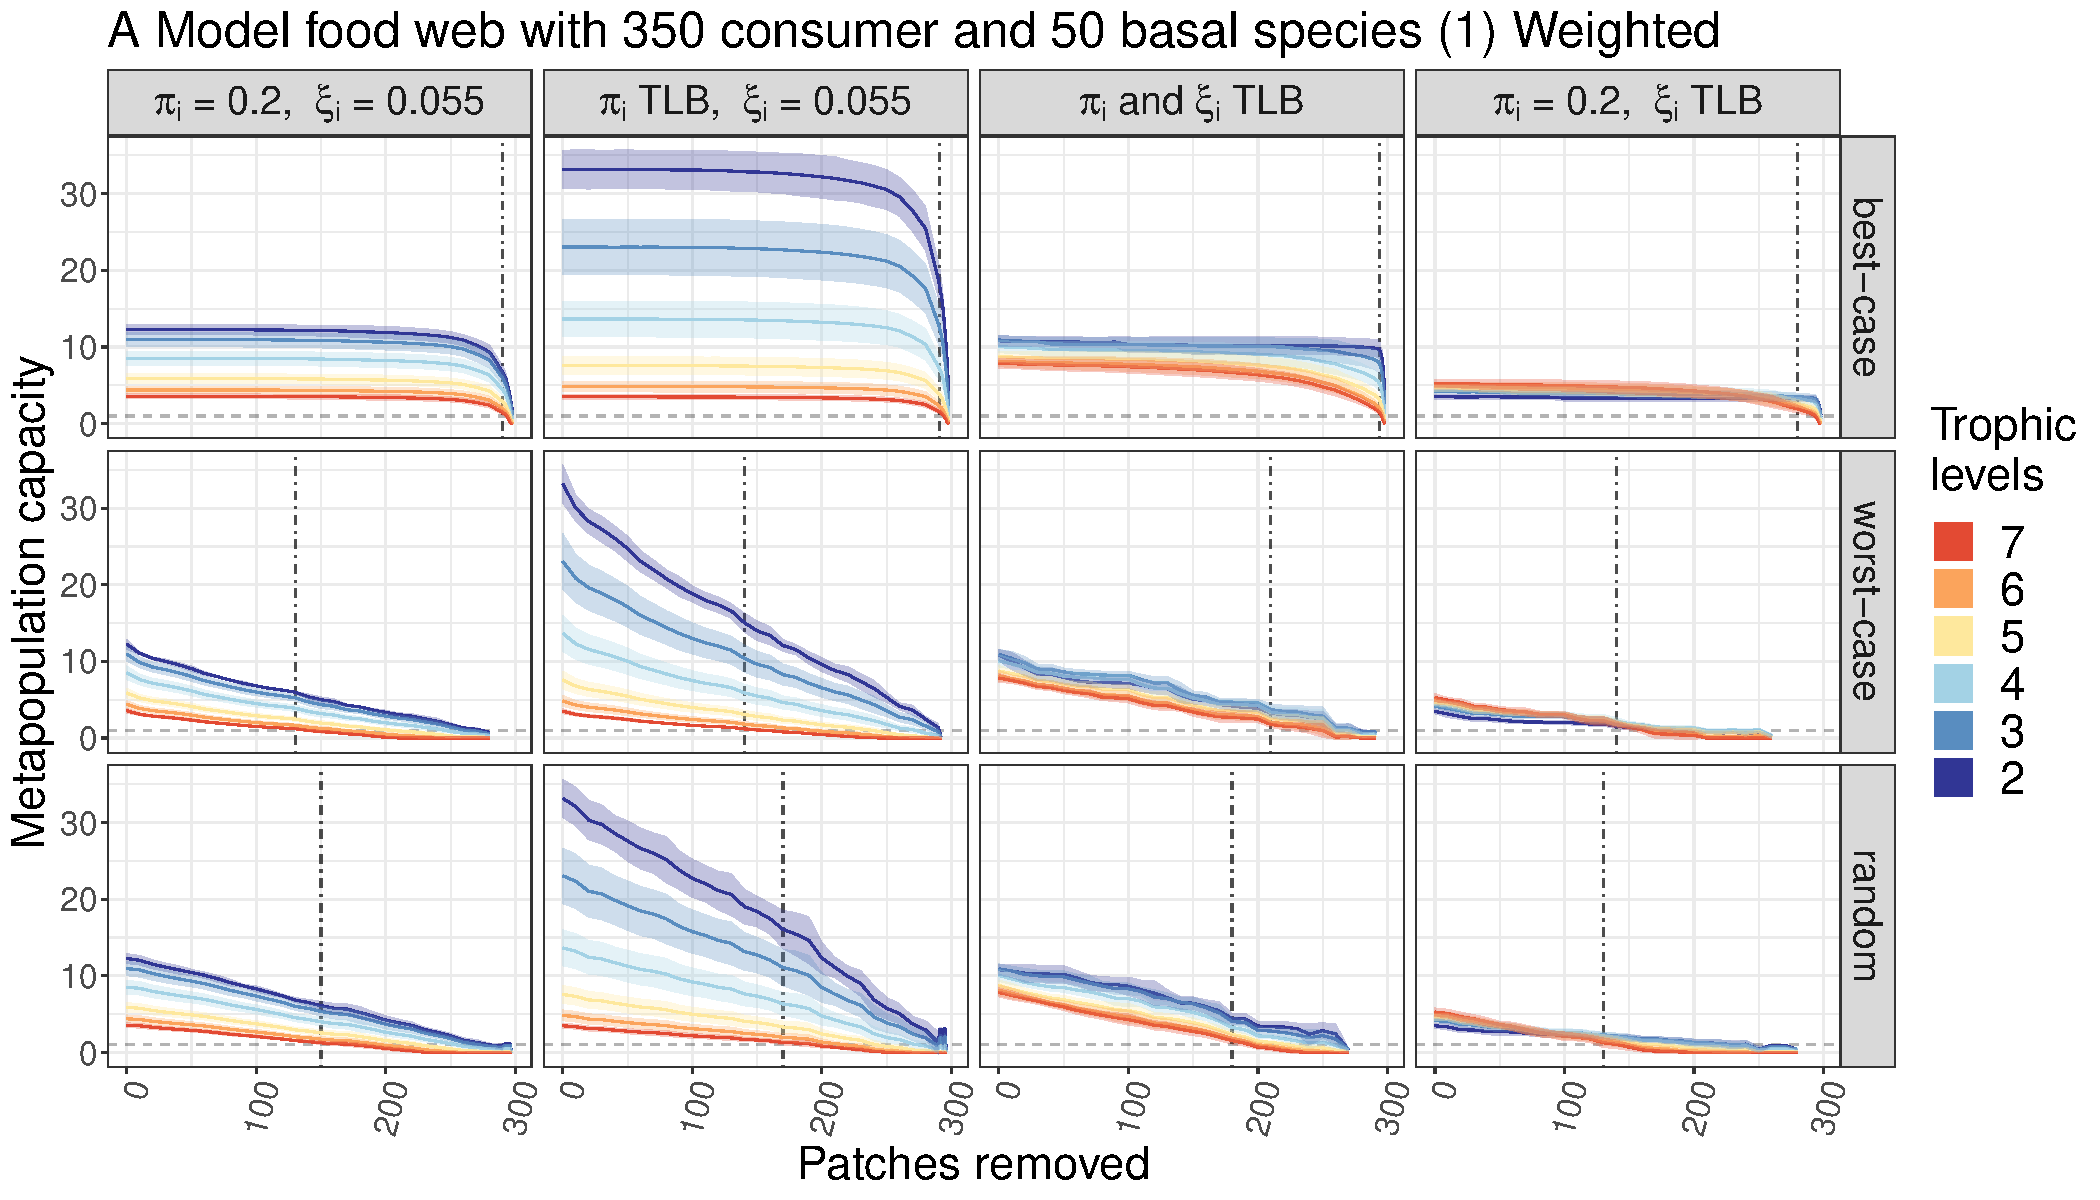
\includegraphics[width=0.8\textwidth,valign=t]{lambda_Model_food_web_with_350_consumer_and_50_basal_species_(1)_Weighted_basal_1_1.pdf}
  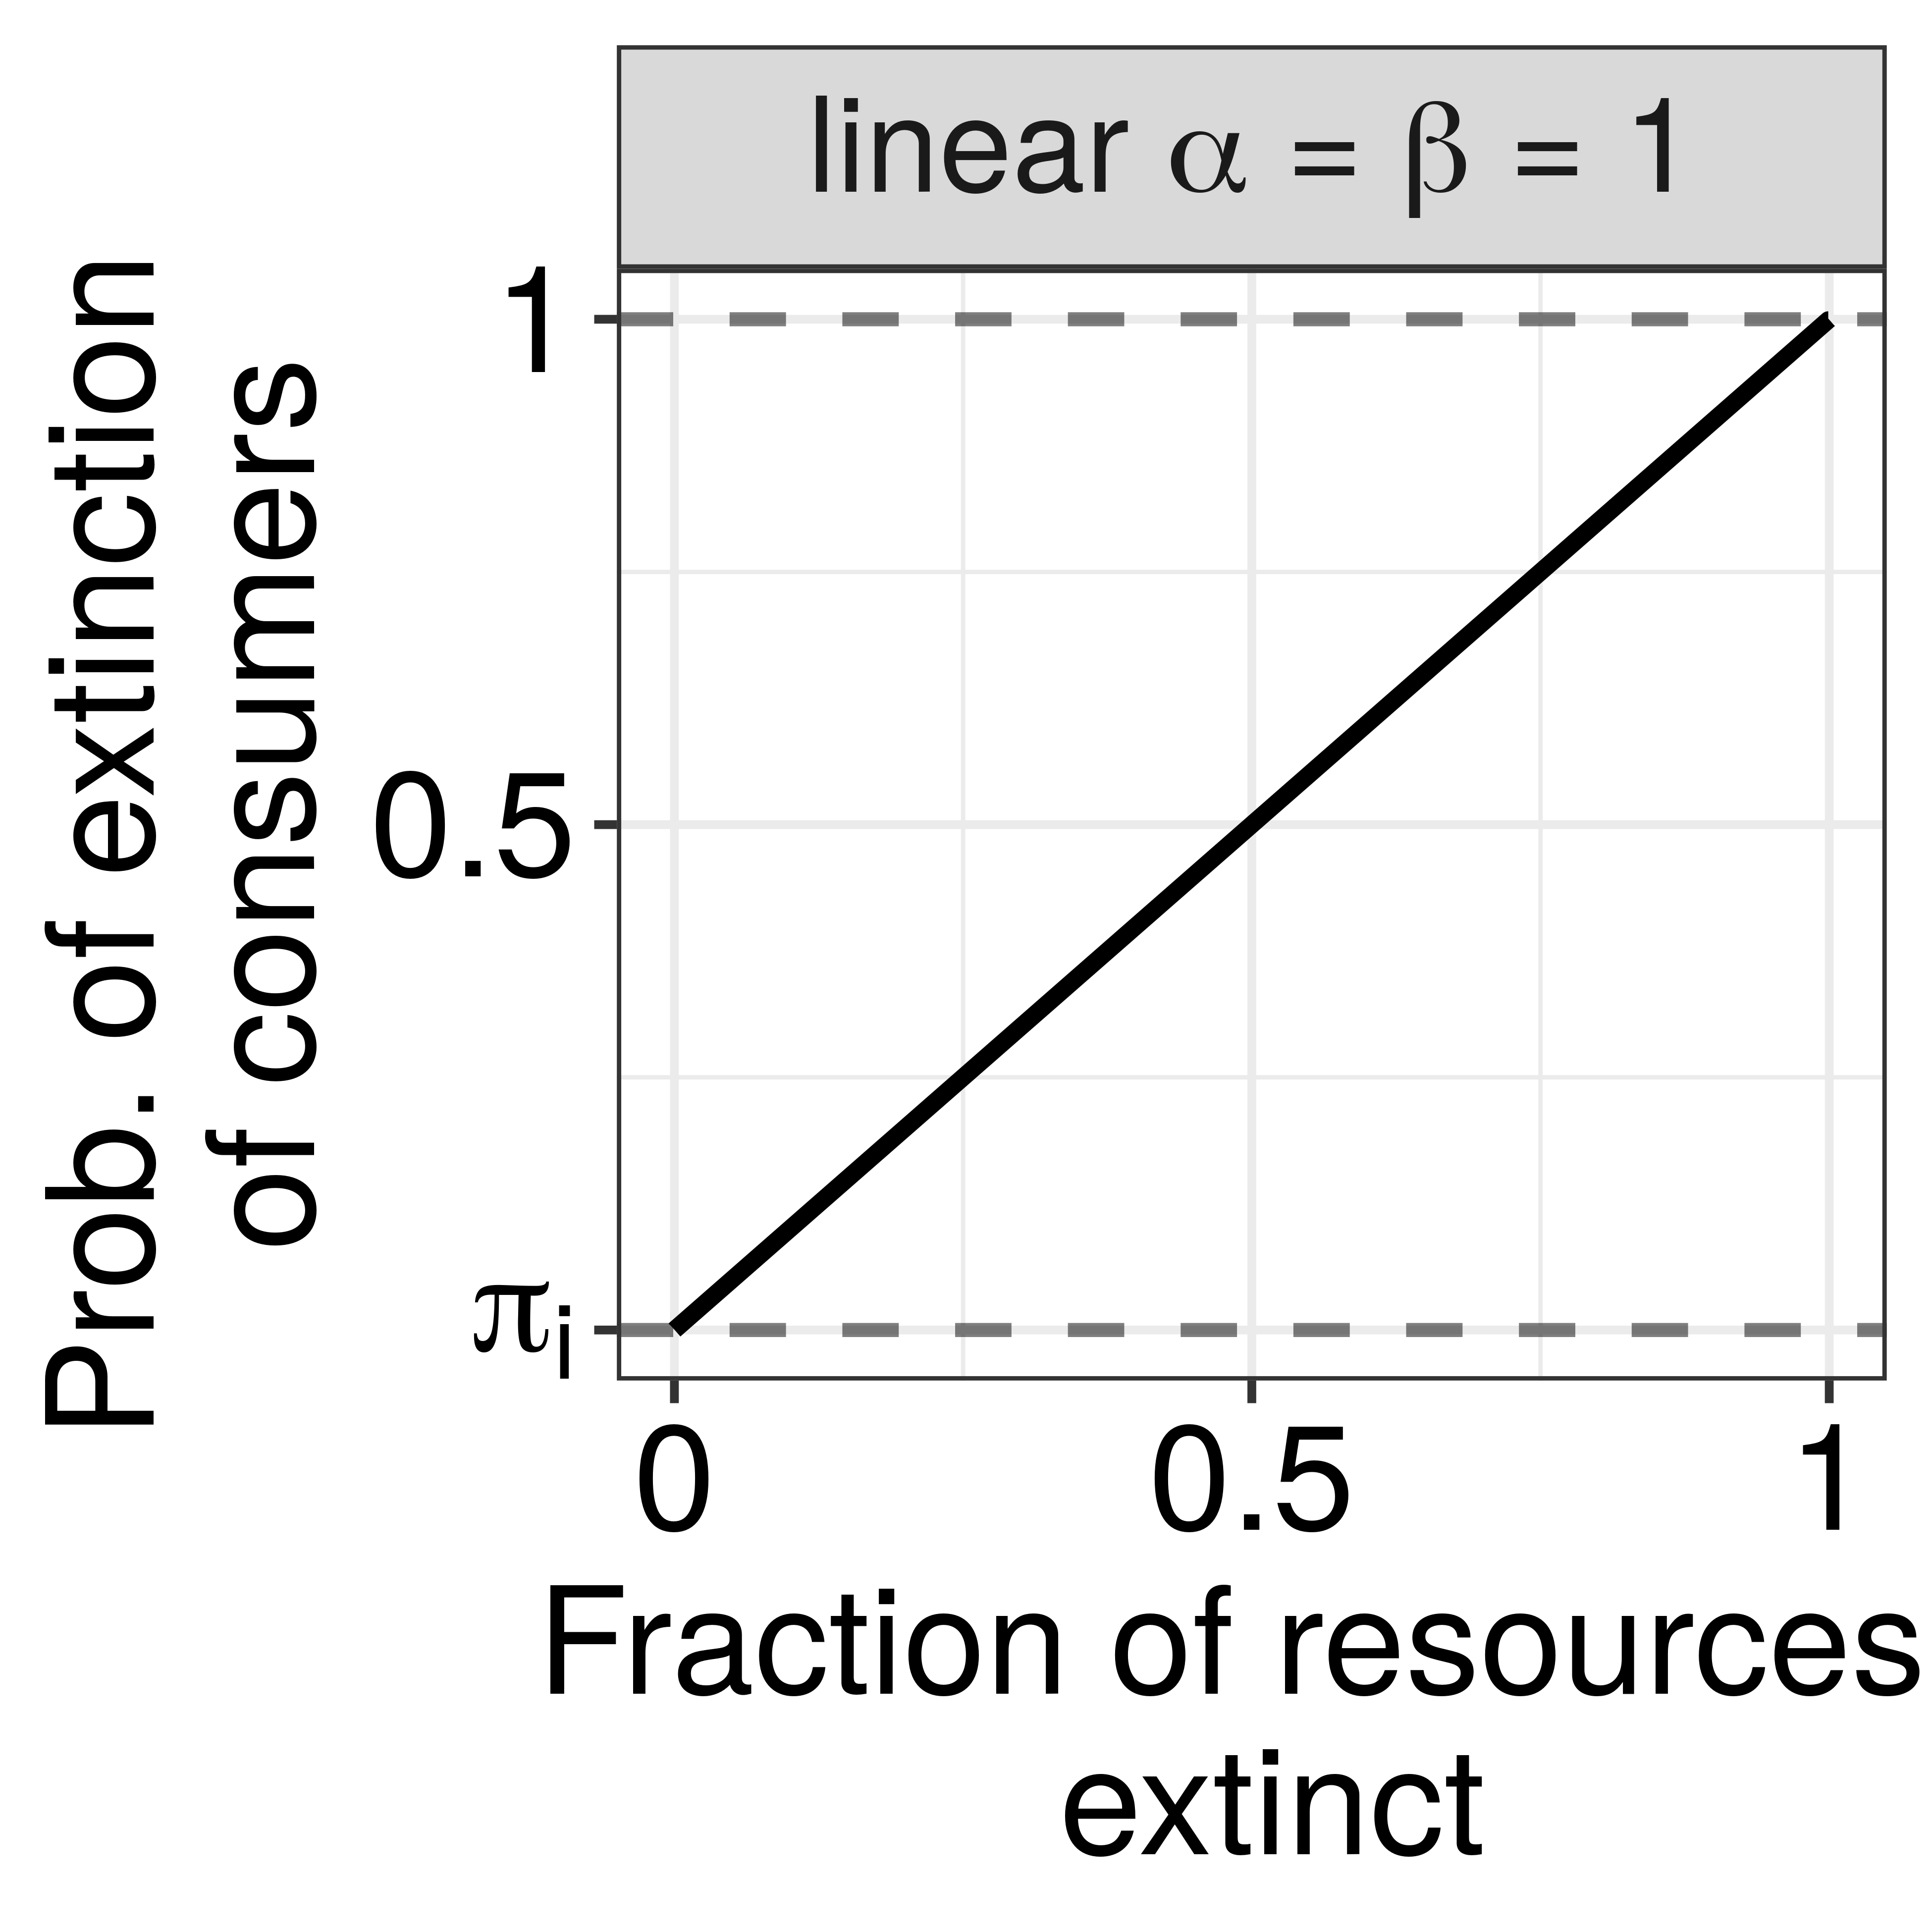
\includegraphics[width=0.19\textwidth,valign=t]{fform_1_1.png}
  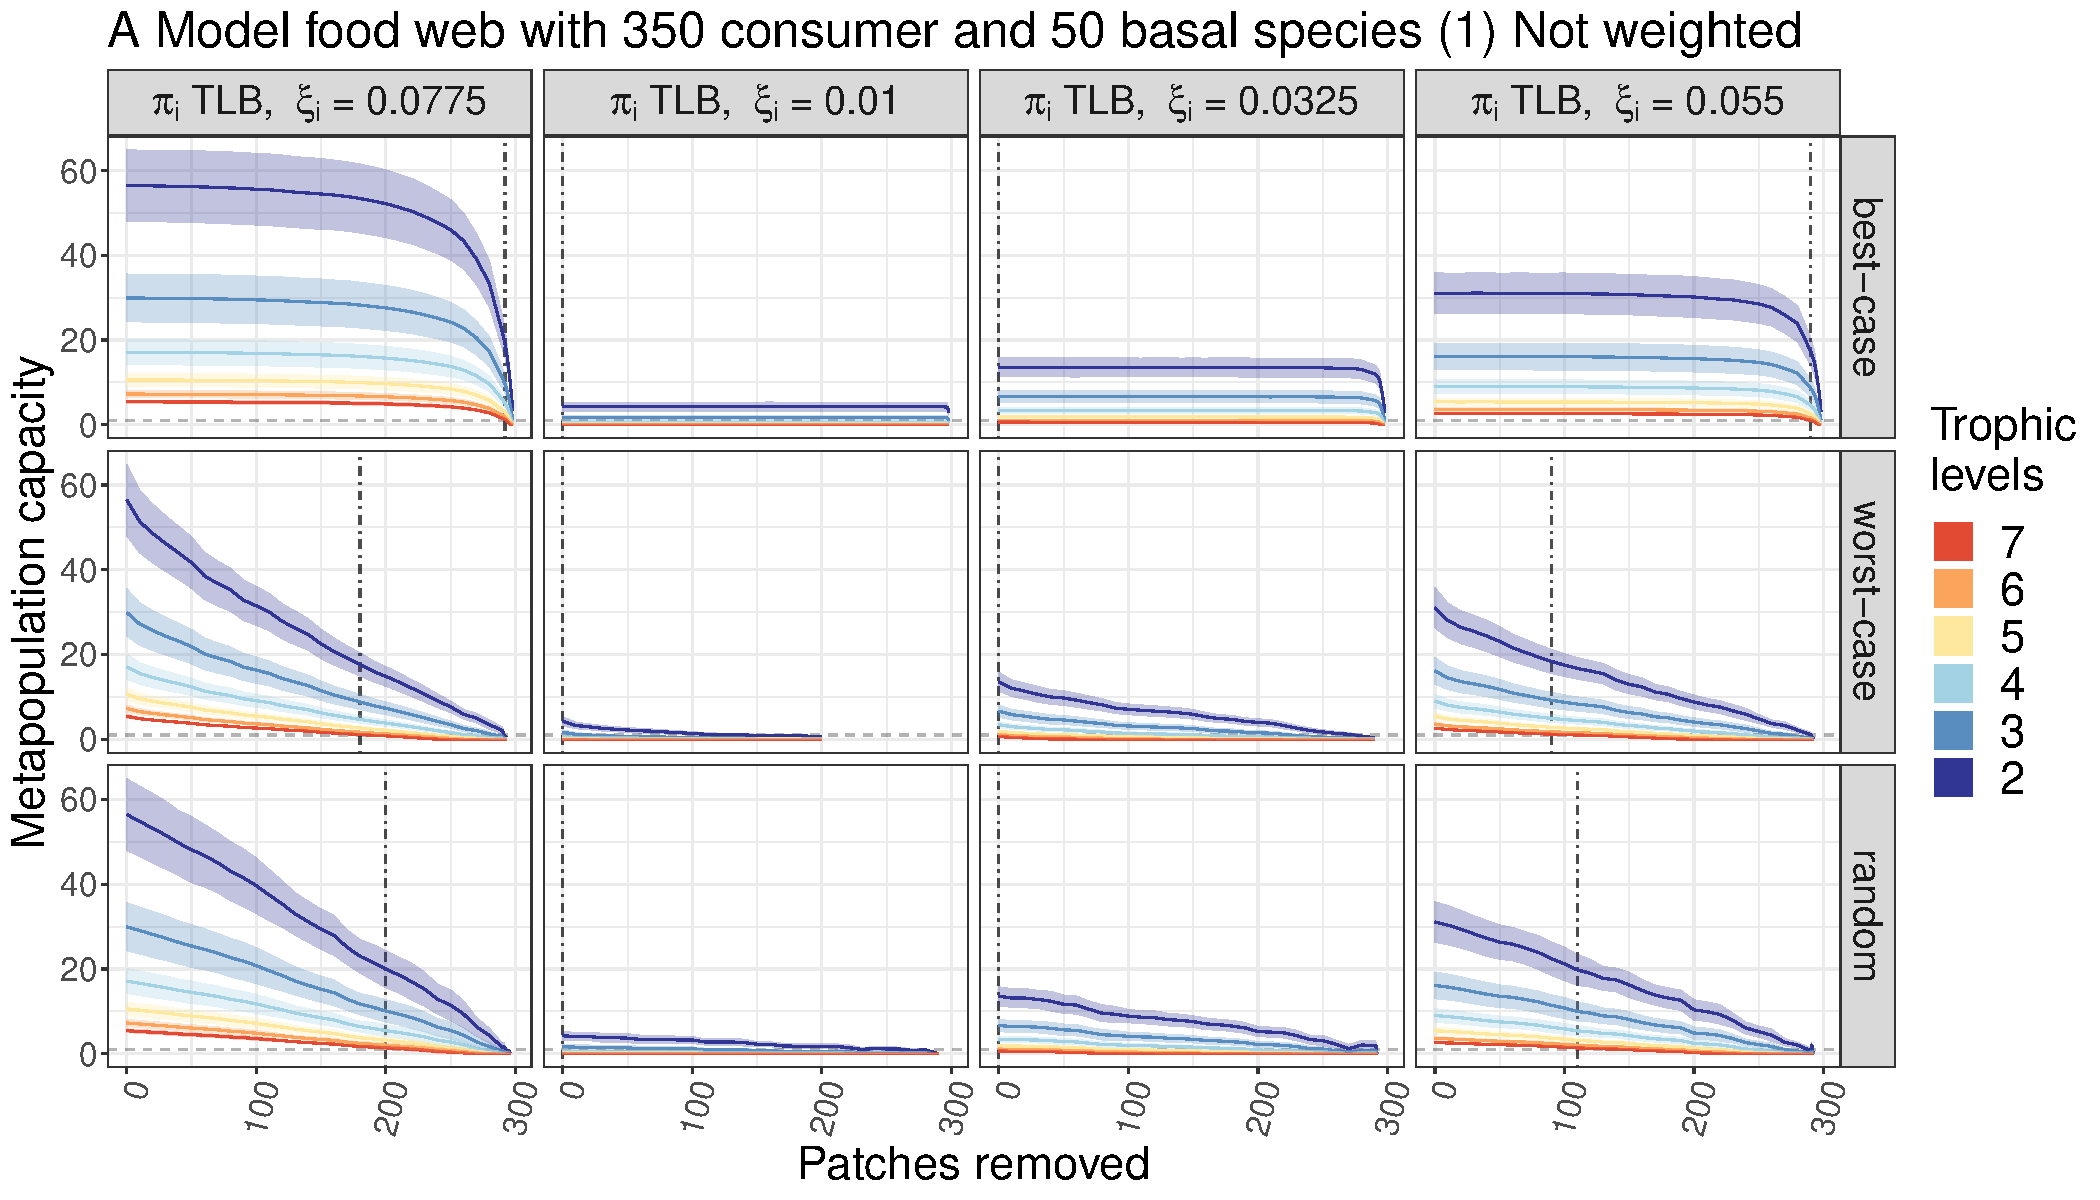
\includegraphics[width=0.8\textwidth,valign=t]{lambda_Model_food_web_with_350_consumer_and_50_basal_species_(1)_Not_weighted_basal_1_1.pdf}
  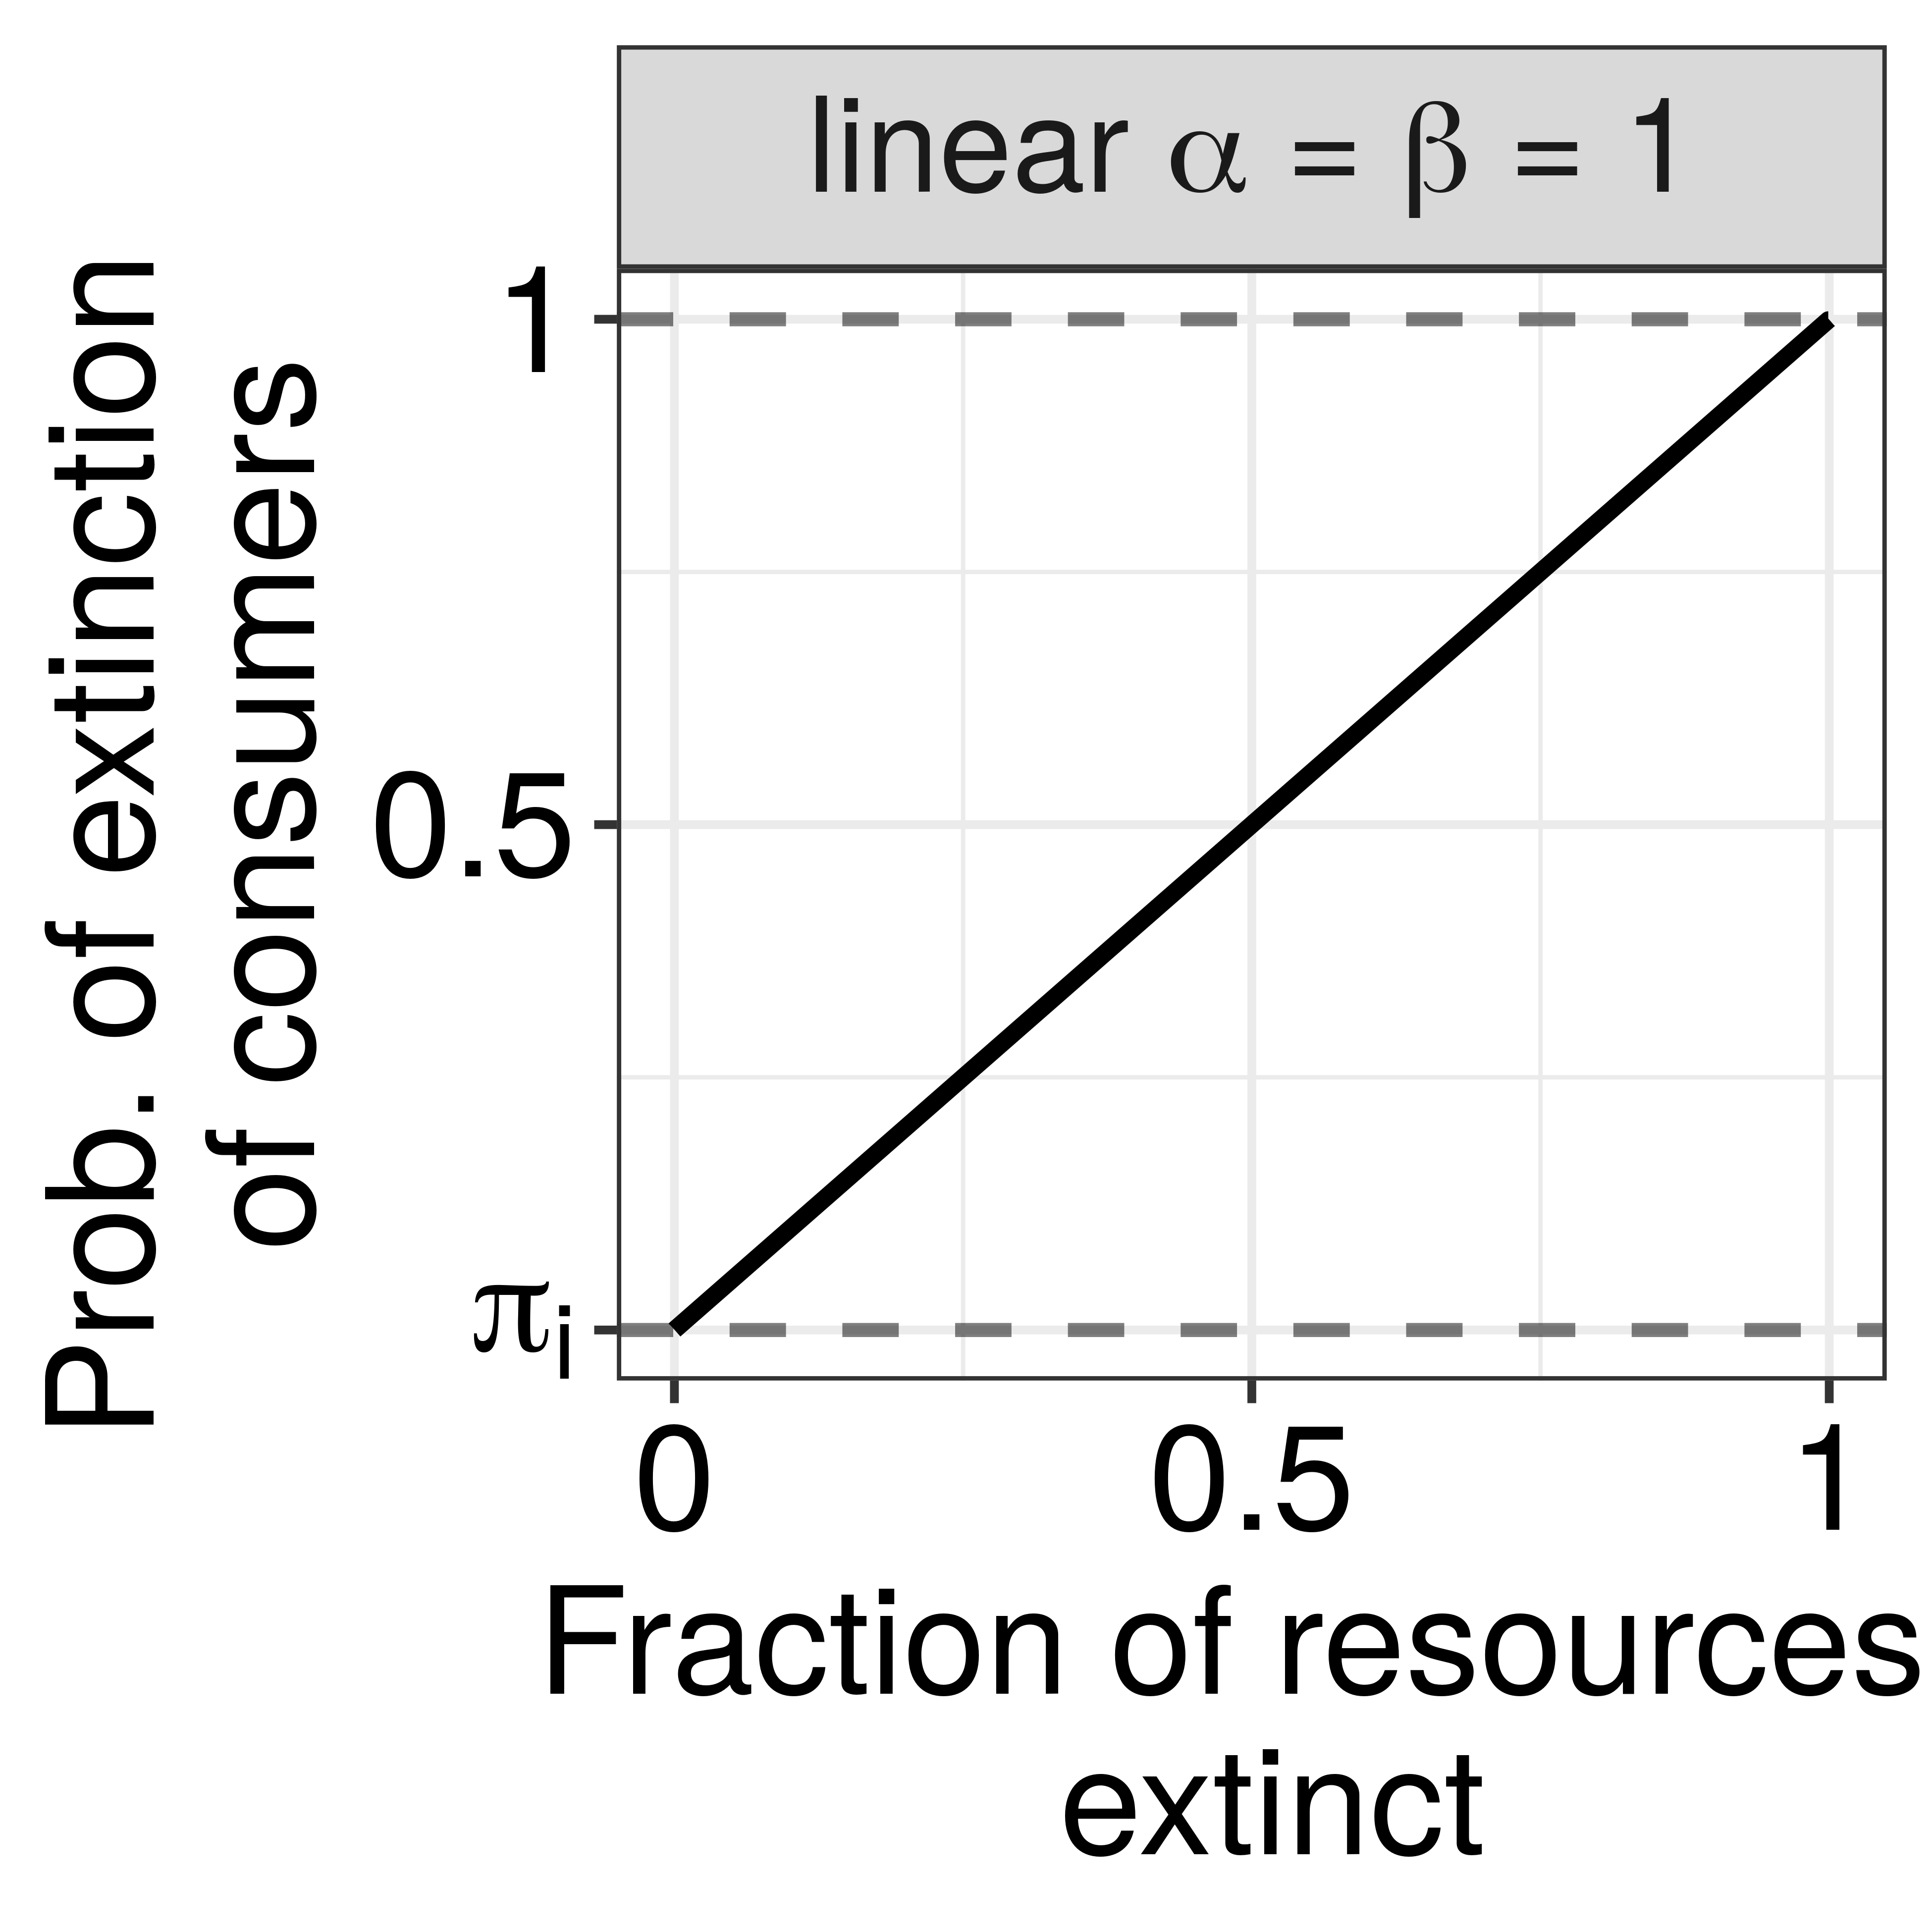
\includegraphics[width=0.19\textwidth,valign=t]{fform_1_1.png}
  \caption{Comparing the effect of habitat loss on species persistence in a weighted and not-weighted model food web with 350 consumer and 50 basal species. A-D are for different functional forms of a consumer's response to the loss of resources (top right insets). Species are grouped into trophic levels (color legends); lines show the mean and the bands around them the one standard deviation range of the metapopulation capacities of species in the corresponding trophic level. Rows indicate patch-removal scenario (best-case, worst-case, and random); columns the parameterization method: baseline extinction probabilities $\pi_i$ and dispersal distances $\xi_i$ can either take on one value across all species, or increase with trophic level (trophic level-based, TLB). Horizontal dashed lines highlight a metapopulation capacity of $1$, the threshold for long-term species persistence. Vertical dashed lines show when the metapopulation capacity of the top species in the food web drops below this threshold.}
  \label{fig:patchloss_web1_11}
\end{figure}

\begin{figure}\ContinuedFloat
  \includegraphics[width=0.8\textwidth,valign=t]{lambda_Model_food_web_with_350_consumer_and_50_basal_species_(1)_Weighted_basal_5_1.pdf}
  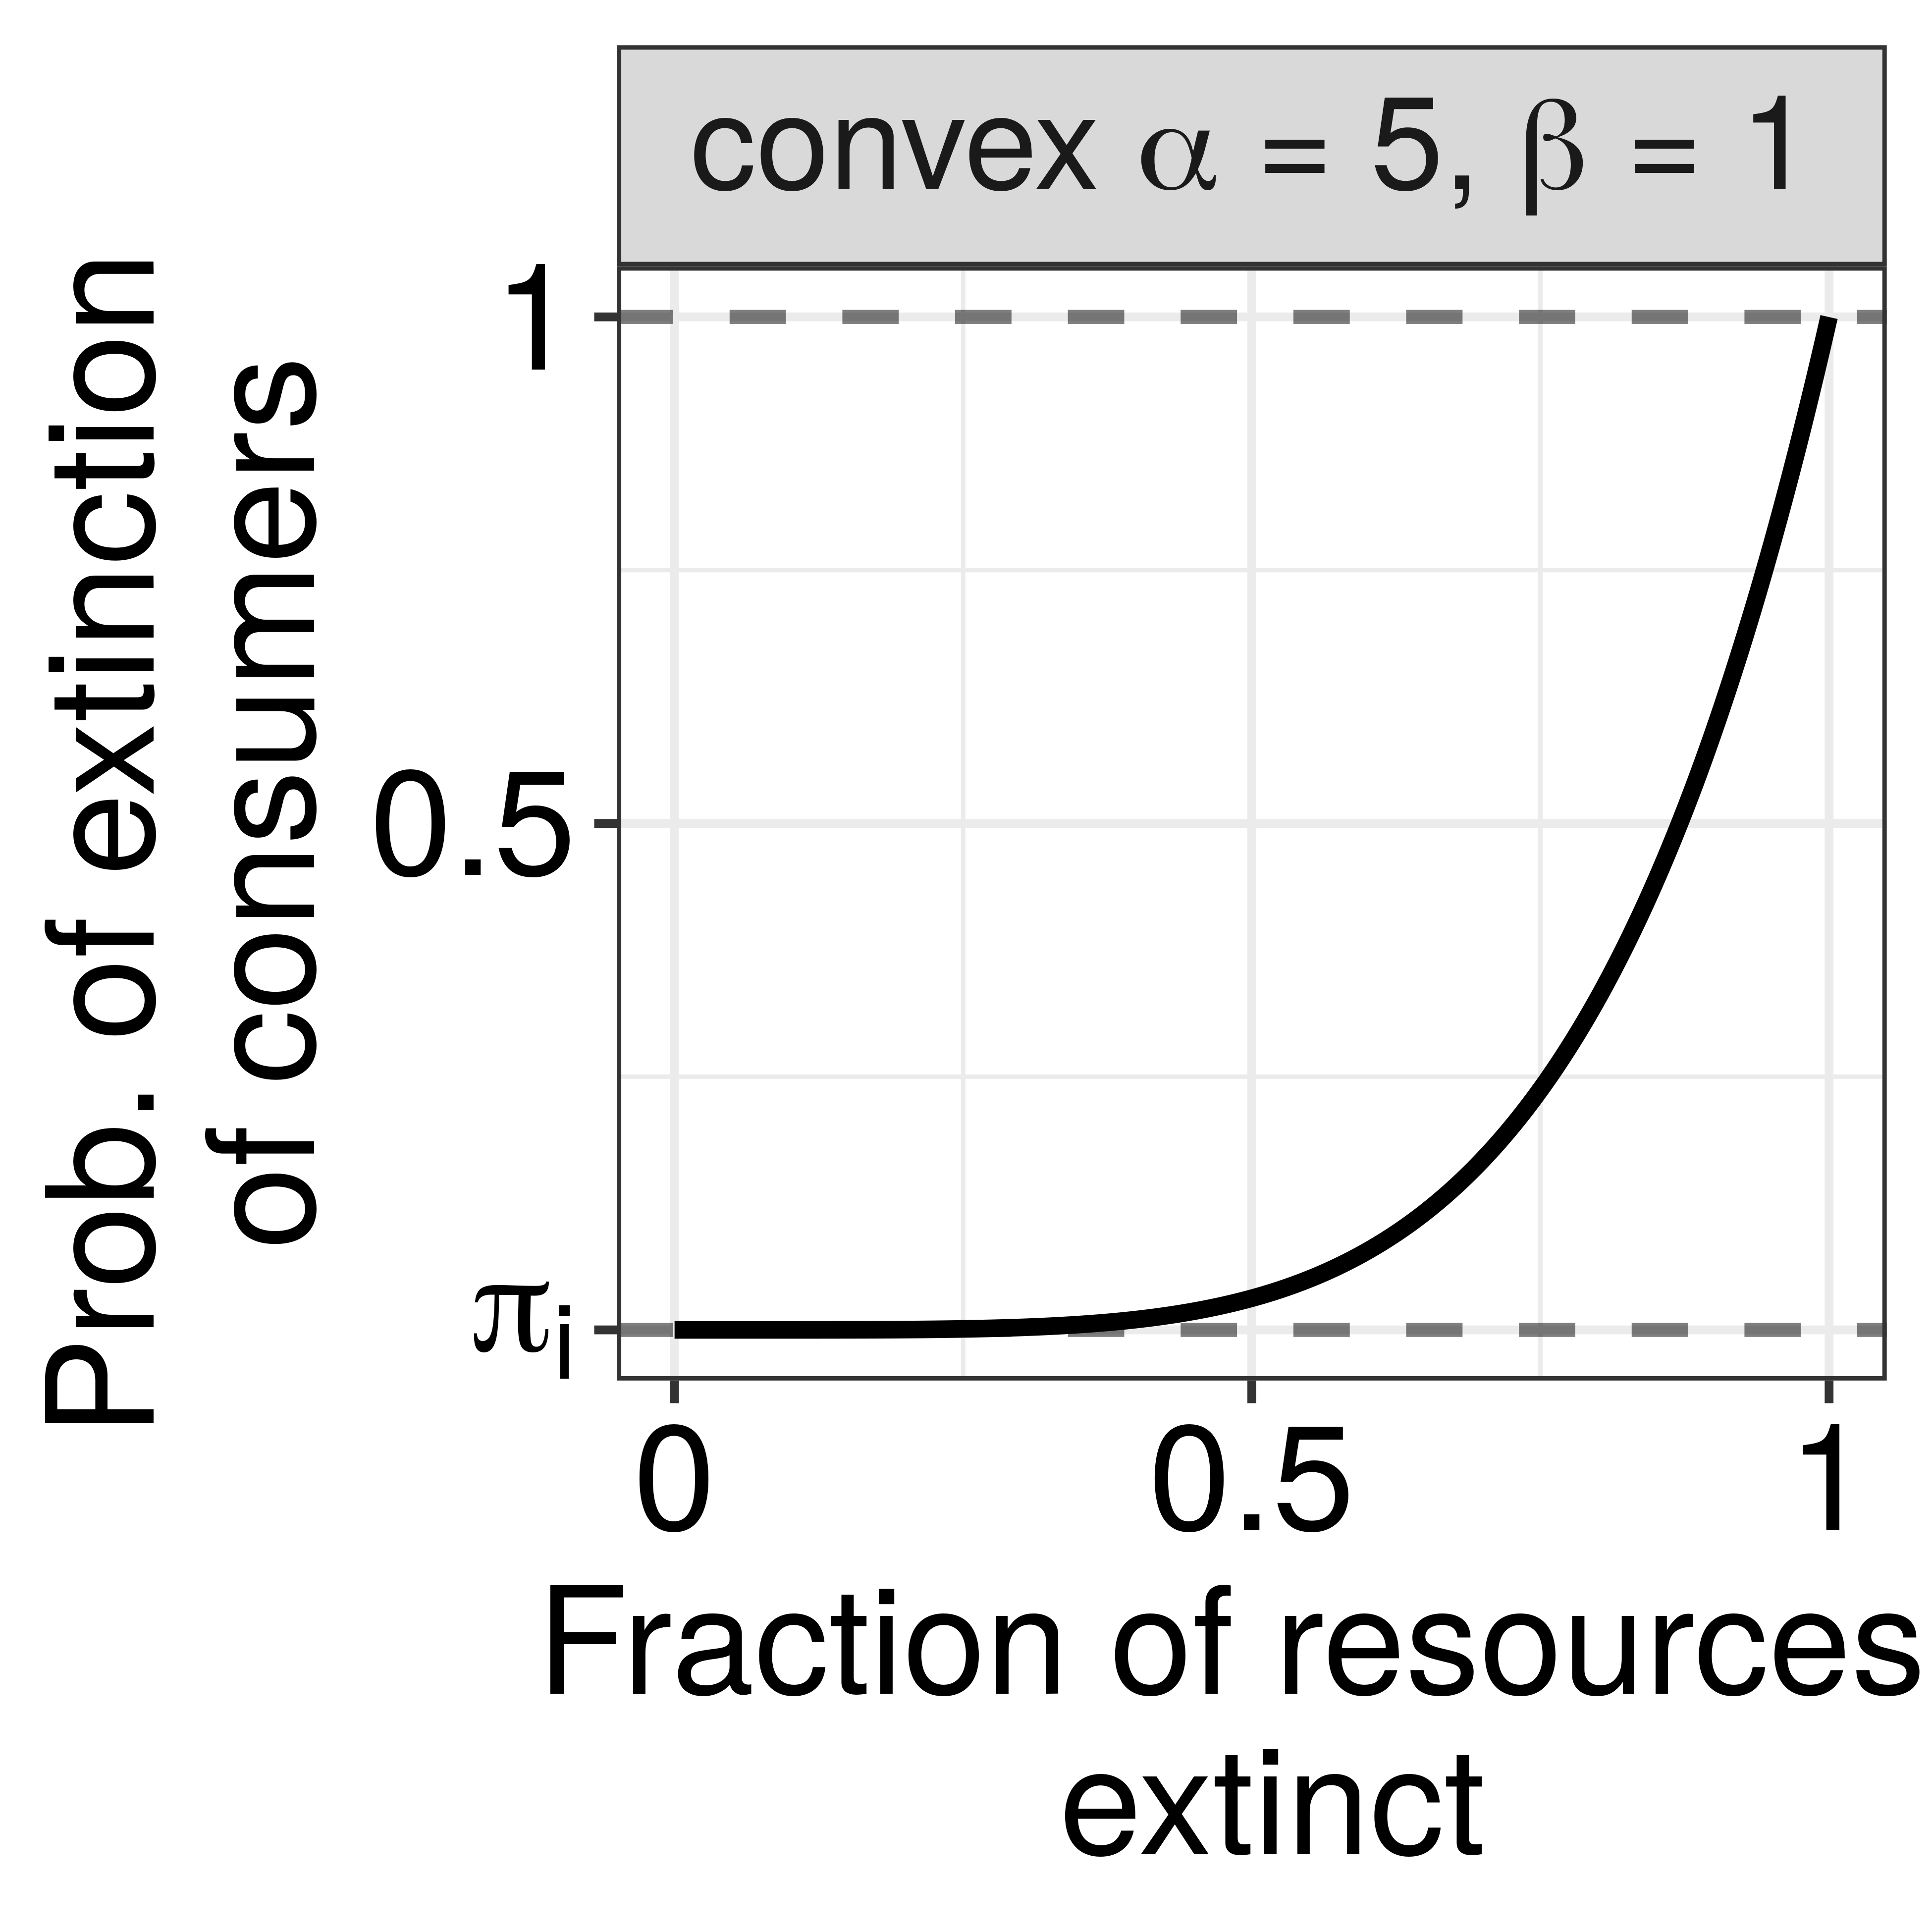
\includegraphics[width=0.19\textwidth,valign=t]{fform_5_1.png}
  \includegraphics[width=0.8\textwidth,valign=t]{lambda_Model_food_web_with_350_consumer_and_50_basal_species_(1)_Not_weighted_basal_5_1.pdf}
  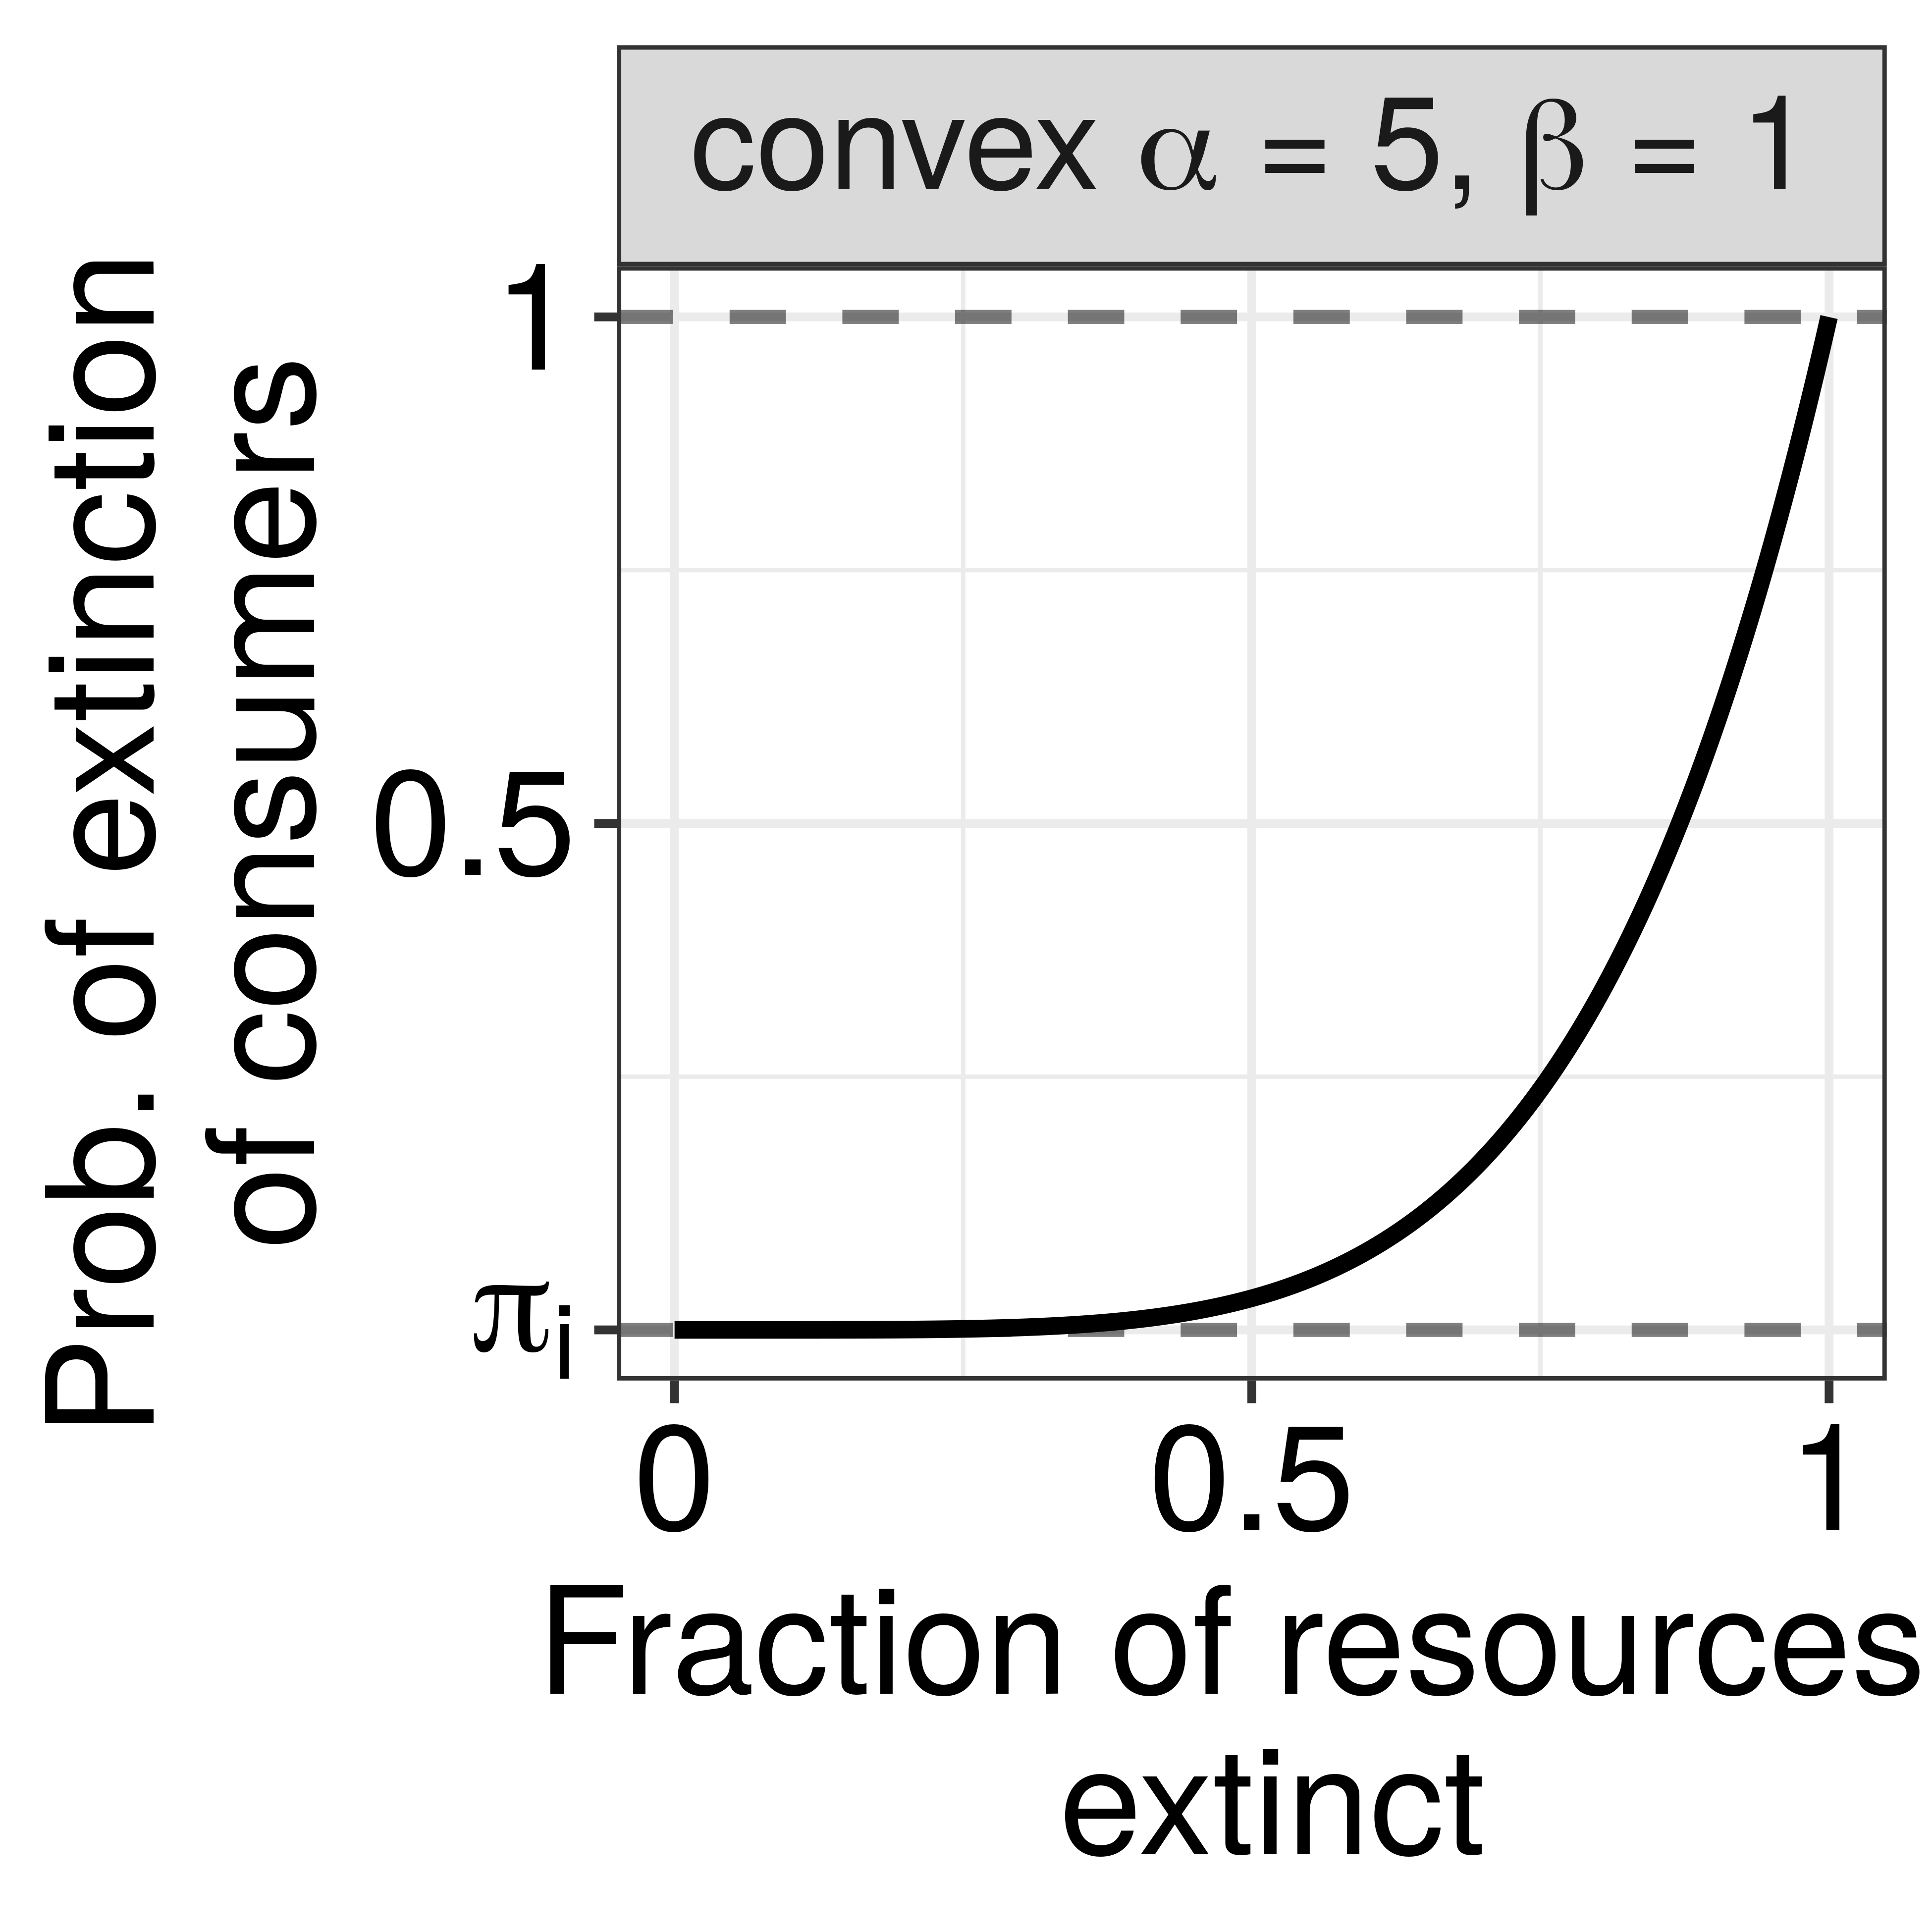
\includegraphics[width=0.19\textwidth,valign=t]{fform_5_1.png}
  \caption{Figure continued.}
  \label{fig:patchloss_web1_51}
\end{figure}

\begin{figure}\ContinuedFloat
  \includegraphics[width=0.8\textwidth,valign=t]{lambda_Model_food_web_with_350_consumer_and_50_basal_species_(1)_Weighted_basal_1_5.pdf}
  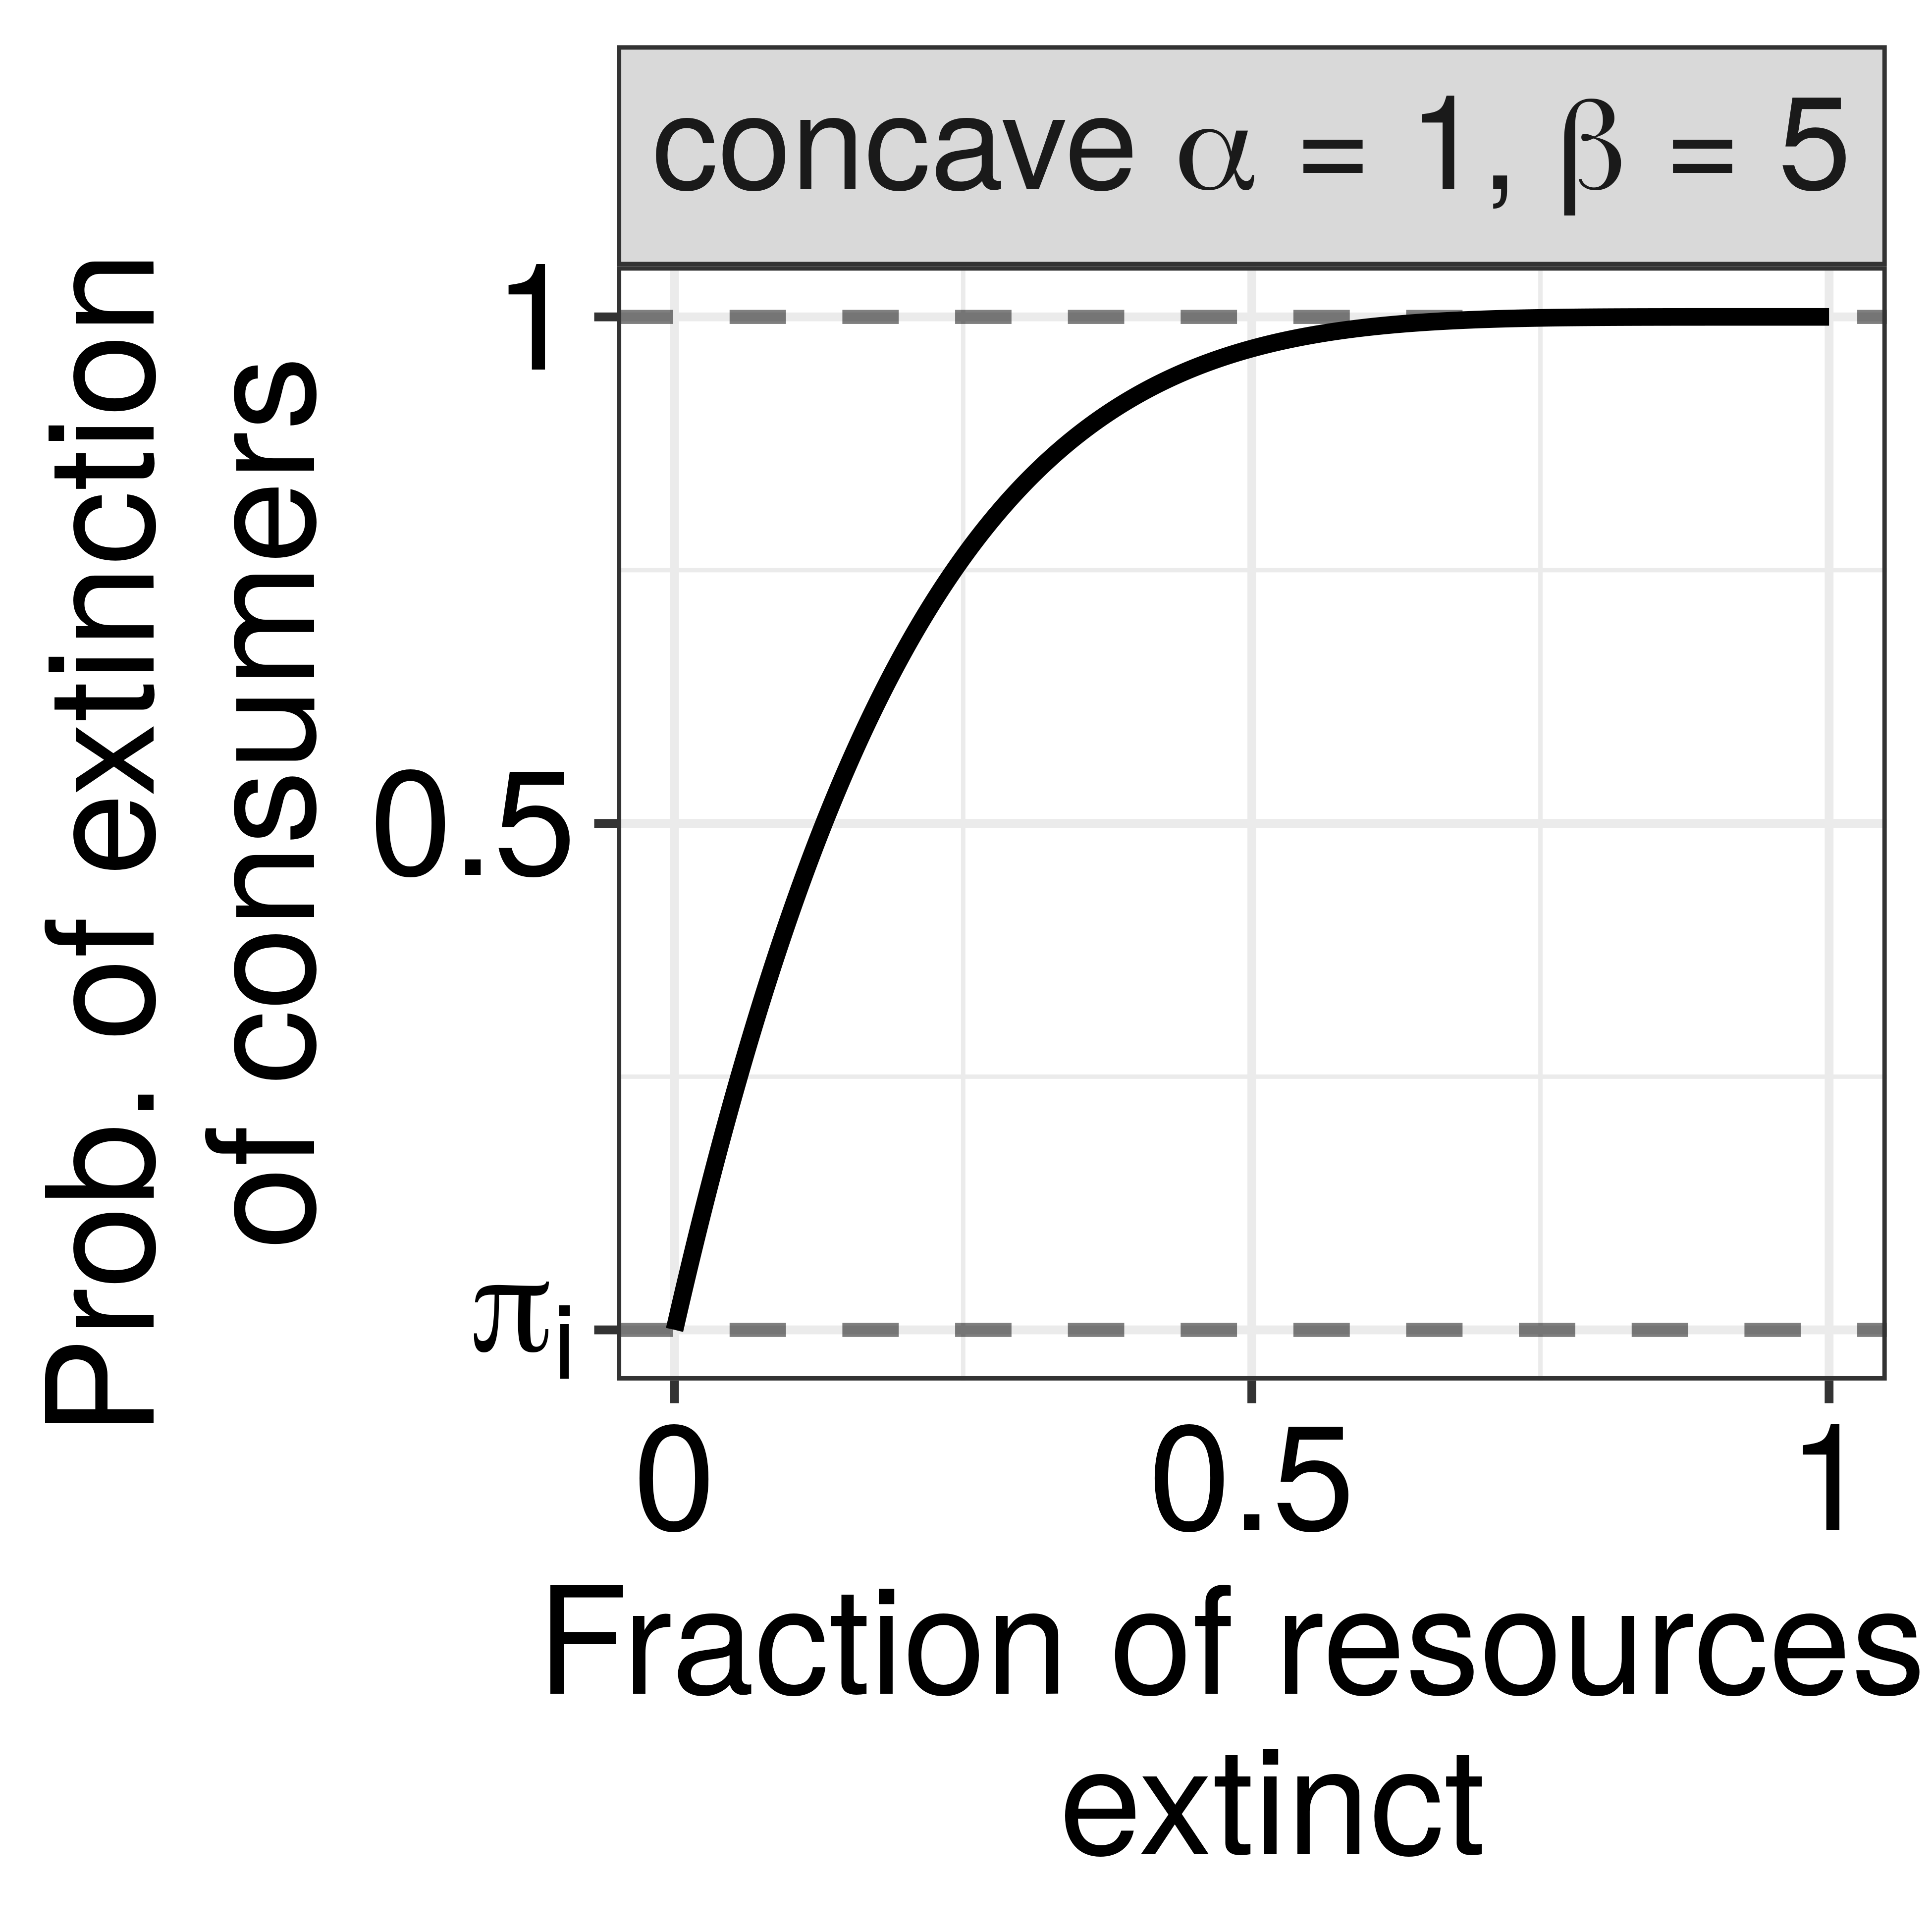
\includegraphics[width=0.19\textwidth,valign=t]{fform_1_5.png}
  \includegraphics[width=0.8\textwidth,valign=t]{lambda_Model_food_web_with_350_consumer_and_50_basal_species_(1)_Not_weighted_basal_1_5.pdf}
  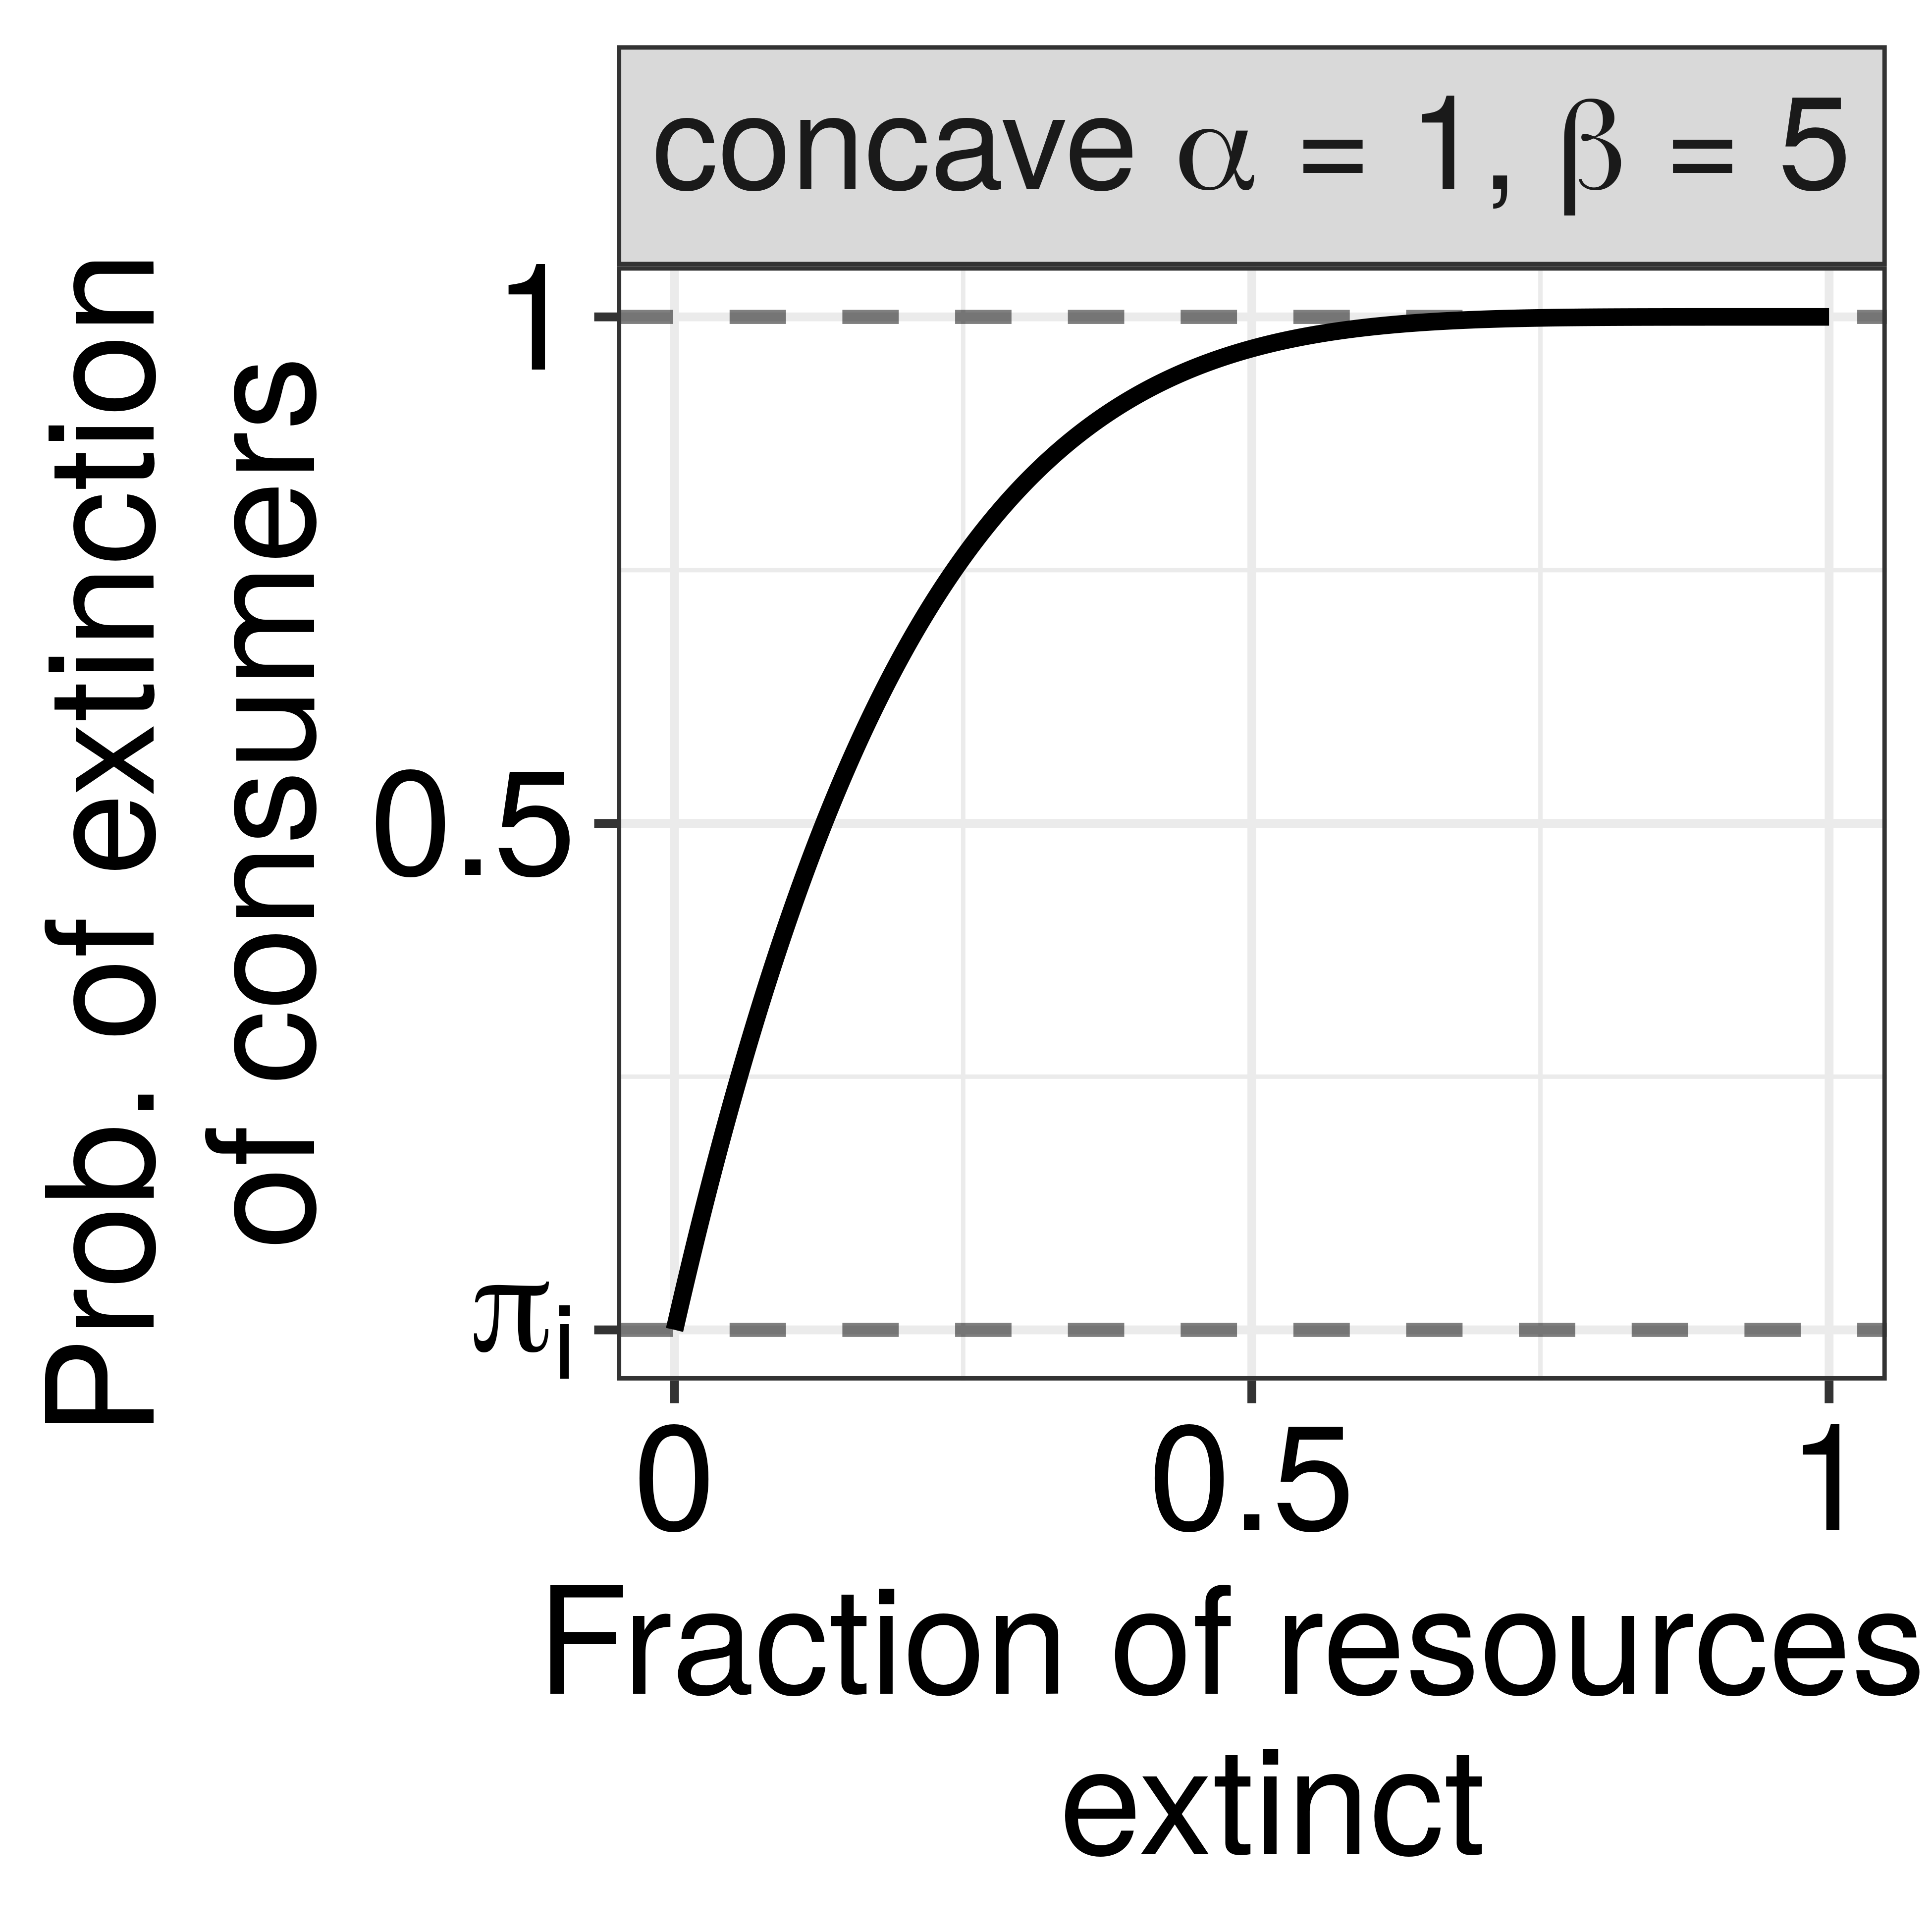
\includegraphics[width=0.19\textwidth,valign=t]{fform_1_5.png}
  \caption{Figure continued.}
  \label{fig:patchloss_web1_15}
\end{figure}

\begin{figure}\ContinuedFloat
  \includegraphics[width=0.8\textwidth,valign=t]{lambda_Model_food_web_with_350_consumer_and_50_basal_species_(1)_Weighted_basal_5_5.pdf}
  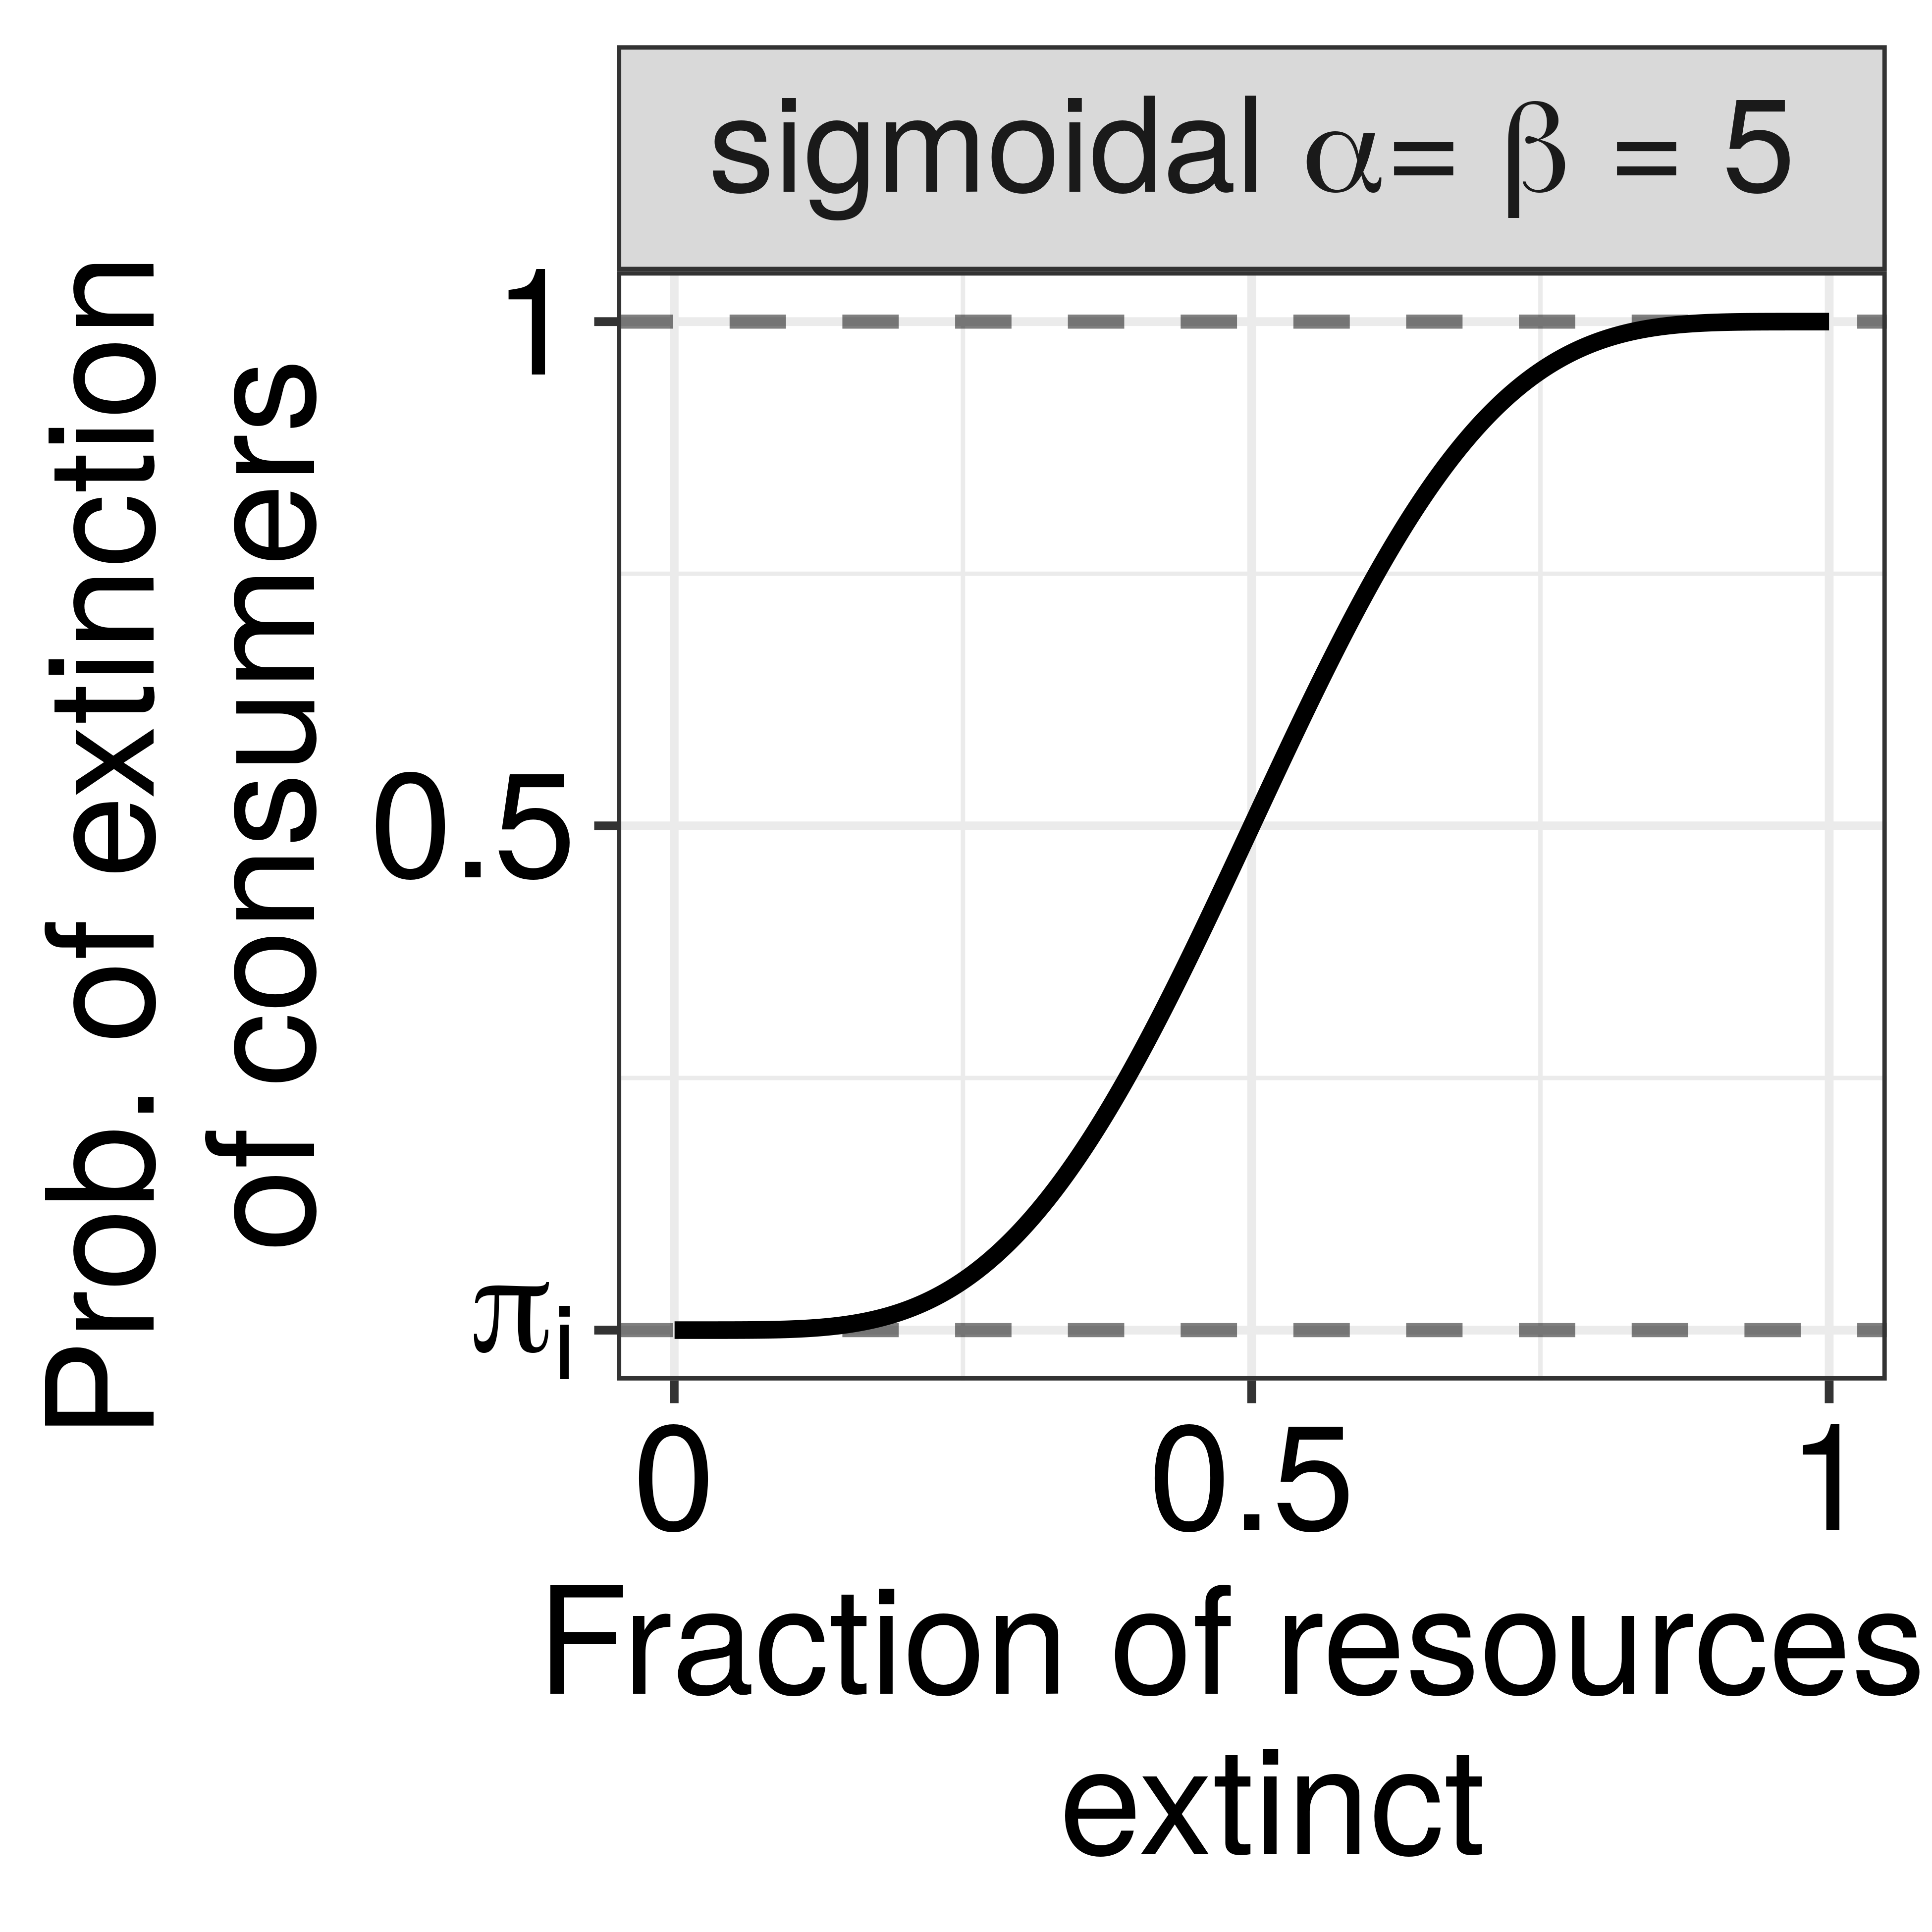
\includegraphics[width=0.19\textwidth,valign=t]{fform_5_5.png}
  \includegraphics[width=0.8\textwidth,valign=t]{lambda_Model_food_web_with_350_consumer_and_50_basal_species_(1)_Not_weighted_basal_5_5.pdf}
  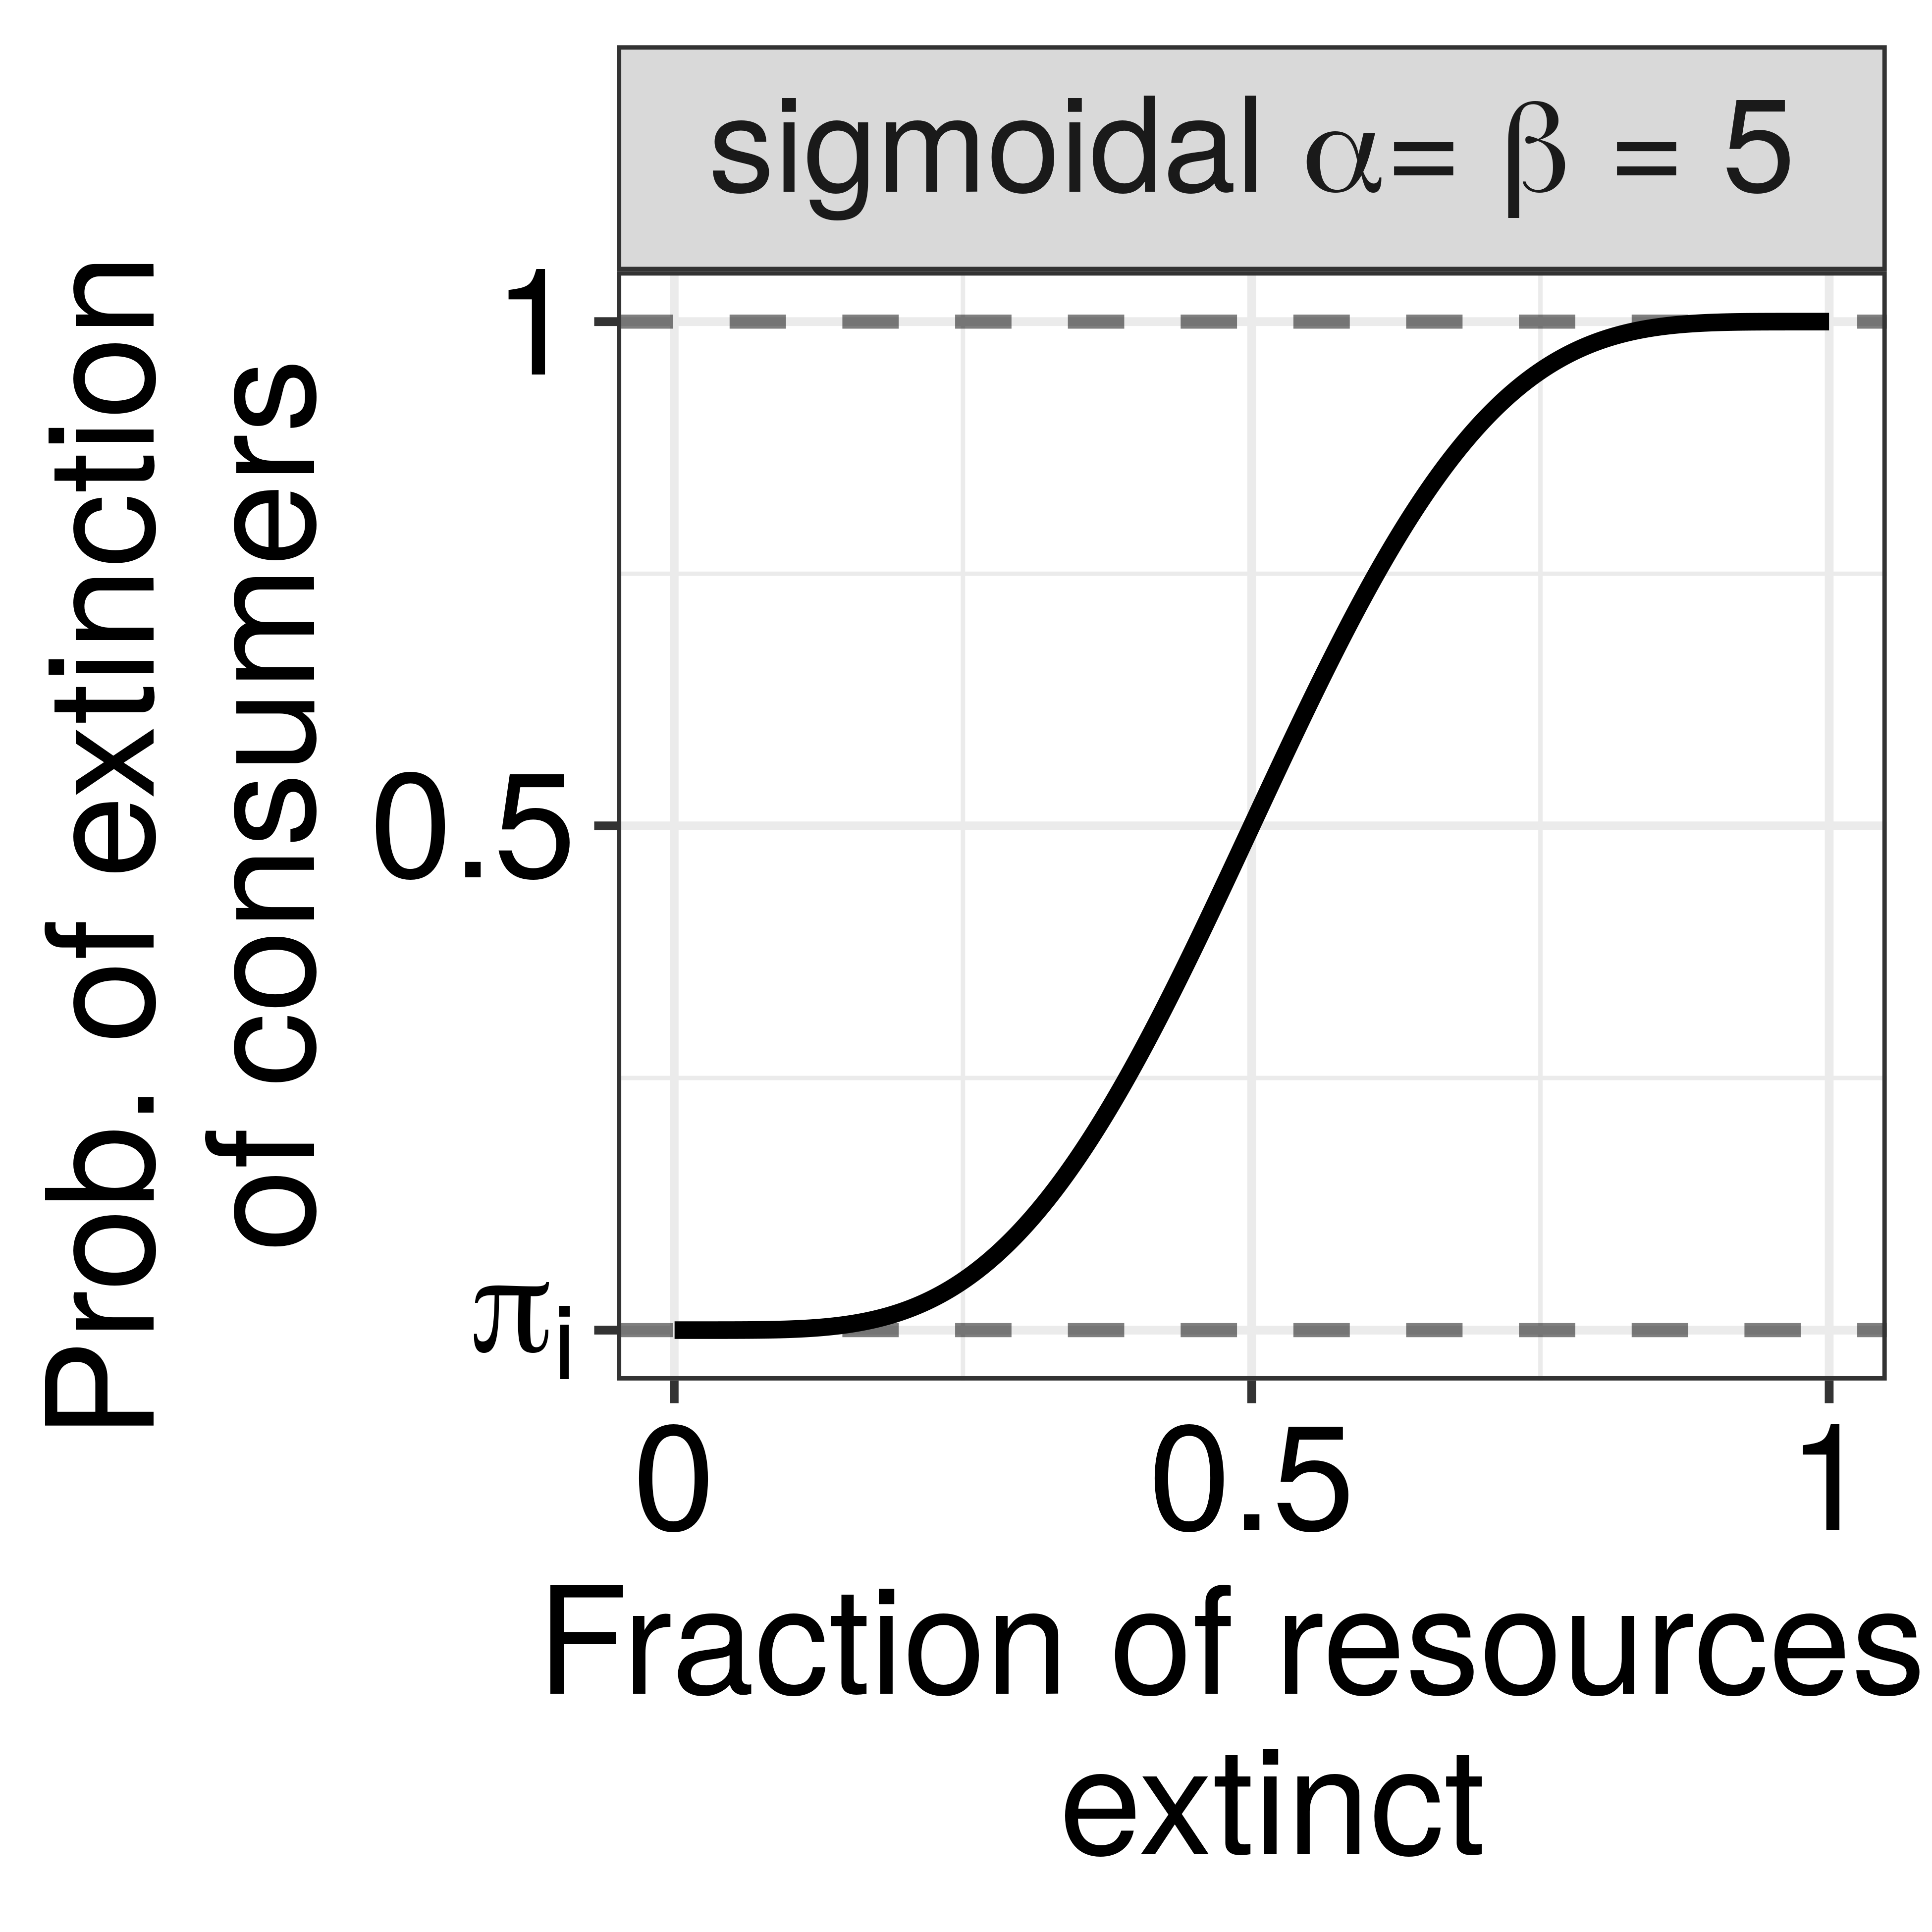
\includegraphics[width=0.19\textwidth,valign=t]{fform_5_5.png}
  \caption{Figure continued.}
  \label{fig:patchloss_web1_55}
\end{figure}

\begin{figure}
  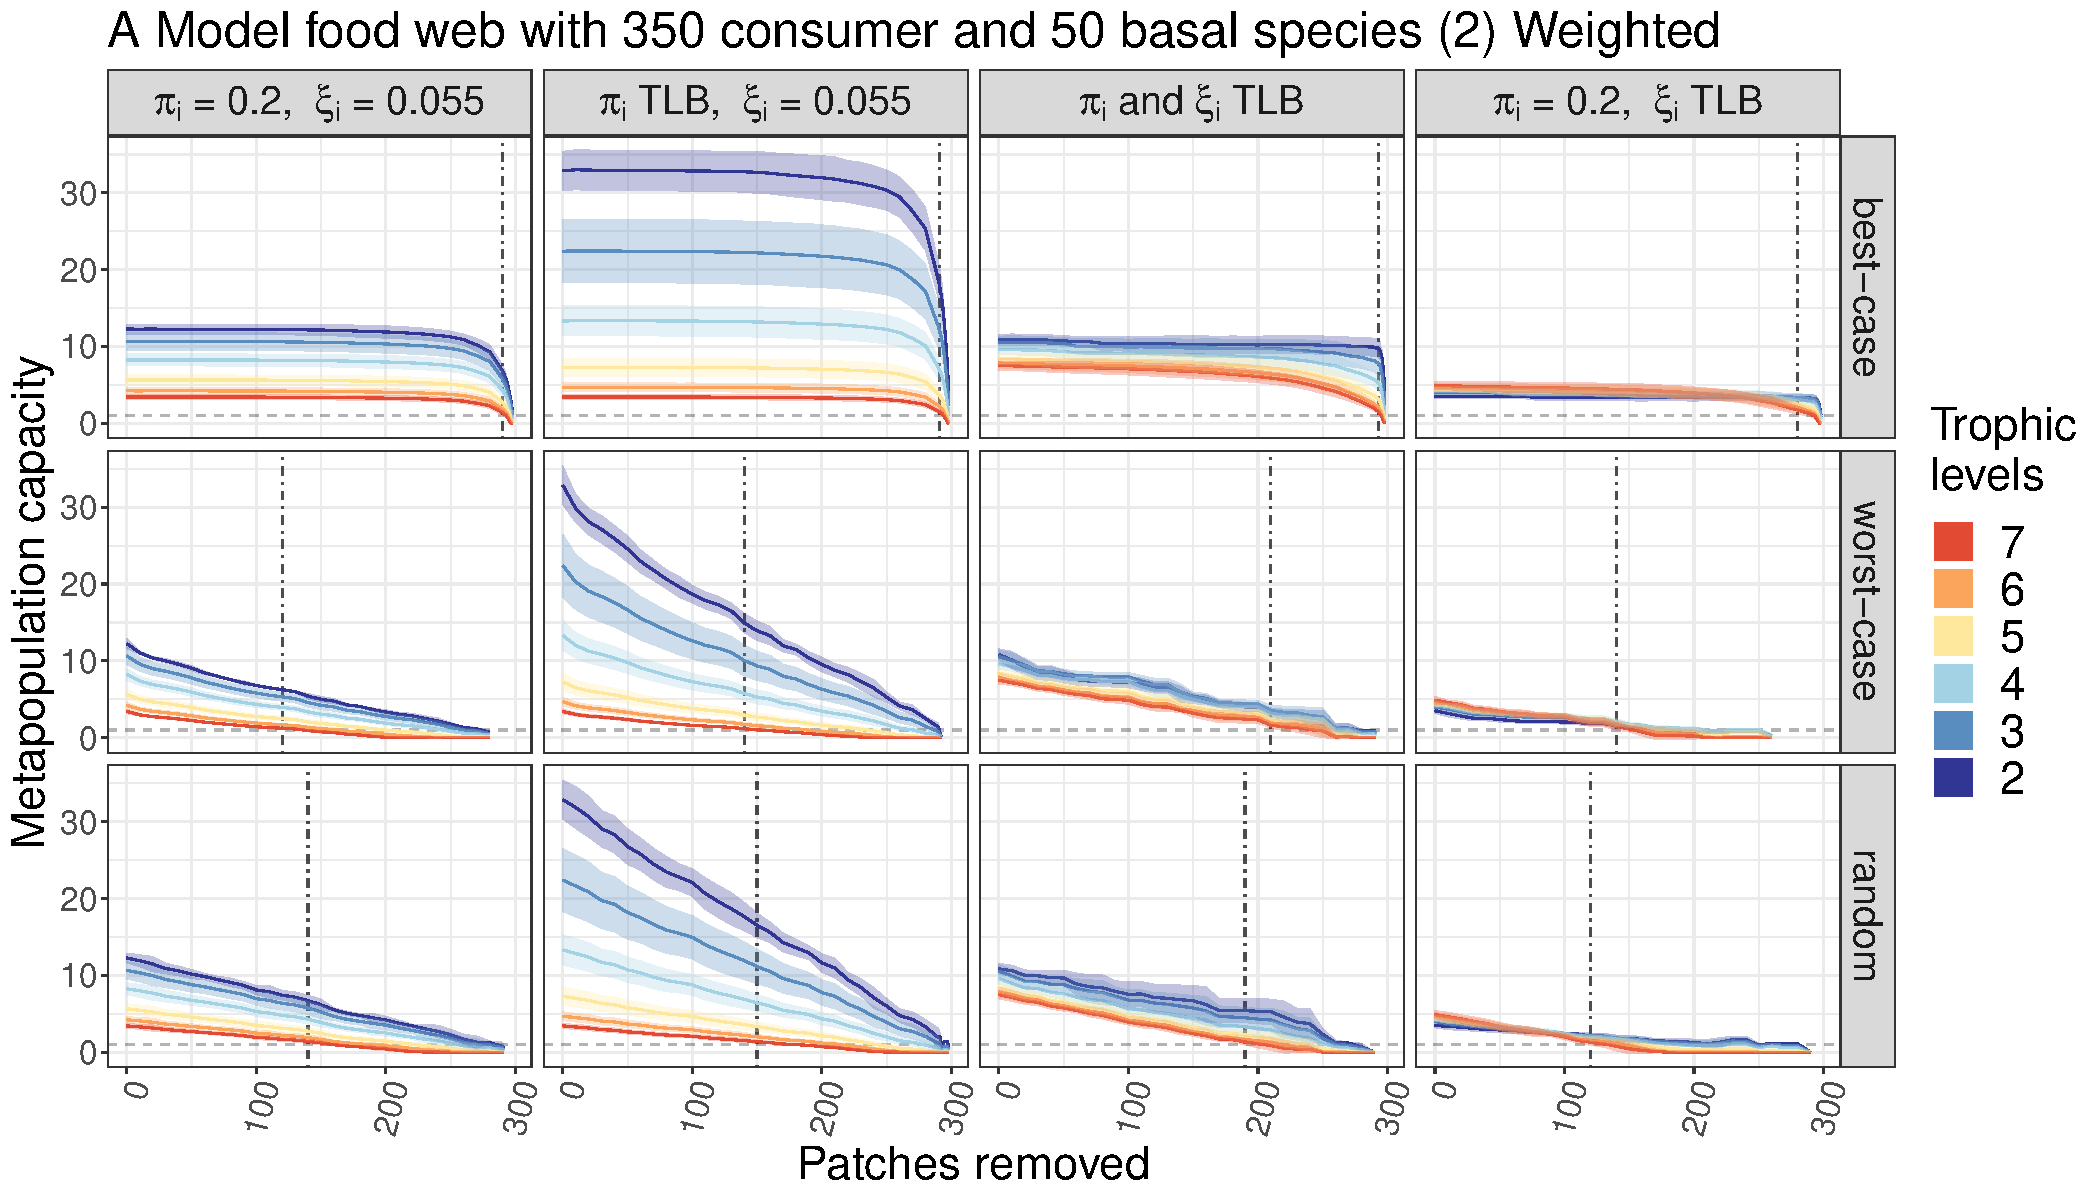
\includegraphics[width=0.8\textwidth,valign=t]{lambda_Model_food_web_with_350_consumer_and_50_basal_species_(2)_Weighted_basal_1_1.pdf}
  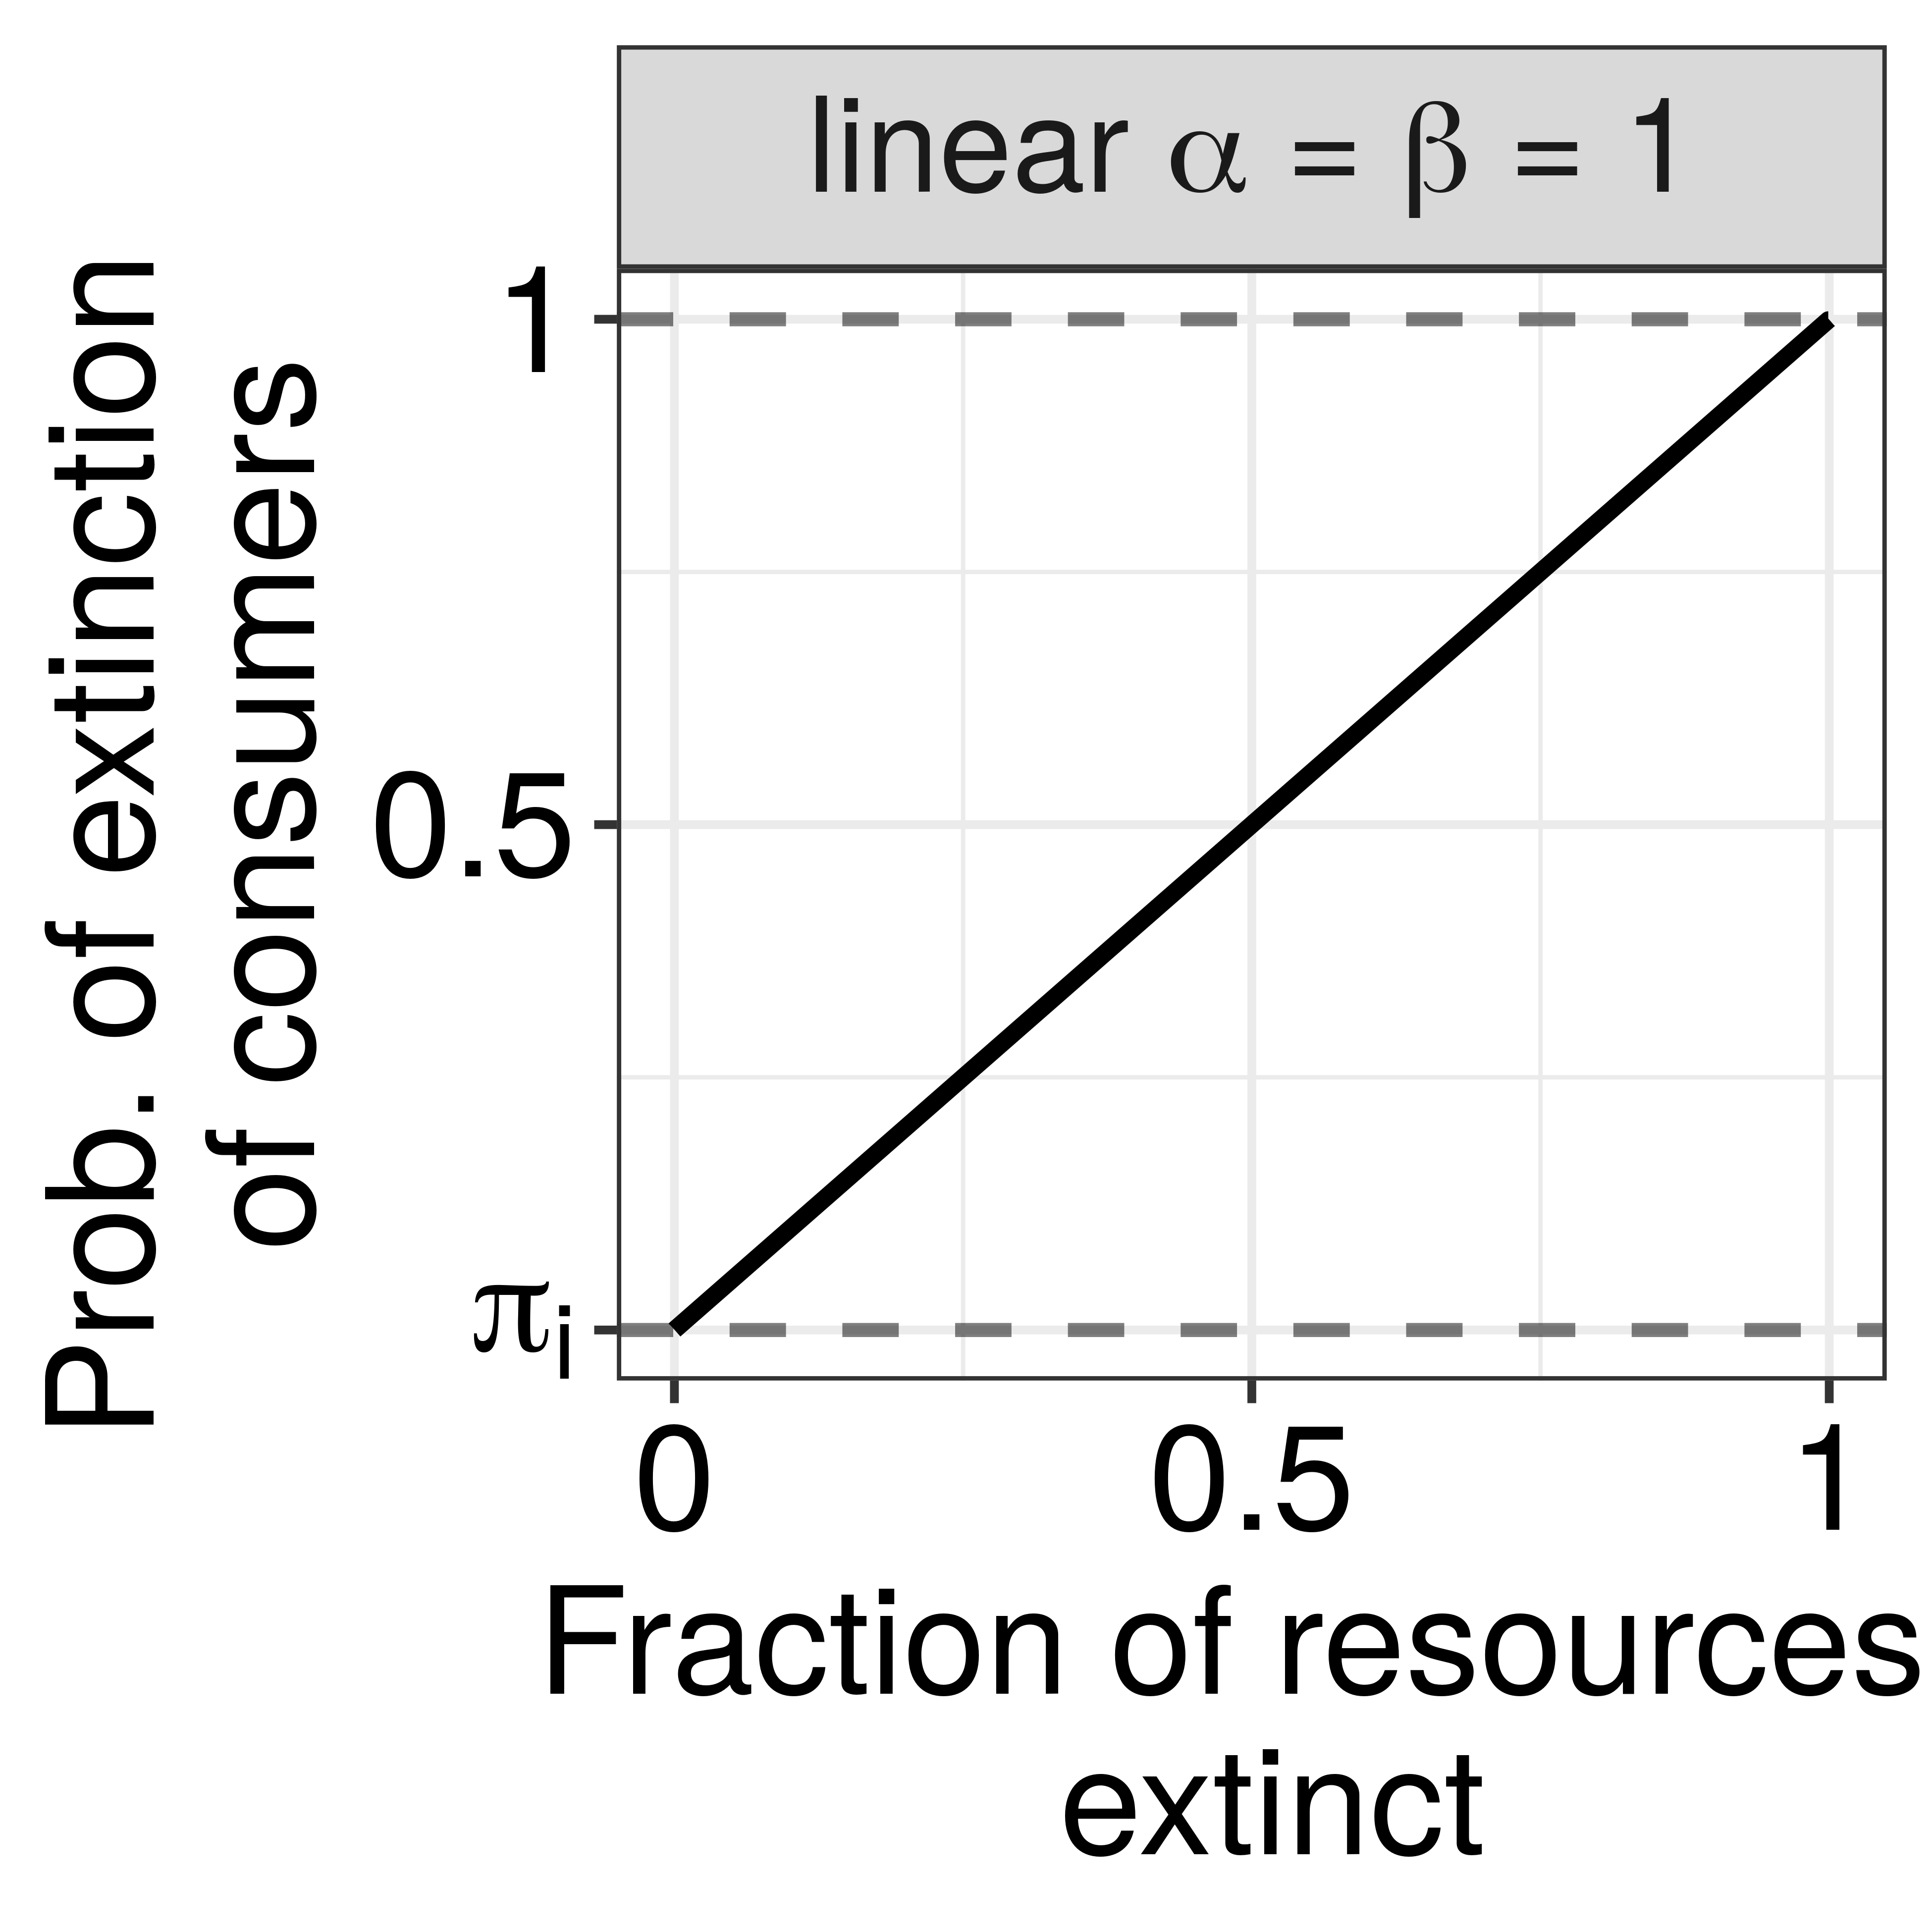
\includegraphics[width=0.19\textwidth,valign=t]{fform_1_1.png}
  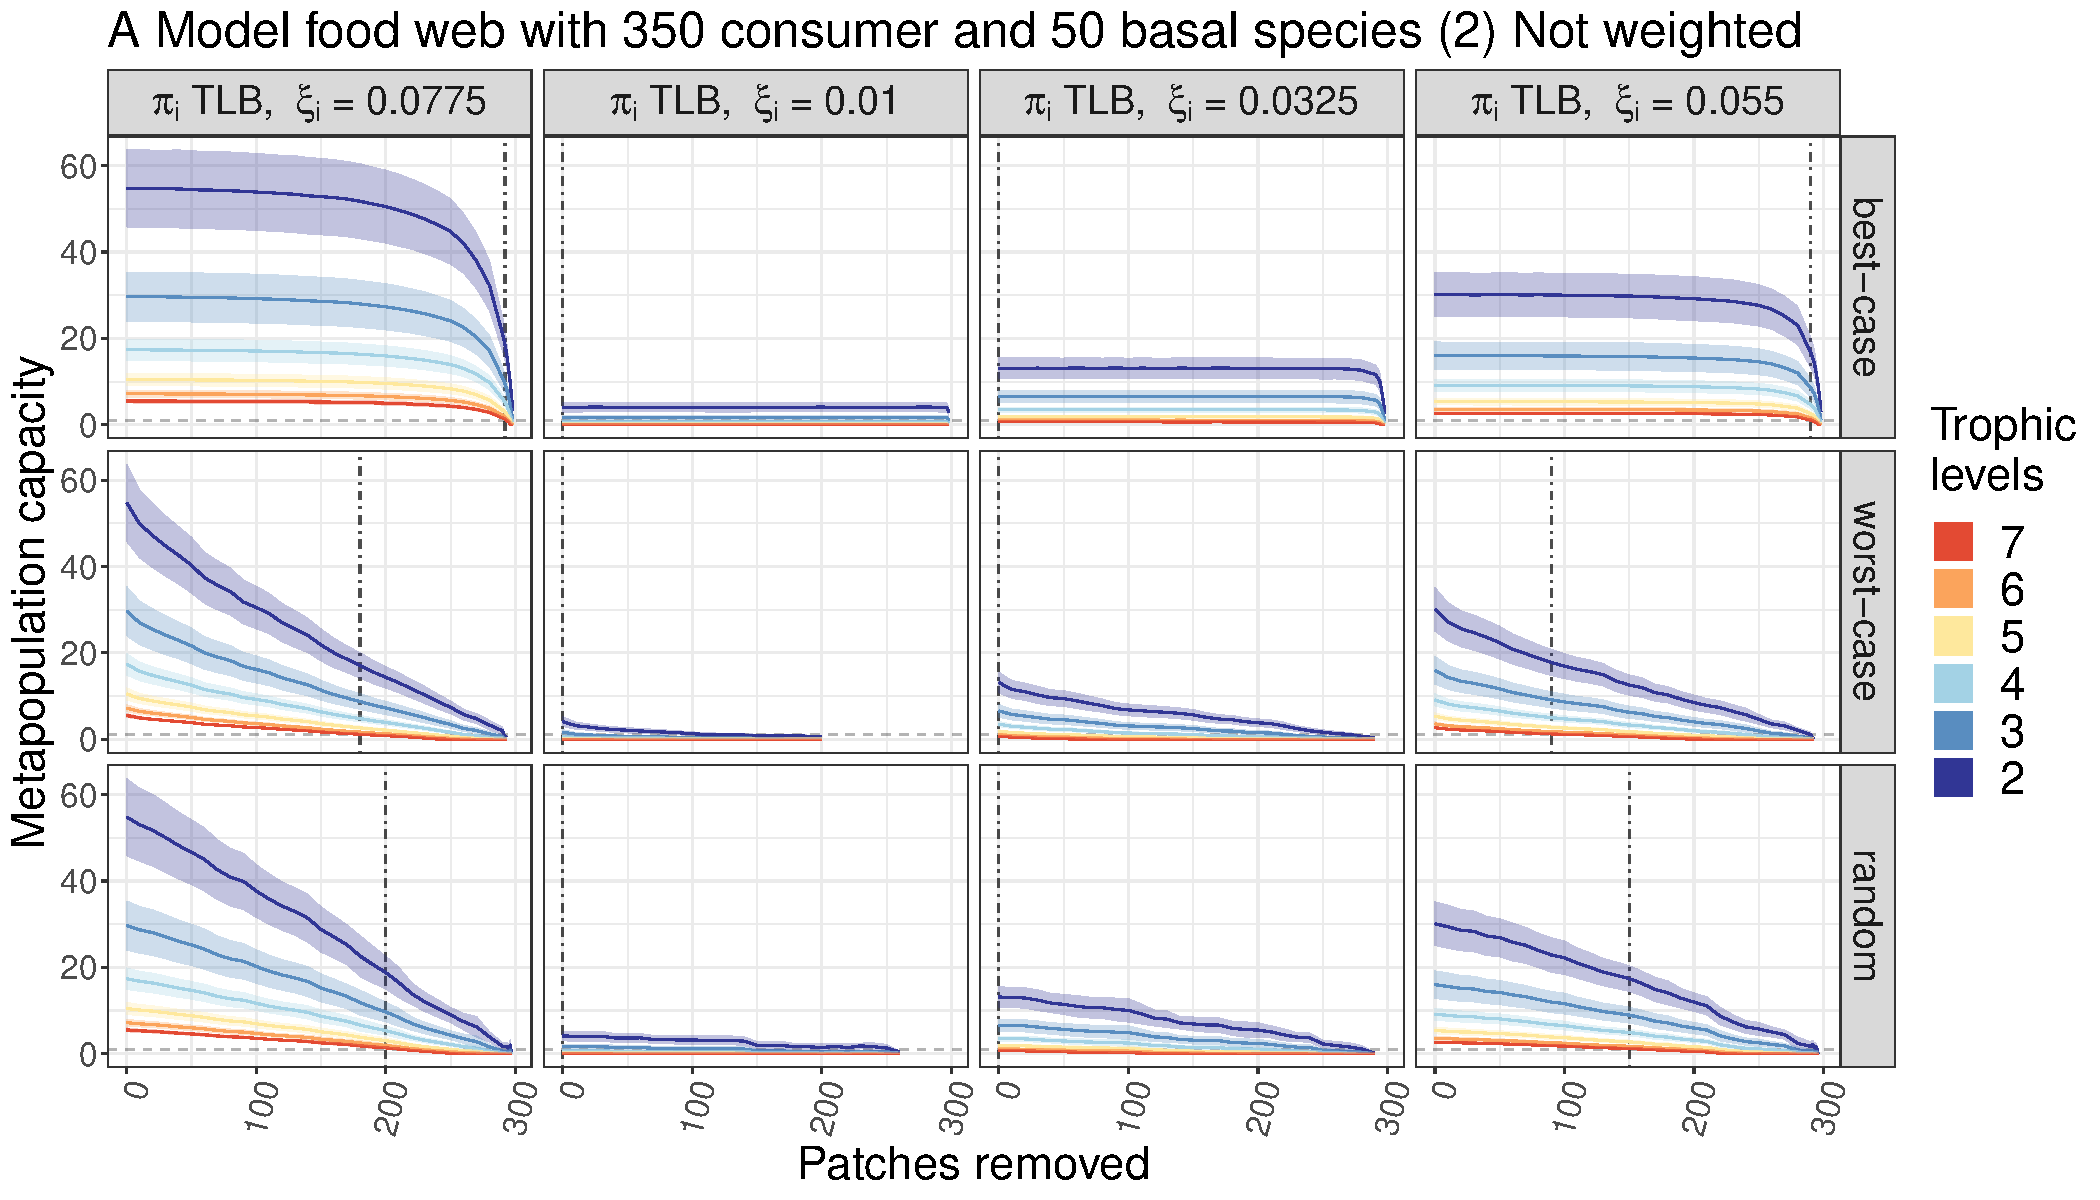
\includegraphics[width=0.8\textwidth,valign=t]{lambda_Model_food_web_with_350_consumer_and_50_basal_species_(2)_Not_weighted_basal_1_1.pdf}
  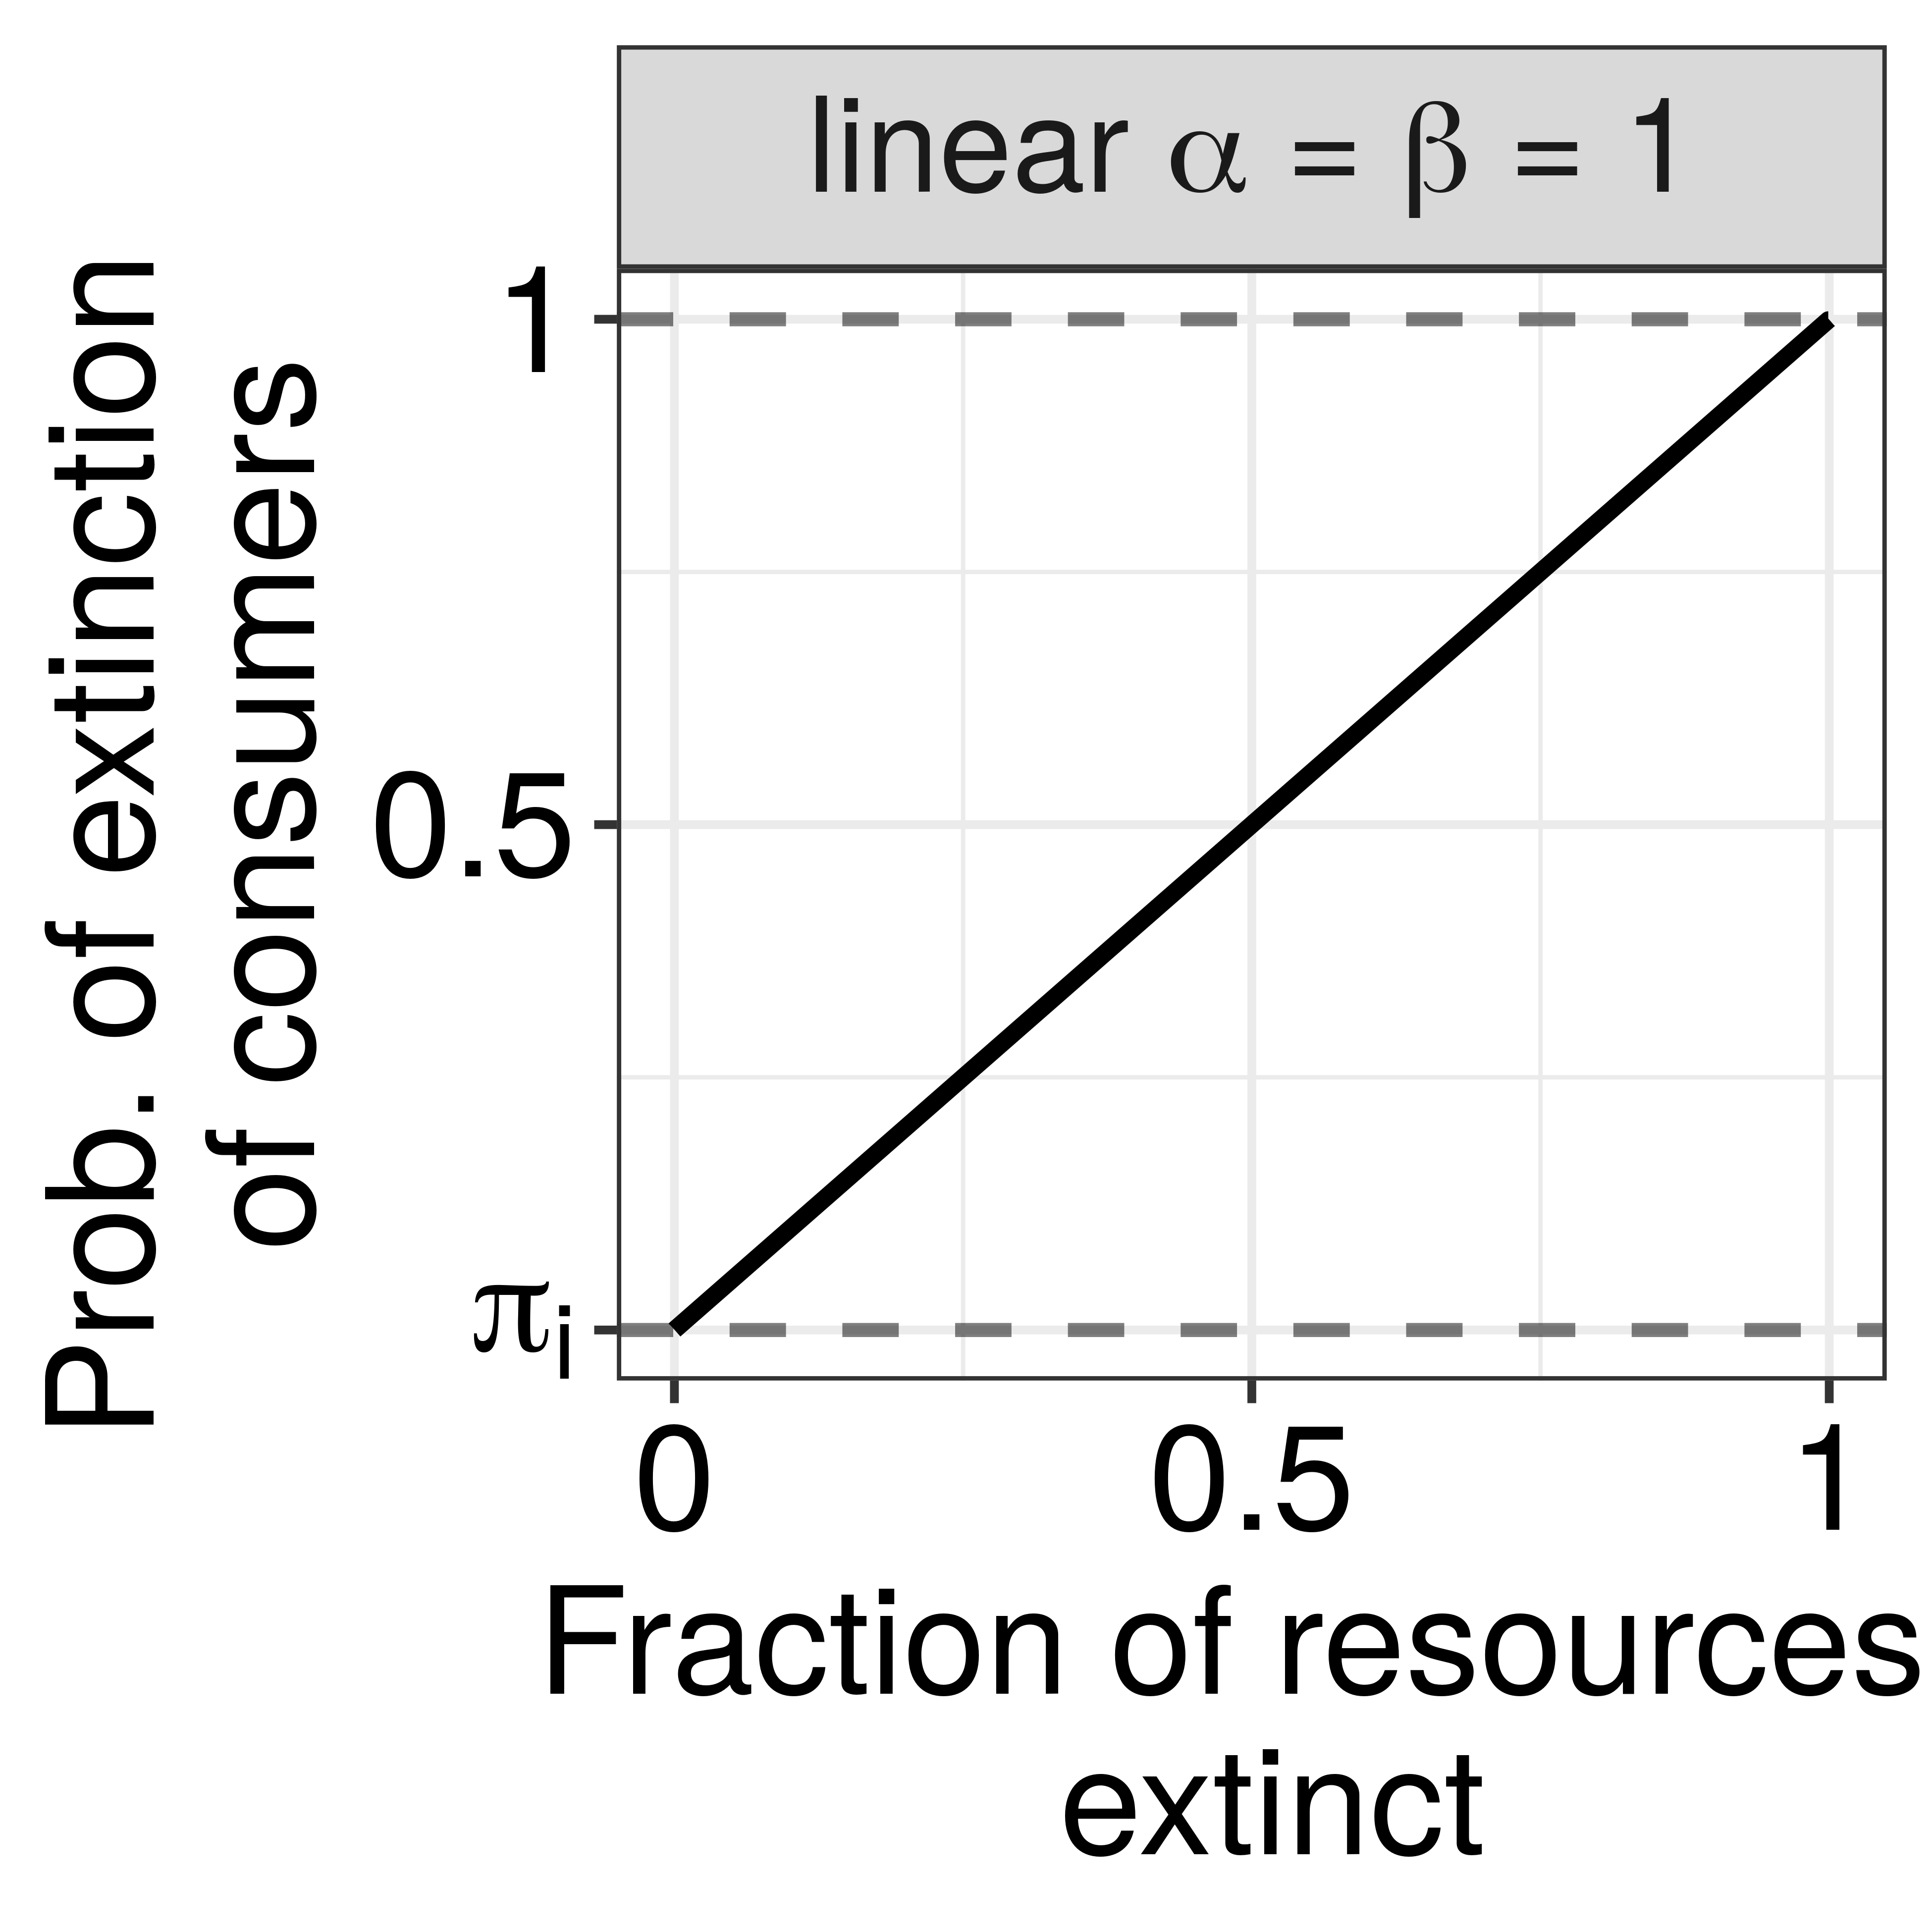
\includegraphics[width=0.19\textwidth,valign=t]{fform_1_1.png}
  \caption{As Figure~\ref{fig:patchloss_web1_11}.}
  \label{fig:patchloss_web2_11}
\end{figure}

\begin{figure}\ContinuedFloat
  \includegraphics[width=0.8\textwidth,valign=t]{lambda_Model_food_web_with_350_consumer_and_50_basal_species_(2)_Weighted_basal_5_1.pdf}
  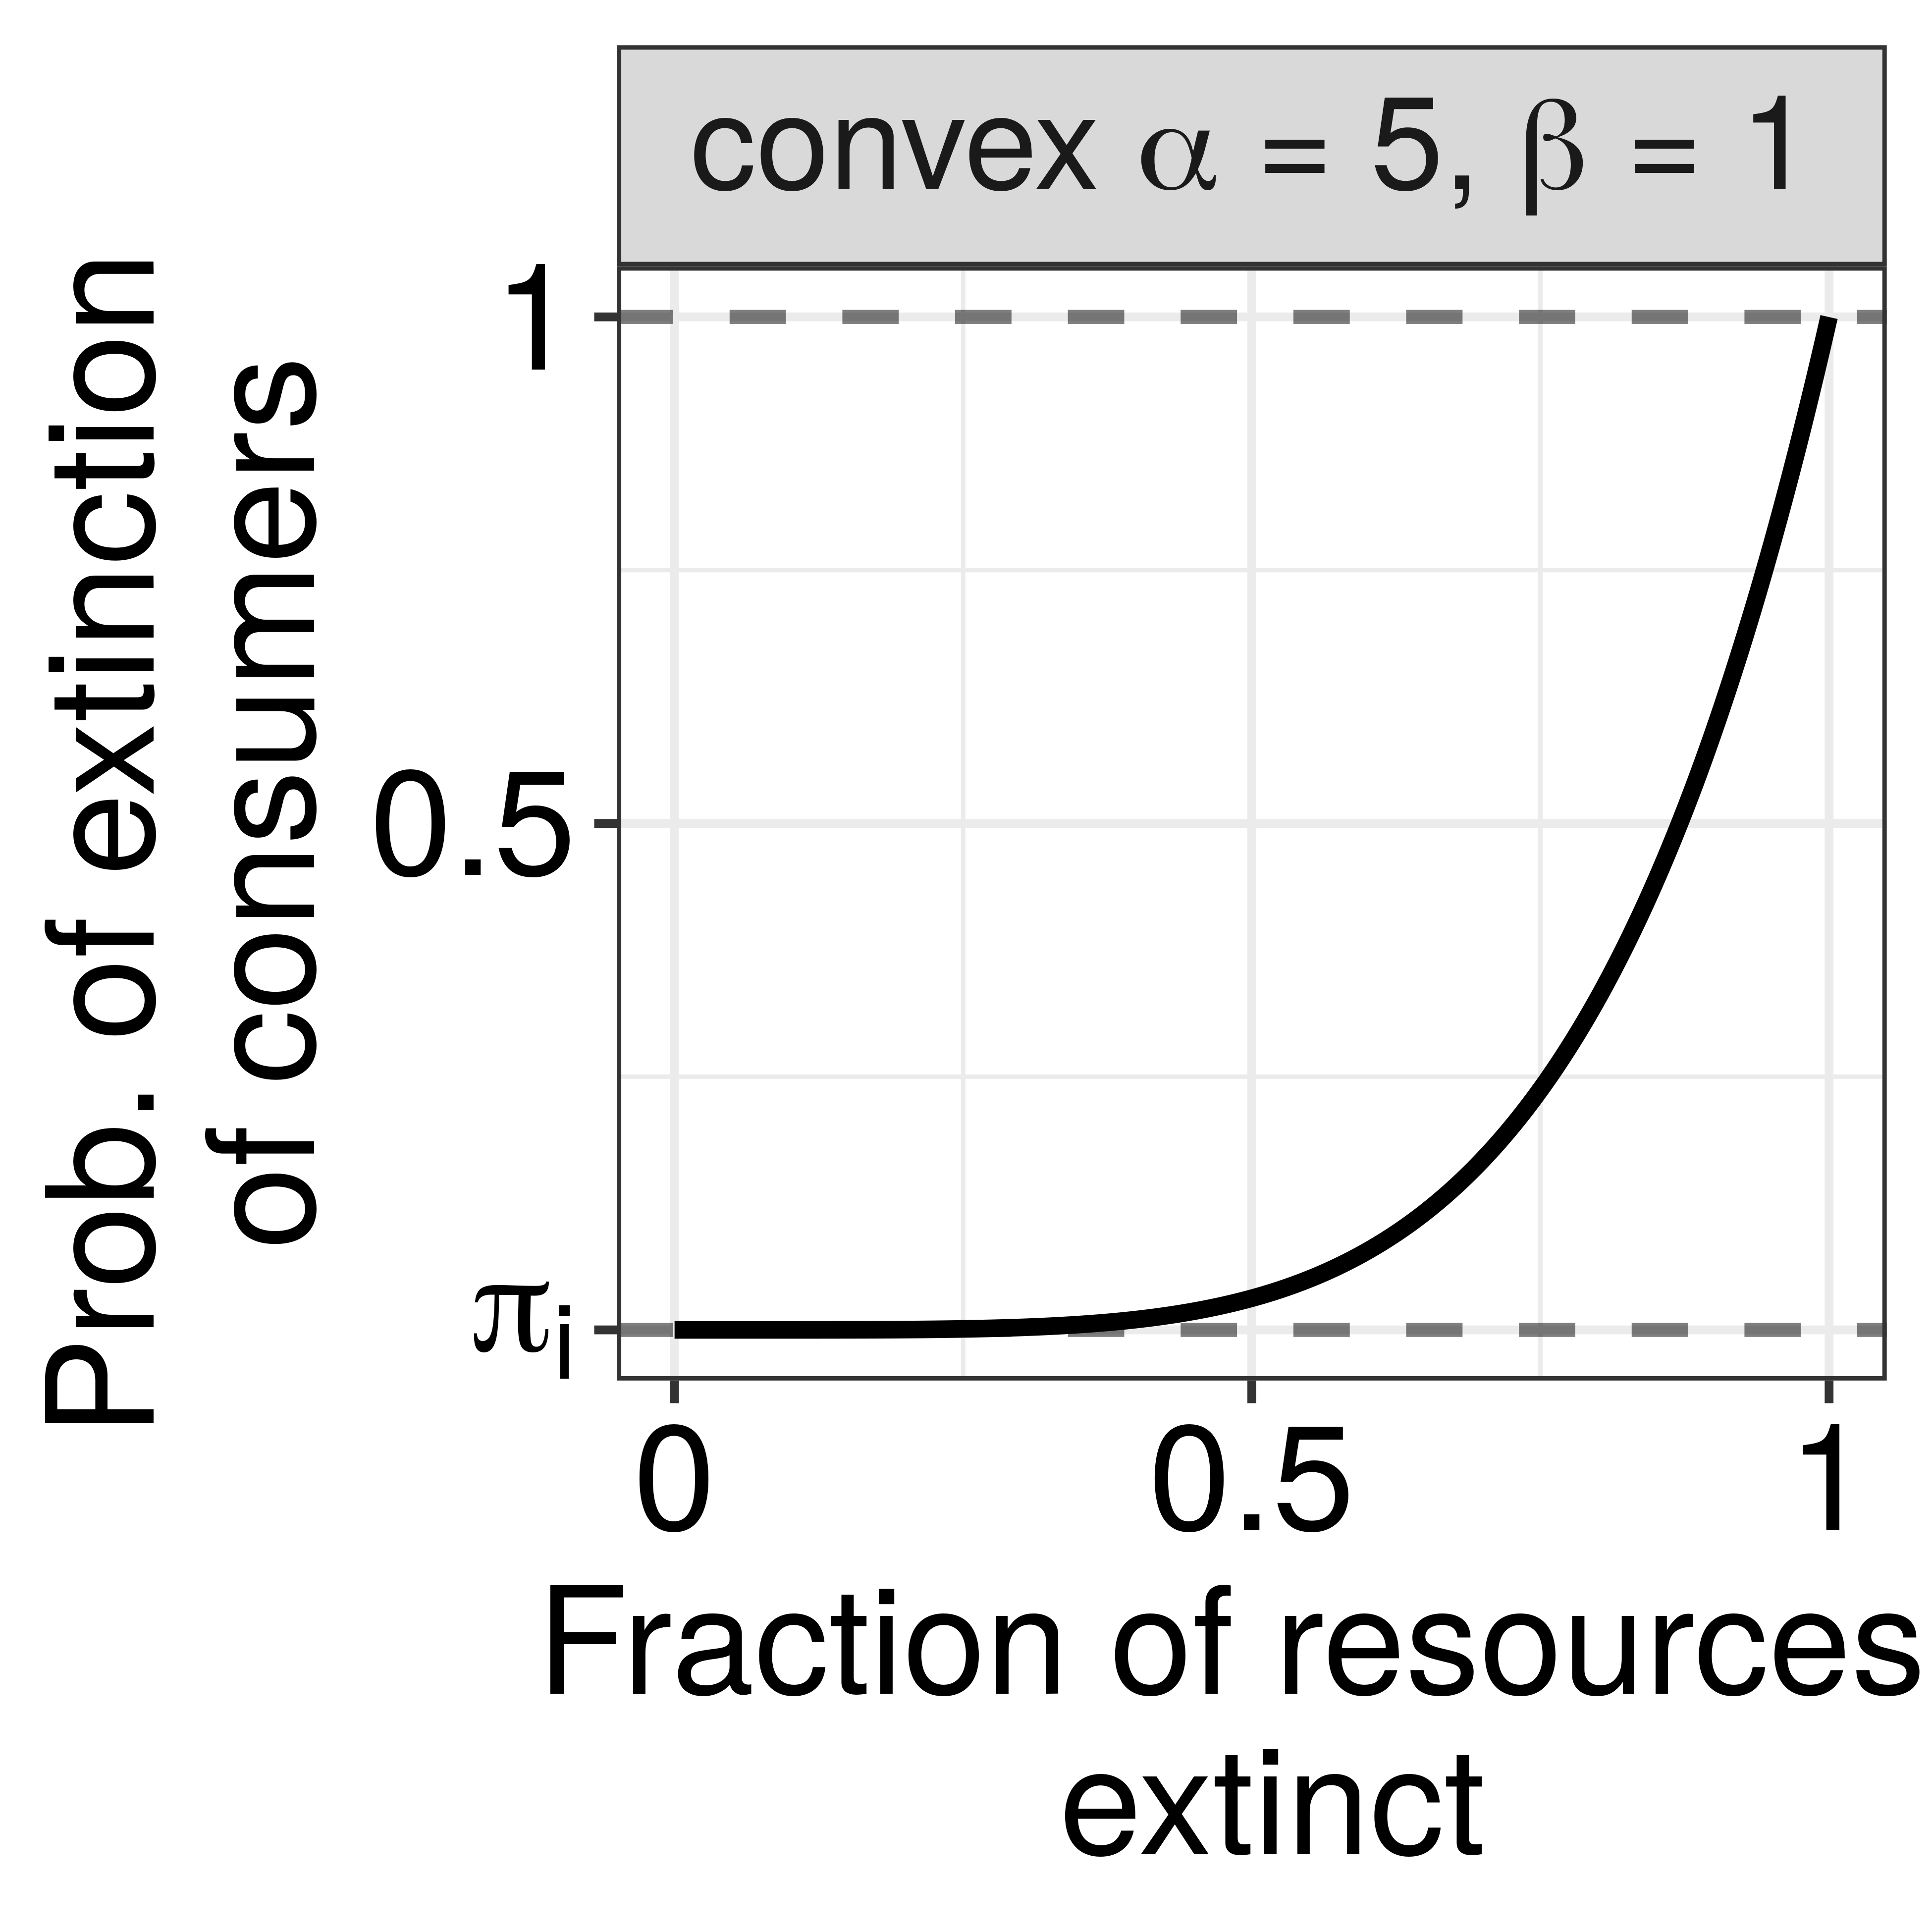
\includegraphics[width=0.19\textwidth,valign=t]{fform_5_1.png}
  \includegraphics[width=0.8\textwidth,valign=t]{lambda_Model_food_web_with_350_consumer_and_50_basal_species_(2)_Not_weighted_basal_5_1.pdf}
  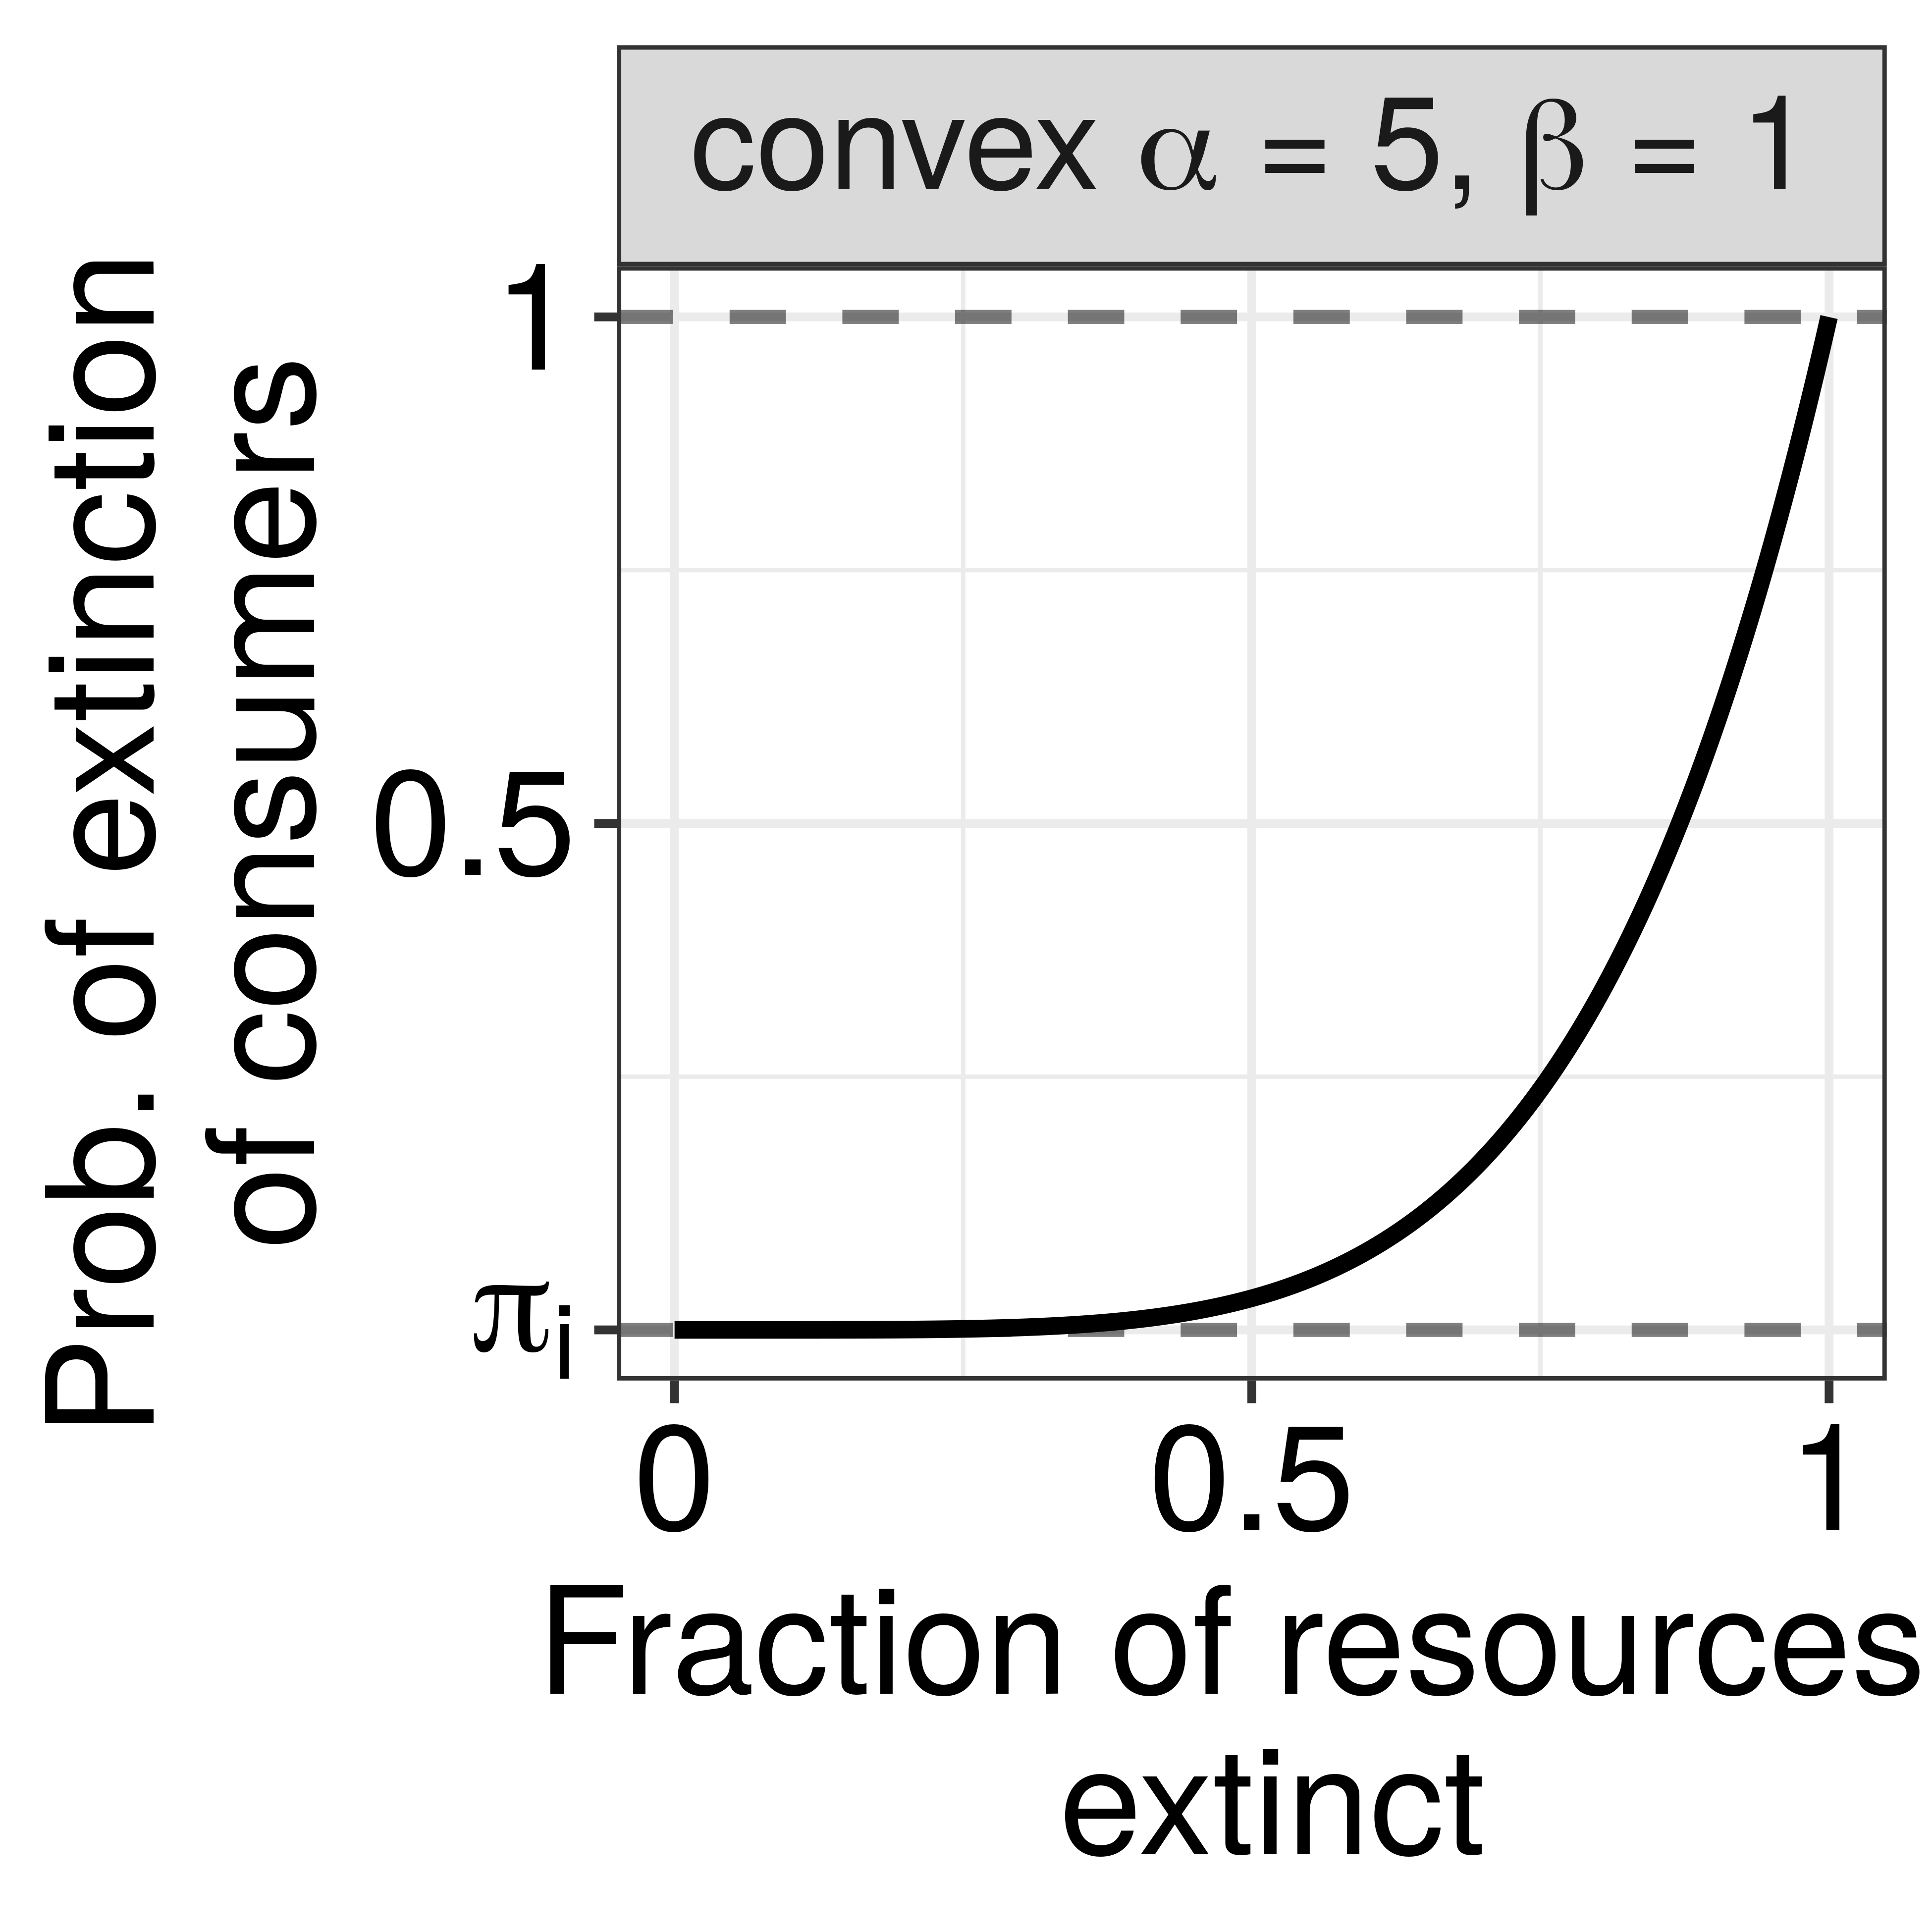
\includegraphics[width=0.19\textwidth,valign=t]{fform_5_1.png}
  \caption{Figure continued.}
  \label{fig:patchloss_web2_51}
\end{figure}

\begin{figure}\ContinuedFloat
  \includegraphics[width=0.8\textwidth,valign=t]{lambda_Model_food_web_with_350_consumer_and_50_basal_species_(2)_Weighted_basal_1_5.pdf}
  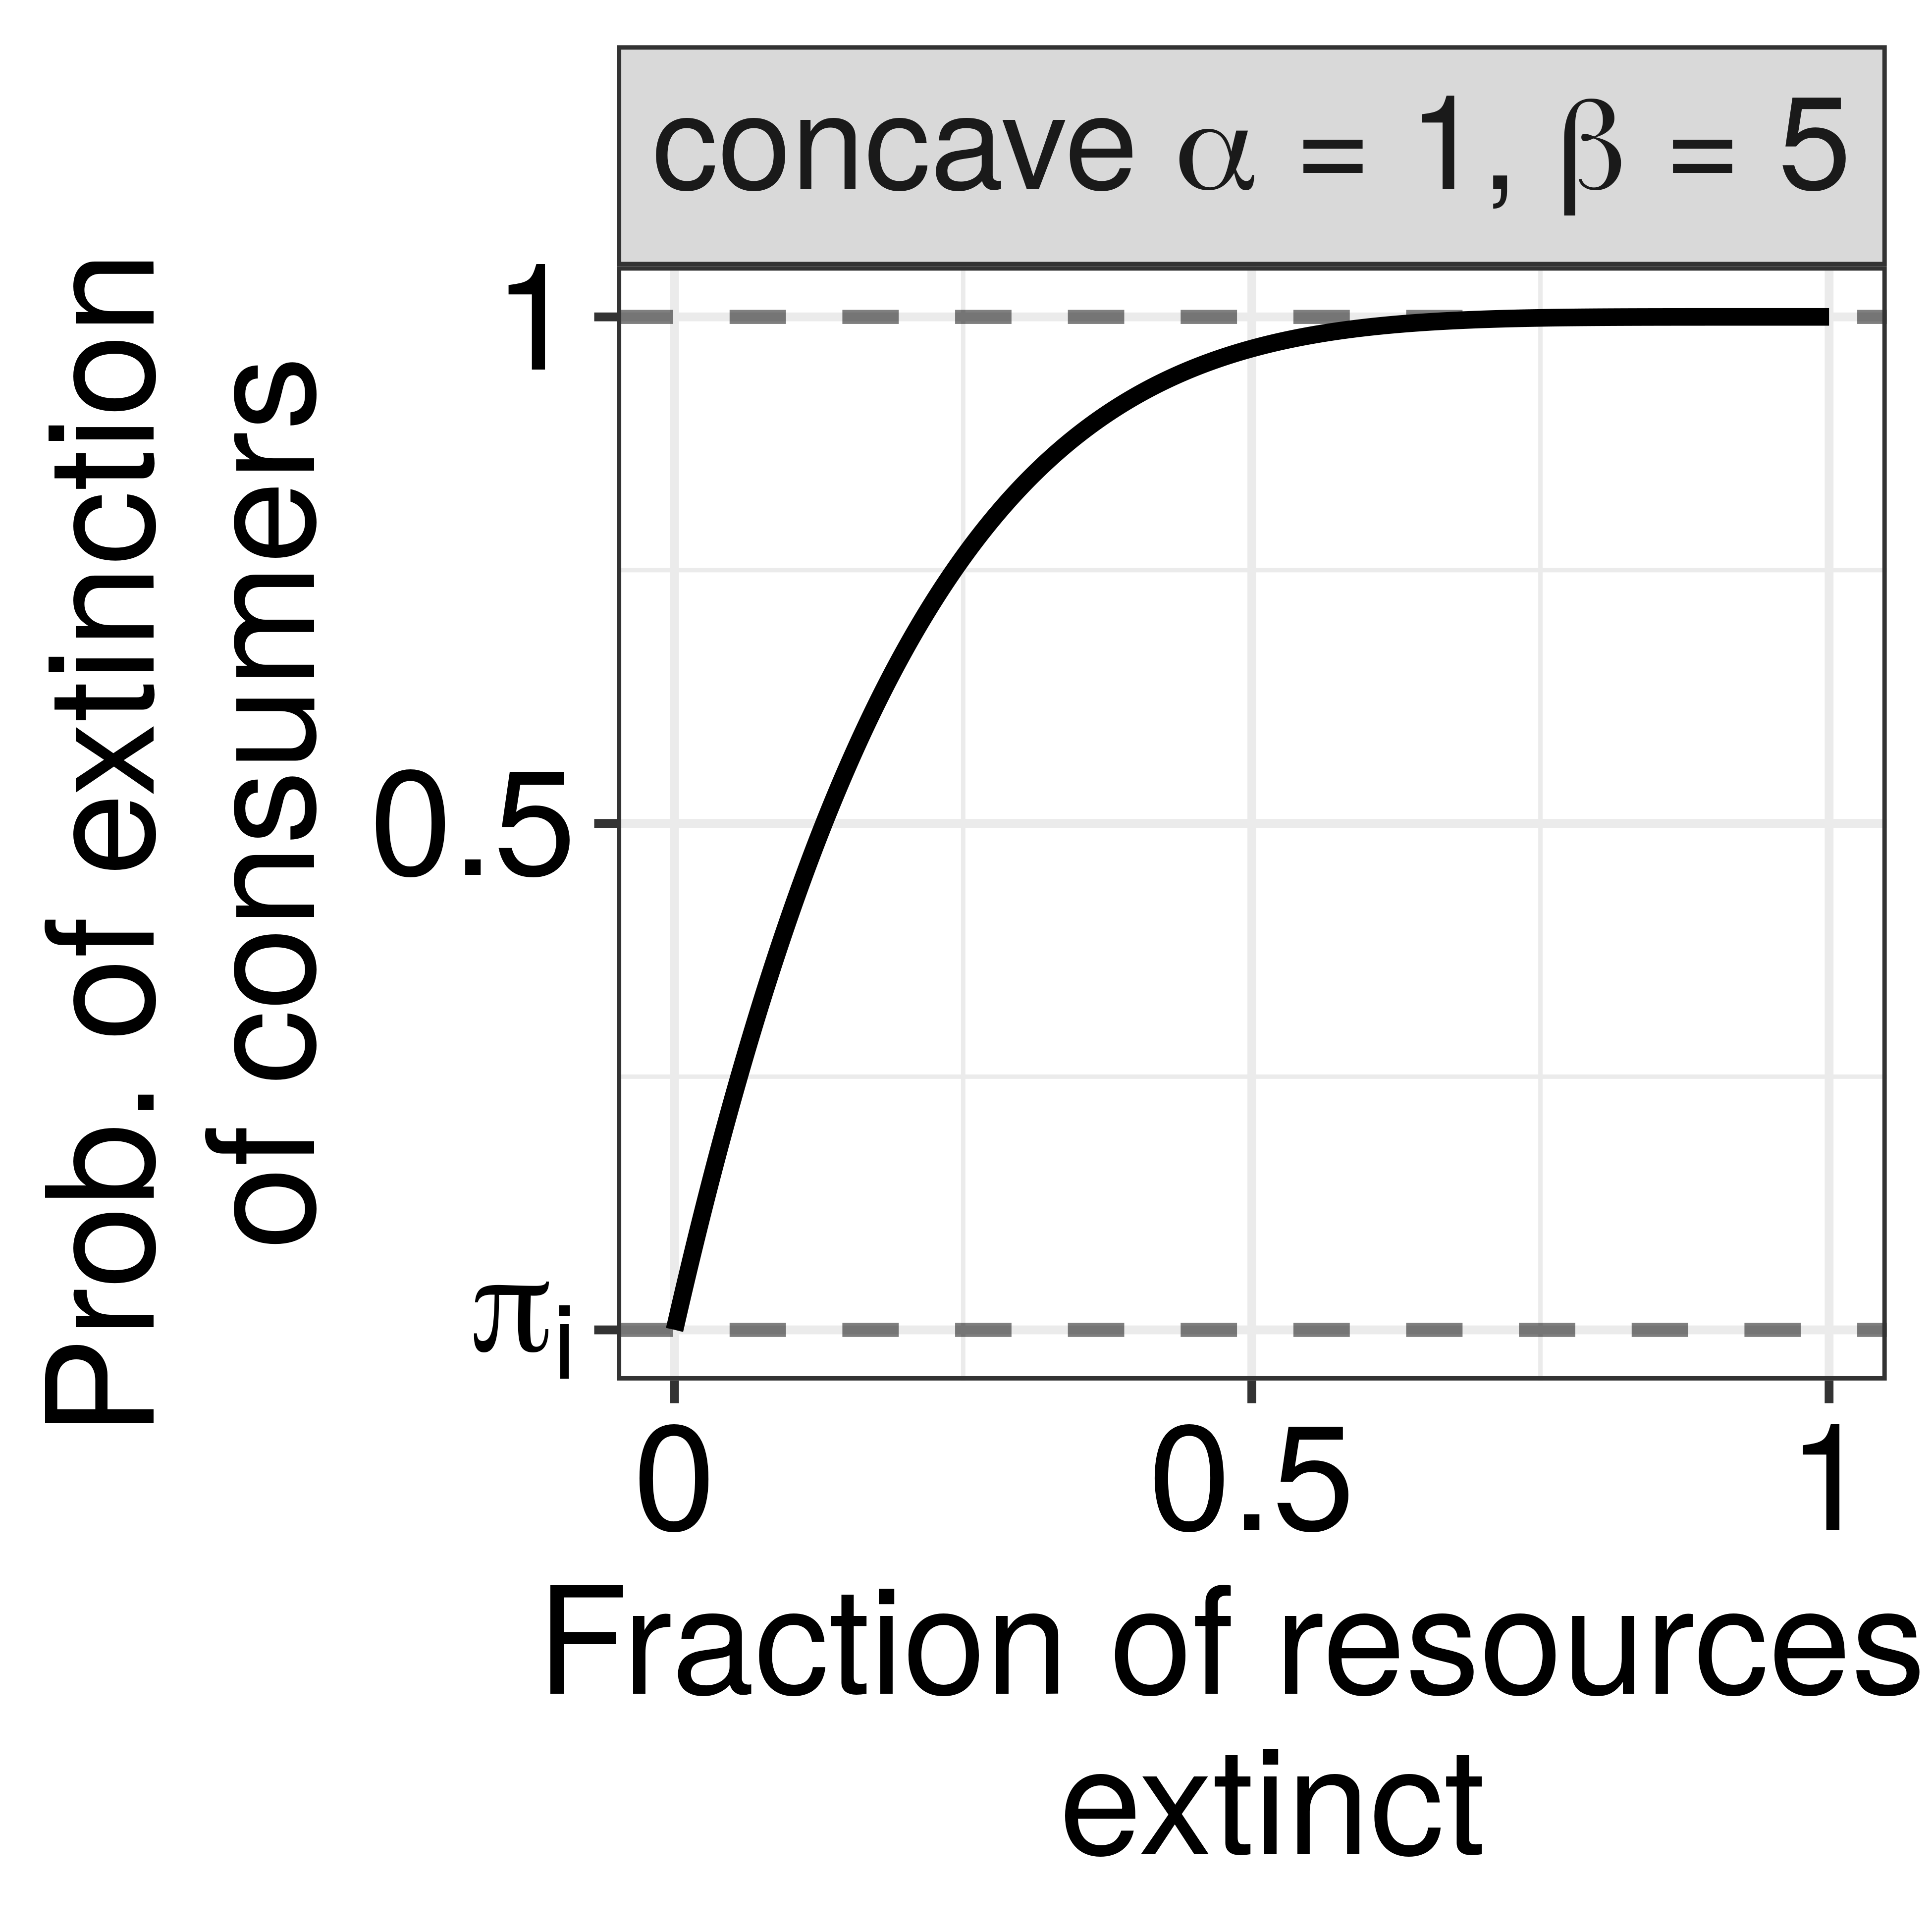
\includegraphics[width=0.19\textwidth,valign=t]{fform_1_5.png}
  \includegraphics[width=0.8\textwidth,valign=t]{lambda_Model_food_web_with_350_consumer_and_50_basal_species_(2)_Not_weighted_basal_1_5.pdf}
  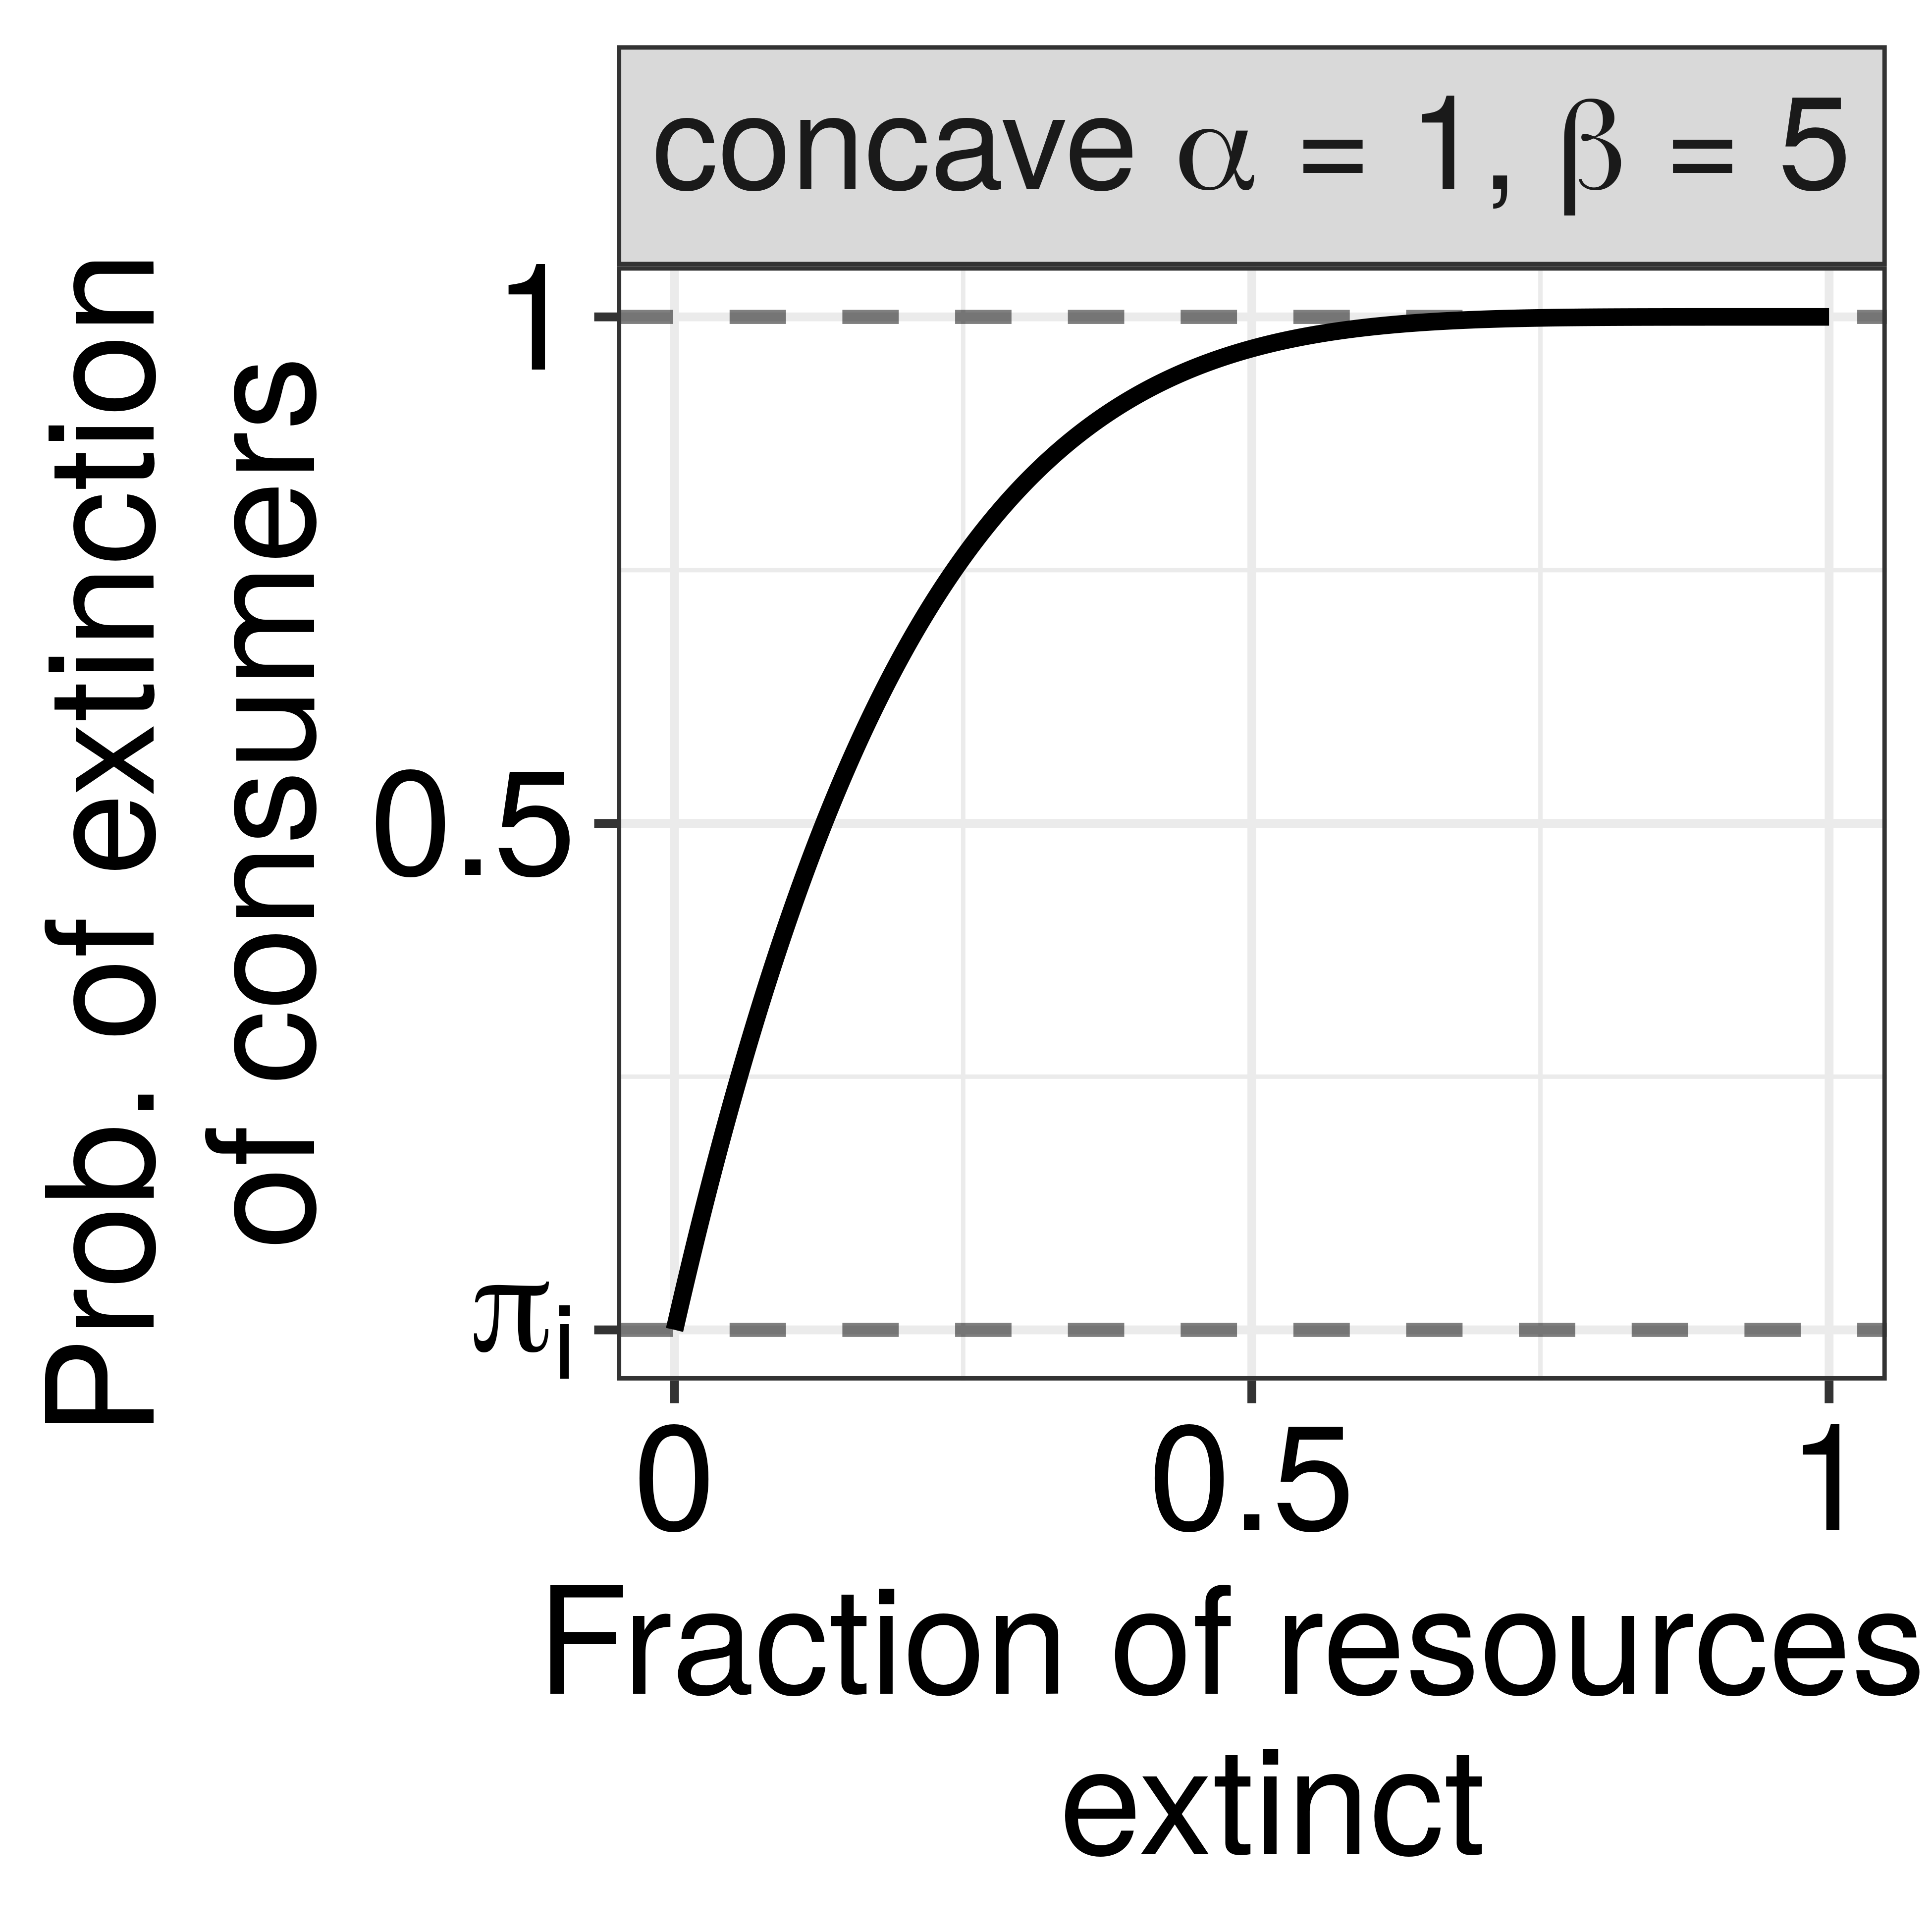
\includegraphics[width=0.19\textwidth,valign=t]{fform_1_5.png}
  \caption{Figure continued.}
  \label{fig:patchloss_web2_15}
\end{figure}

\begin{figure}\ContinuedFloat
  \includegraphics[width=0.8\textwidth,valign=t]{lambda_Model_food_web_with_350_consumer_and_50_basal_species_(2)_Weighted_basal_5_5.pdf}
  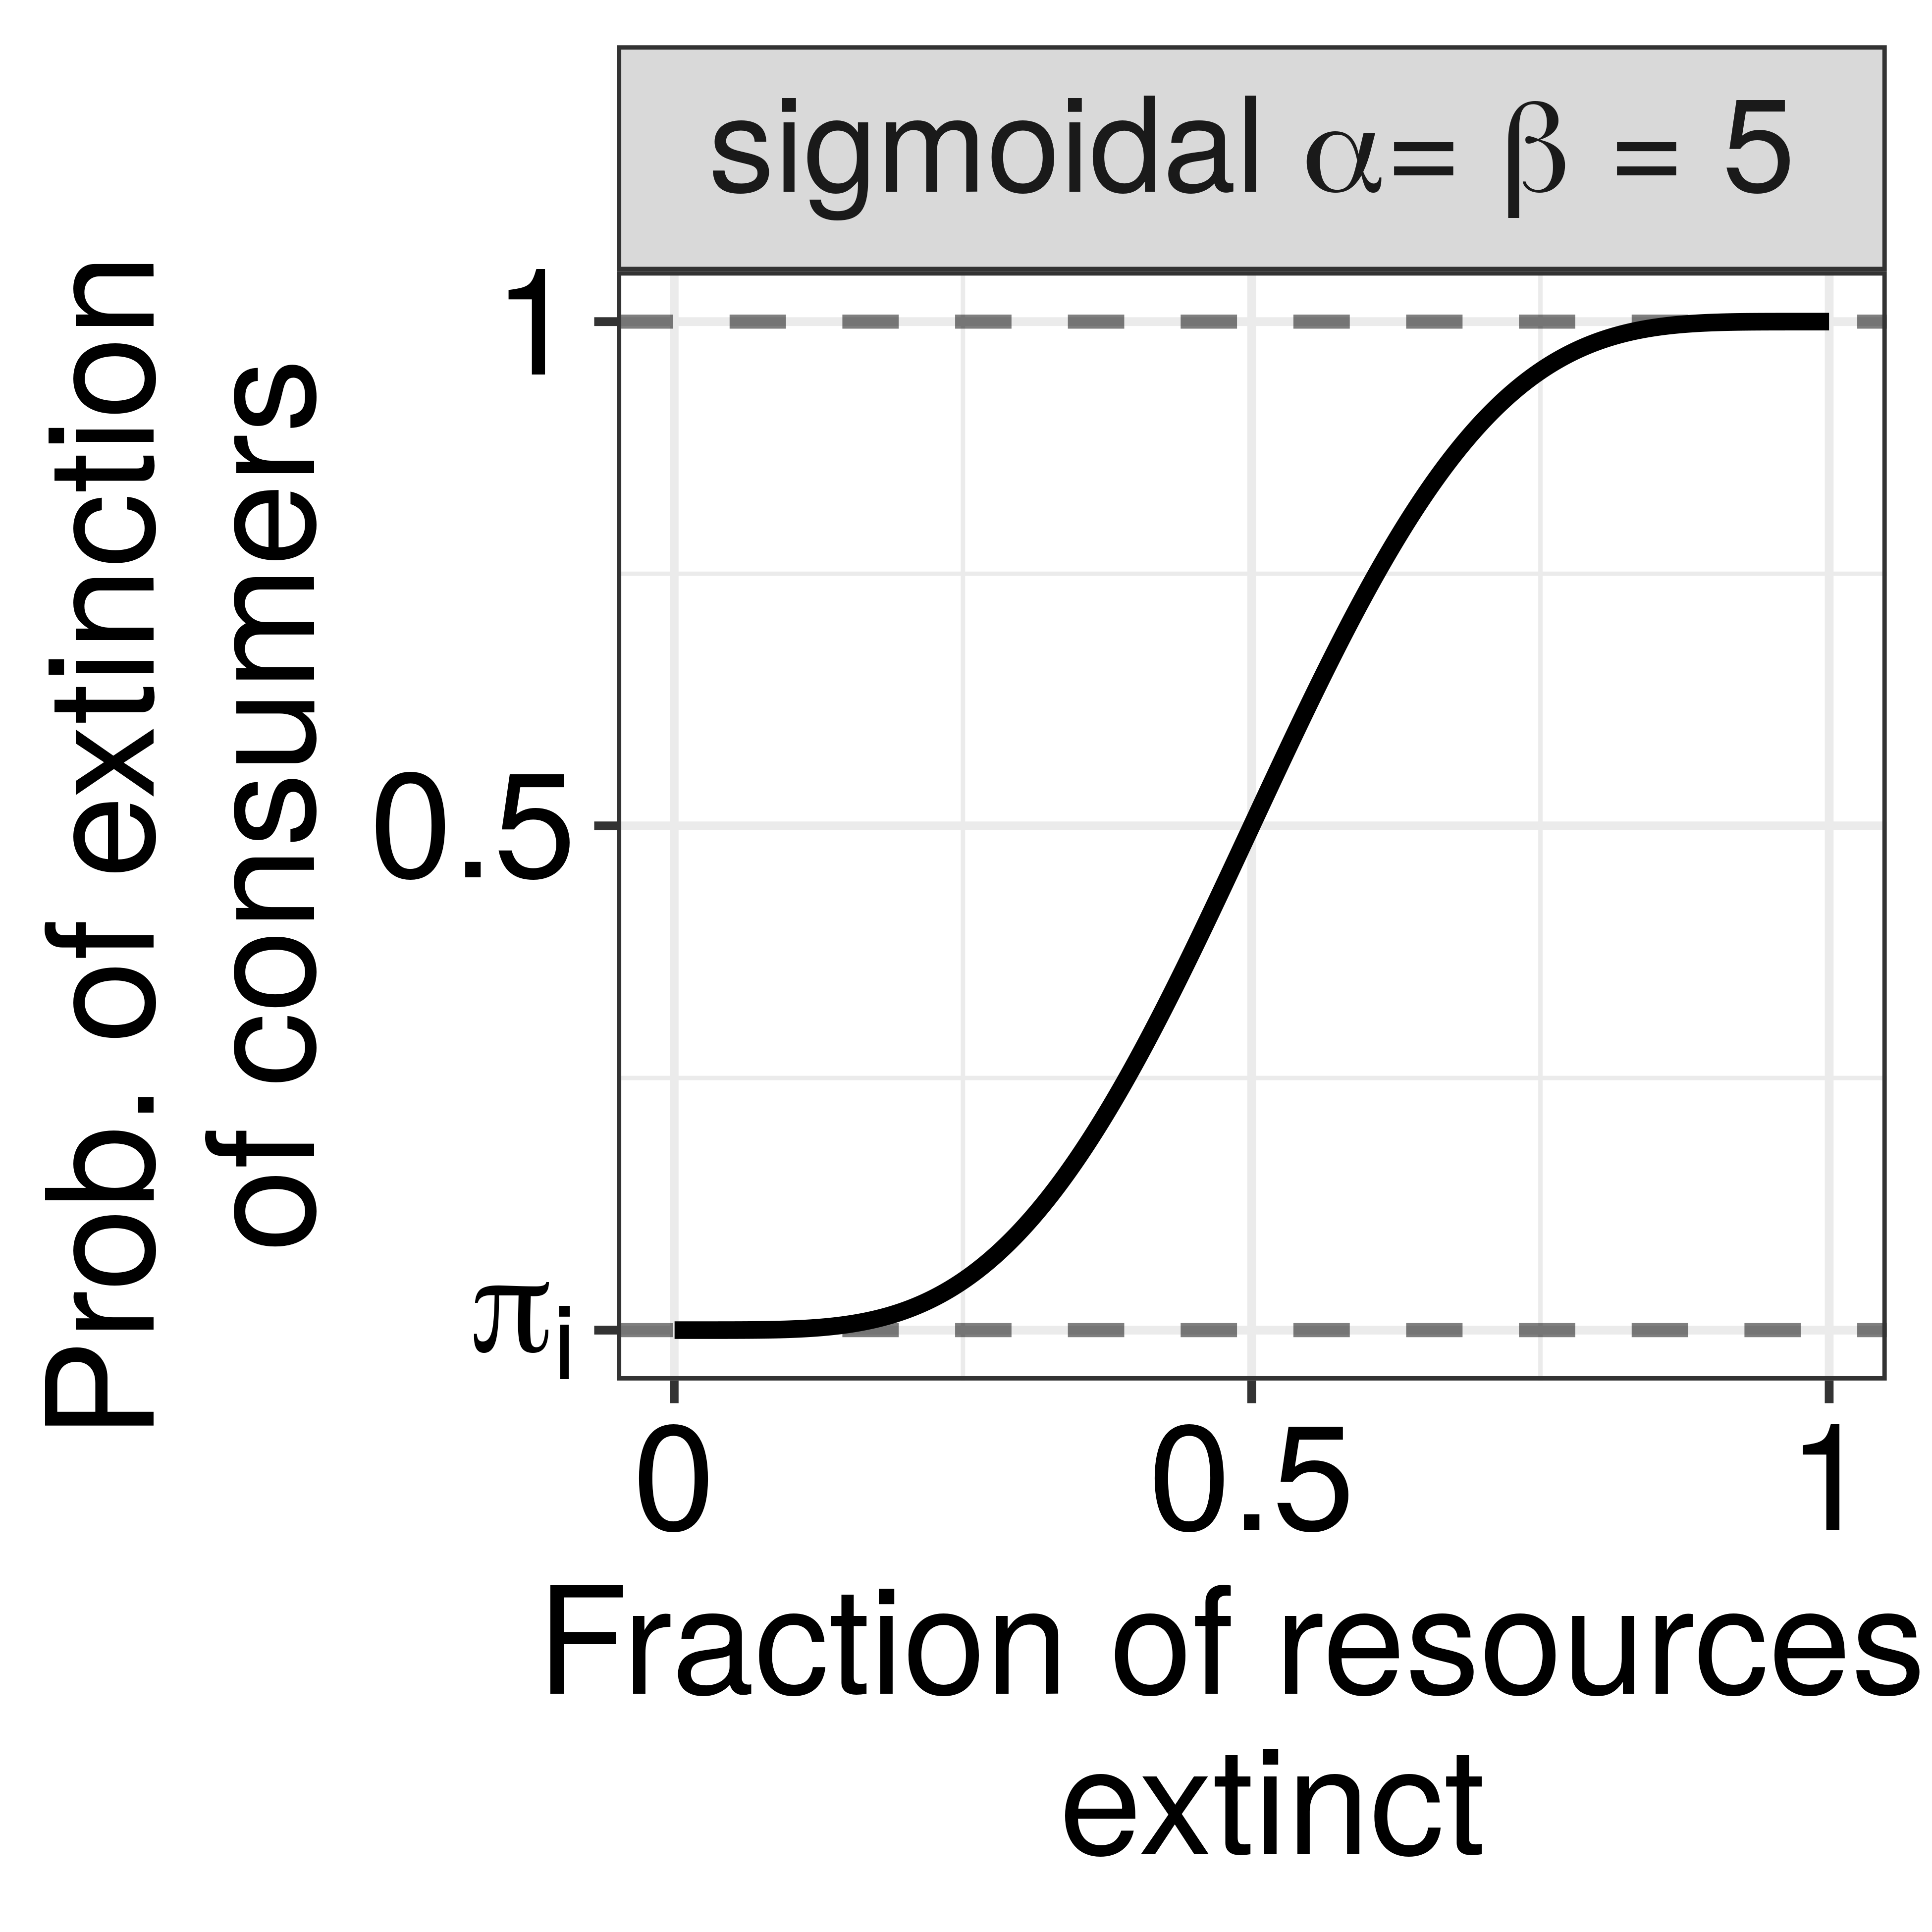
\includegraphics[width=0.19\textwidth,valign=t]{fform_5_5.png}
  \includegraphics[width=0.8\textwidth,valign=t]{lambda_Model_food_web_with_350_consumer_and_50_basal_species_(2)_Not_weighted_basal_5_5.pdf}
  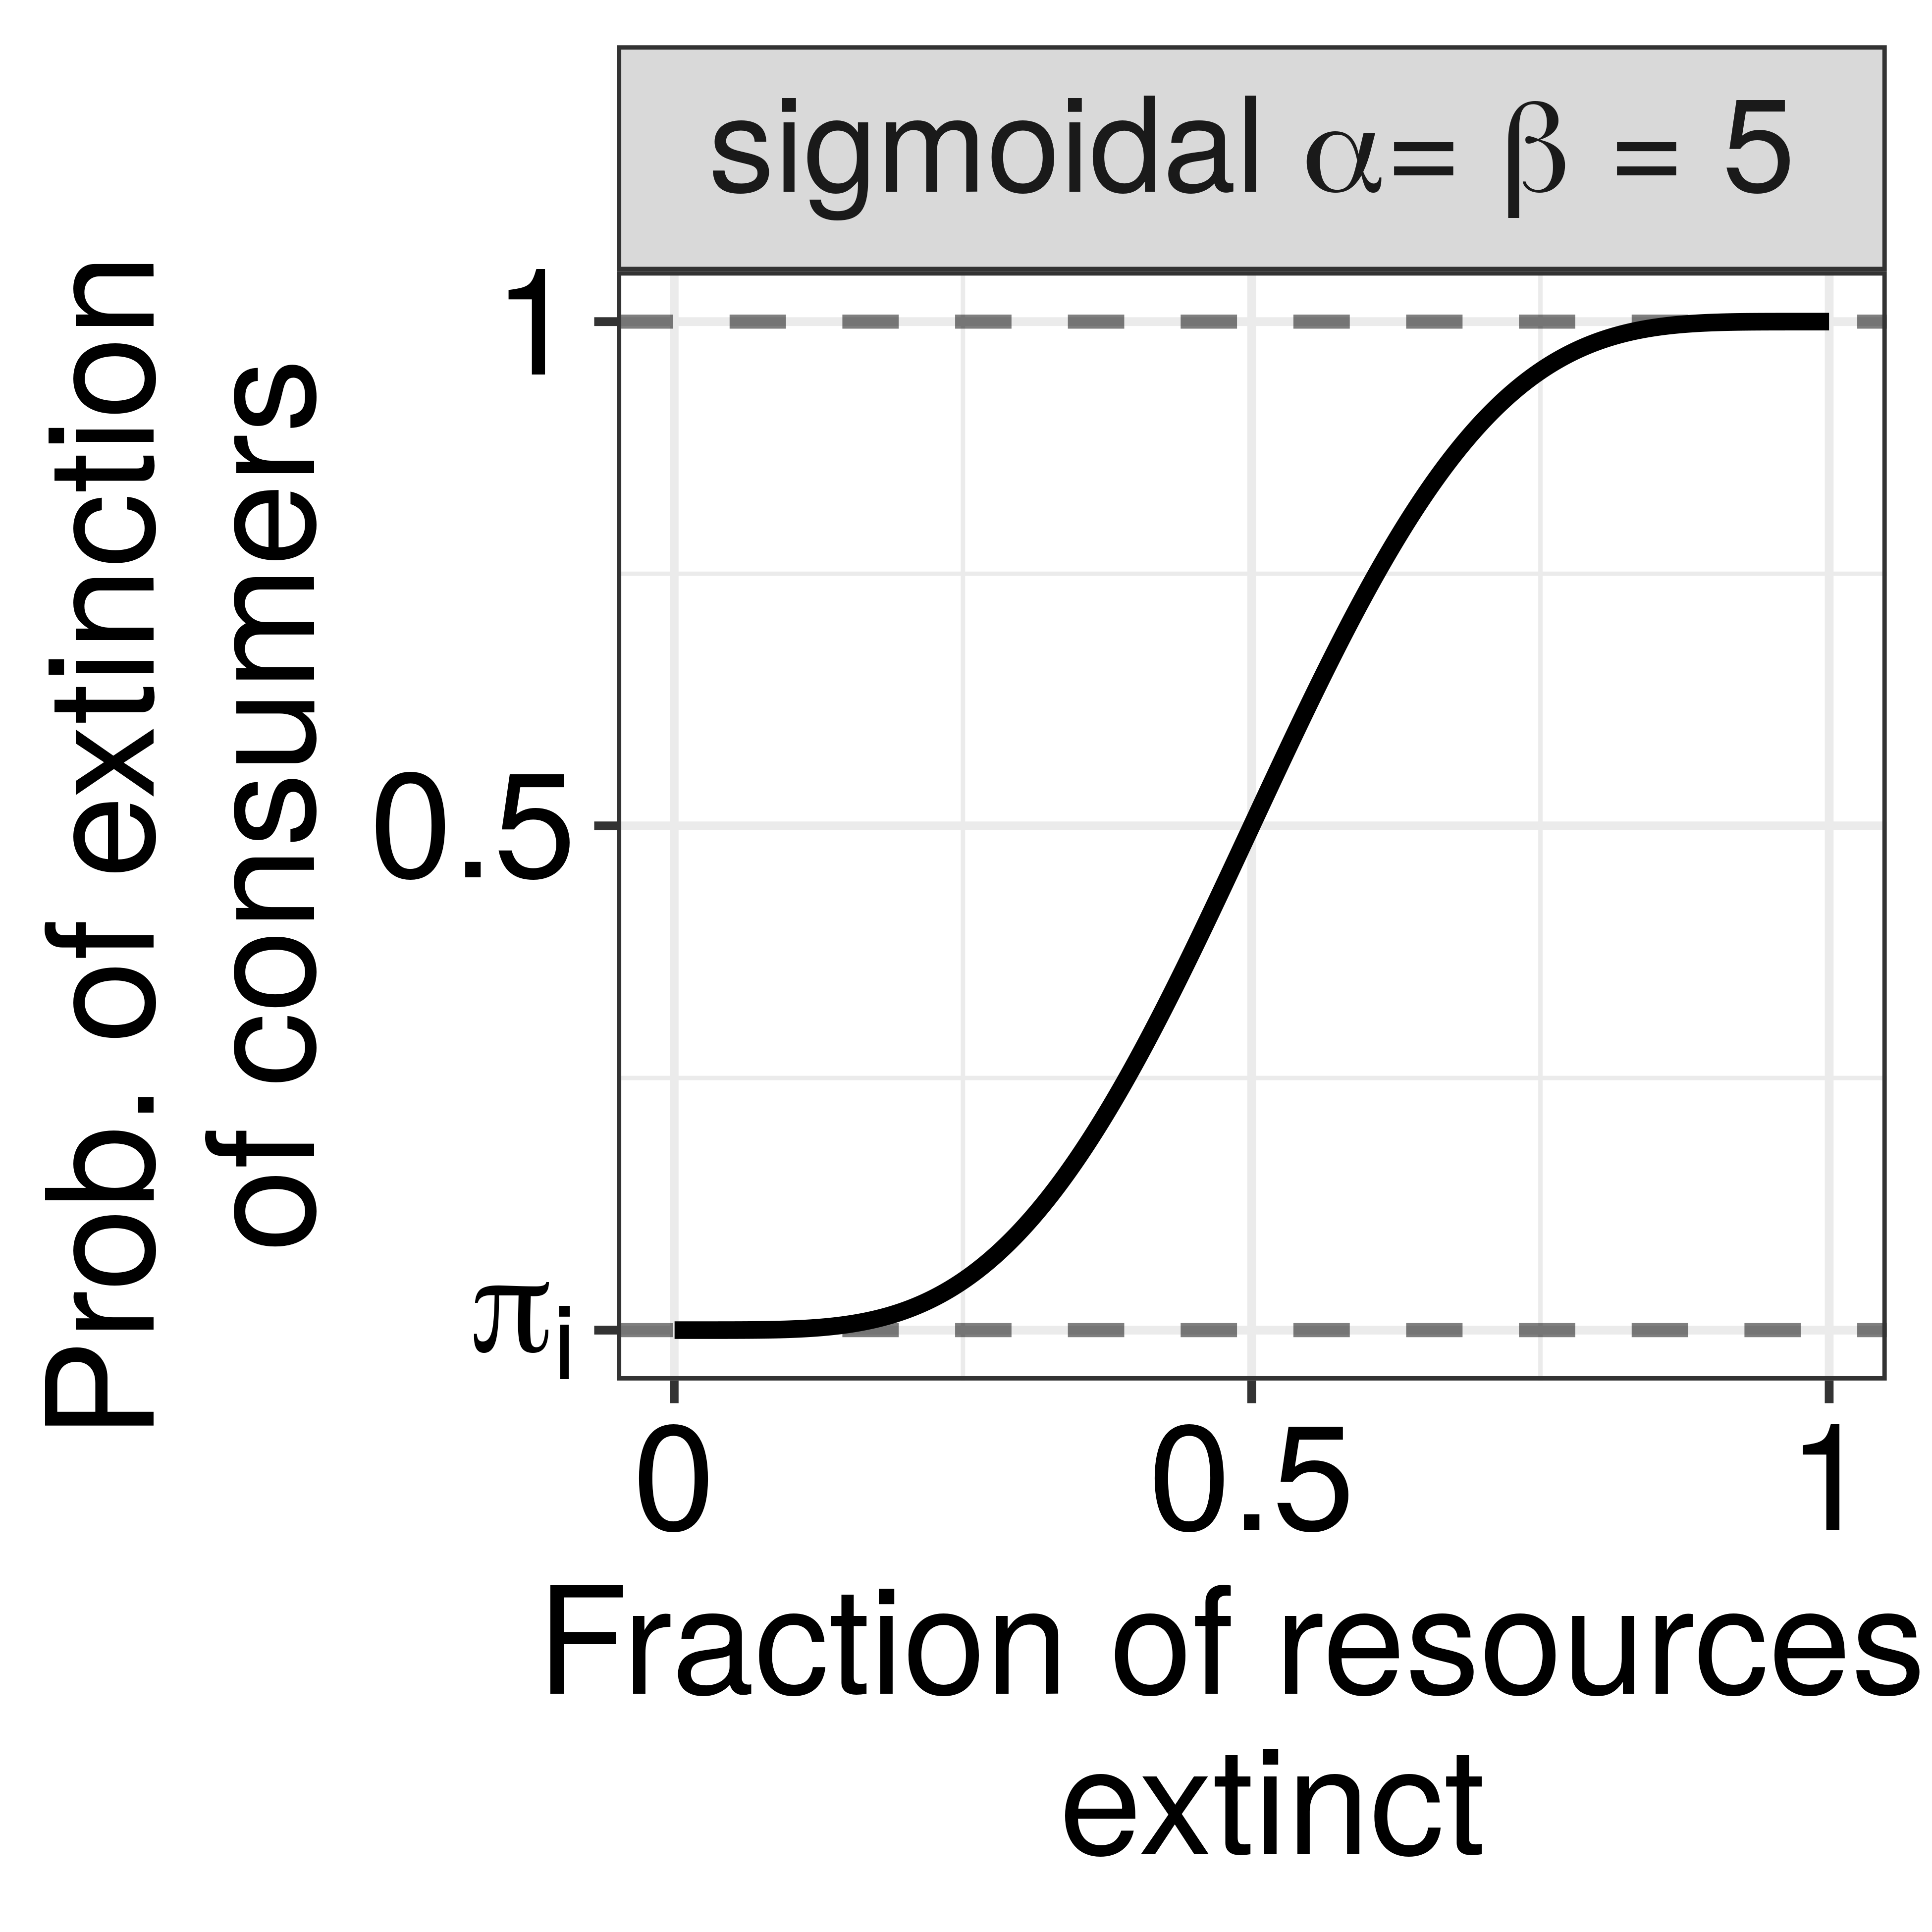
\includegraphics[width=0.19\textwidth,valign=t]{fform_5_5.png}
  \caption{Figure continued.}
  \label{fig:patchloss_web2_55}
\end{figure}

\begin{figure}
  \includegraphics[width=0.8\textwidth,valign=t]{lambda_Model_food_web_with_350_consumer_and_50_basal_species_(3)_Weighted_basal_1_1.pdf}
  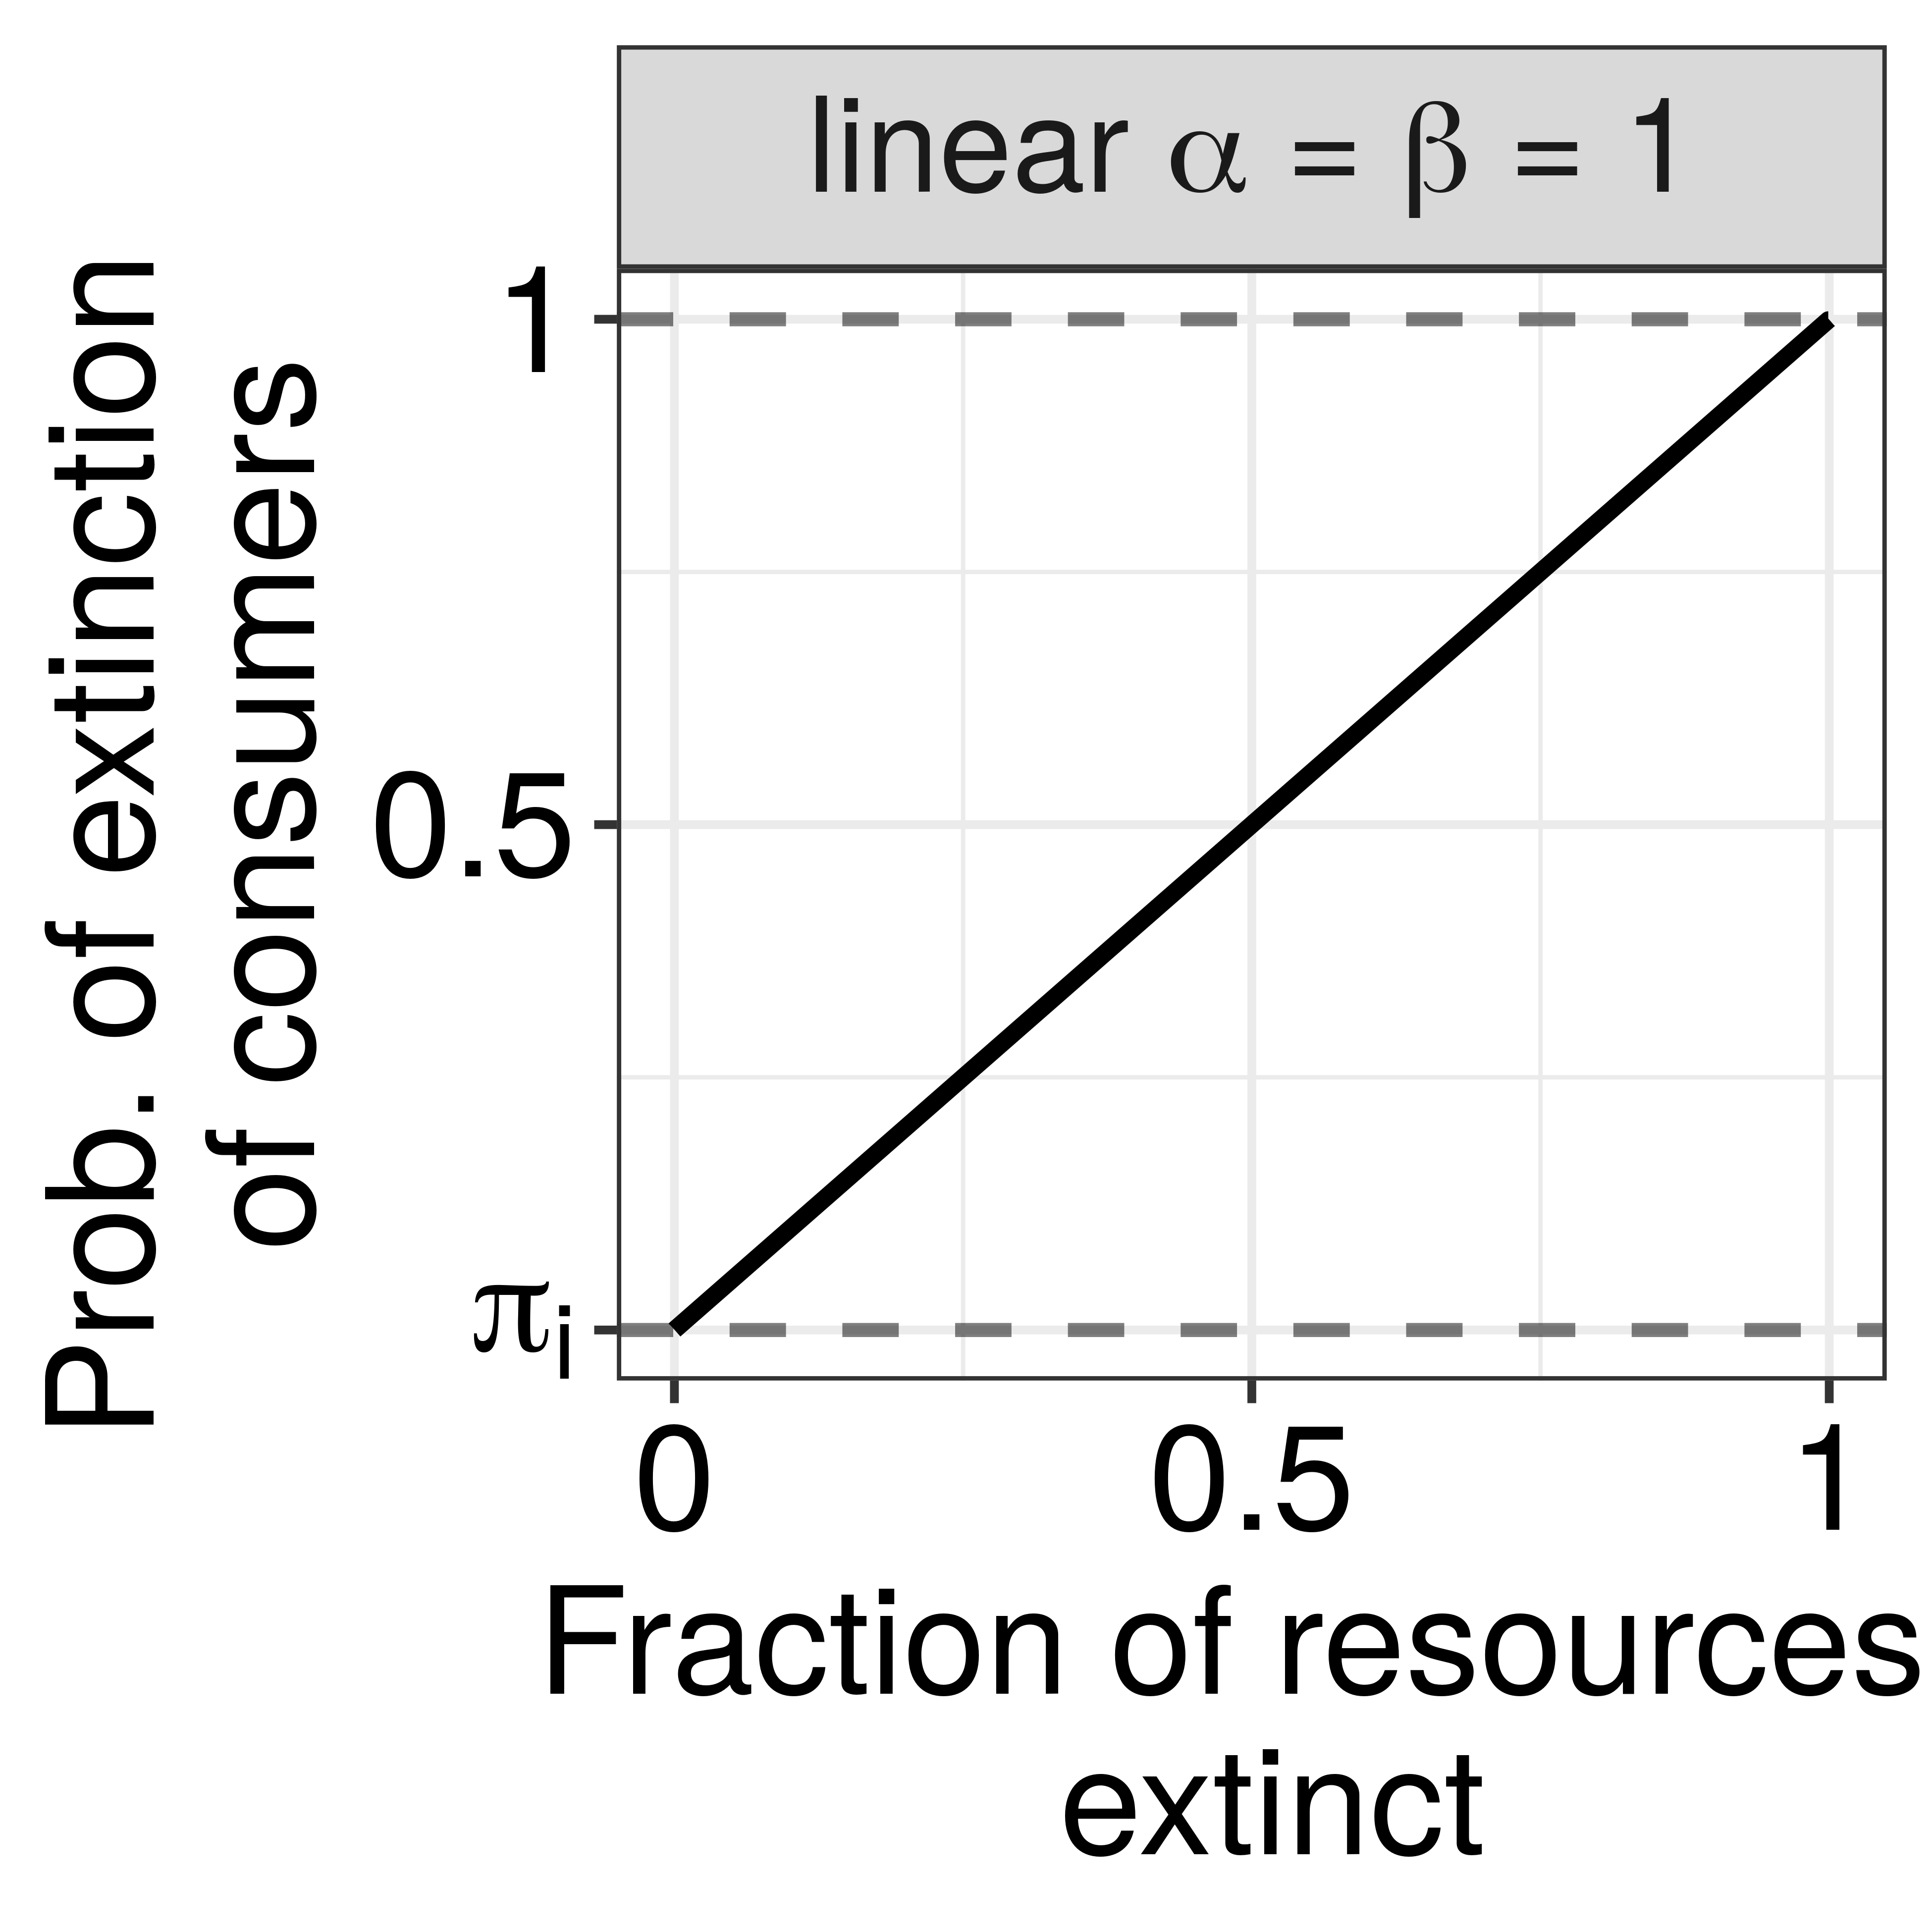
\includegraphics[width=0.19\textwidth,valign=t]{fform_1_1.png}
  \includegraphics[width=0.8\textwidth,valign=t]{lambda_Model_food_web_with_350_consumer_and_50_basal_species_(3)_Not_weighted_basal_1_1.pdf}
  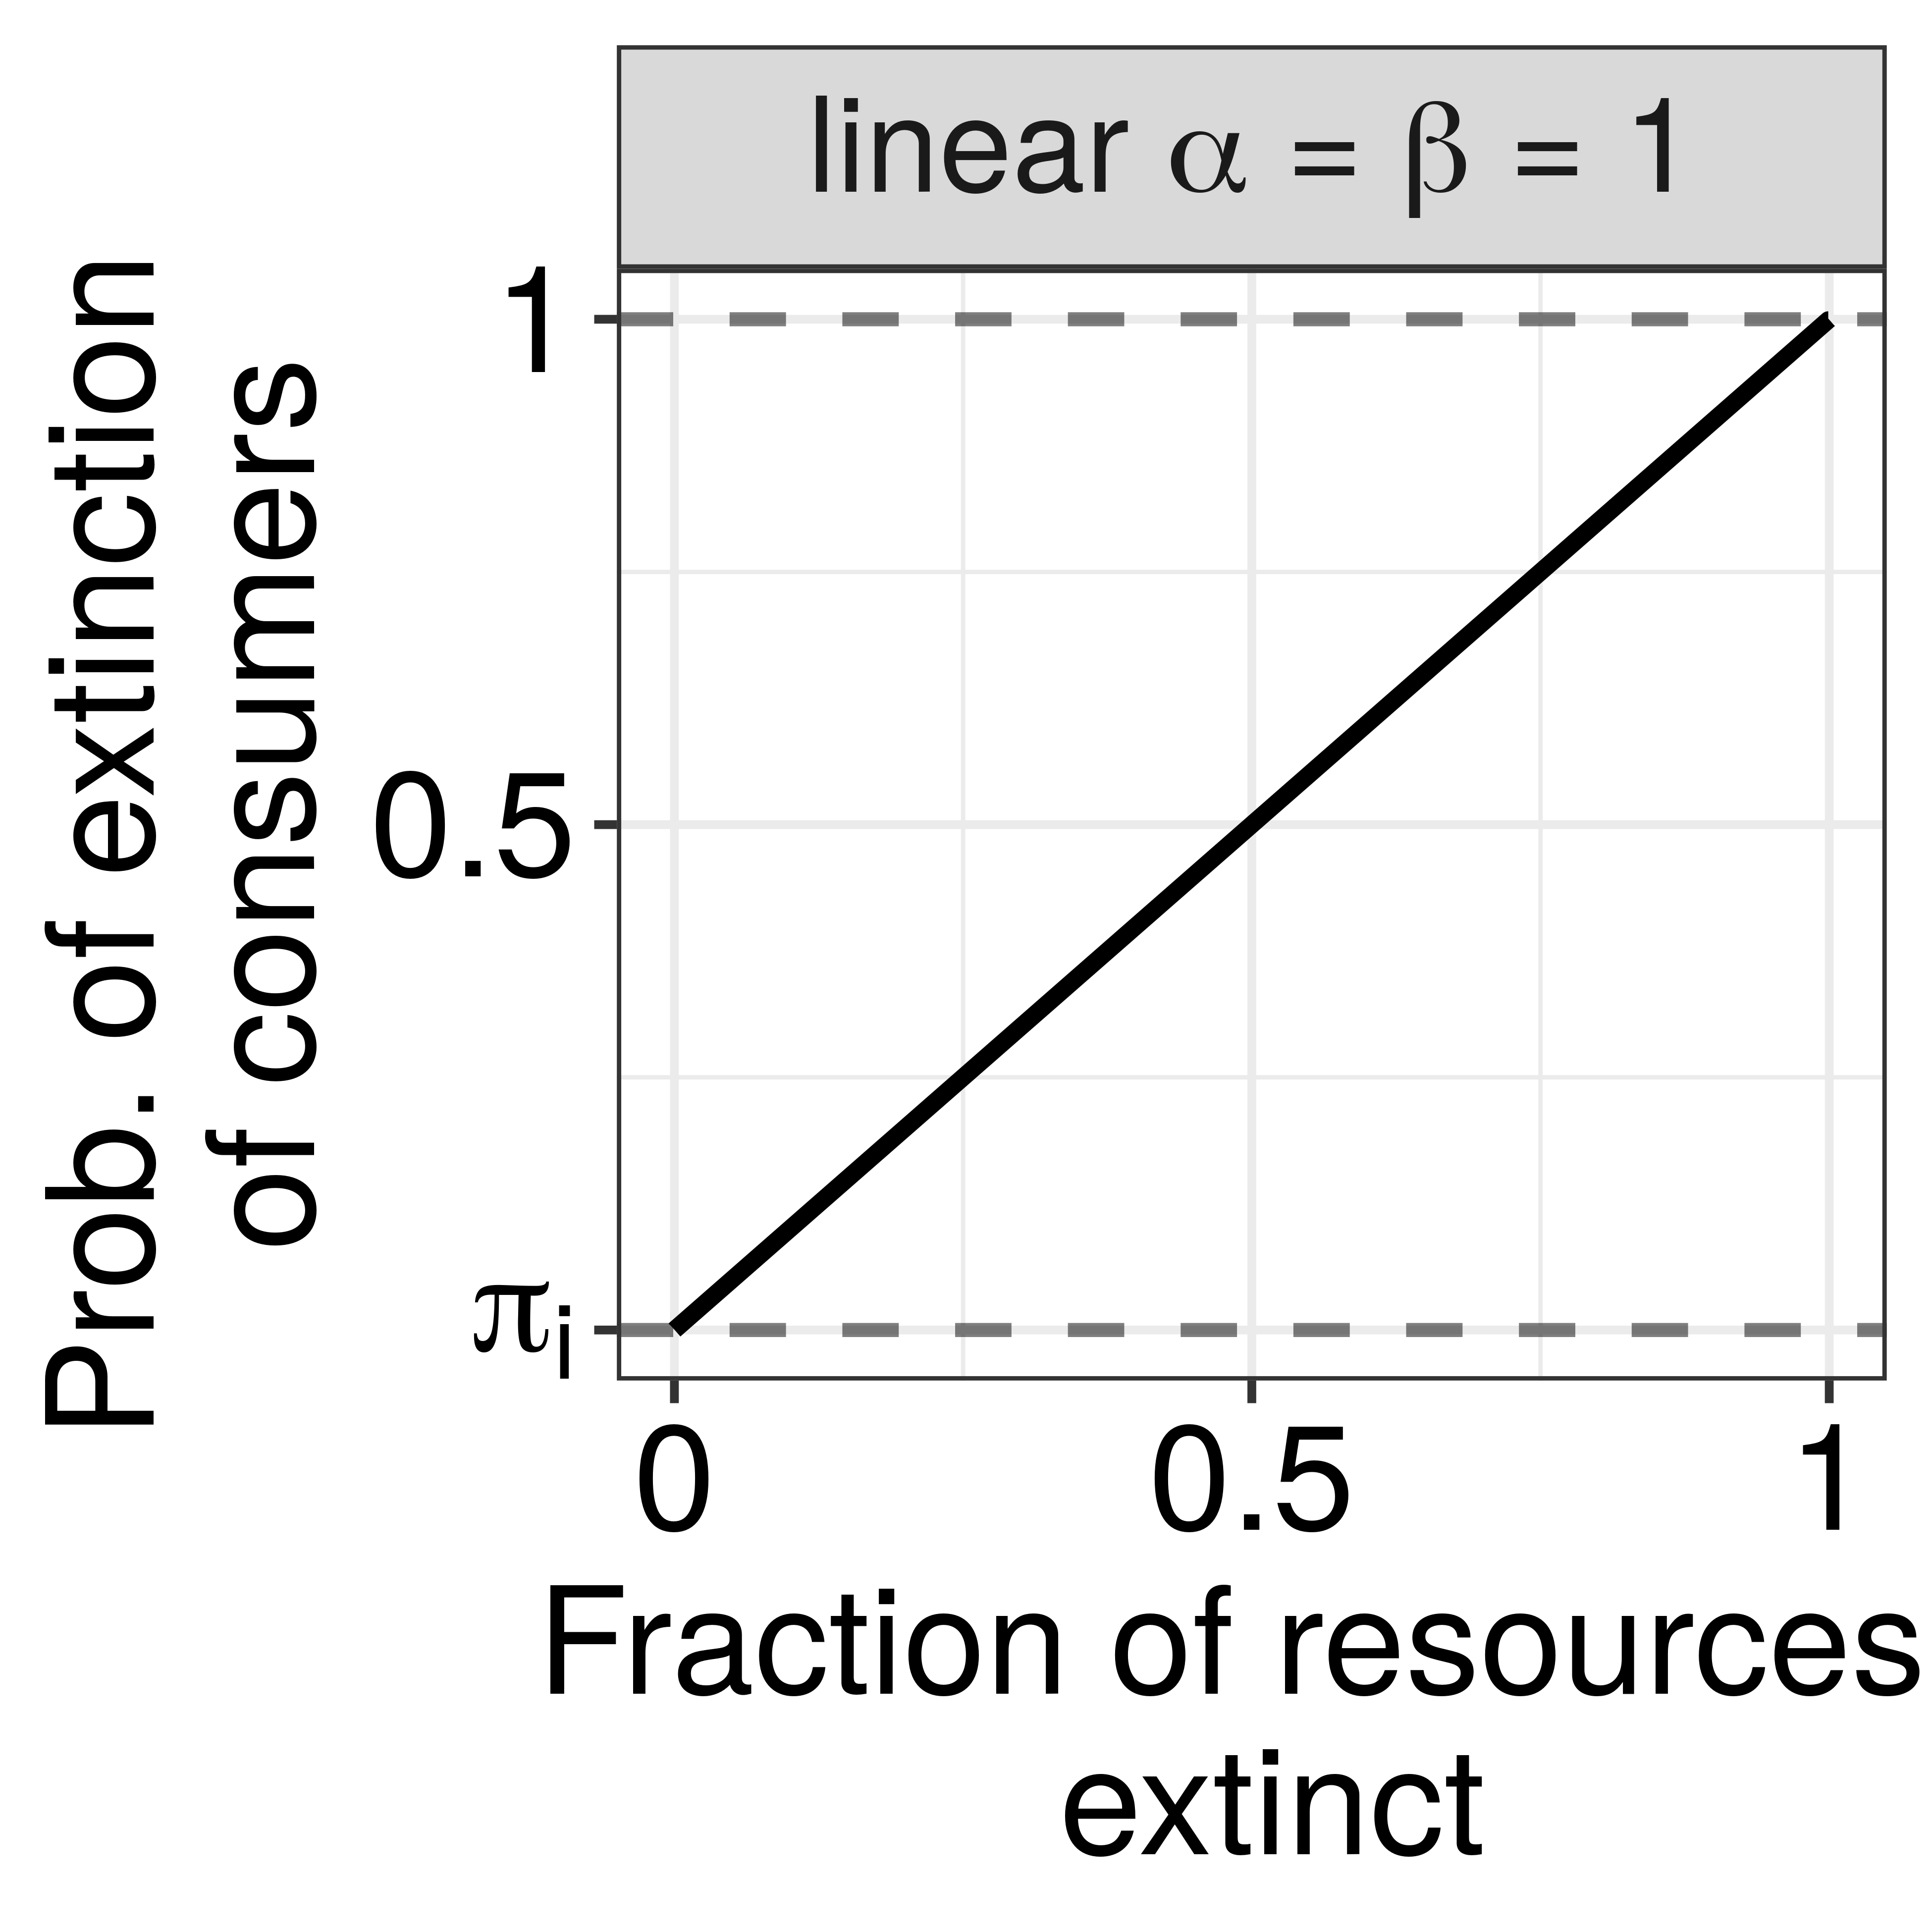
\includegraphics[width=0.19\textwidth,valign=t]{fform_1_1.png}
  \caption{As Figure~\ref{fig:patchloss_web1_11}.}
  \label{fig:patchloss_web3_11}
\end{figure}

\begin{figure}\ContinuedFloat
  \includegraphics[width=0.8\textwidth,valign=t]{lambda_Model_food_web_with_350_consumer_and_50_basal_species_(3)_Weighted_basal_5_1.pdf}
  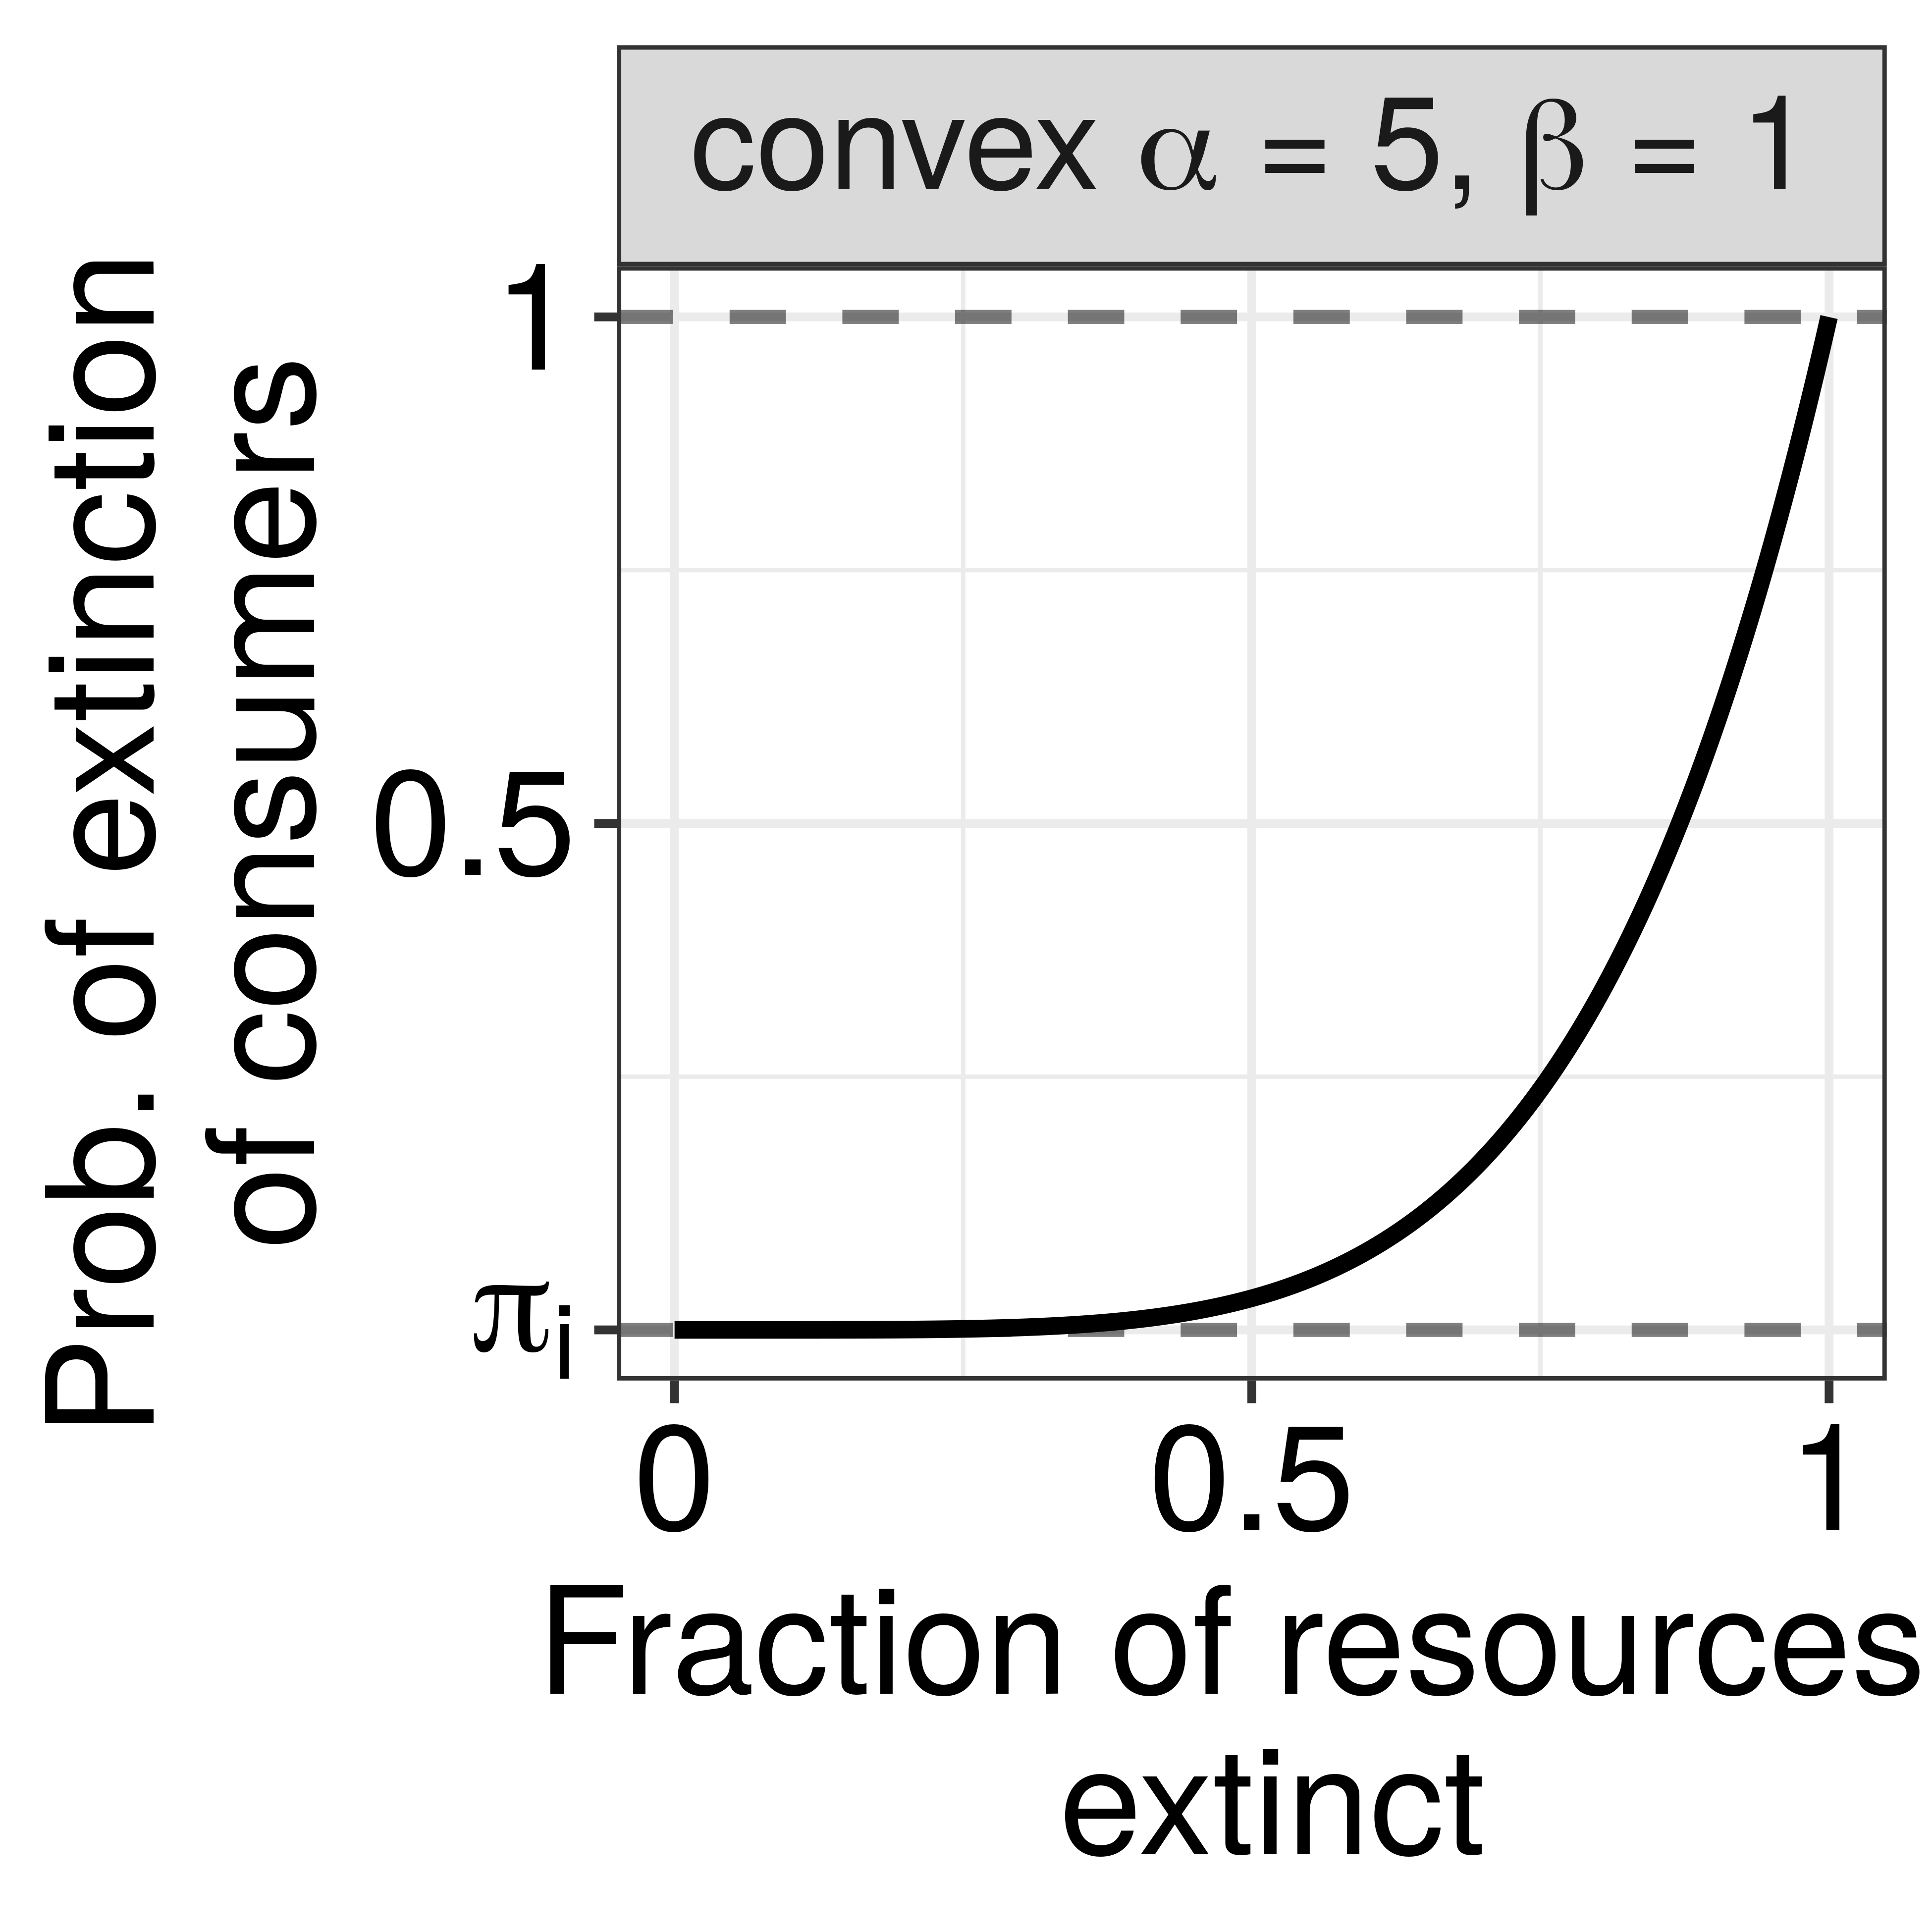
\includegraphics[width=0.19\textwidth,valign=t]{fform_5_1.png}
  \includegraphics[width=0.8\textwidth,valign=t]{lambda_Model_food_web_with_350_consumer_and_50_basal_species_(3)_Not_weighted_basal_5_1.pdf}
  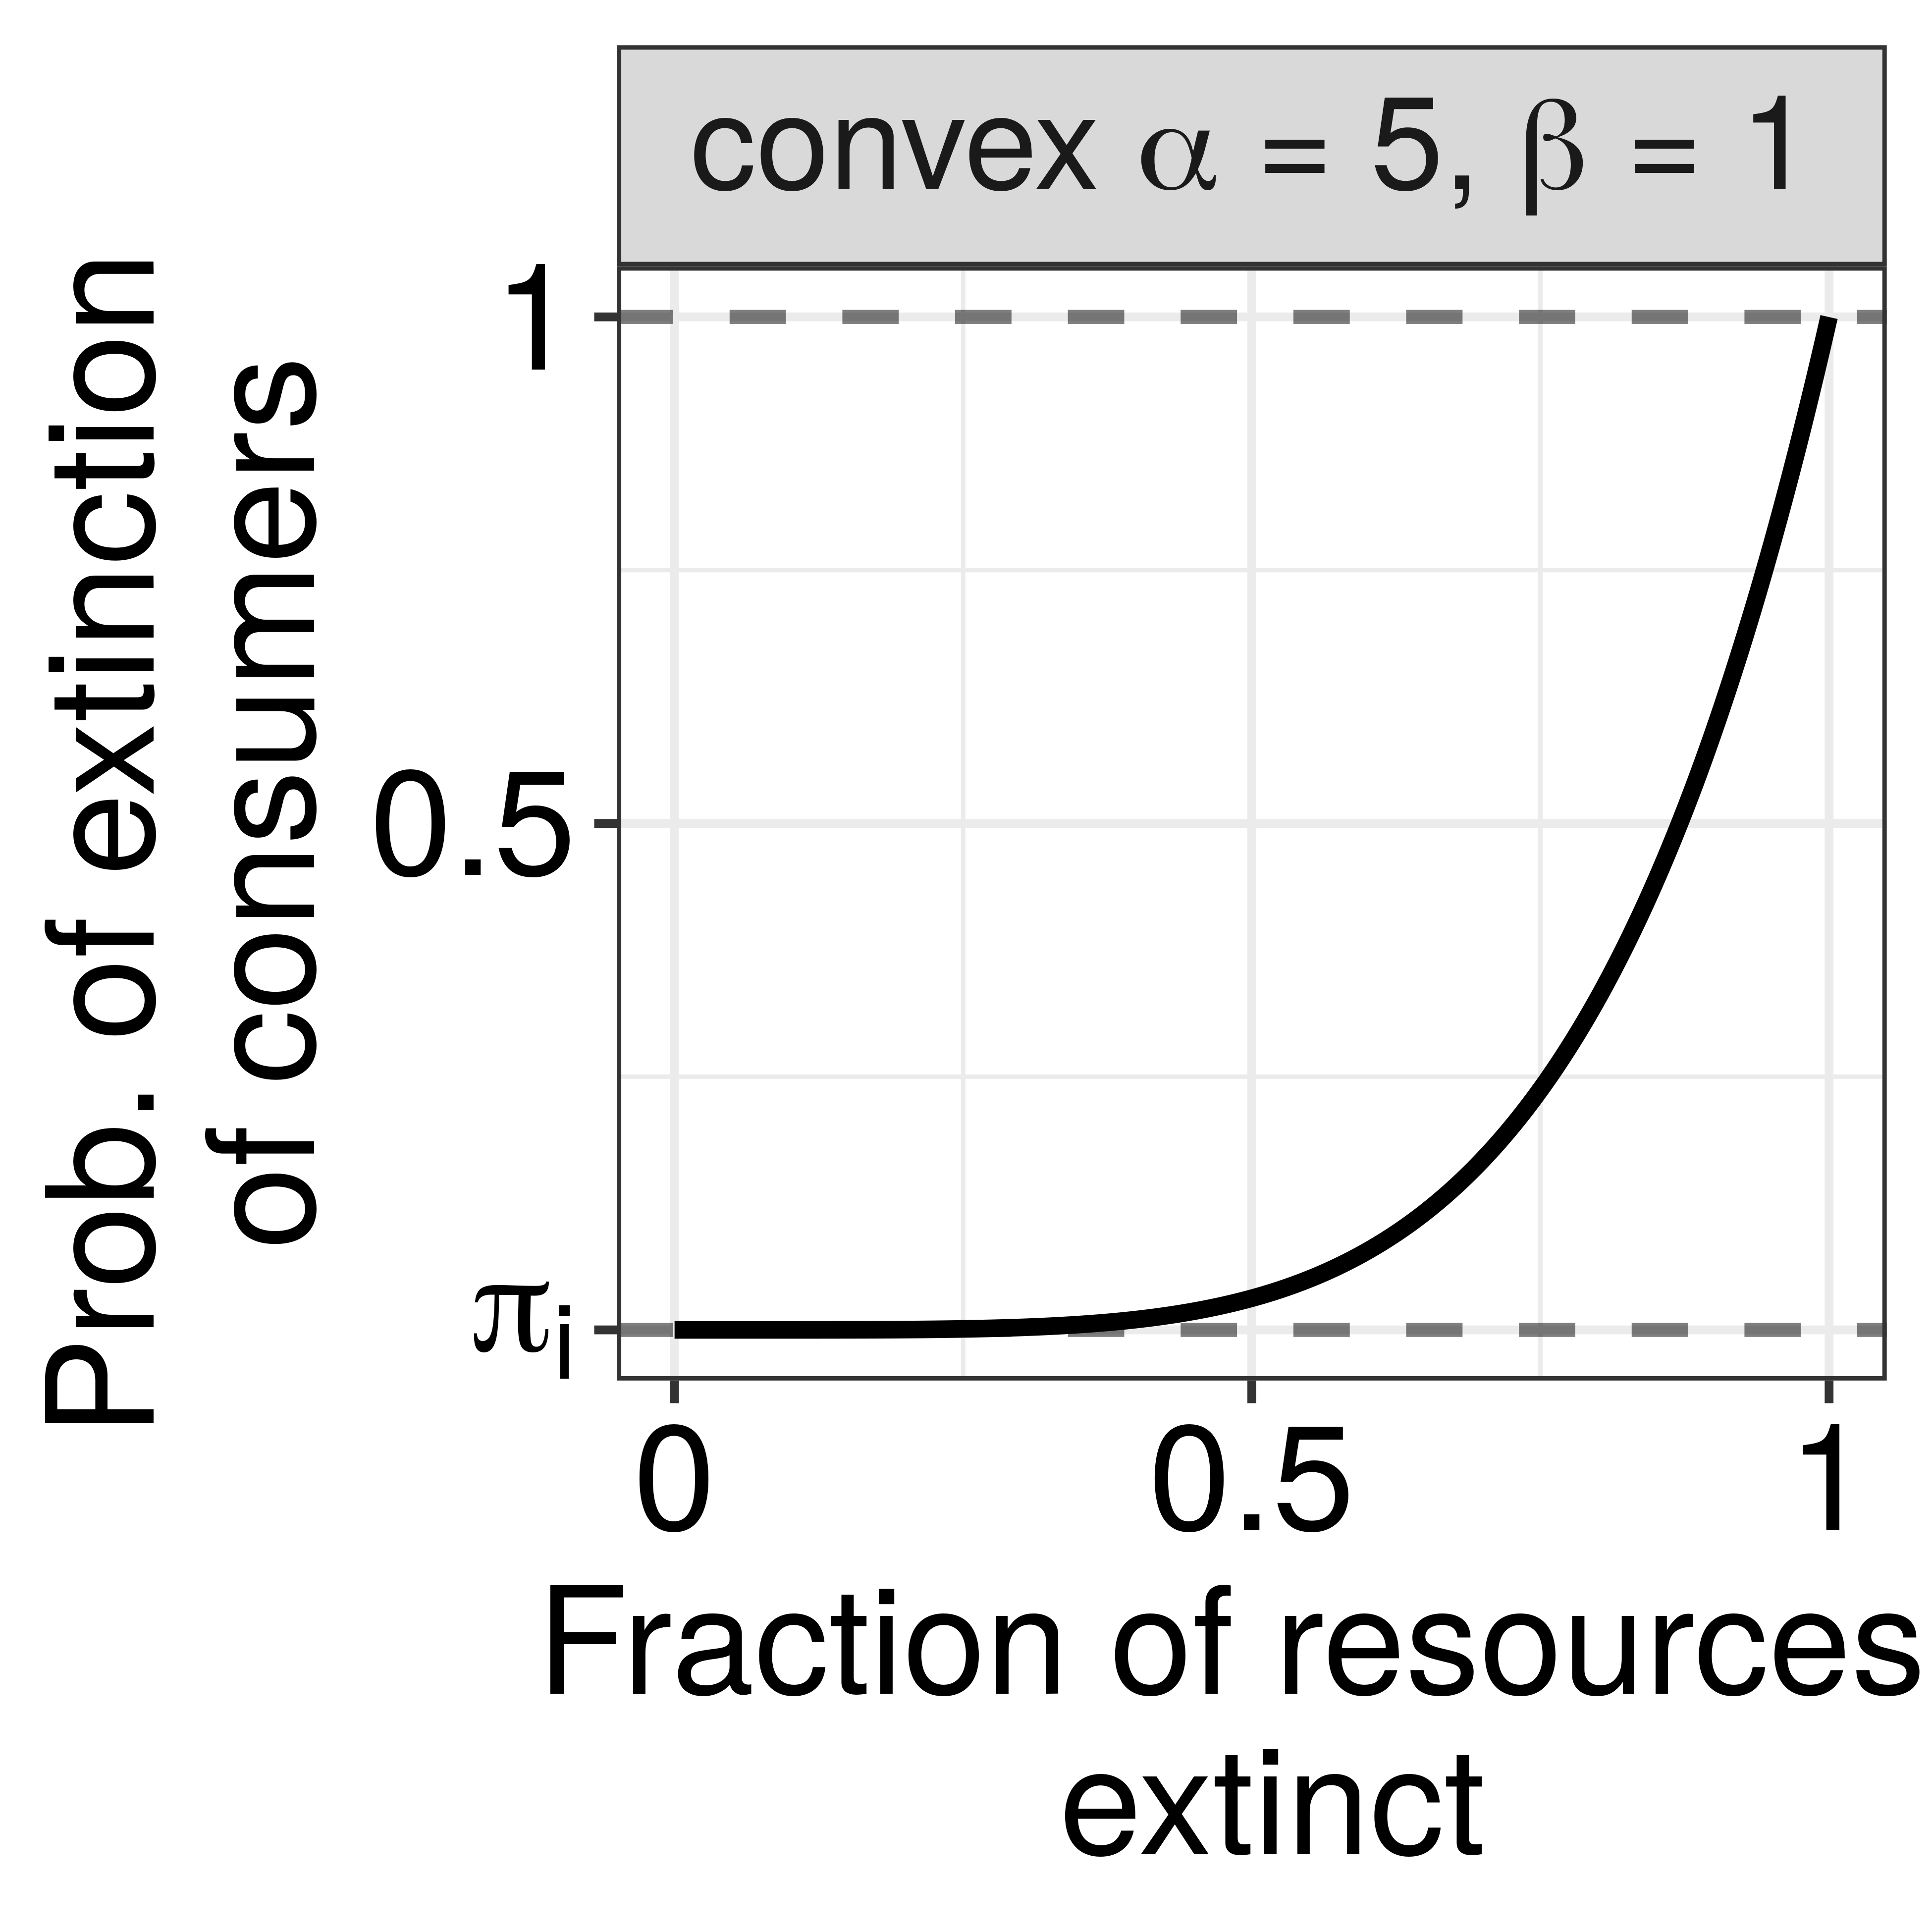
\includegraphics[width=0.19\textwidth,valign=t]{fform_5_1.png}
  \caption{Figure continued.}
  \label{fig:patchloss_web3_51}
\end{figure}

\begin{figure}\ContinuedFloat
  \includegraphics[width=0.8\textwidth,valign=t]{lambda_Model_food_web_with_350_consumer_and_50_basal_species_(3)_Weighted_basal_1_5.pdf}
  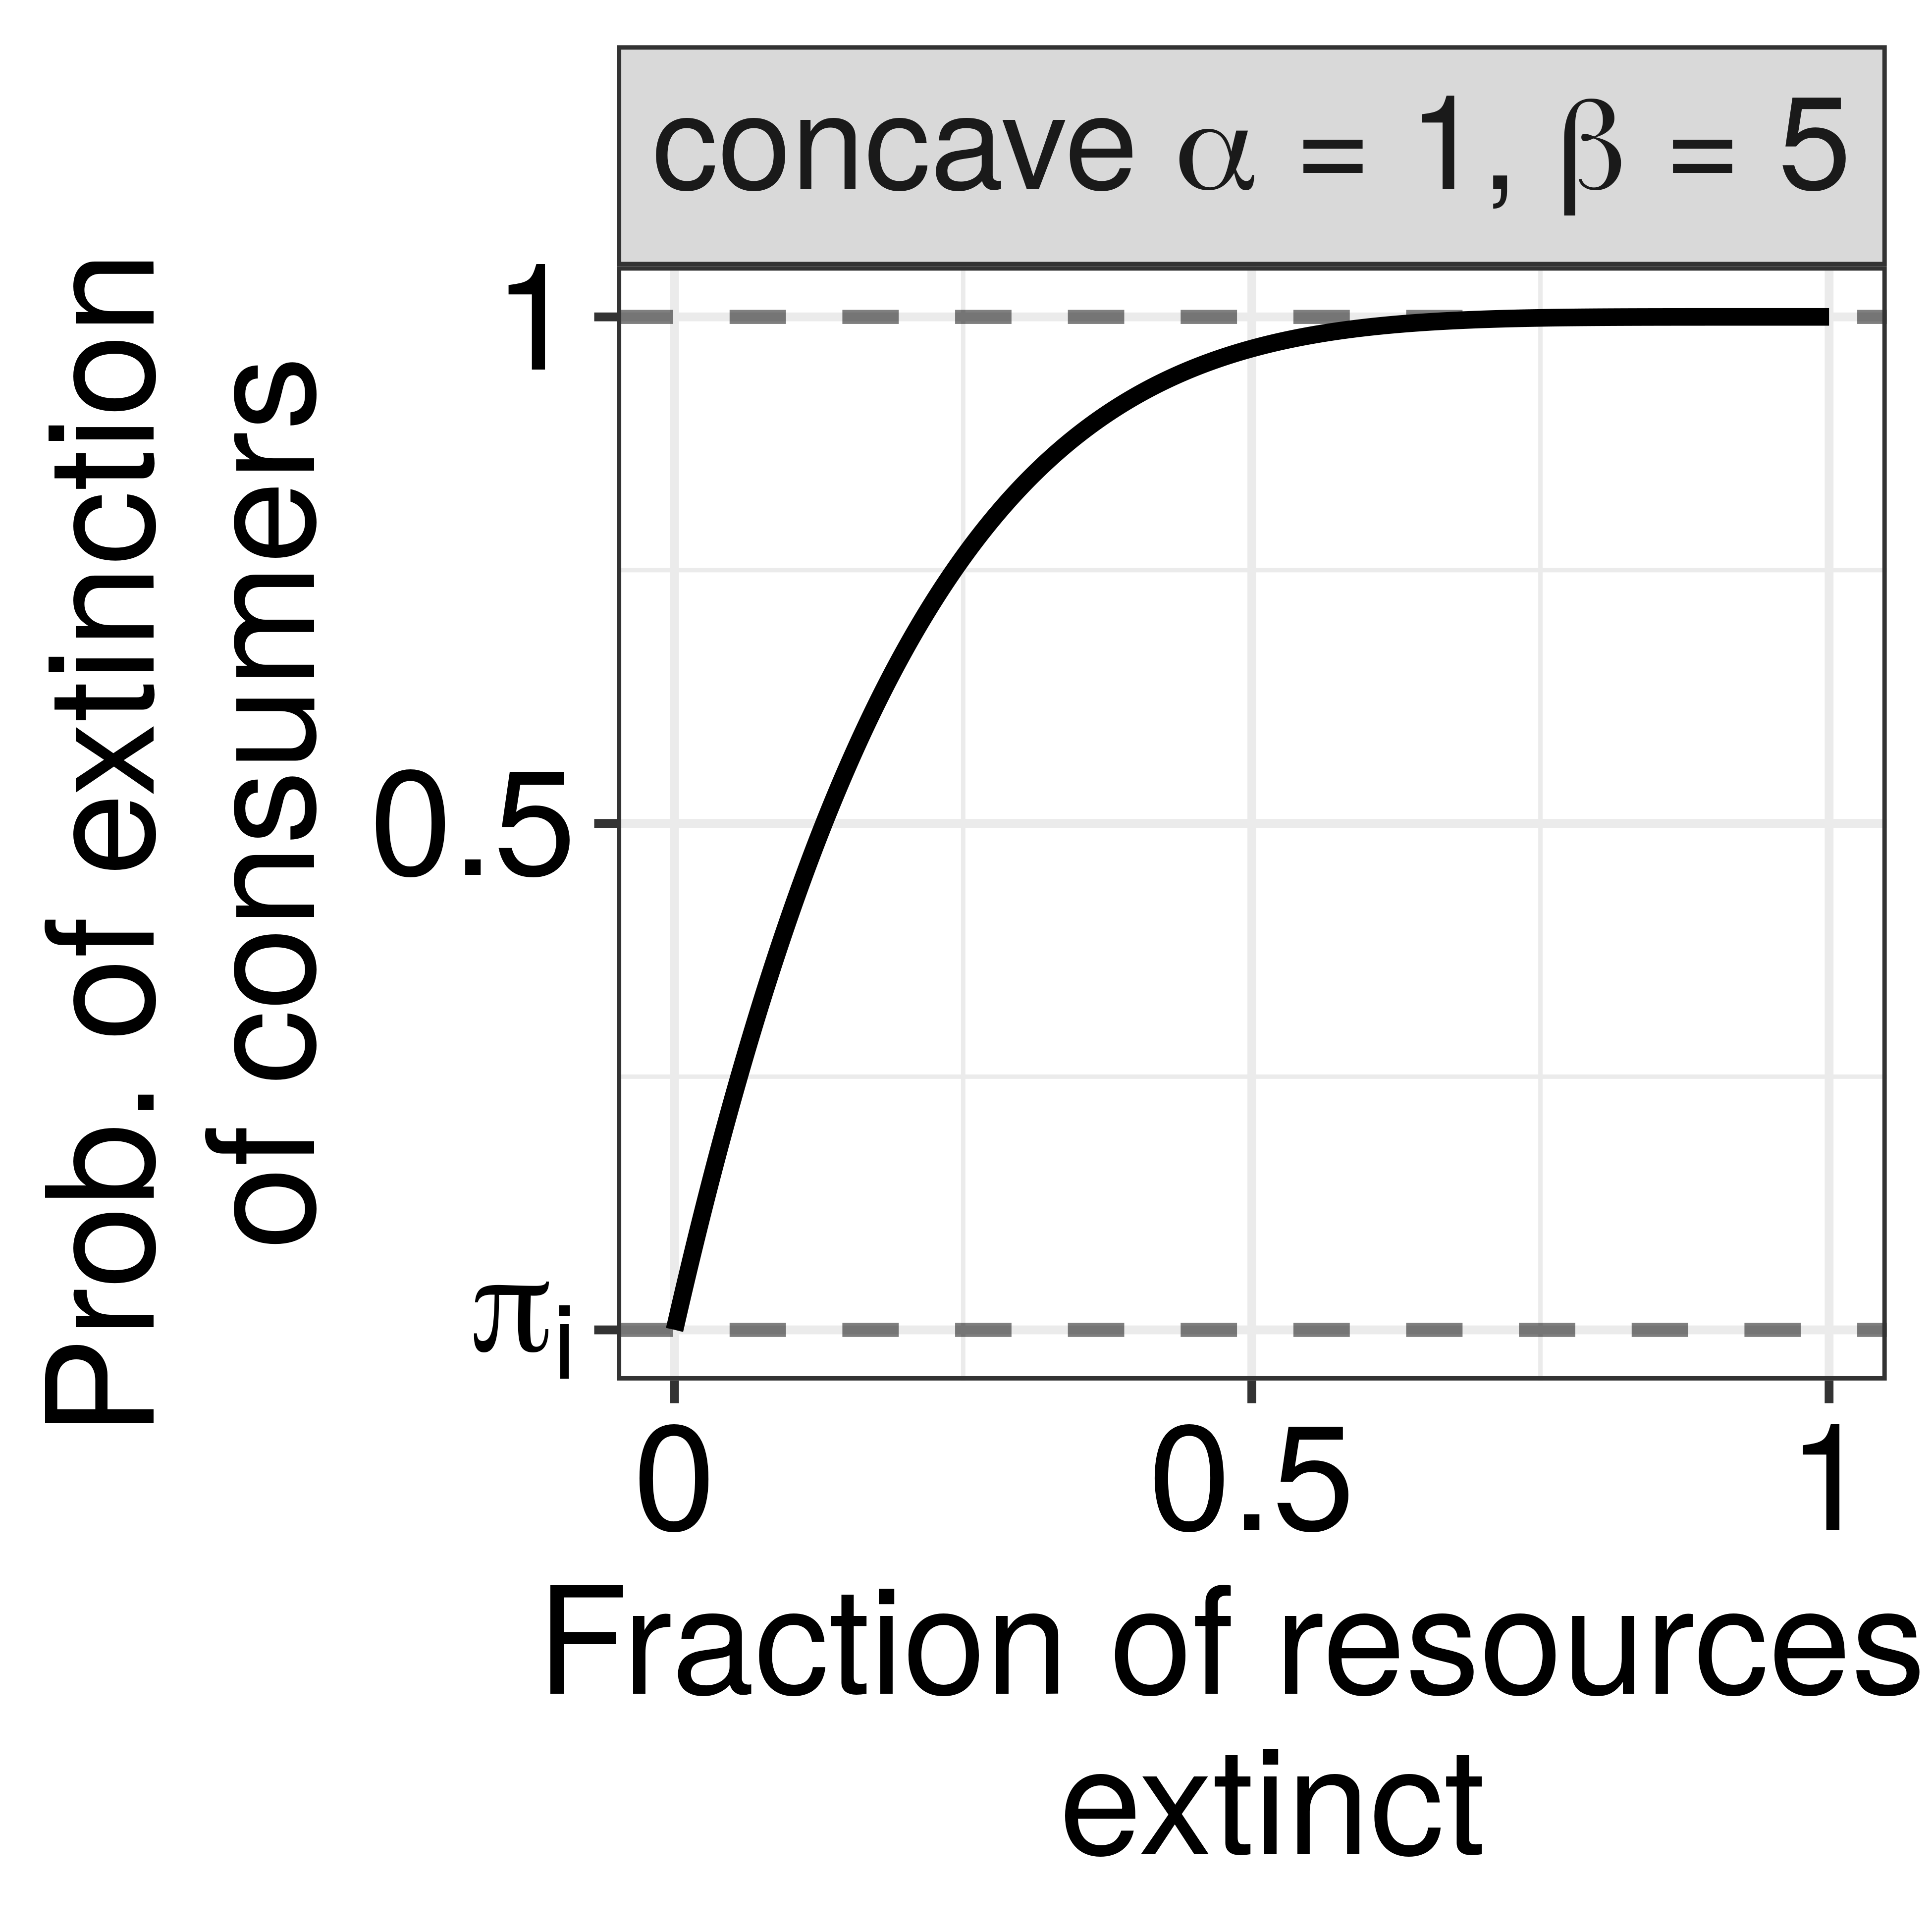
\includegraphics[width=0.19\textwidth,valign=t]{fform_1_5.png}
  \includegraphics[width=0.8\textwidth,valign=t]{lambda_Model_food_web_with_350_consumer_and_50_basal_species_(3)_Not_weighted_basal_1_5.pdf}
  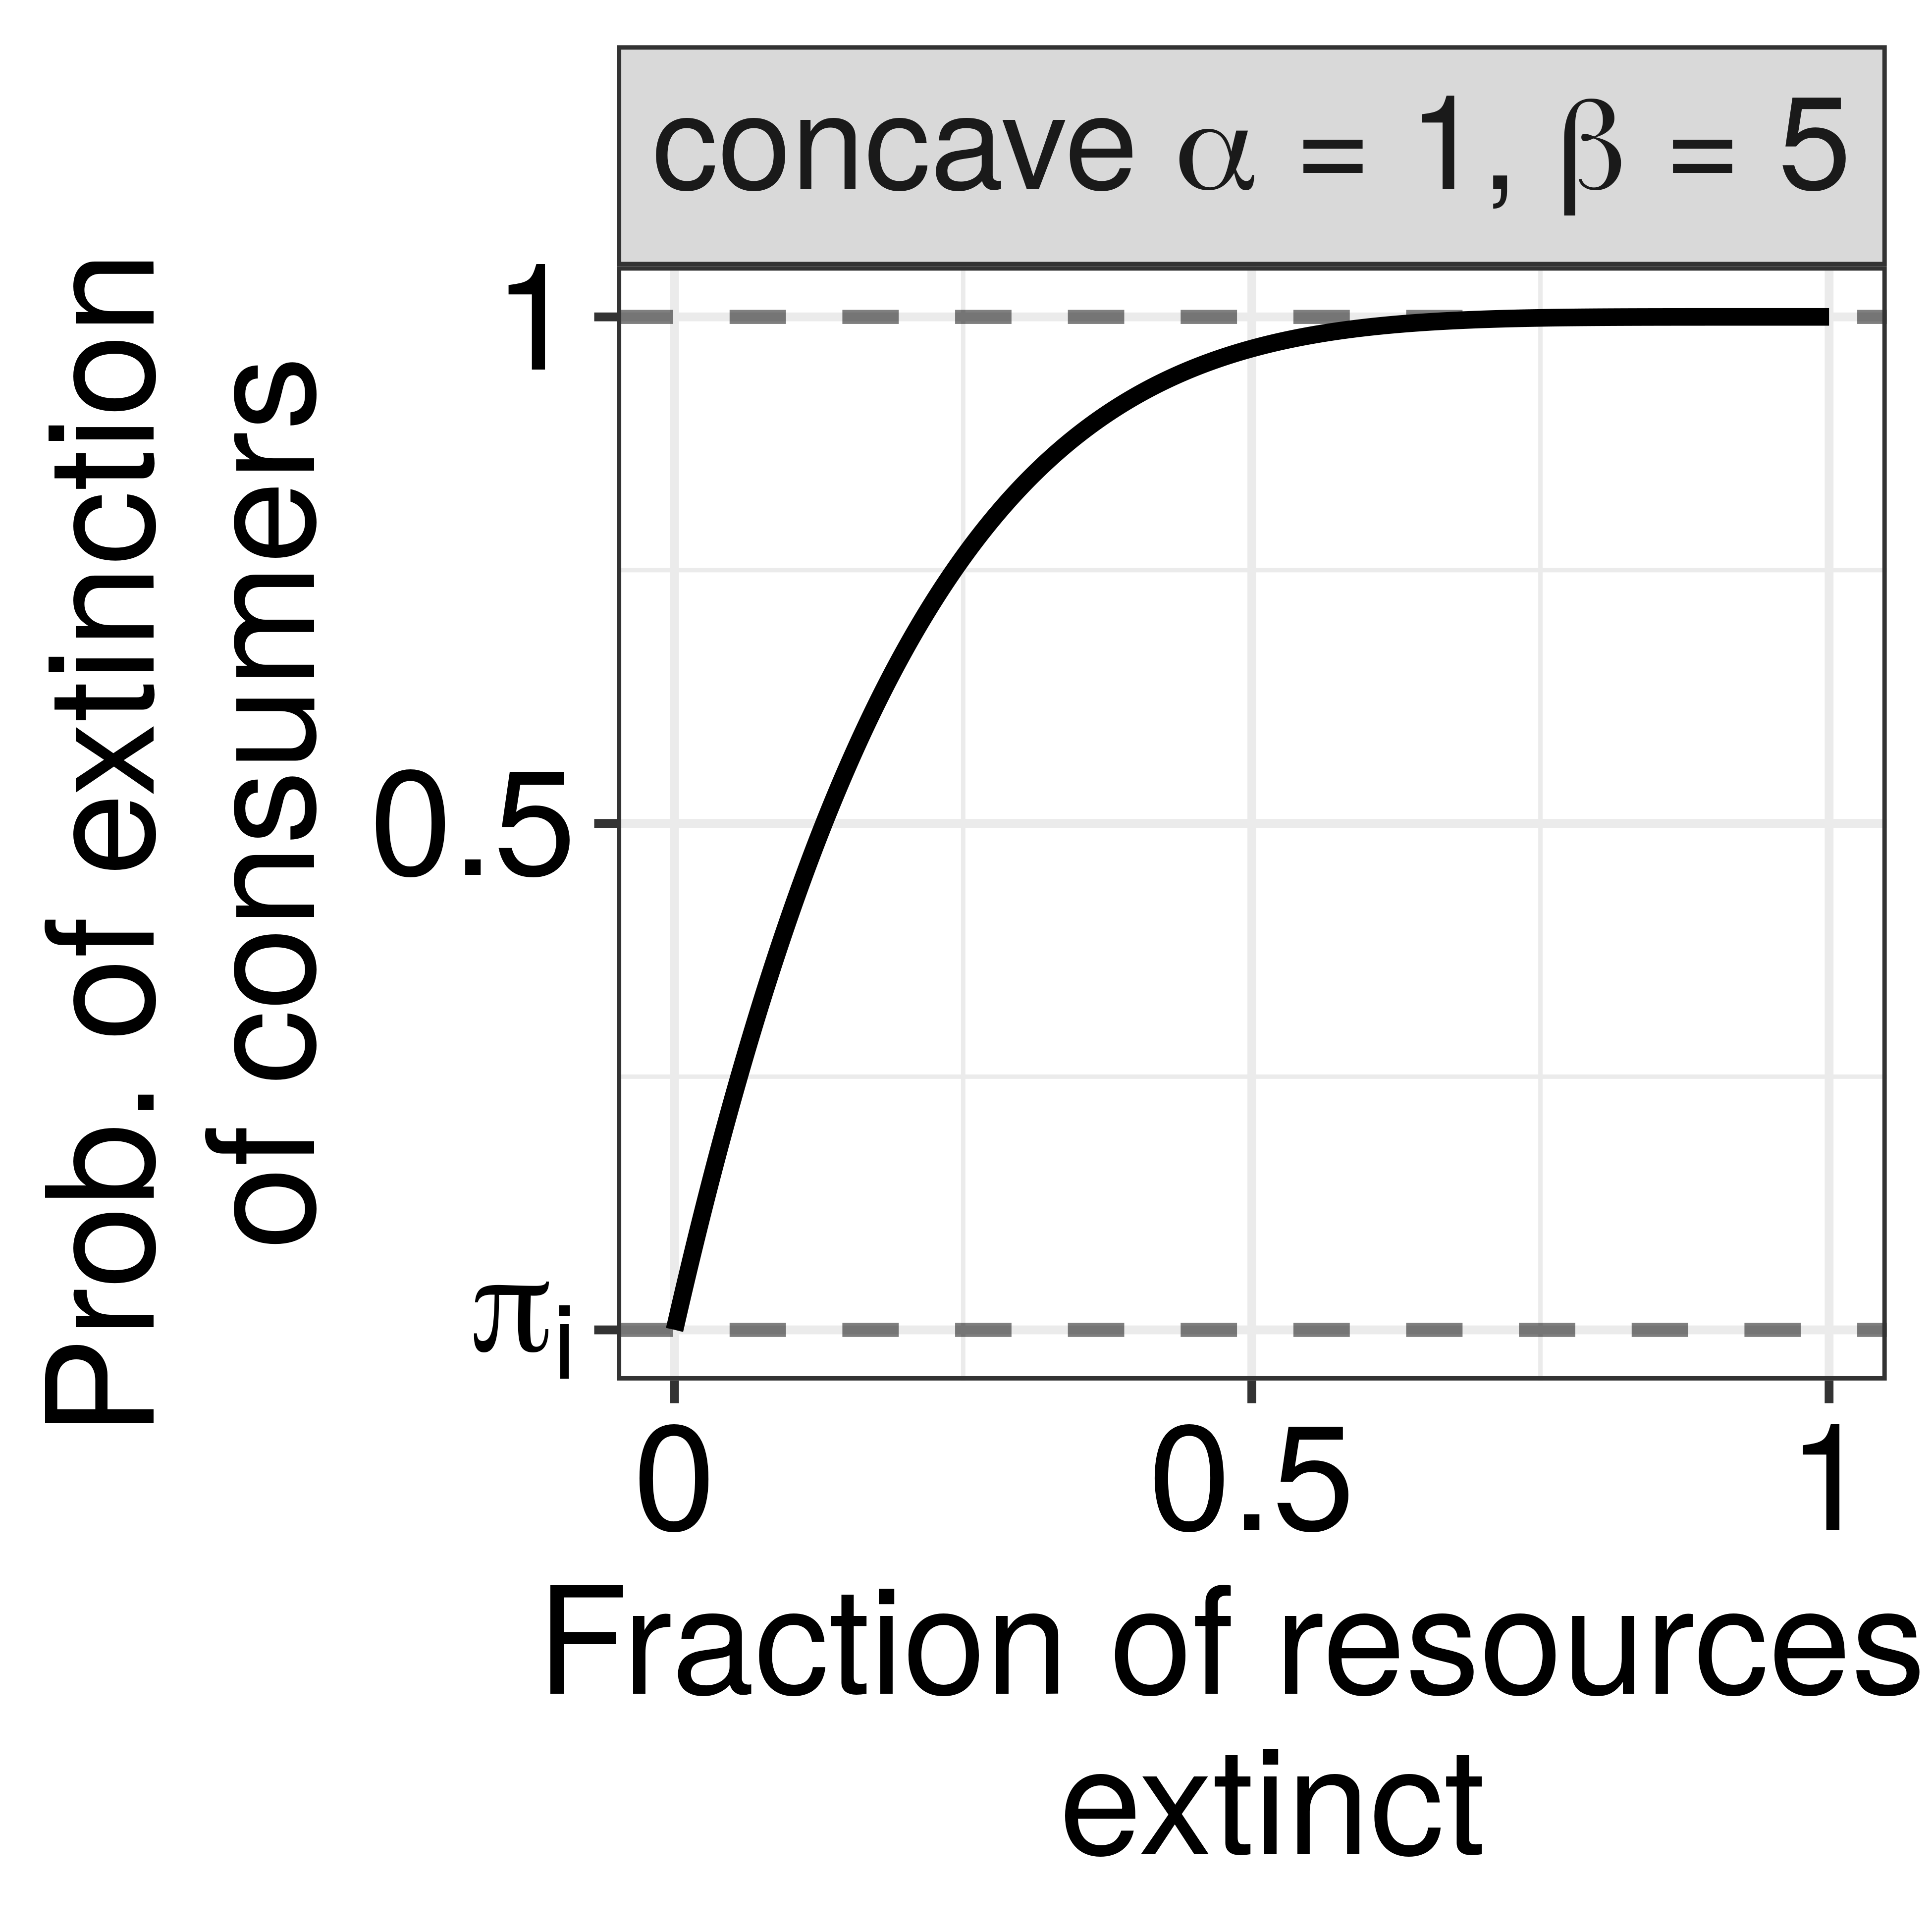
\includegraphics[width=0.19\textwidth,valign=t]{fform_1_5.png}
  \caption{Figure continued.}
  \label{fig:patchloss_web3_15}
\end{figure}

\begin{figure}\ContinuedFloat
  \includegraphics[width=0.8\textwidth,valign=t]{lambda_Model_food_web_with_350_consumer_and_50_basal_species_(3)_Weighted_basal_5_5.pdf}
  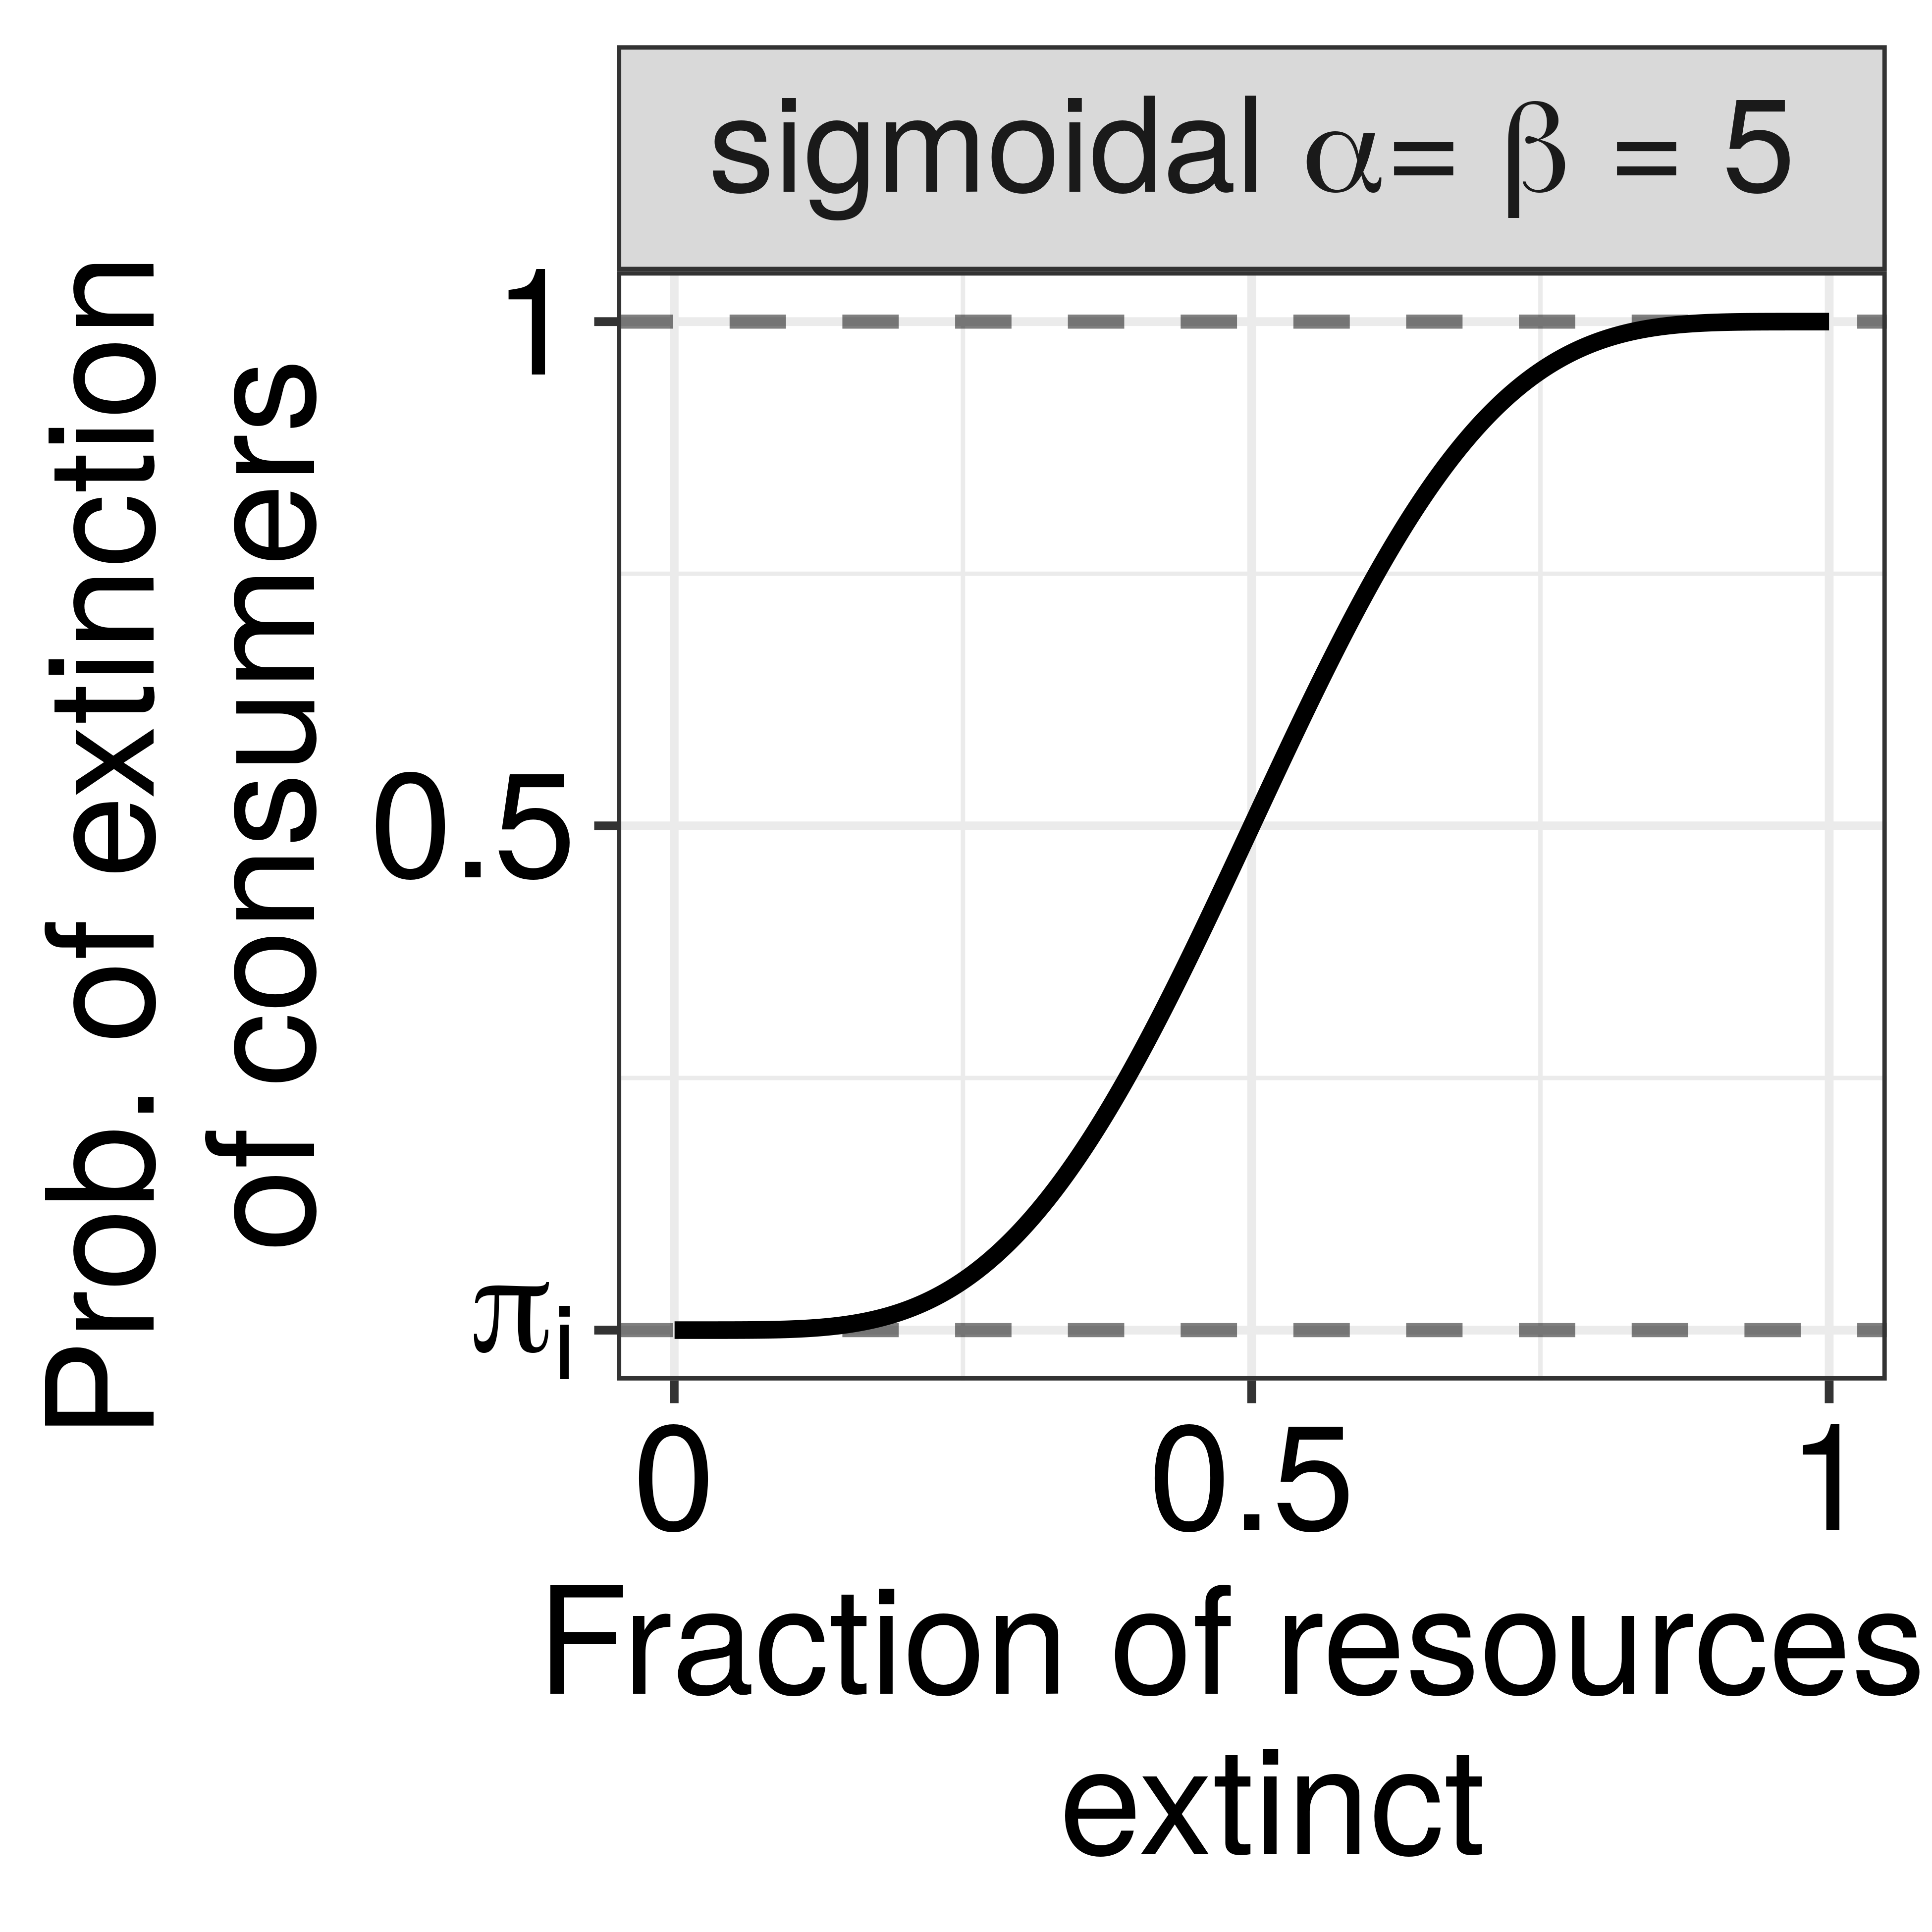
\includegraphics[width=0.19\textwidth,valign=t]{fform_5_5.png}
  \includegraphics[width=0.8\textwidth,valign=t]{lambda_Model_food_web_with_350_consumer_and_50_basal_species_(3)_Not_weighted_basal_5_5.pdf}
  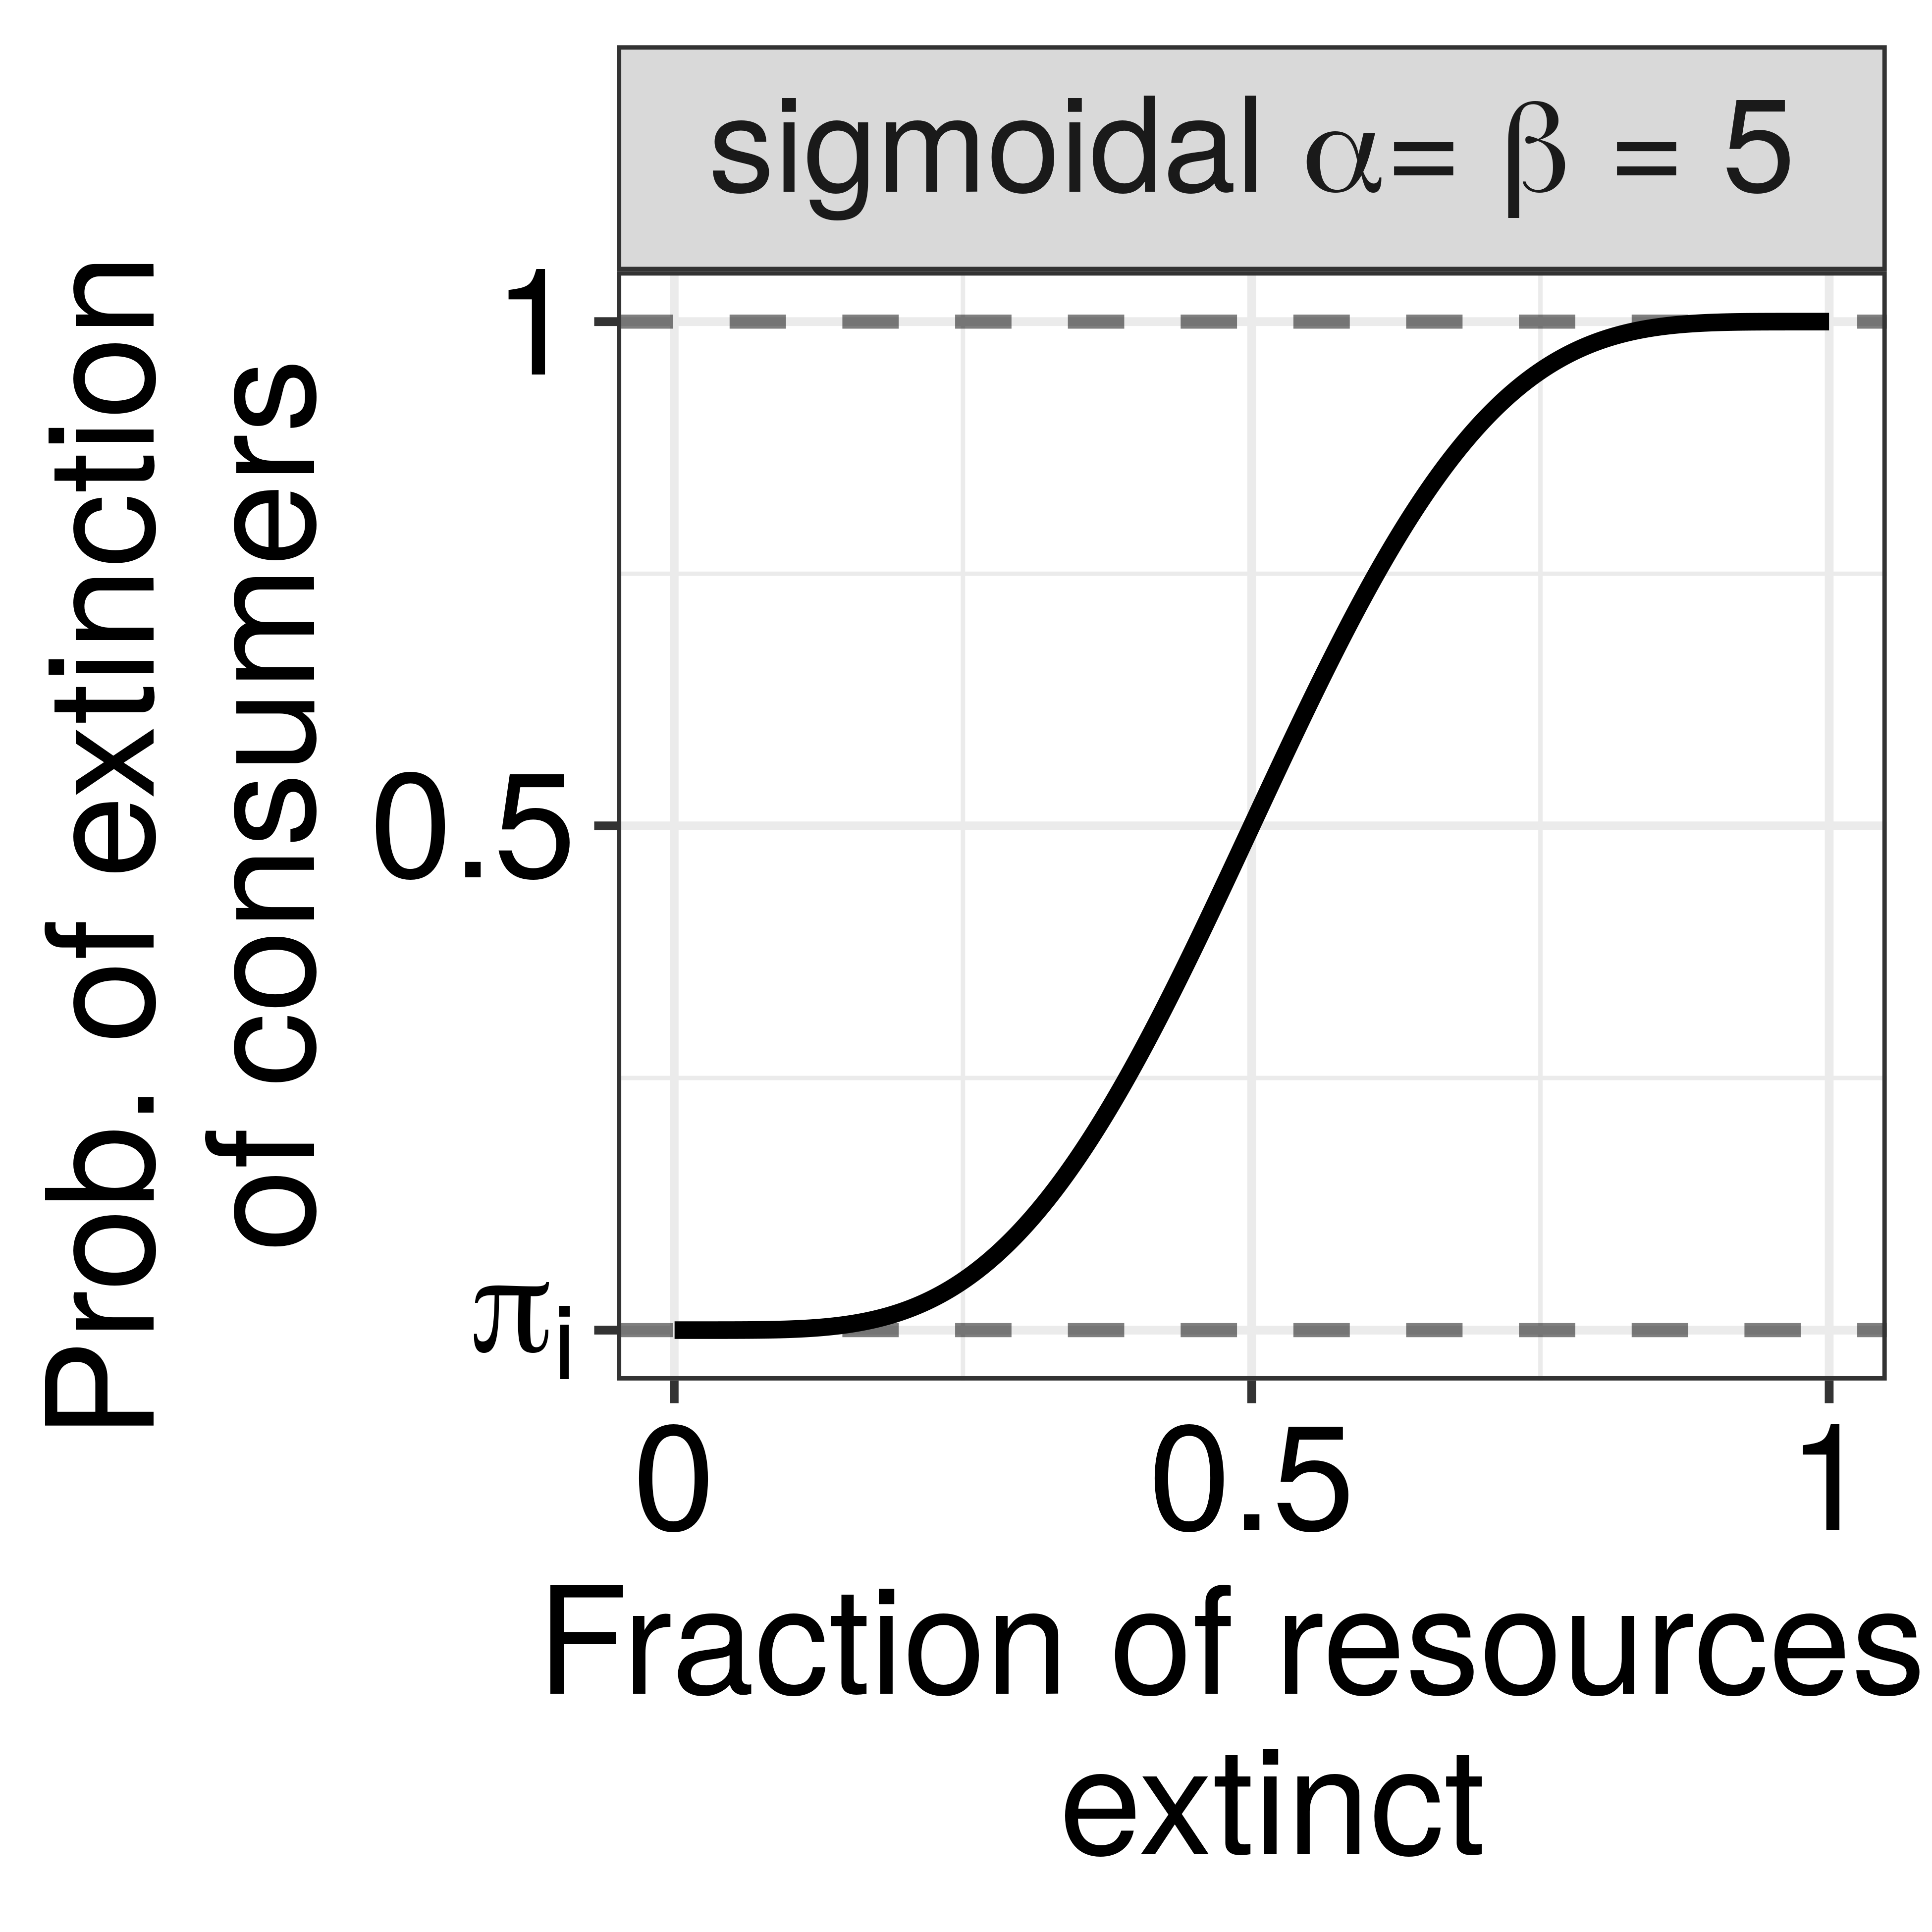
\includegraphics[width=0.19\textwidth,valign=t]{fform_5_5.png}
  \caption{Figure continued.}
  \label{fig:patchloss_web3_55}
\end{figure}

\begin{figure}
  \includegraphics[width=0.8\textwidth,valign=t]{lambda_Model_food_web_with_350_consumer_and_50_basal_species_(4)_Weighted_basal_1_1.pdf}
  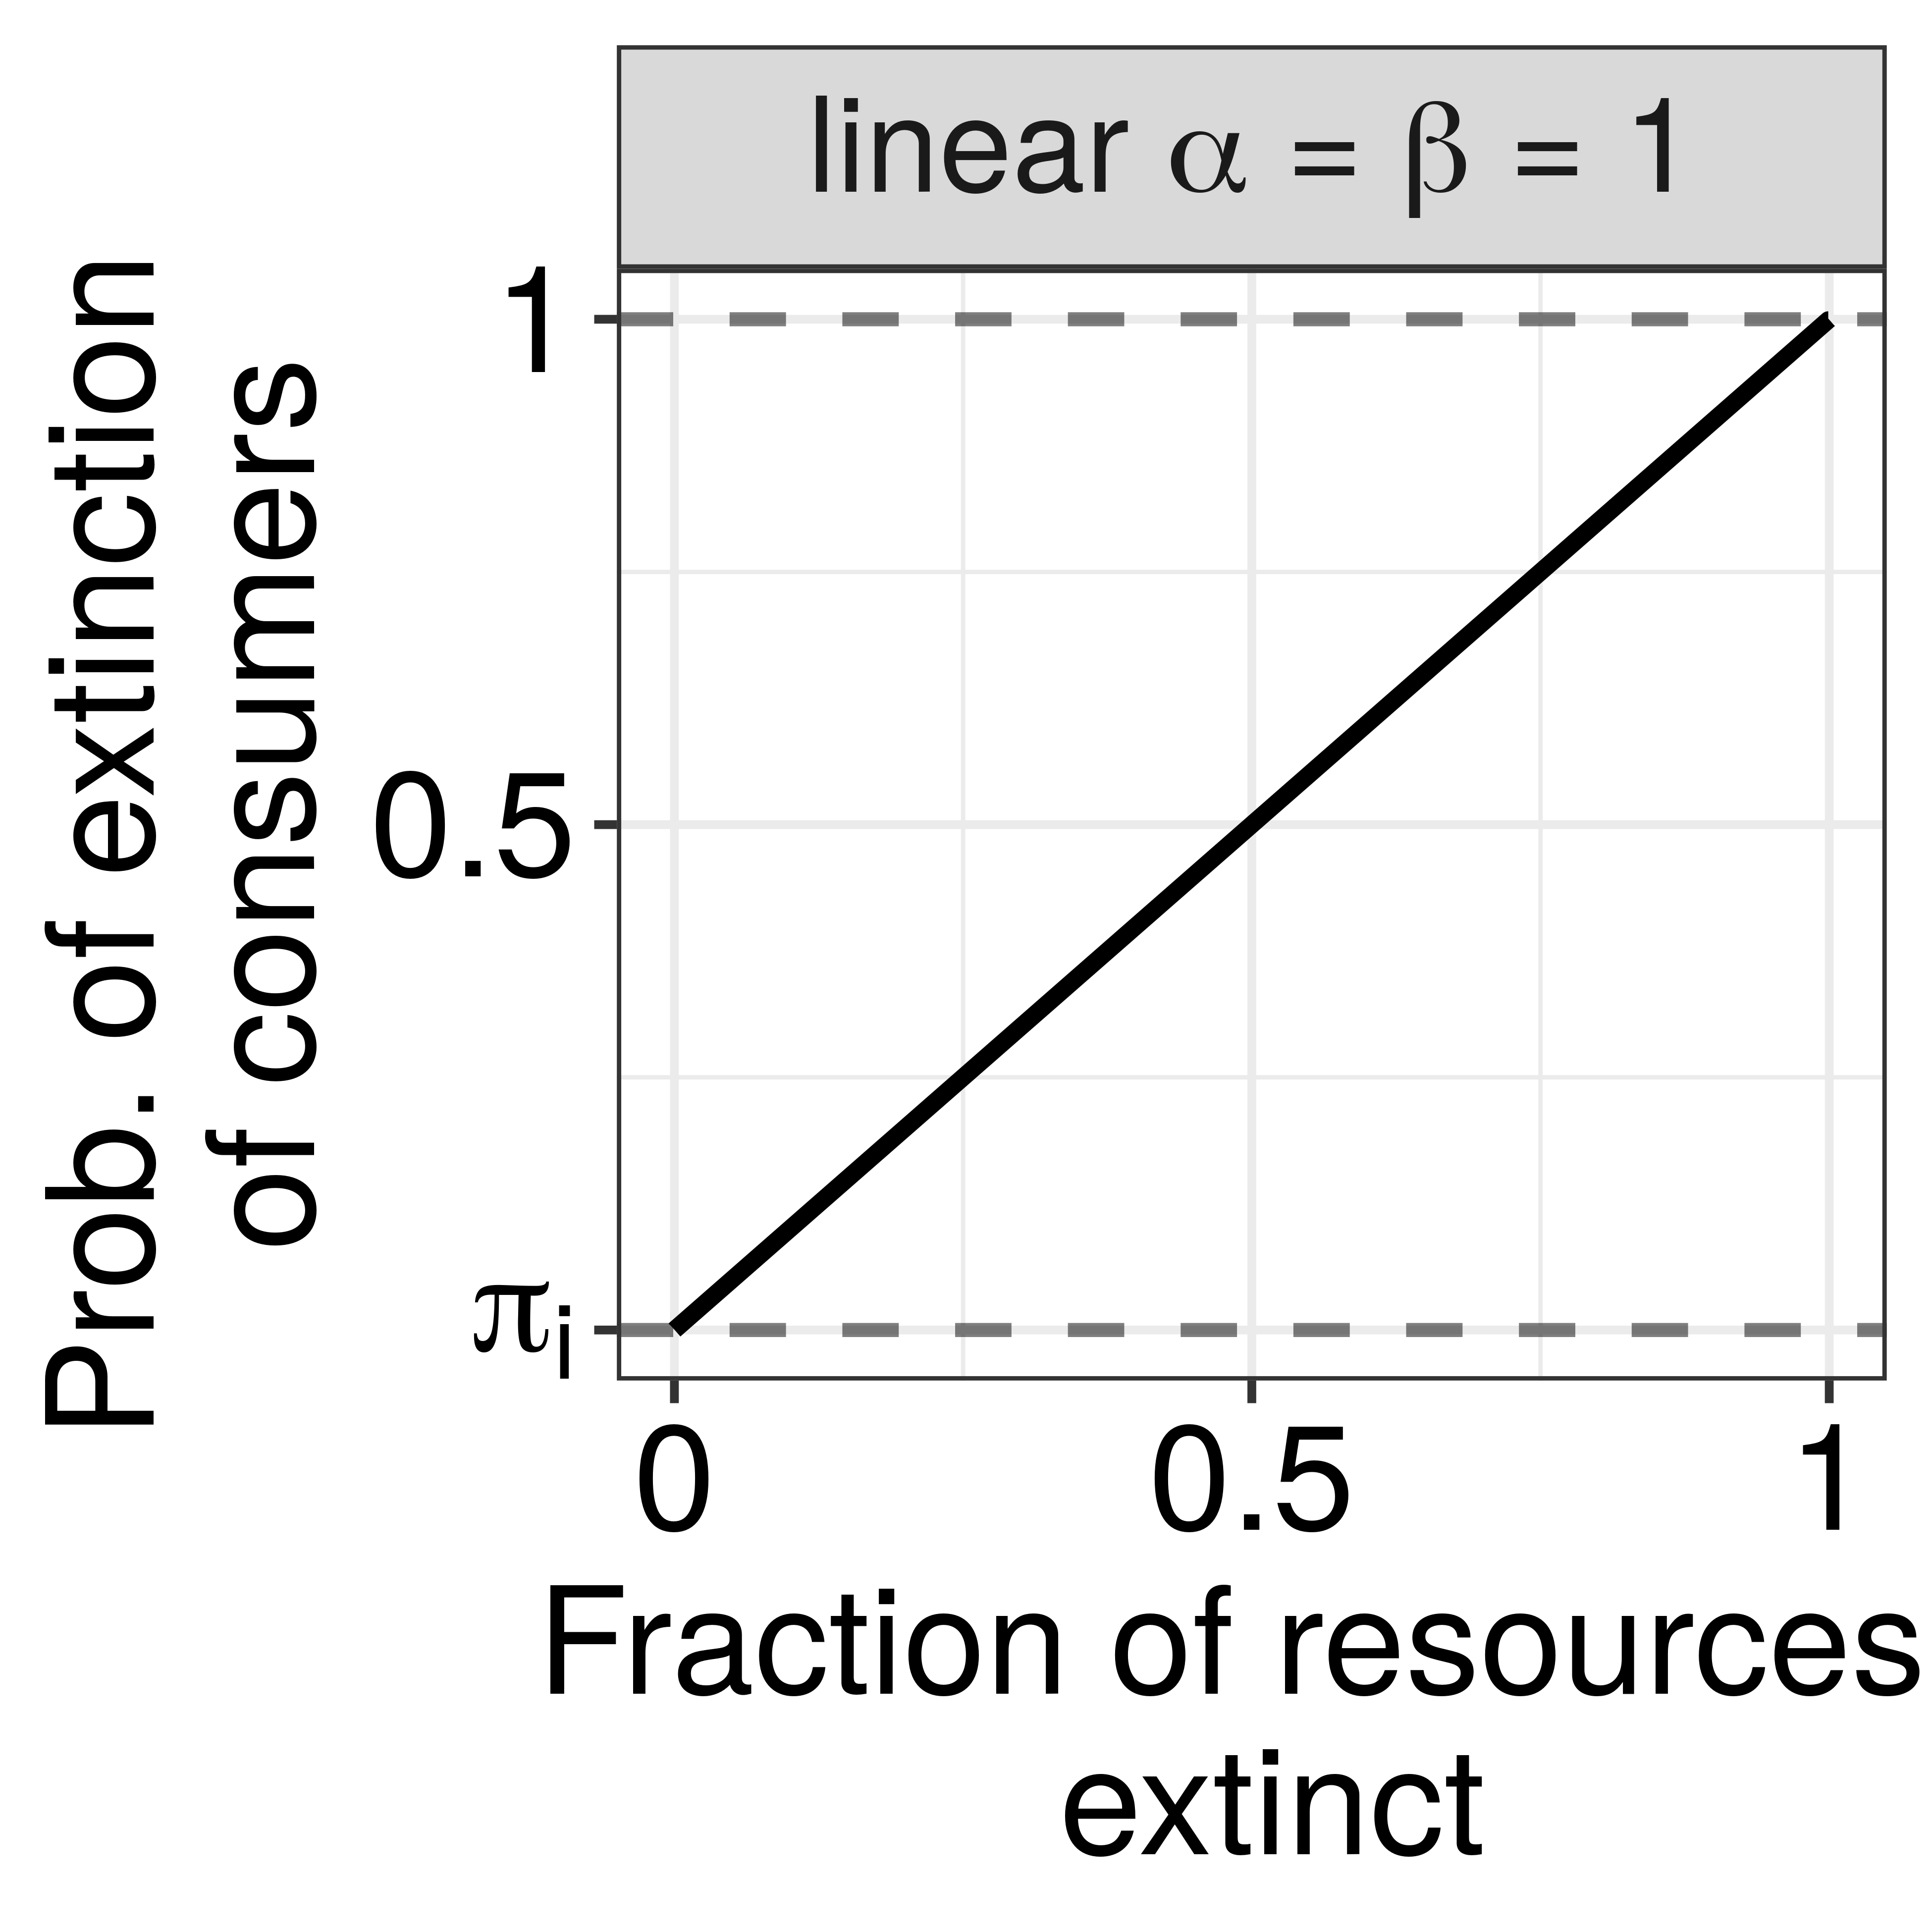
\includegraphics[width=0.19\textwidth,valign=t]{fform_1_1.png}
  \includegraphics[width=0.8\textwidth,valign=t]{lambda_Model_food_web_with_350_consumer_and_50_basal_species_(4)_Not_weighted_basal_1_1.pdf}
  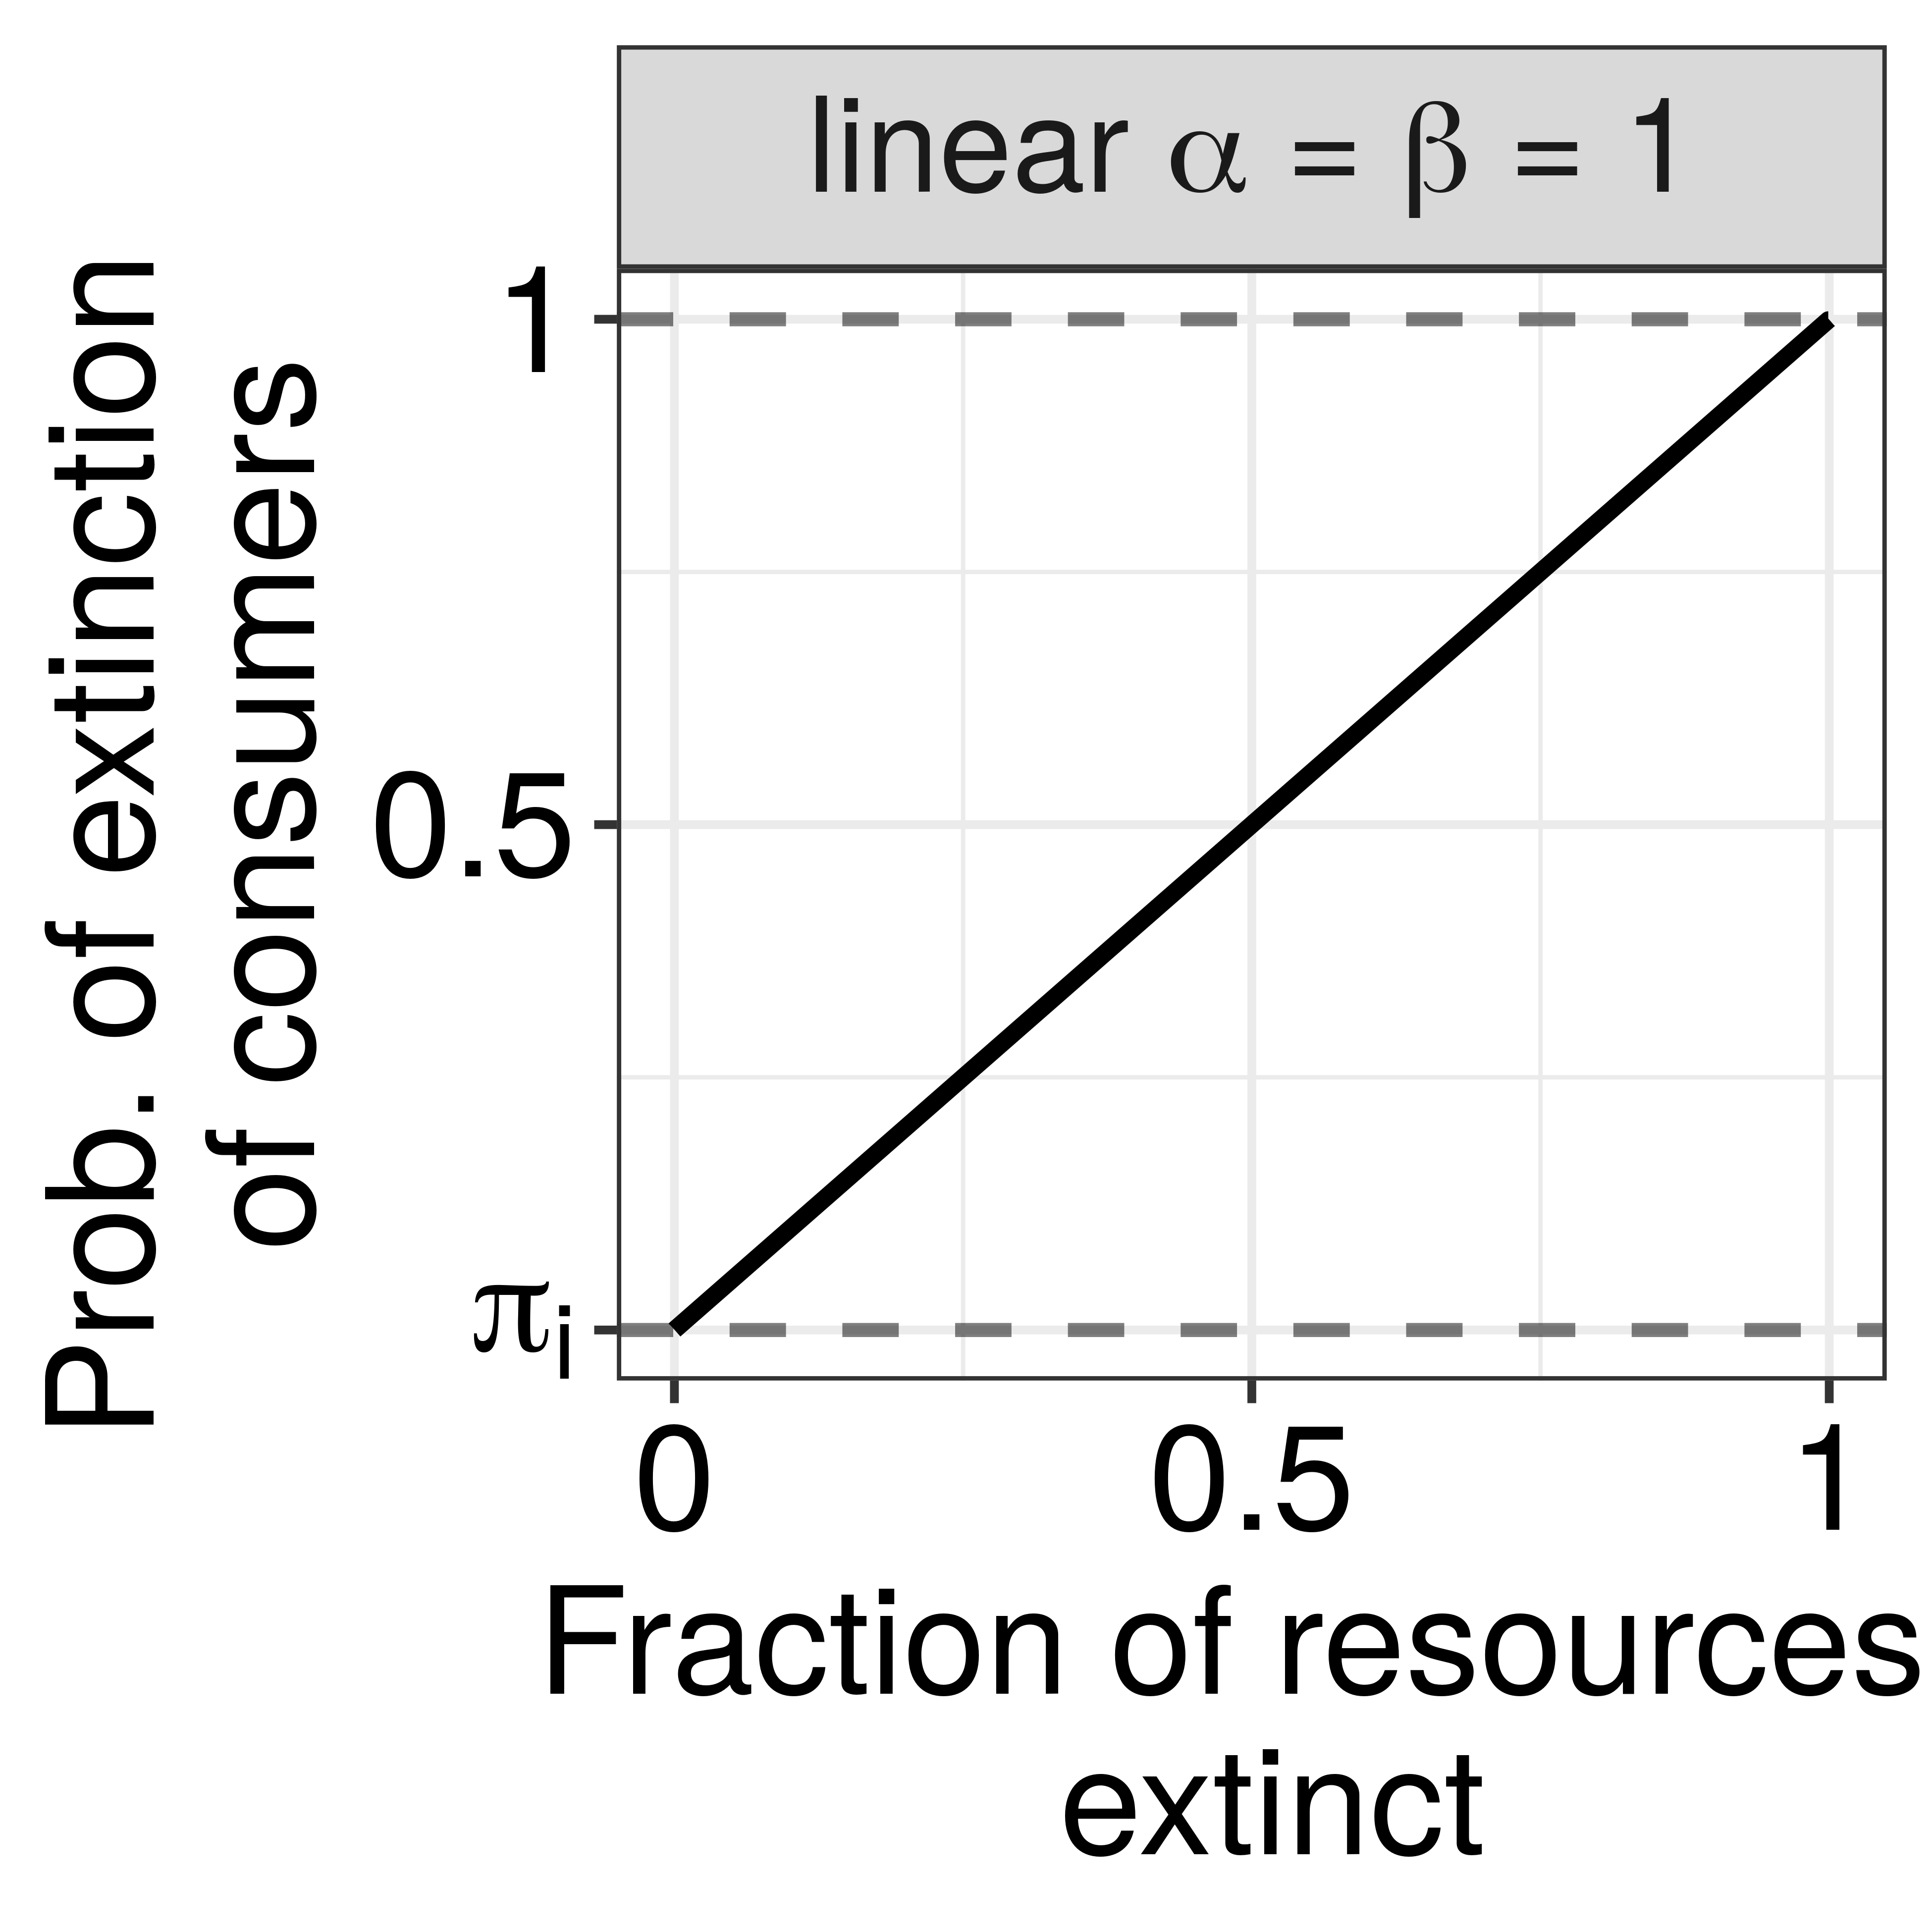
\includegraphics[width=0.19\textwidth,valign=t]{fform_1_1.png}
  \caption{As Figure~\ref{fig:patchloss_web1_11}.}
  \label{fig:patchloss_web4_11}
\end{figure}

\begin{figure}\ContinuedFloat
  \includegraphics[width=0.8\textwidth,valign=t]{lambda_Model_food_web_with_350_consumer_and_50_basal_species_(4)_Weighted_basal_5_1.pdf}
  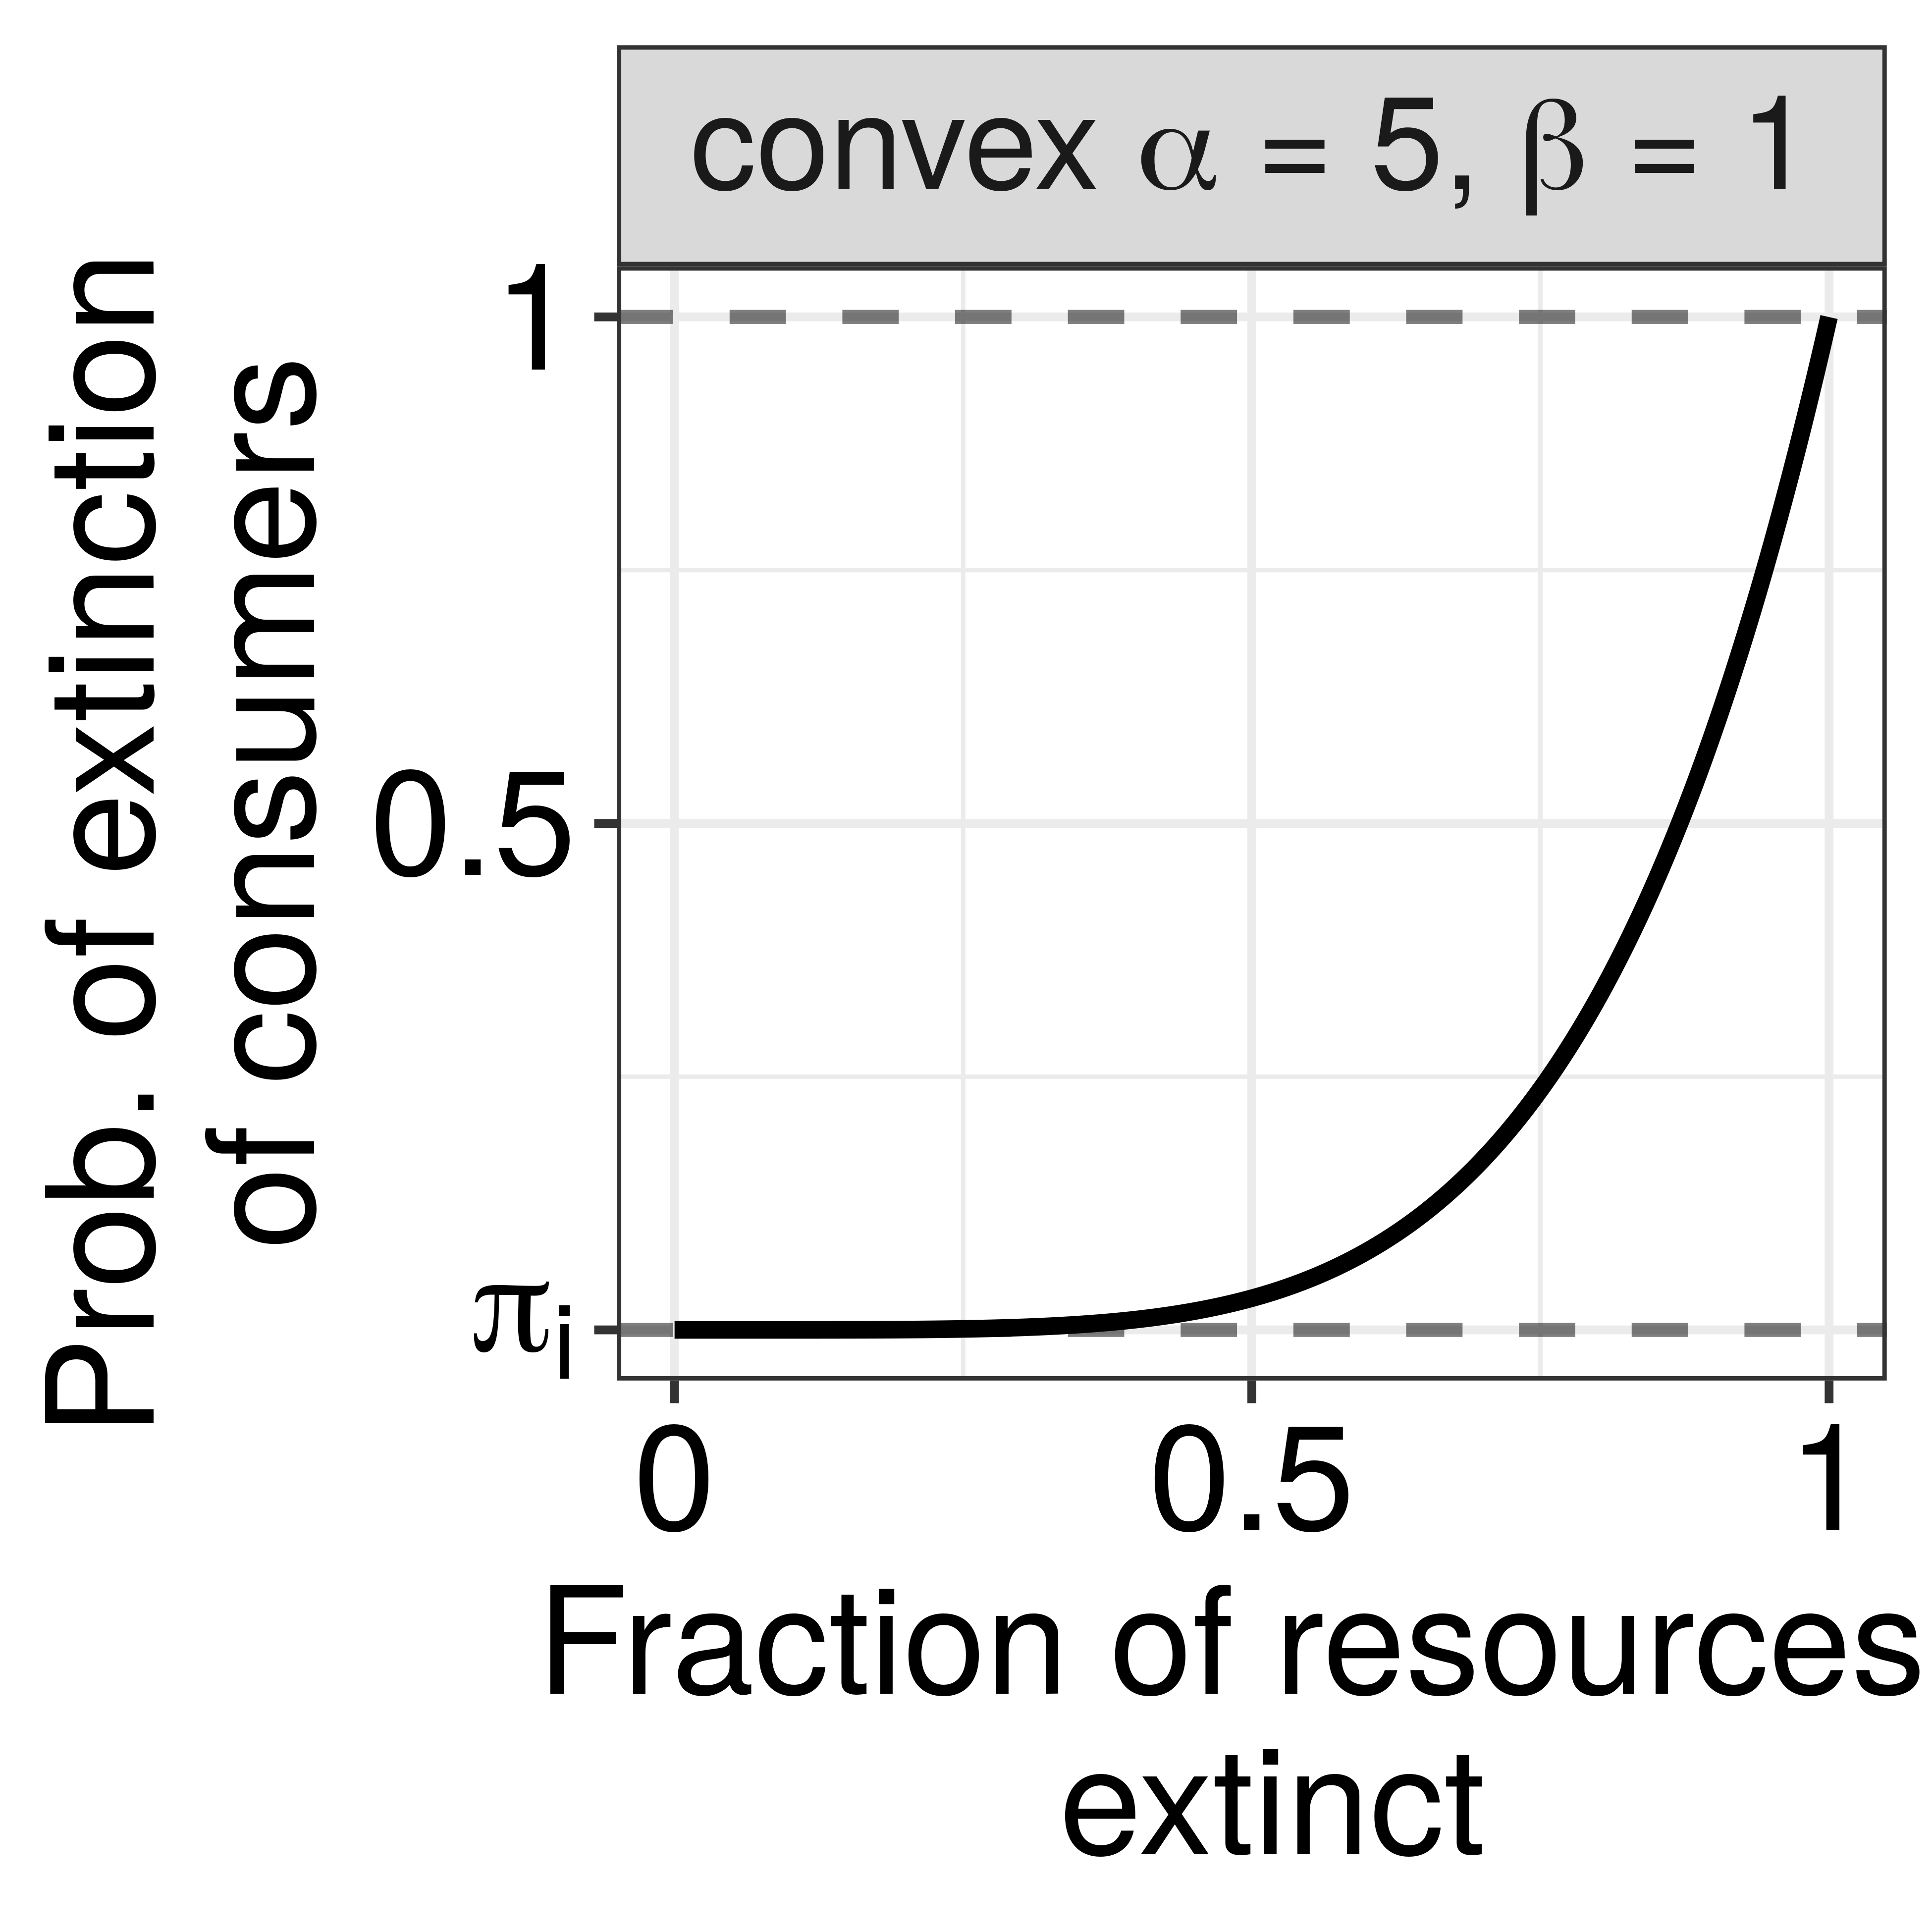
\includegraphics[width=0.19\textwidth,valign=t]{fform_5_1.png}
  \includegraphics[width=0.8\textwidth,valign=t]{lambda_Model_food_web_with_350_consumer_and_50_basal_species_(4)_Not_weighted_basal_5_1.pdf}
  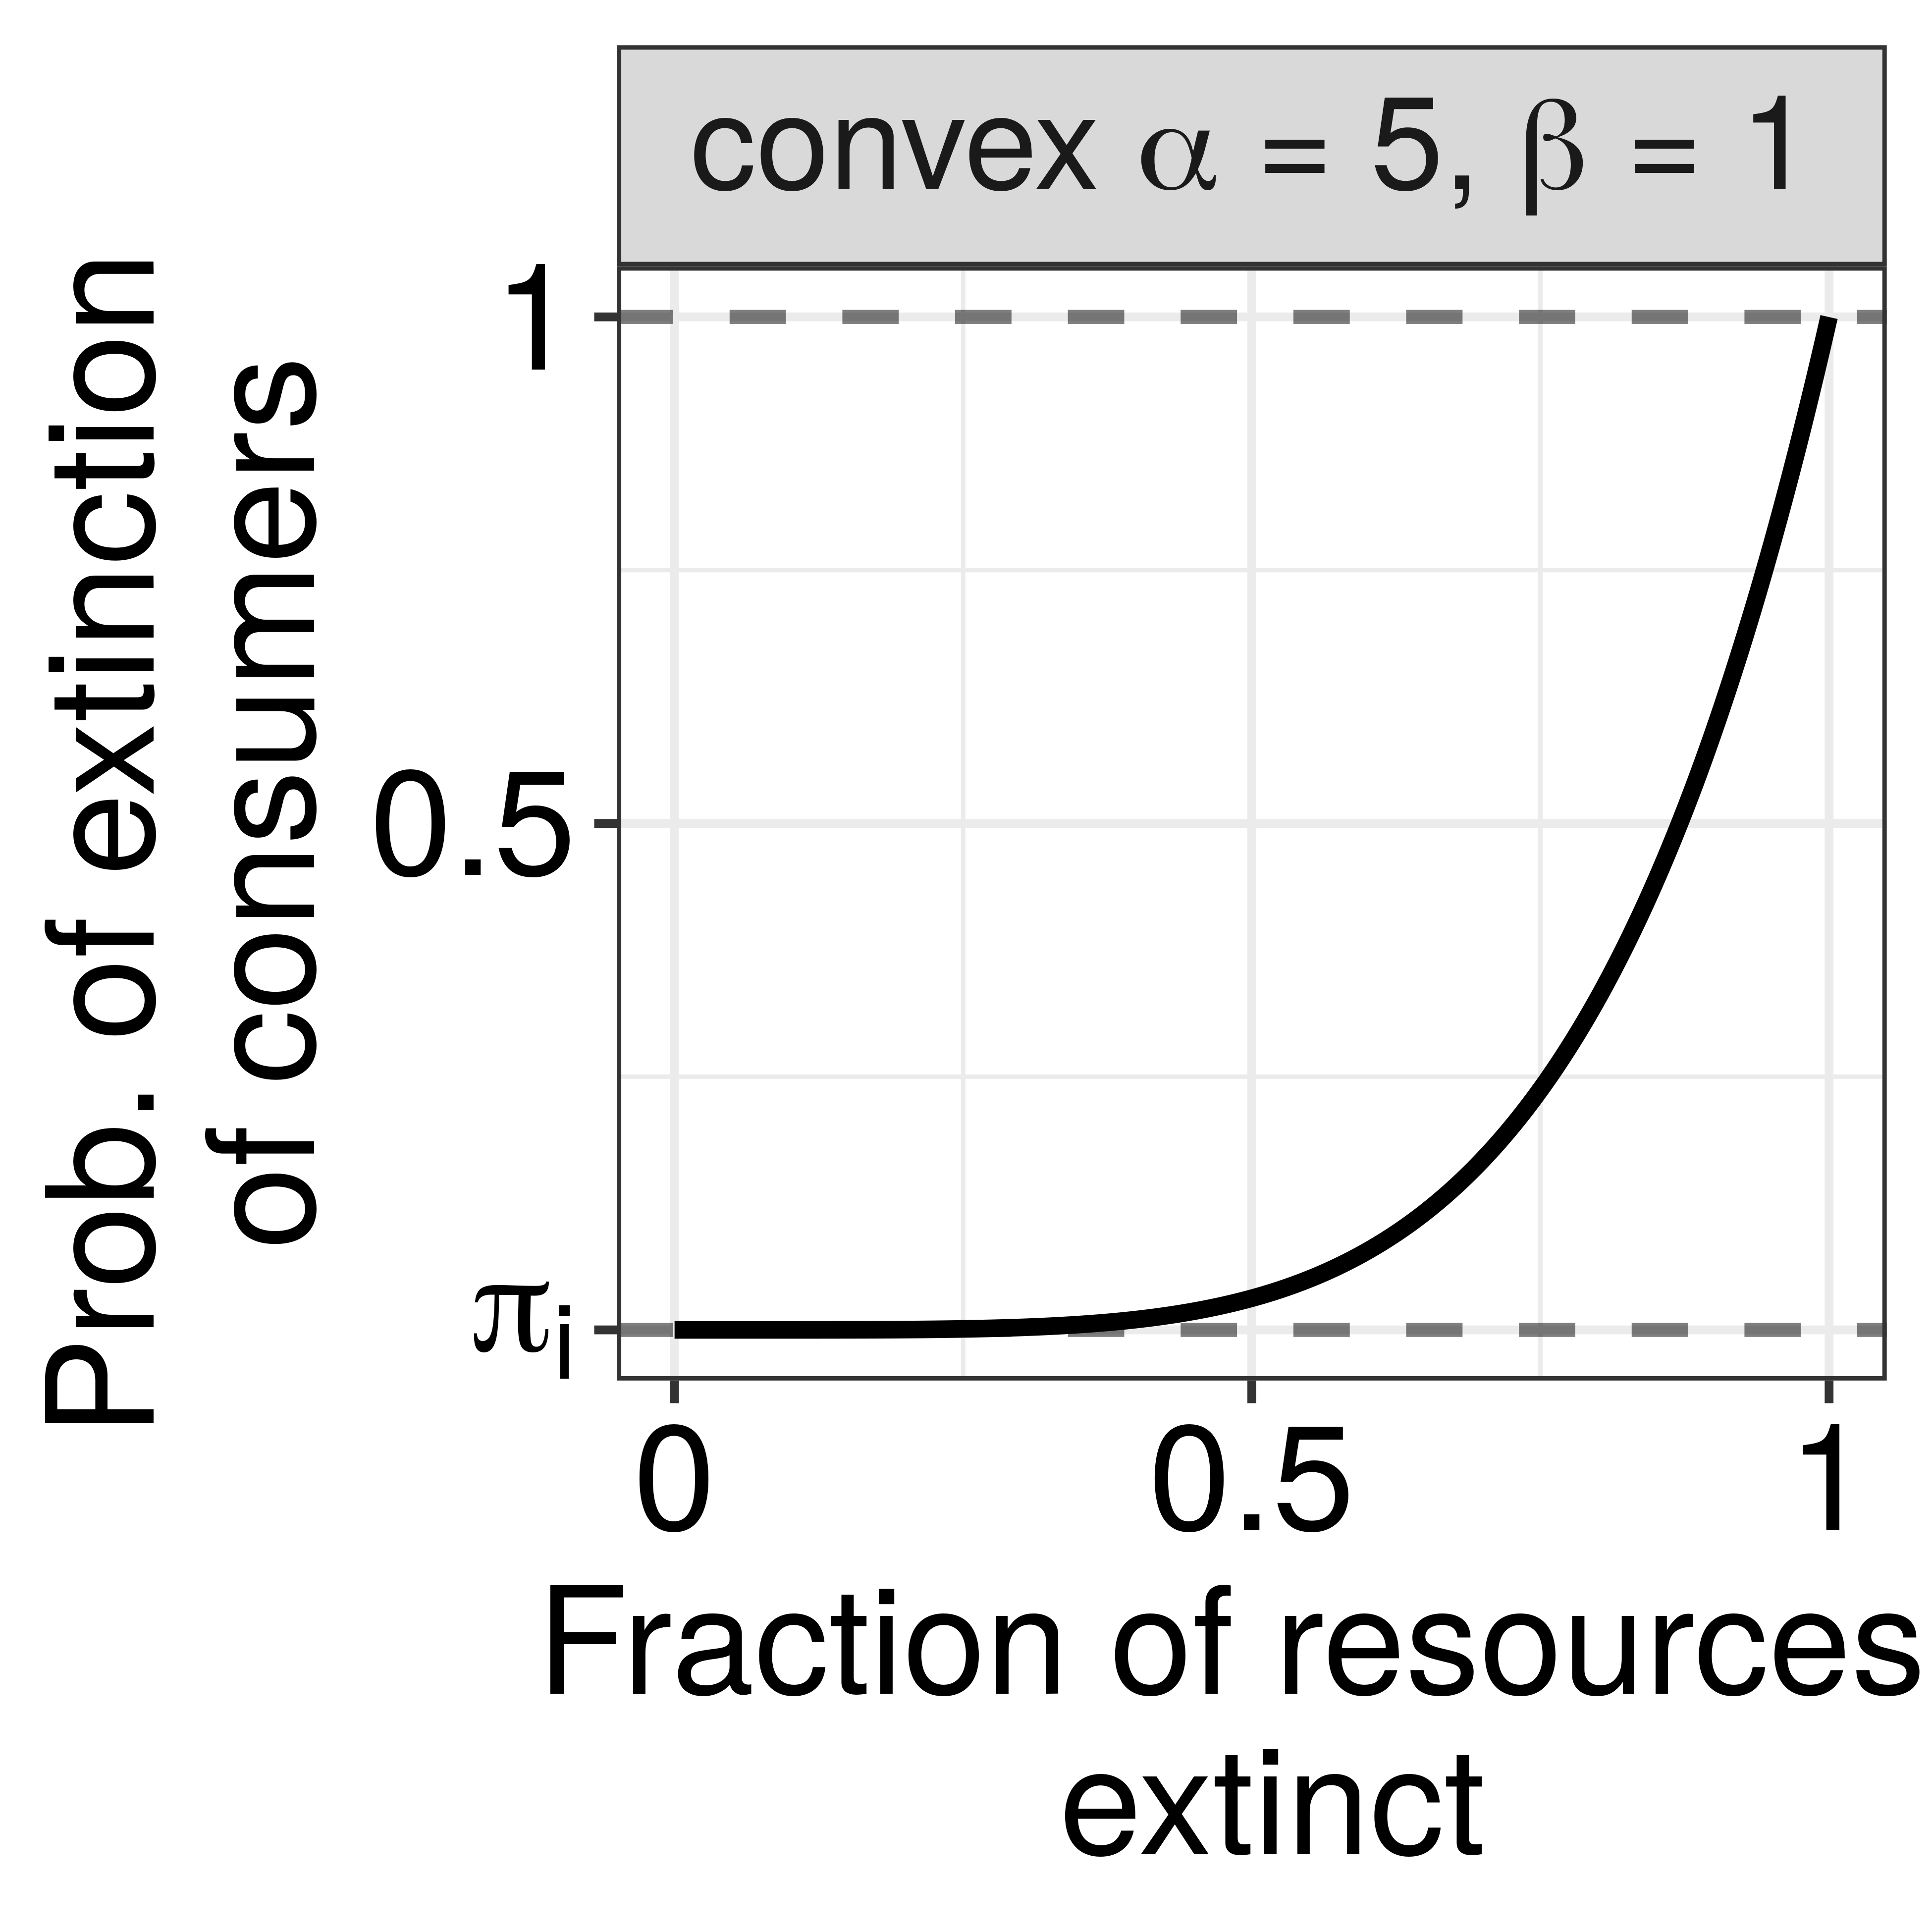
\includegraphics[width=0.19\textwidth,valign=t]{fform_5_1.png}
  \caption{Figure continued.}
  \label{fig:patchloss_web4_51}
\end{figure}

\begin{figure}\ContinuedFloat
  \includegraphics[width=0.8\textwidth,valign=t]{lambda_Model_food_web_with_350_consumer_and_50_basal_species_(4)_Weighted_basal_1_5.pdf}
  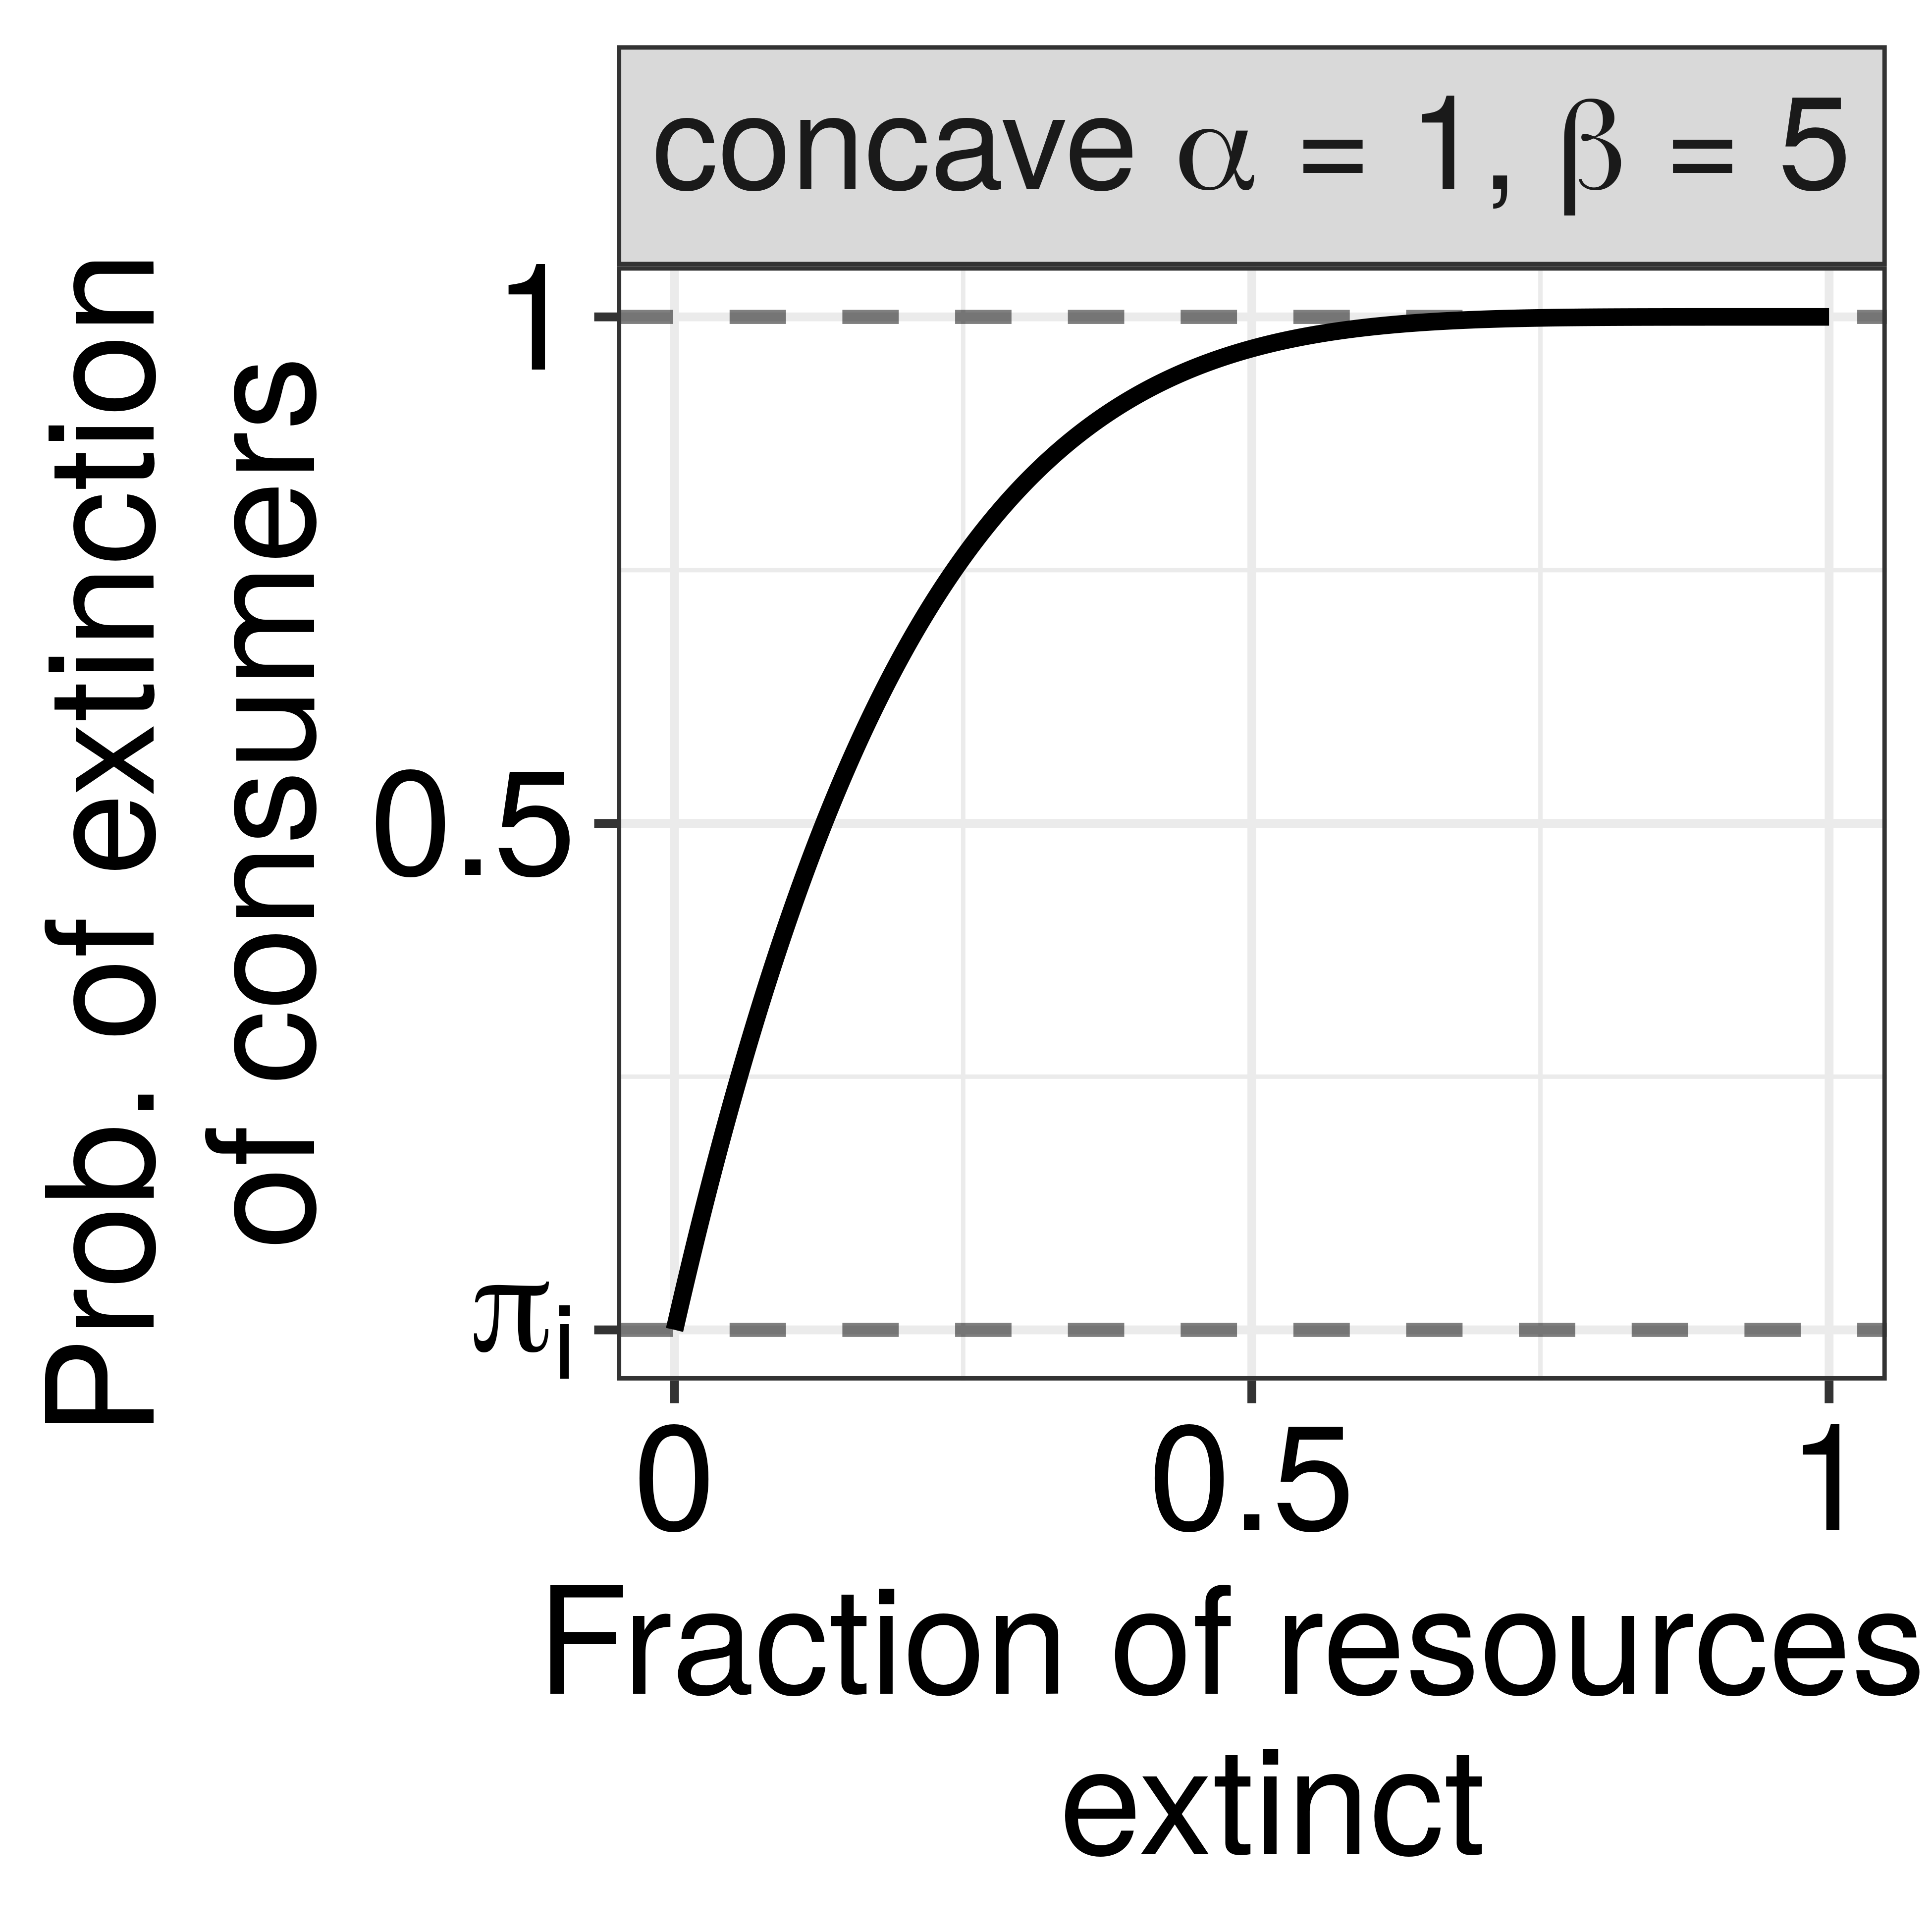
\includegraphics[width=0.19\textwidth,valign=t]{fform_1_5.png}
  \includegraphics[width=0.8\textwidth,valign=t]{lambda_Model_food_web_with_350_consumer_and_50_basal_species_(4)_Not_weighted_basal_1_5.pdf}
  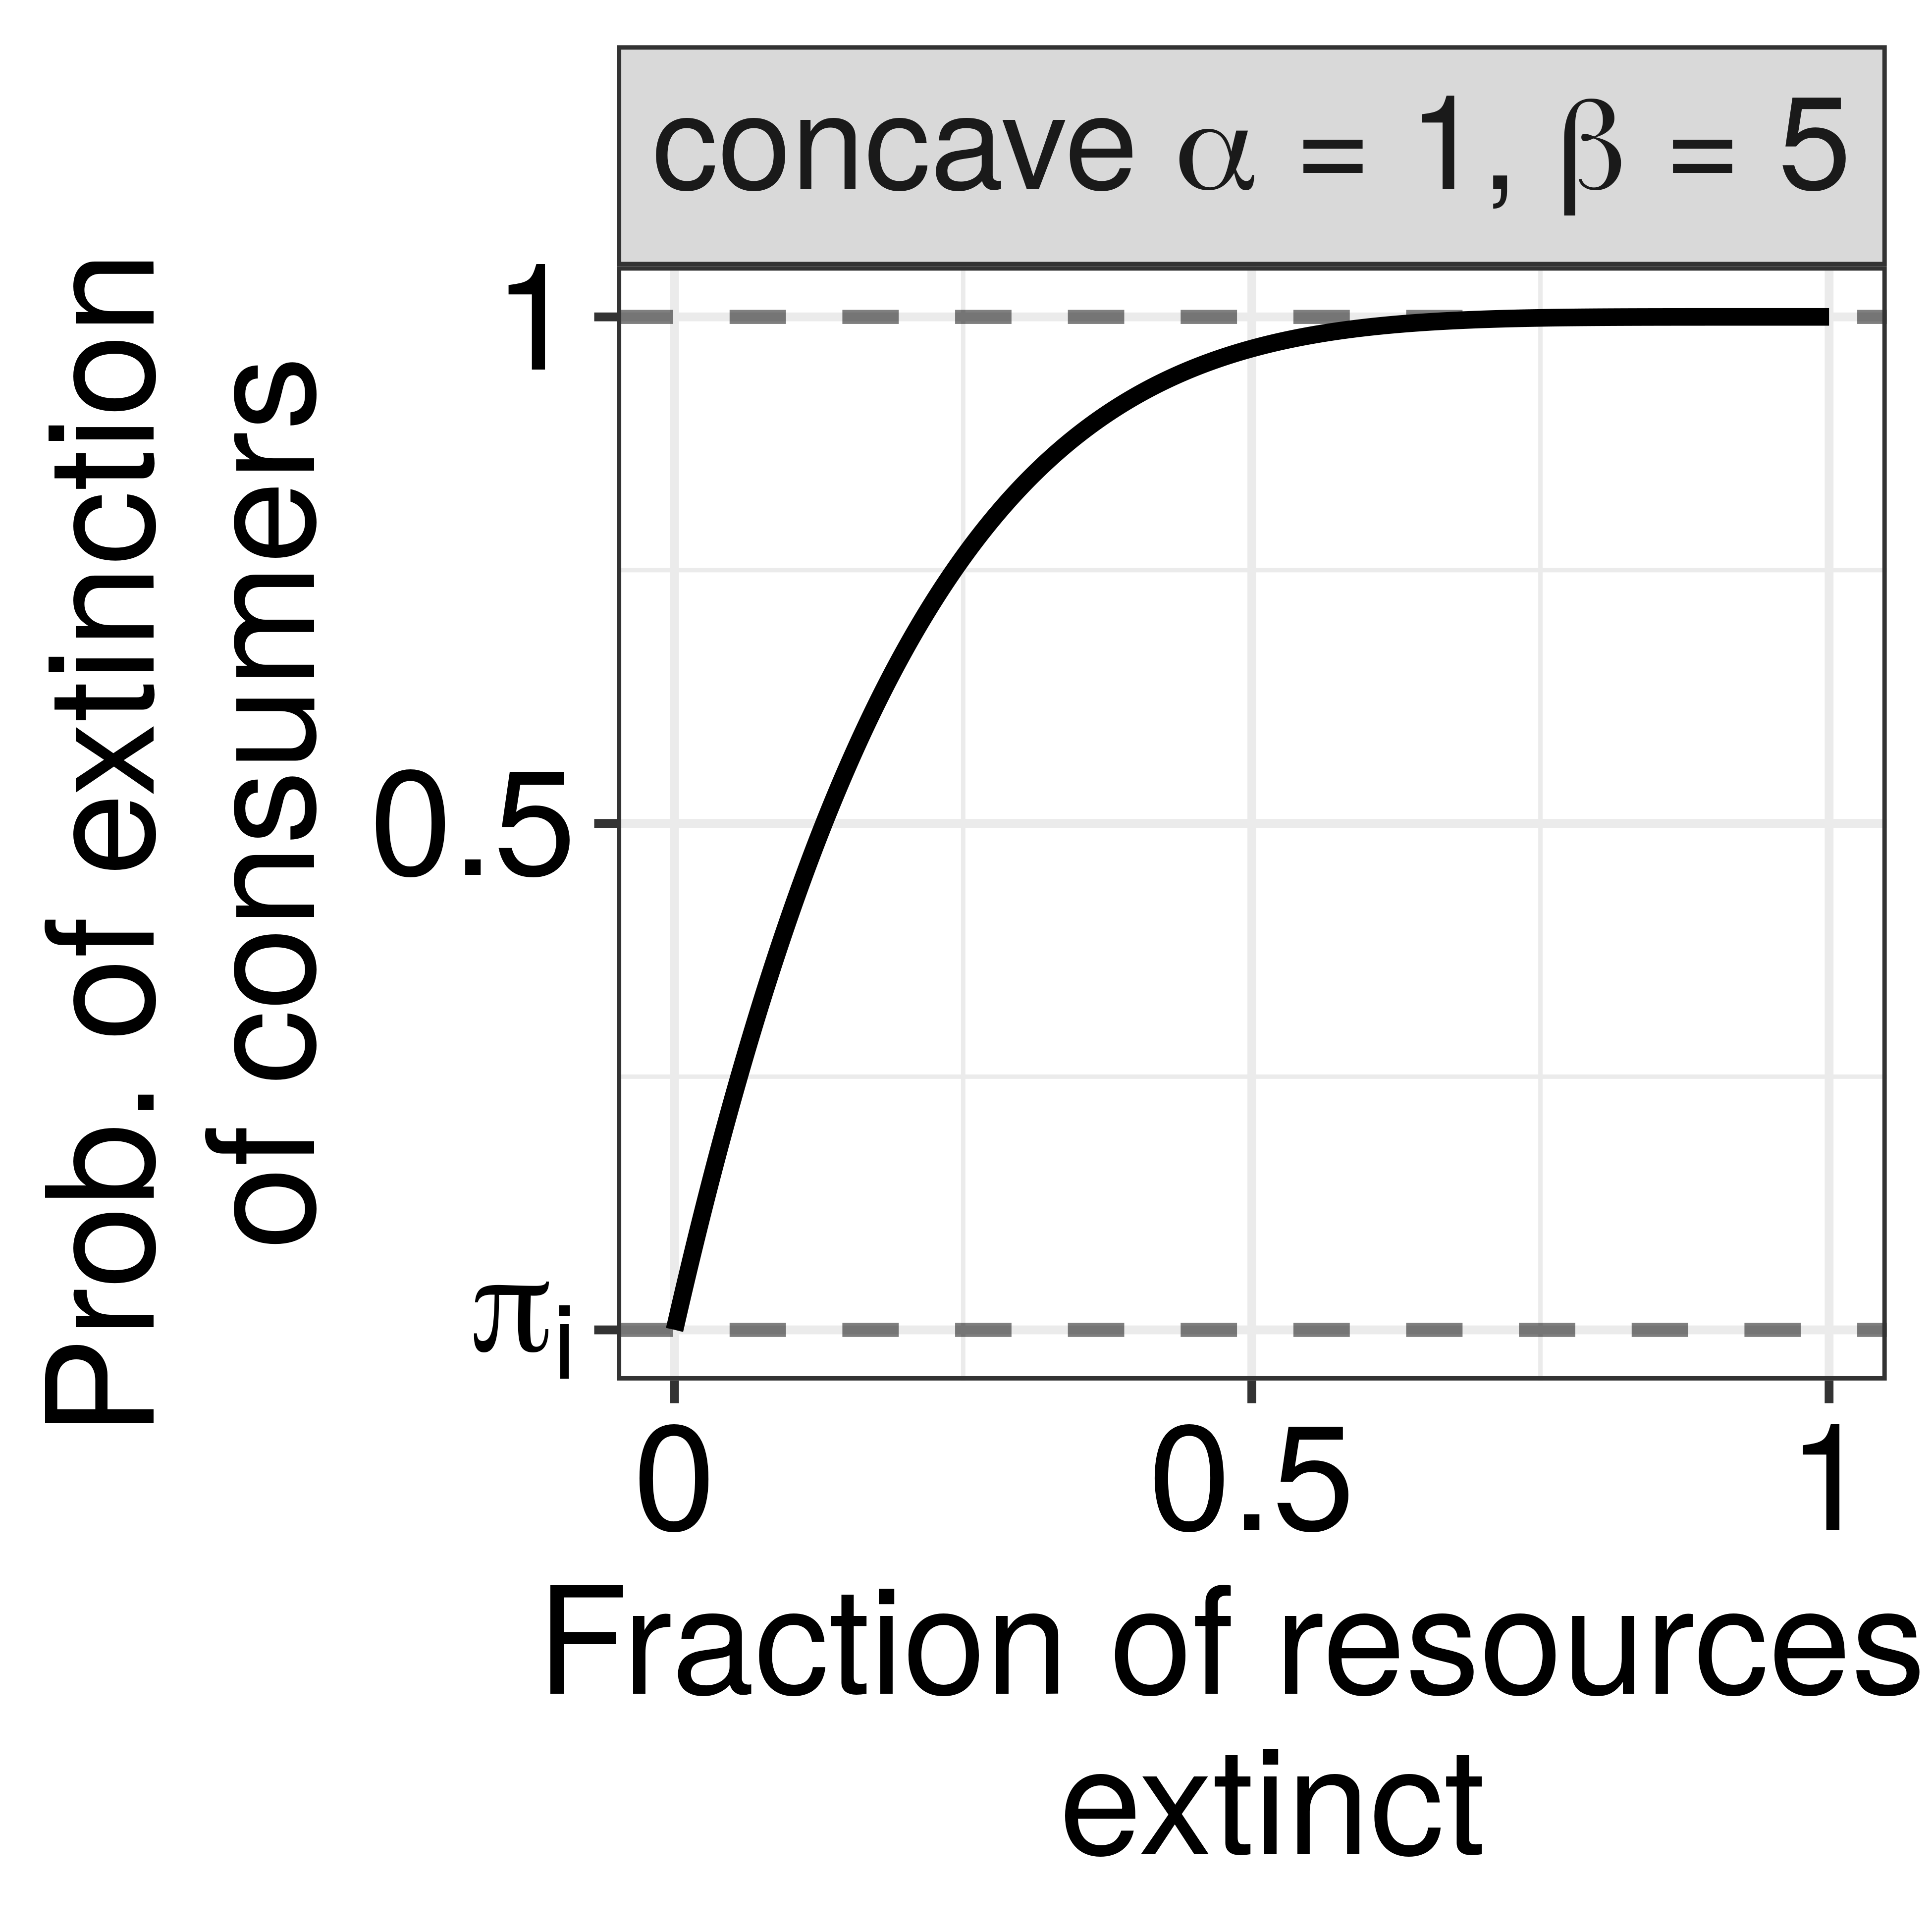
\includegraphics[width=0.19\textwidth,valign=t]{fform_1_5.png}
  \caption{Figure continued.}
  \label{fig:patchloss_web4_15}
\end{figure}

\begin{figure}\ContinuedFloat
  \includegraphics[width=0.8\textwidth,valign=t]{lambda_Model_food_web_with_350_consumer_and_50_basal_species_(3)_Weighted_basal_5_5.pdf}
  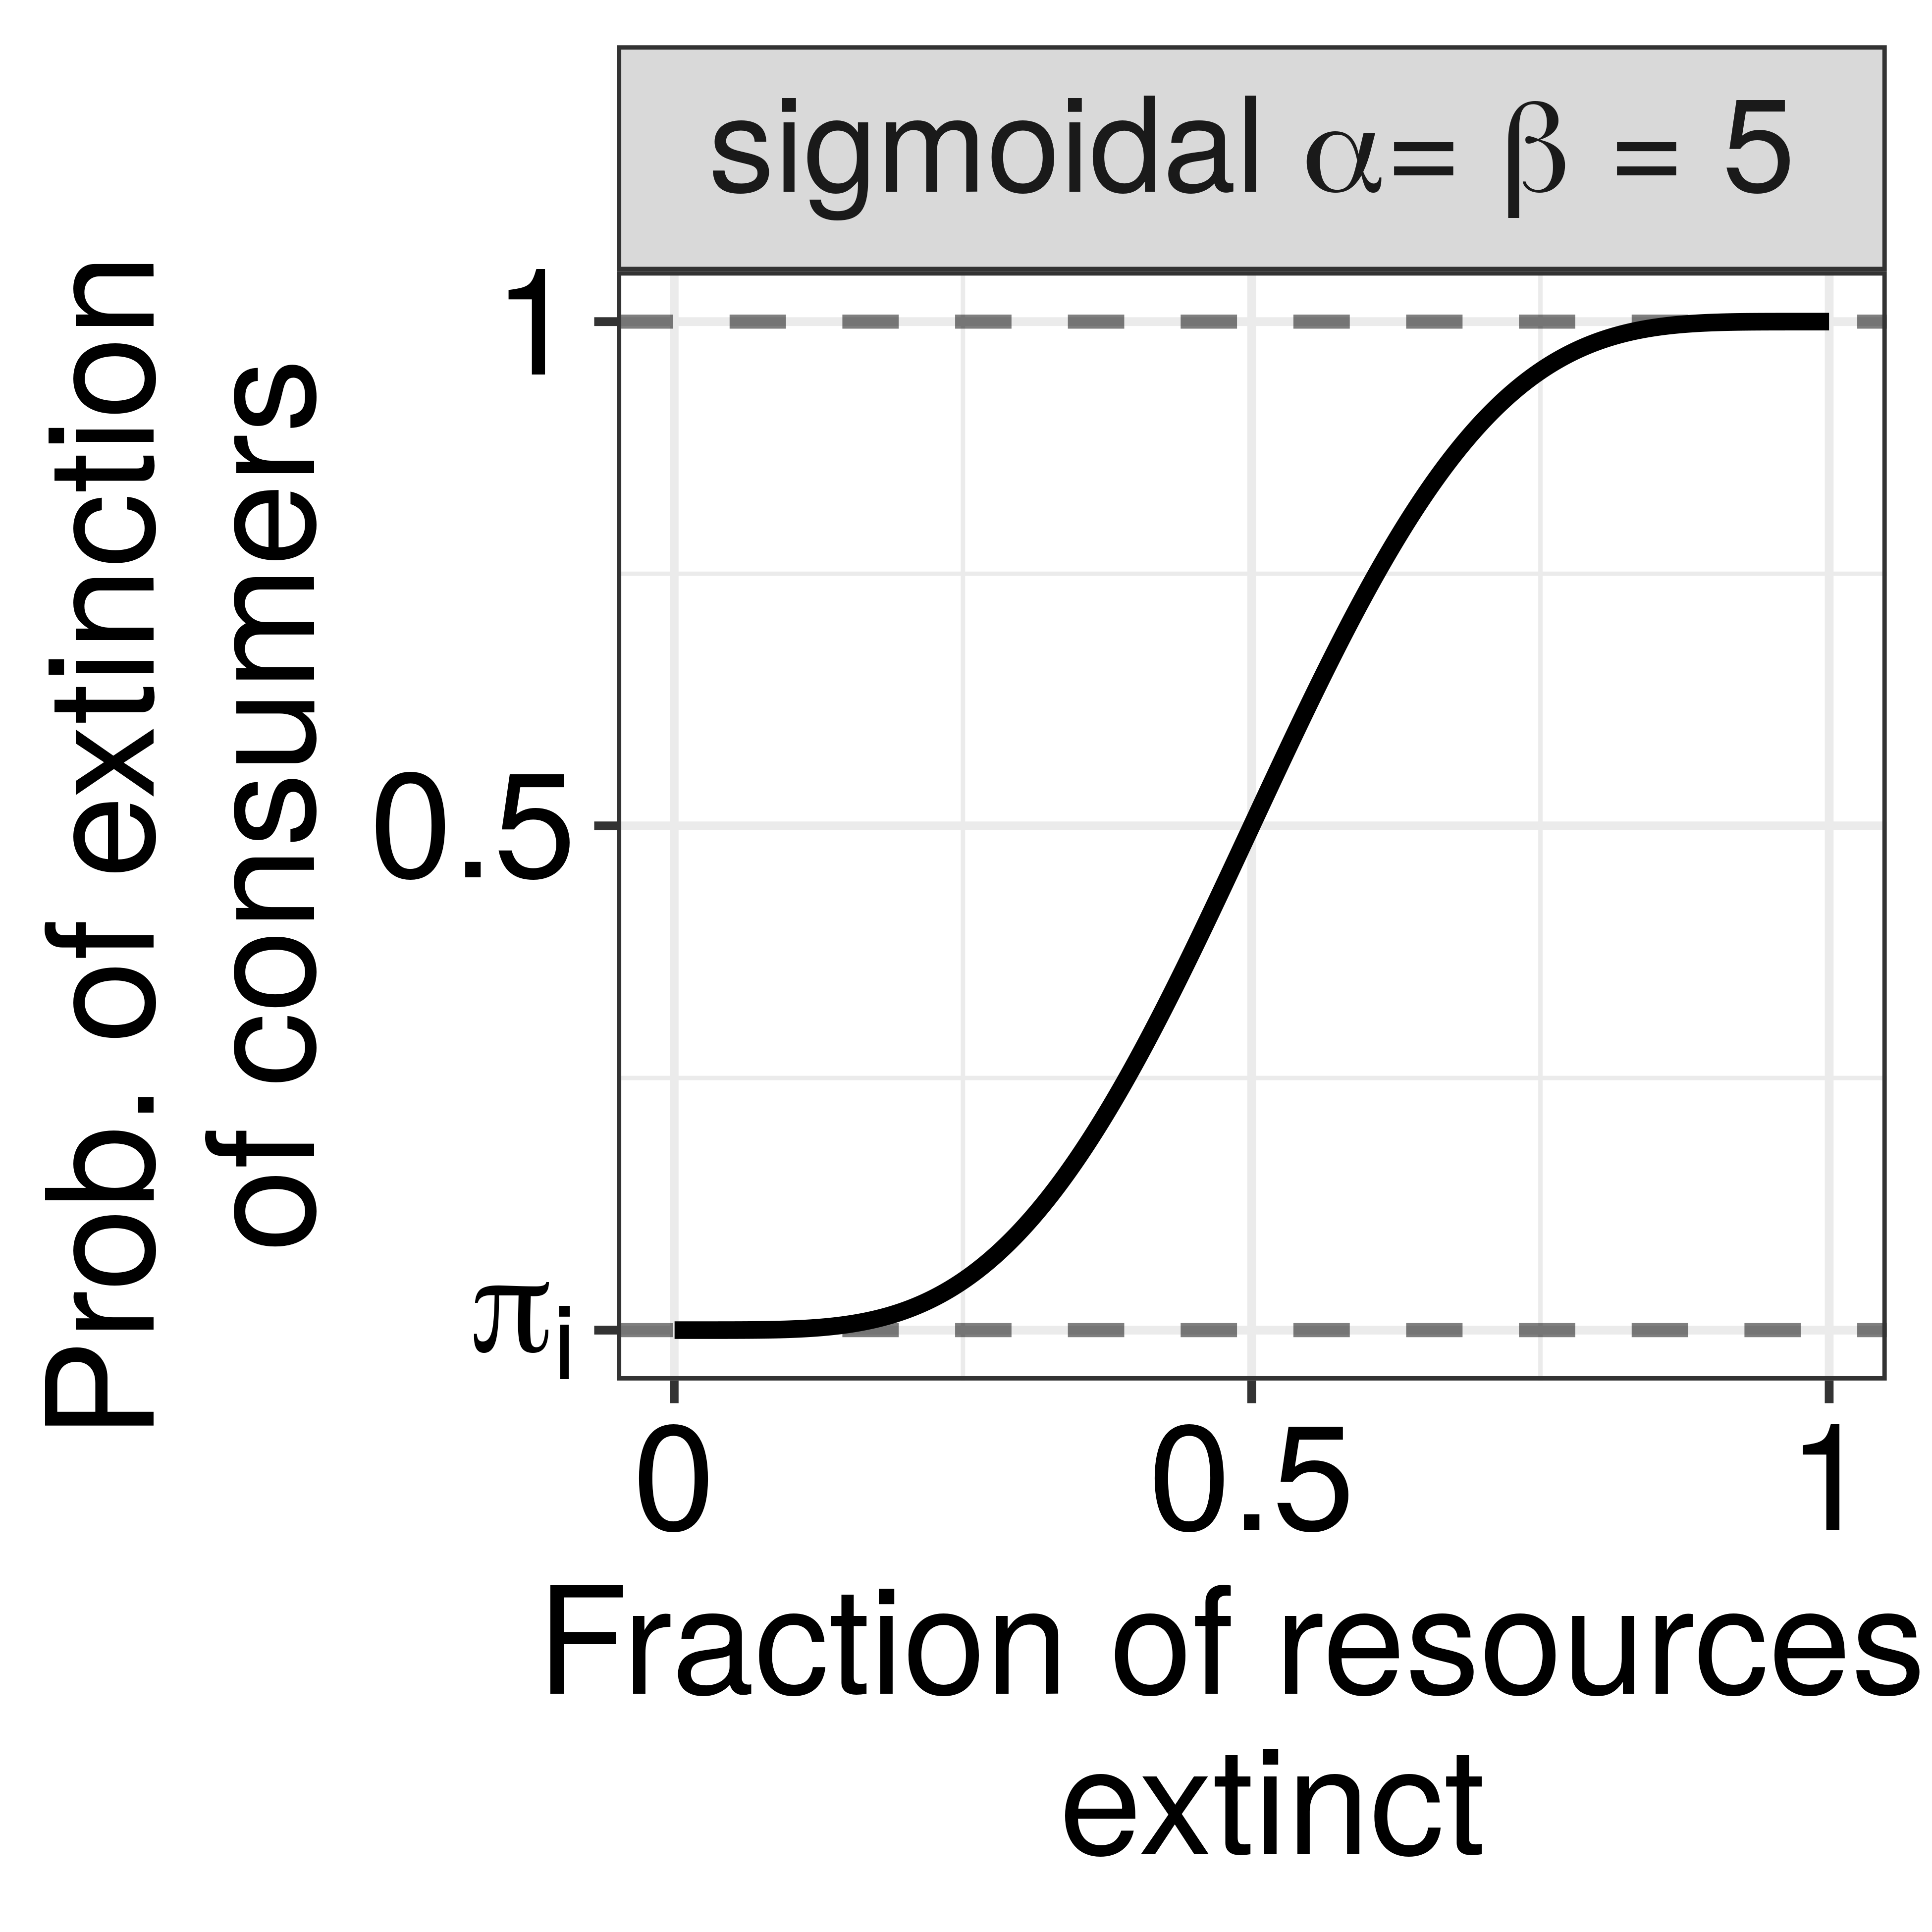
\includegraphics[width=0.19\textwidth,valign=t]{fform_5_5.png}
  \includegraphics[width=0.8\textwidth,valign=t]{lambda_Model_food_web_with_350_consumer_and_50_basal_species_(3)_Not_weighted_basal_5_5.pdf}
  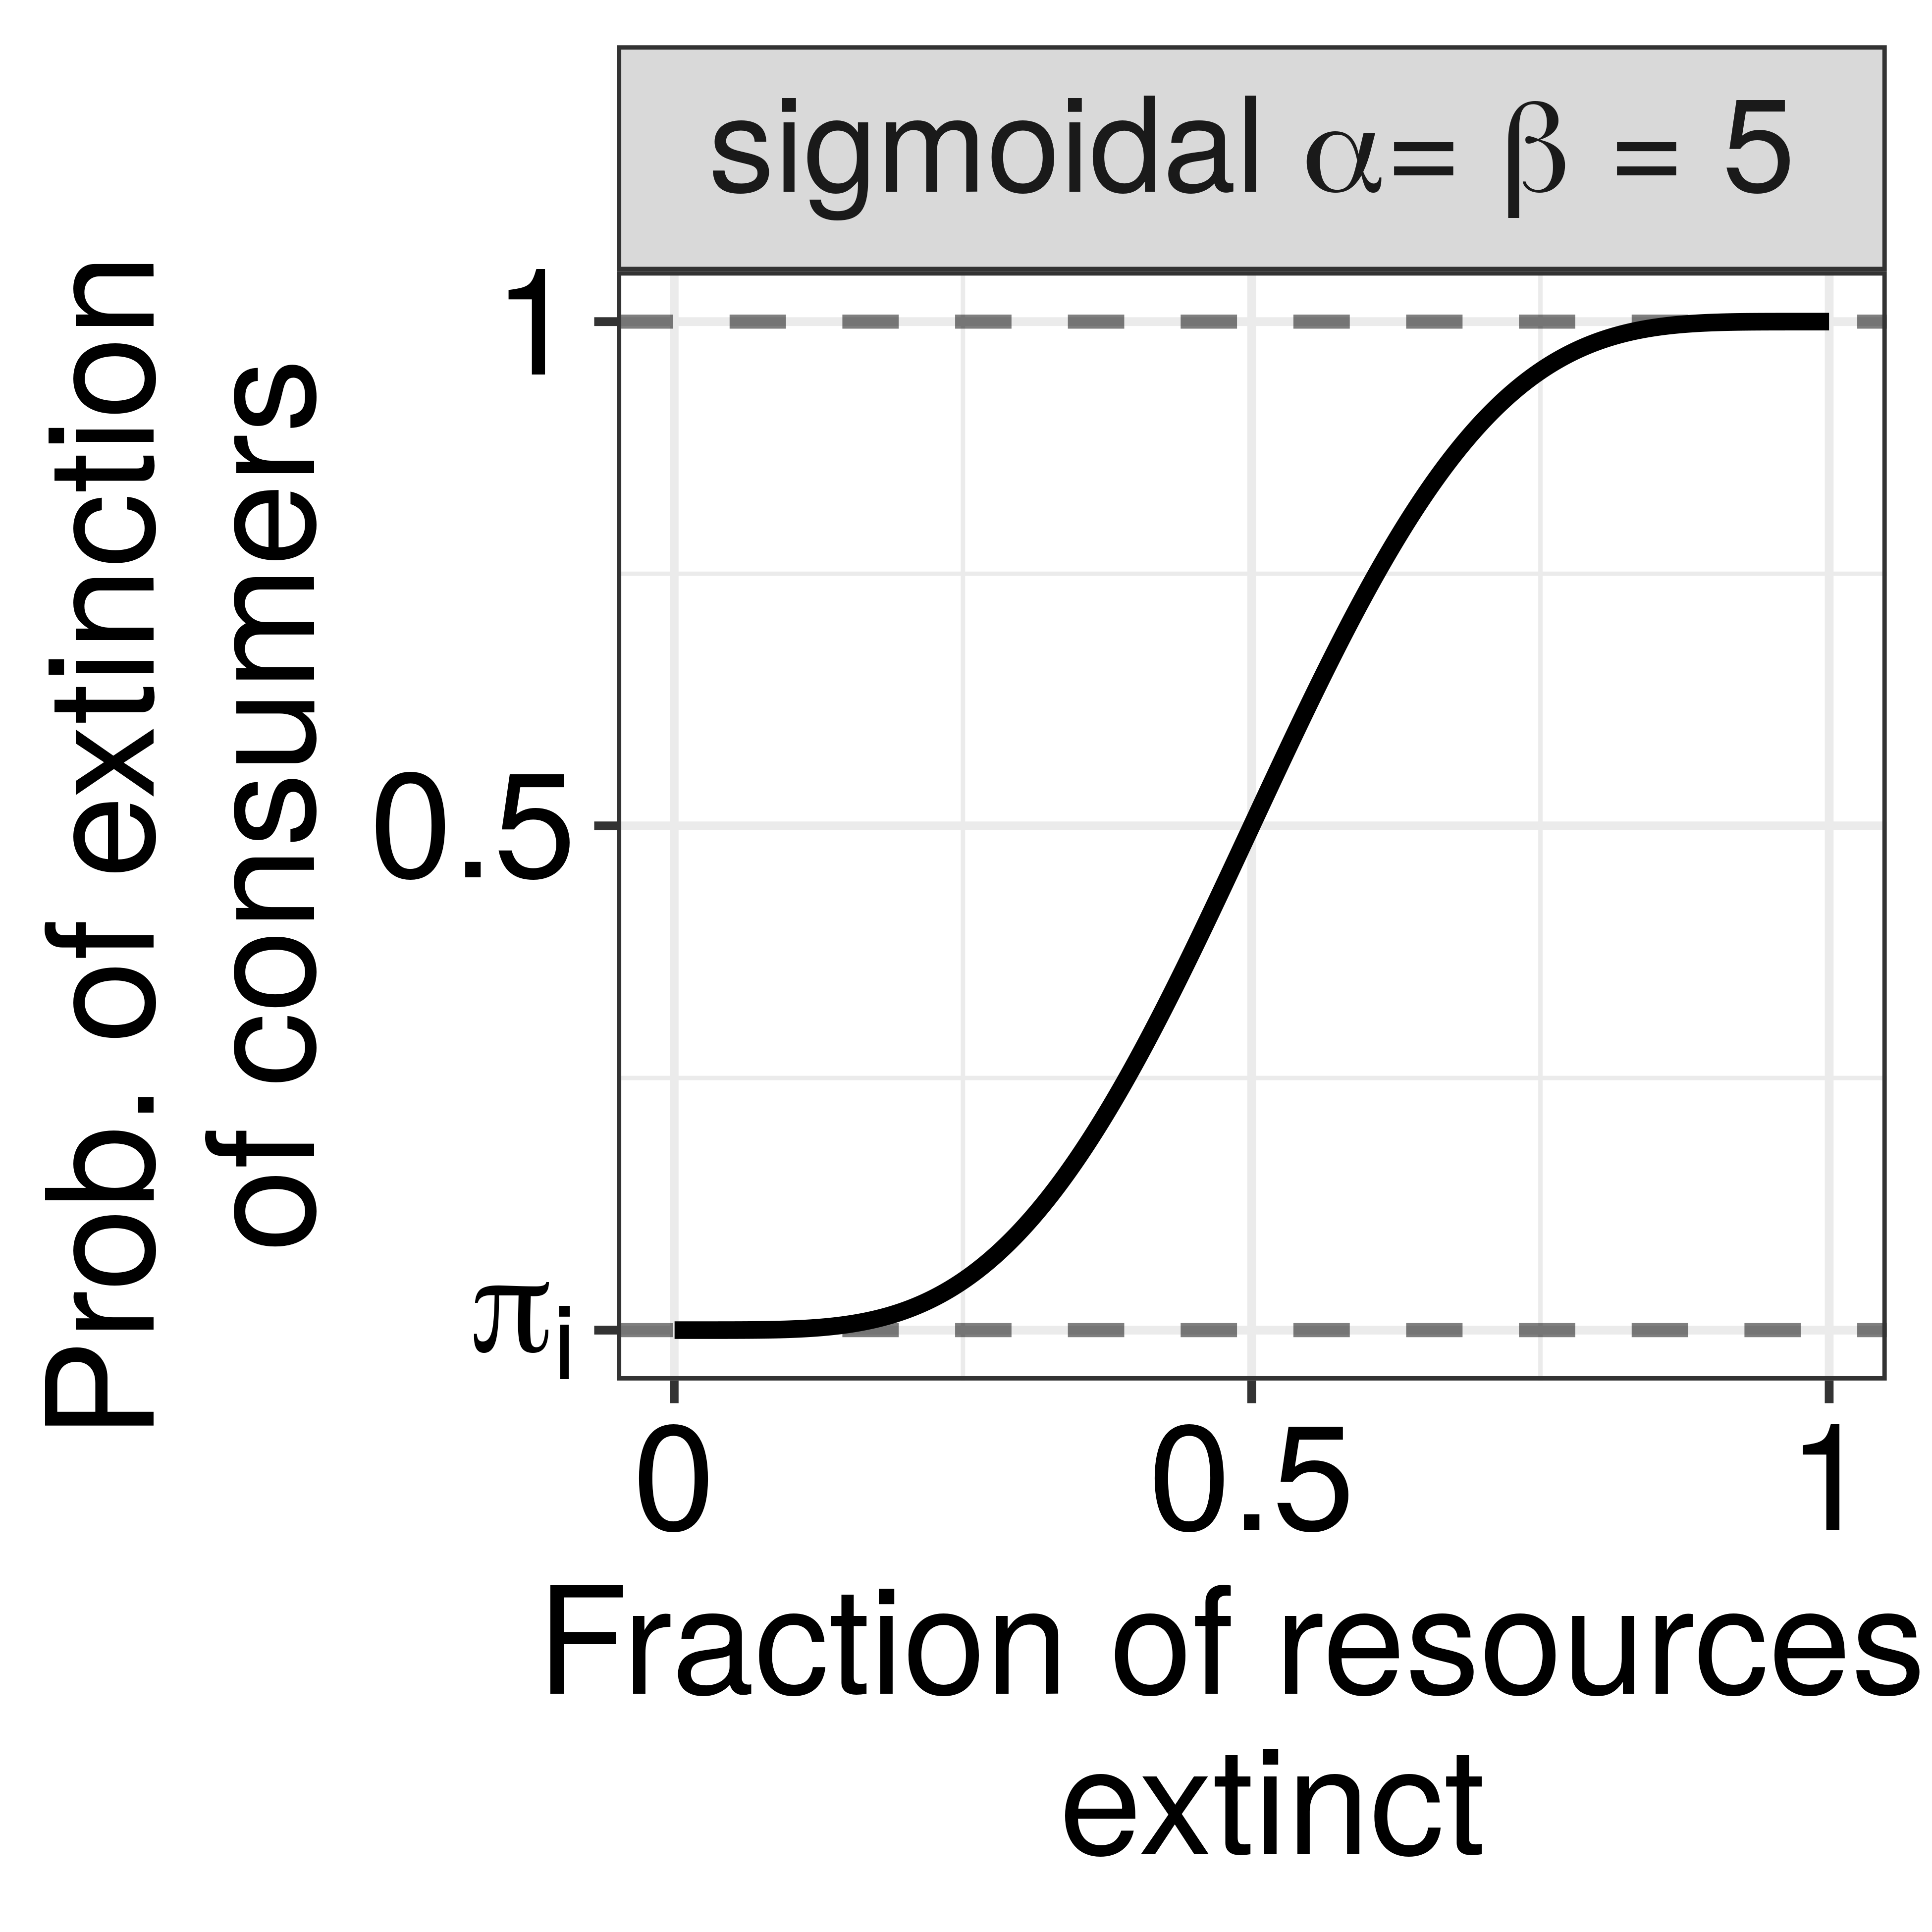
\includegraphics[width=0.19\textwidth,valign=t]{fform_5_5.png}
  \caption{Figure continued.}
  \label{fig:patchloss_web4_55}
\end{figure}

\begin{figure}
  \includegraphics[width=0.8\textwidth,valign=t]{lambda_Model_food_web_with_350_consumer_and_50_basal_species_(5)_Weighted_basal_1_1.pdf}
  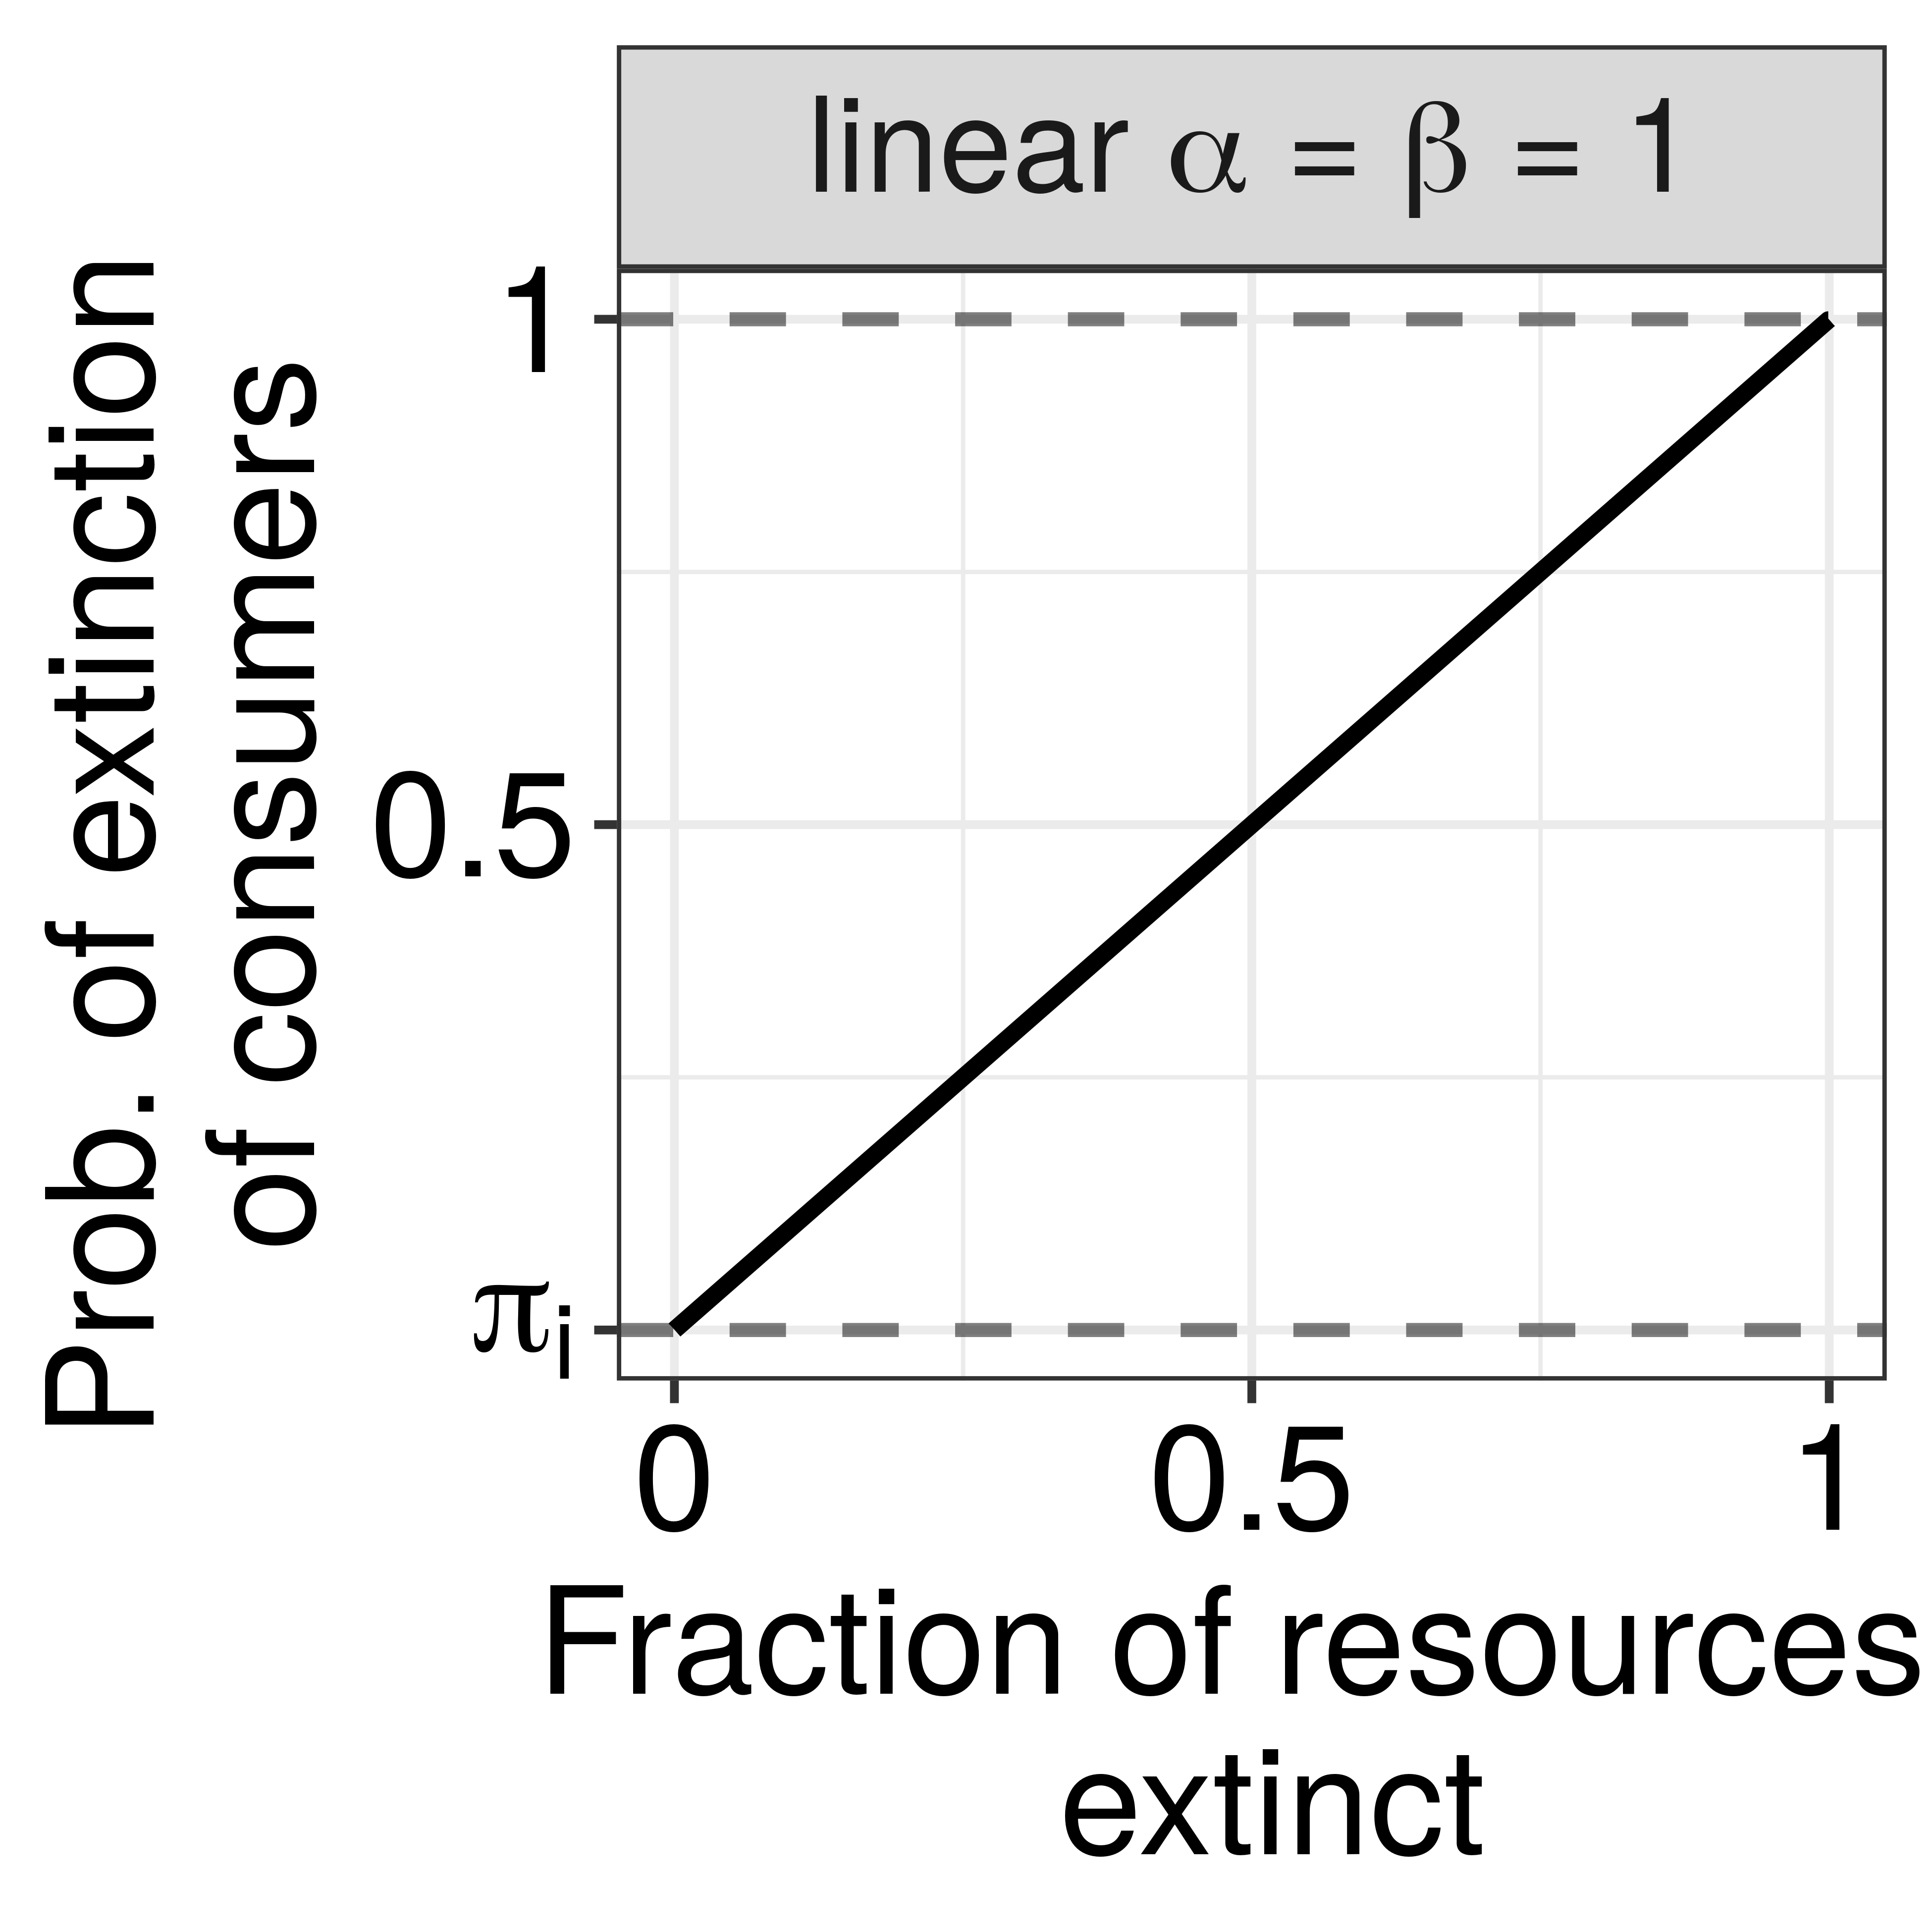
\includegraphics[width=0.19\textwidth,valign=t]{fform_1_1.png}
  \includegraphics[width=0.8\textwidth,valign=t]{lambda_Model_food_web_with_350_consumer_and_50_basal_species_(5)_Not_weighted_basal_1_1.pdf}
  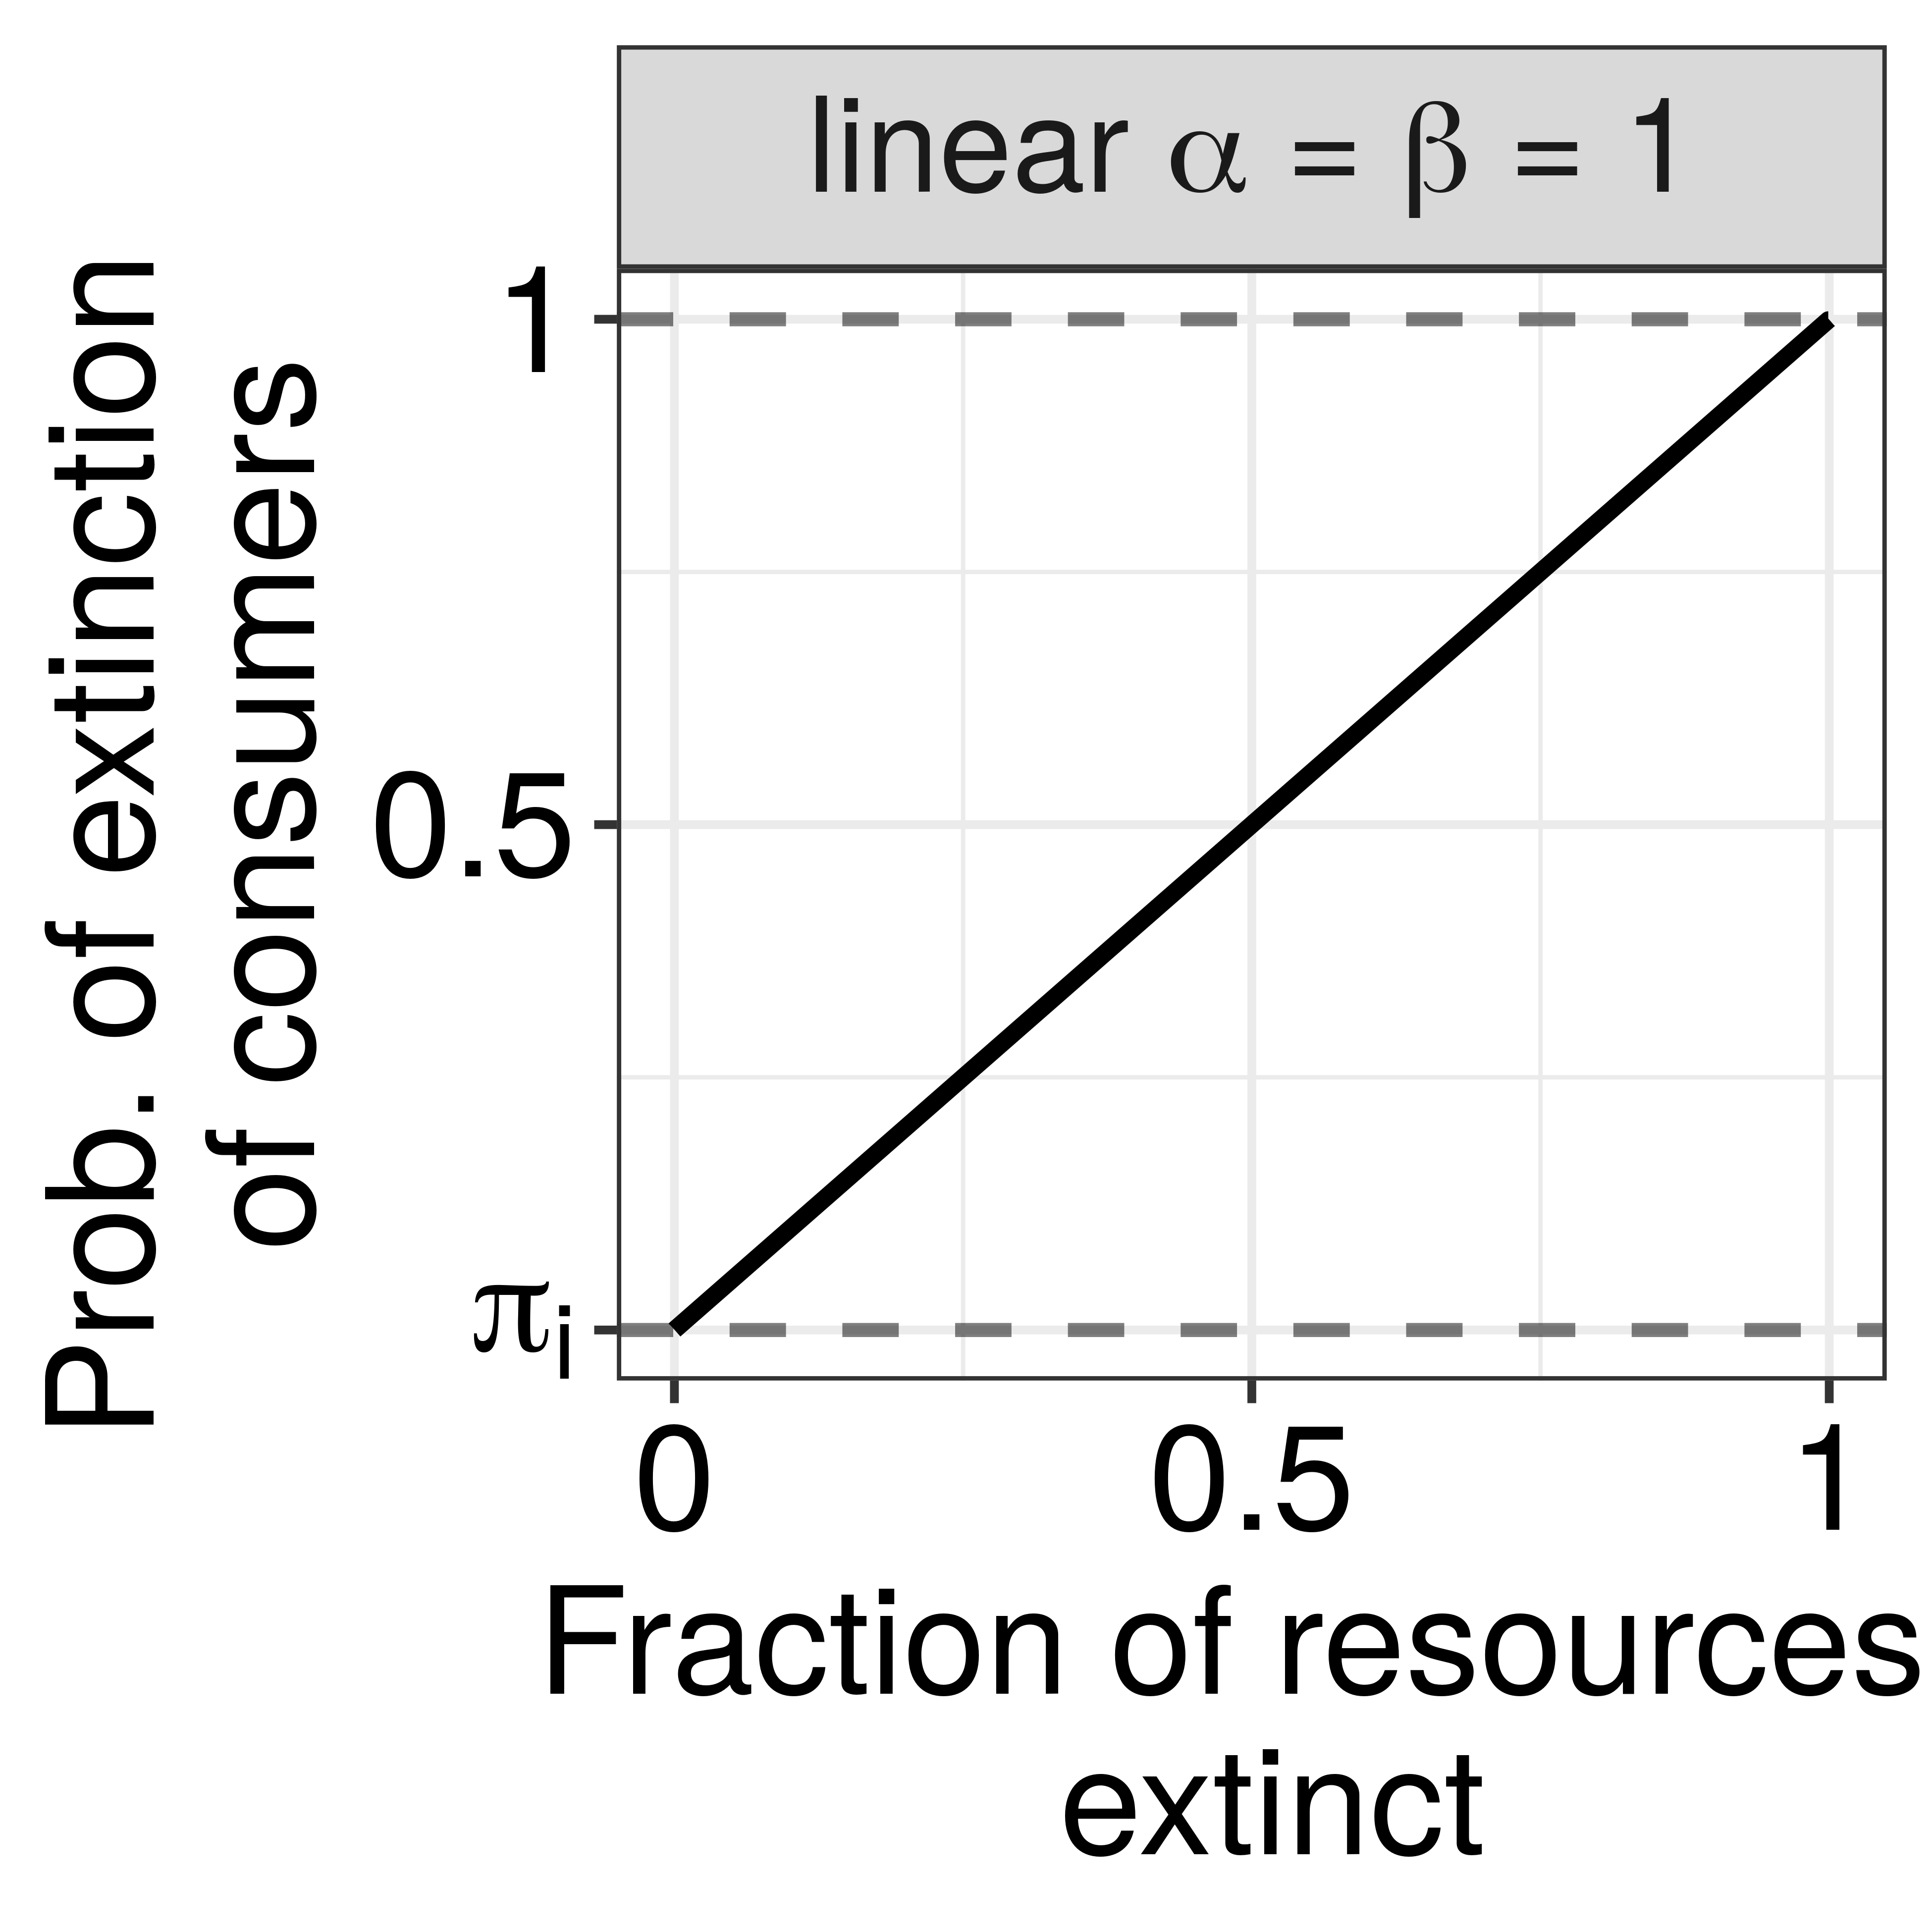
\includegraphics[width=0.19\textwidth,valign=t]{fform_1_1.png}
  \caption{As Figure~\ref{fig:patchloss_web1_11}.}
  \label{fig:patchloss_web5_11}
\end{figure}

\begin{figure}\ContinuedFloat
  \includegraphics[width=0.8\textwidth,valign=t]{lambda_Model_food_web_with_350_consumer_and_50_basal_species_(5)_Weighted_basal_5_1.pdf}
  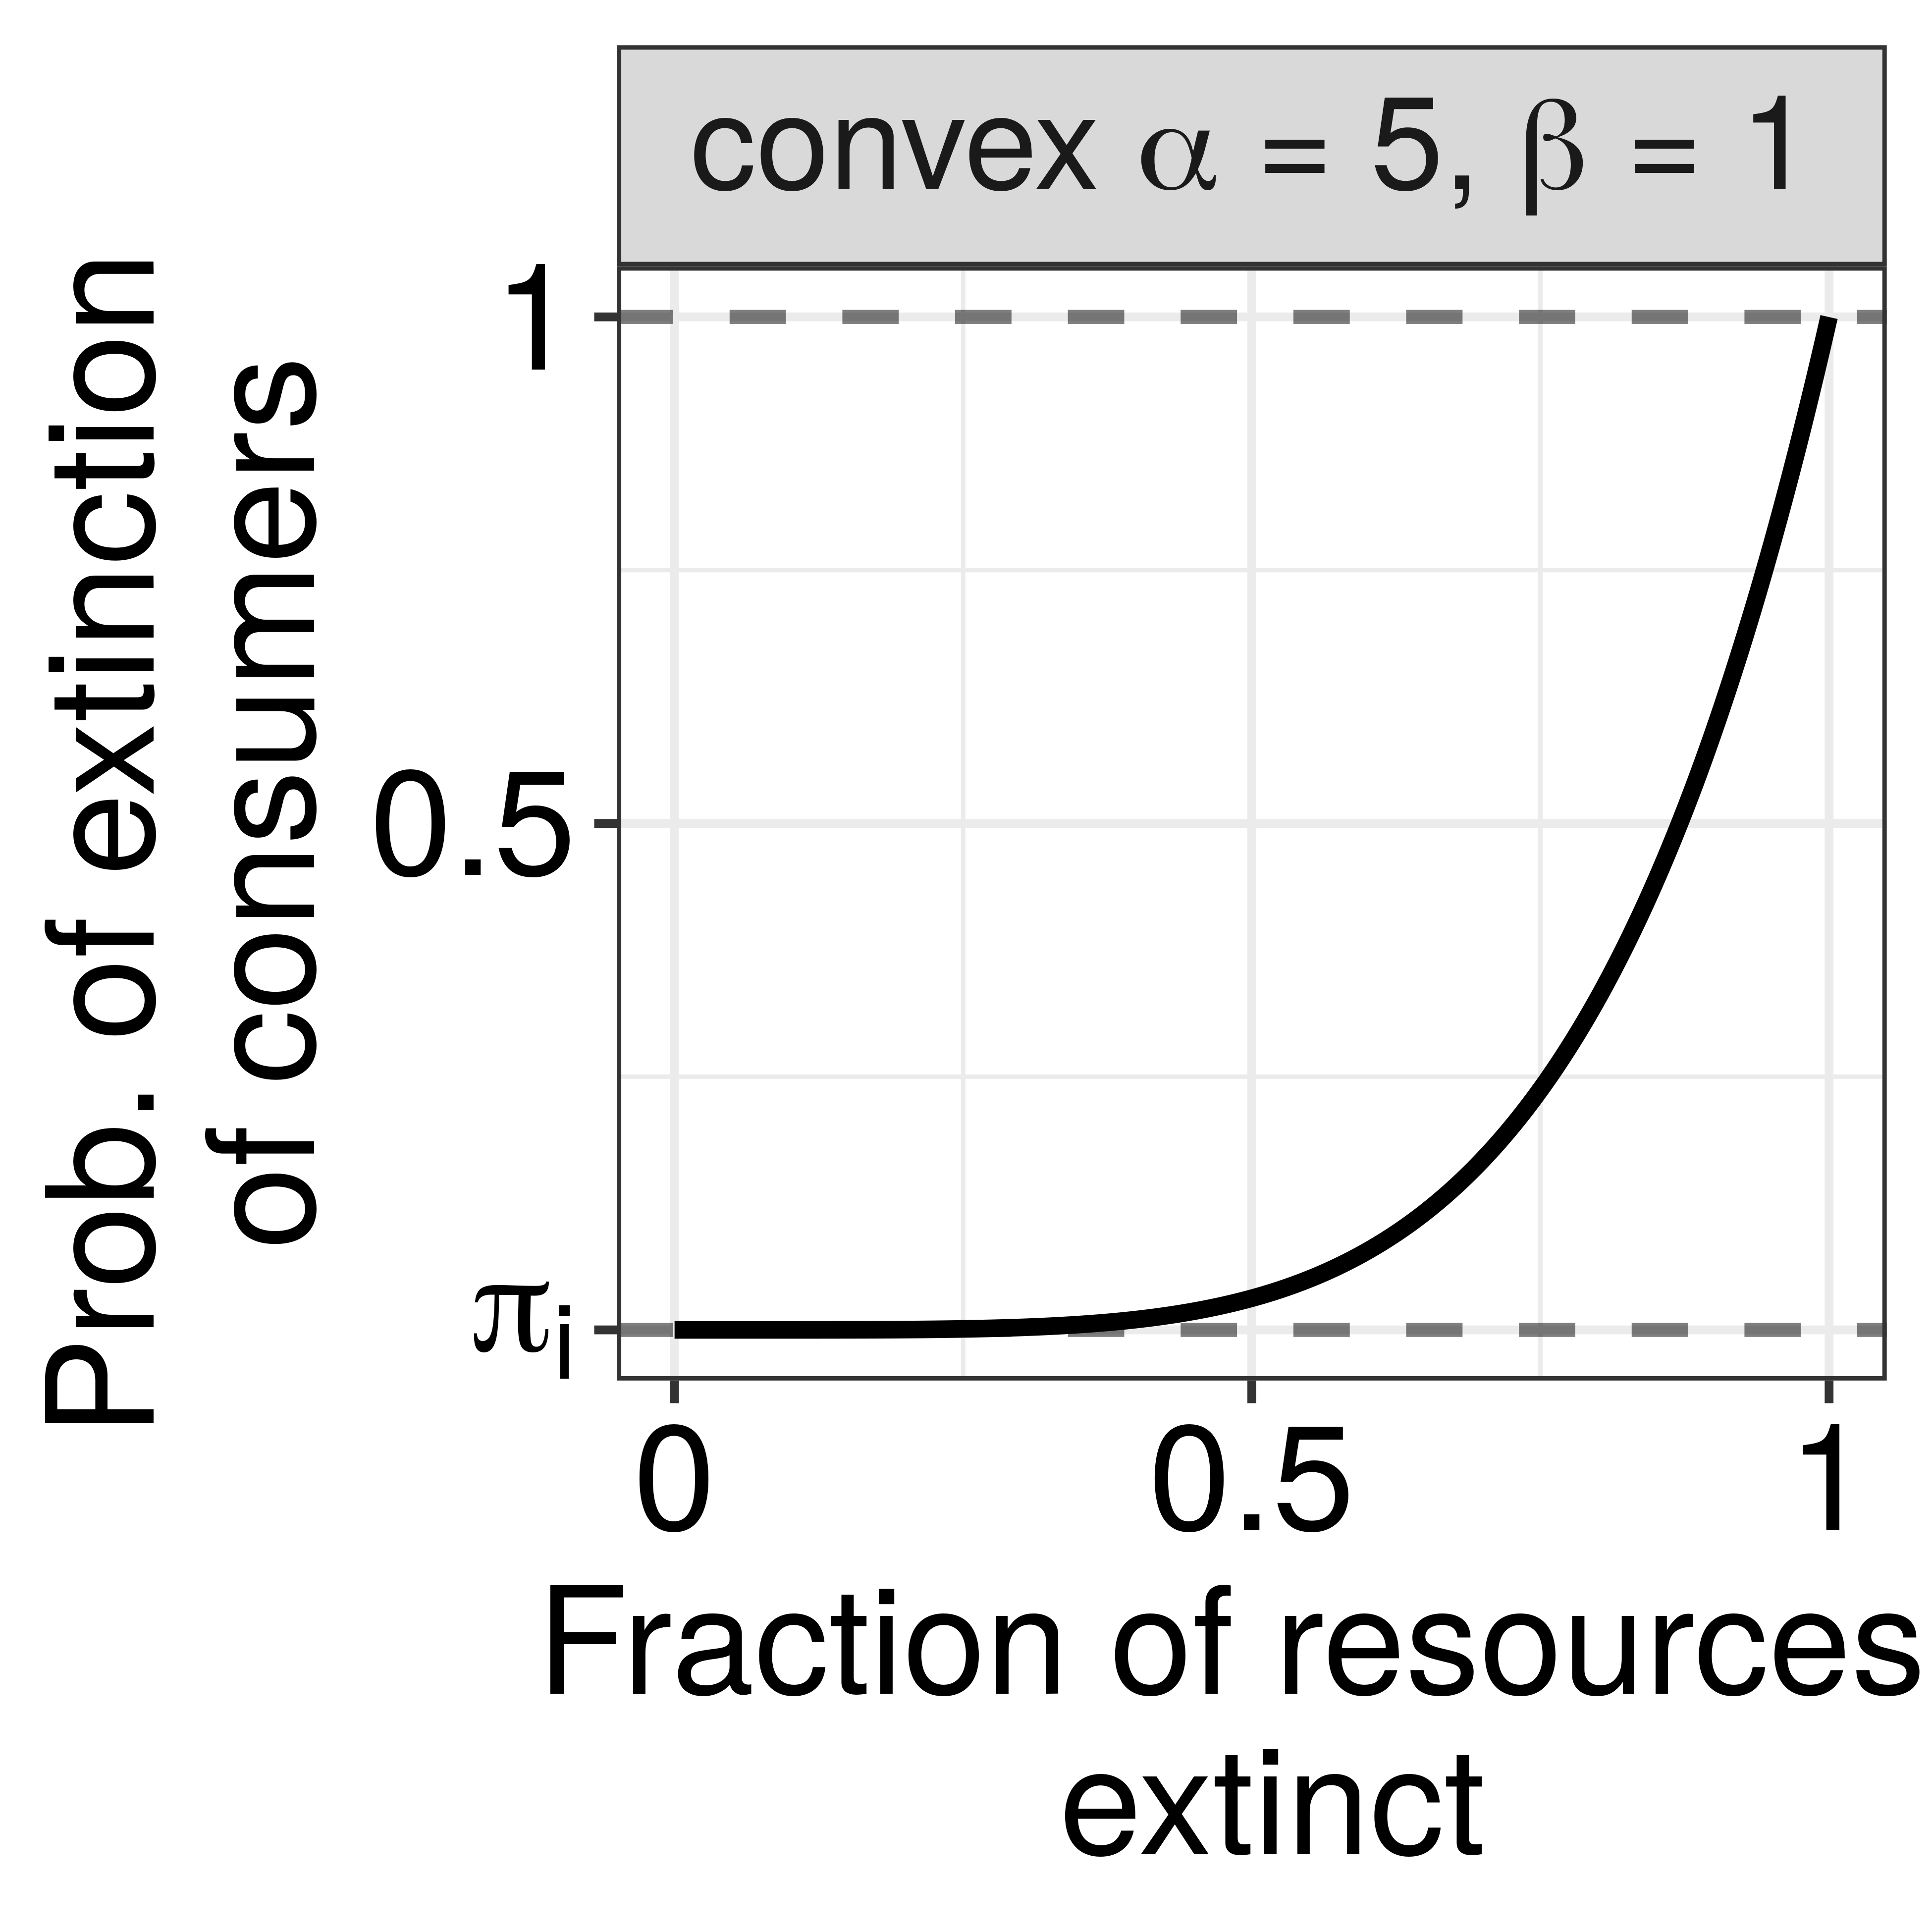
\includegraphics[width=0.19\textwidth,valign=t]{fform_5_1.png}
  \includegraphics[width=0.8\textwidth,valign=t]{lambda_Model_food_web_with_350_consumer_and_50_basal_species_(5)_Not_weighted_basal_5_1.pdf}
  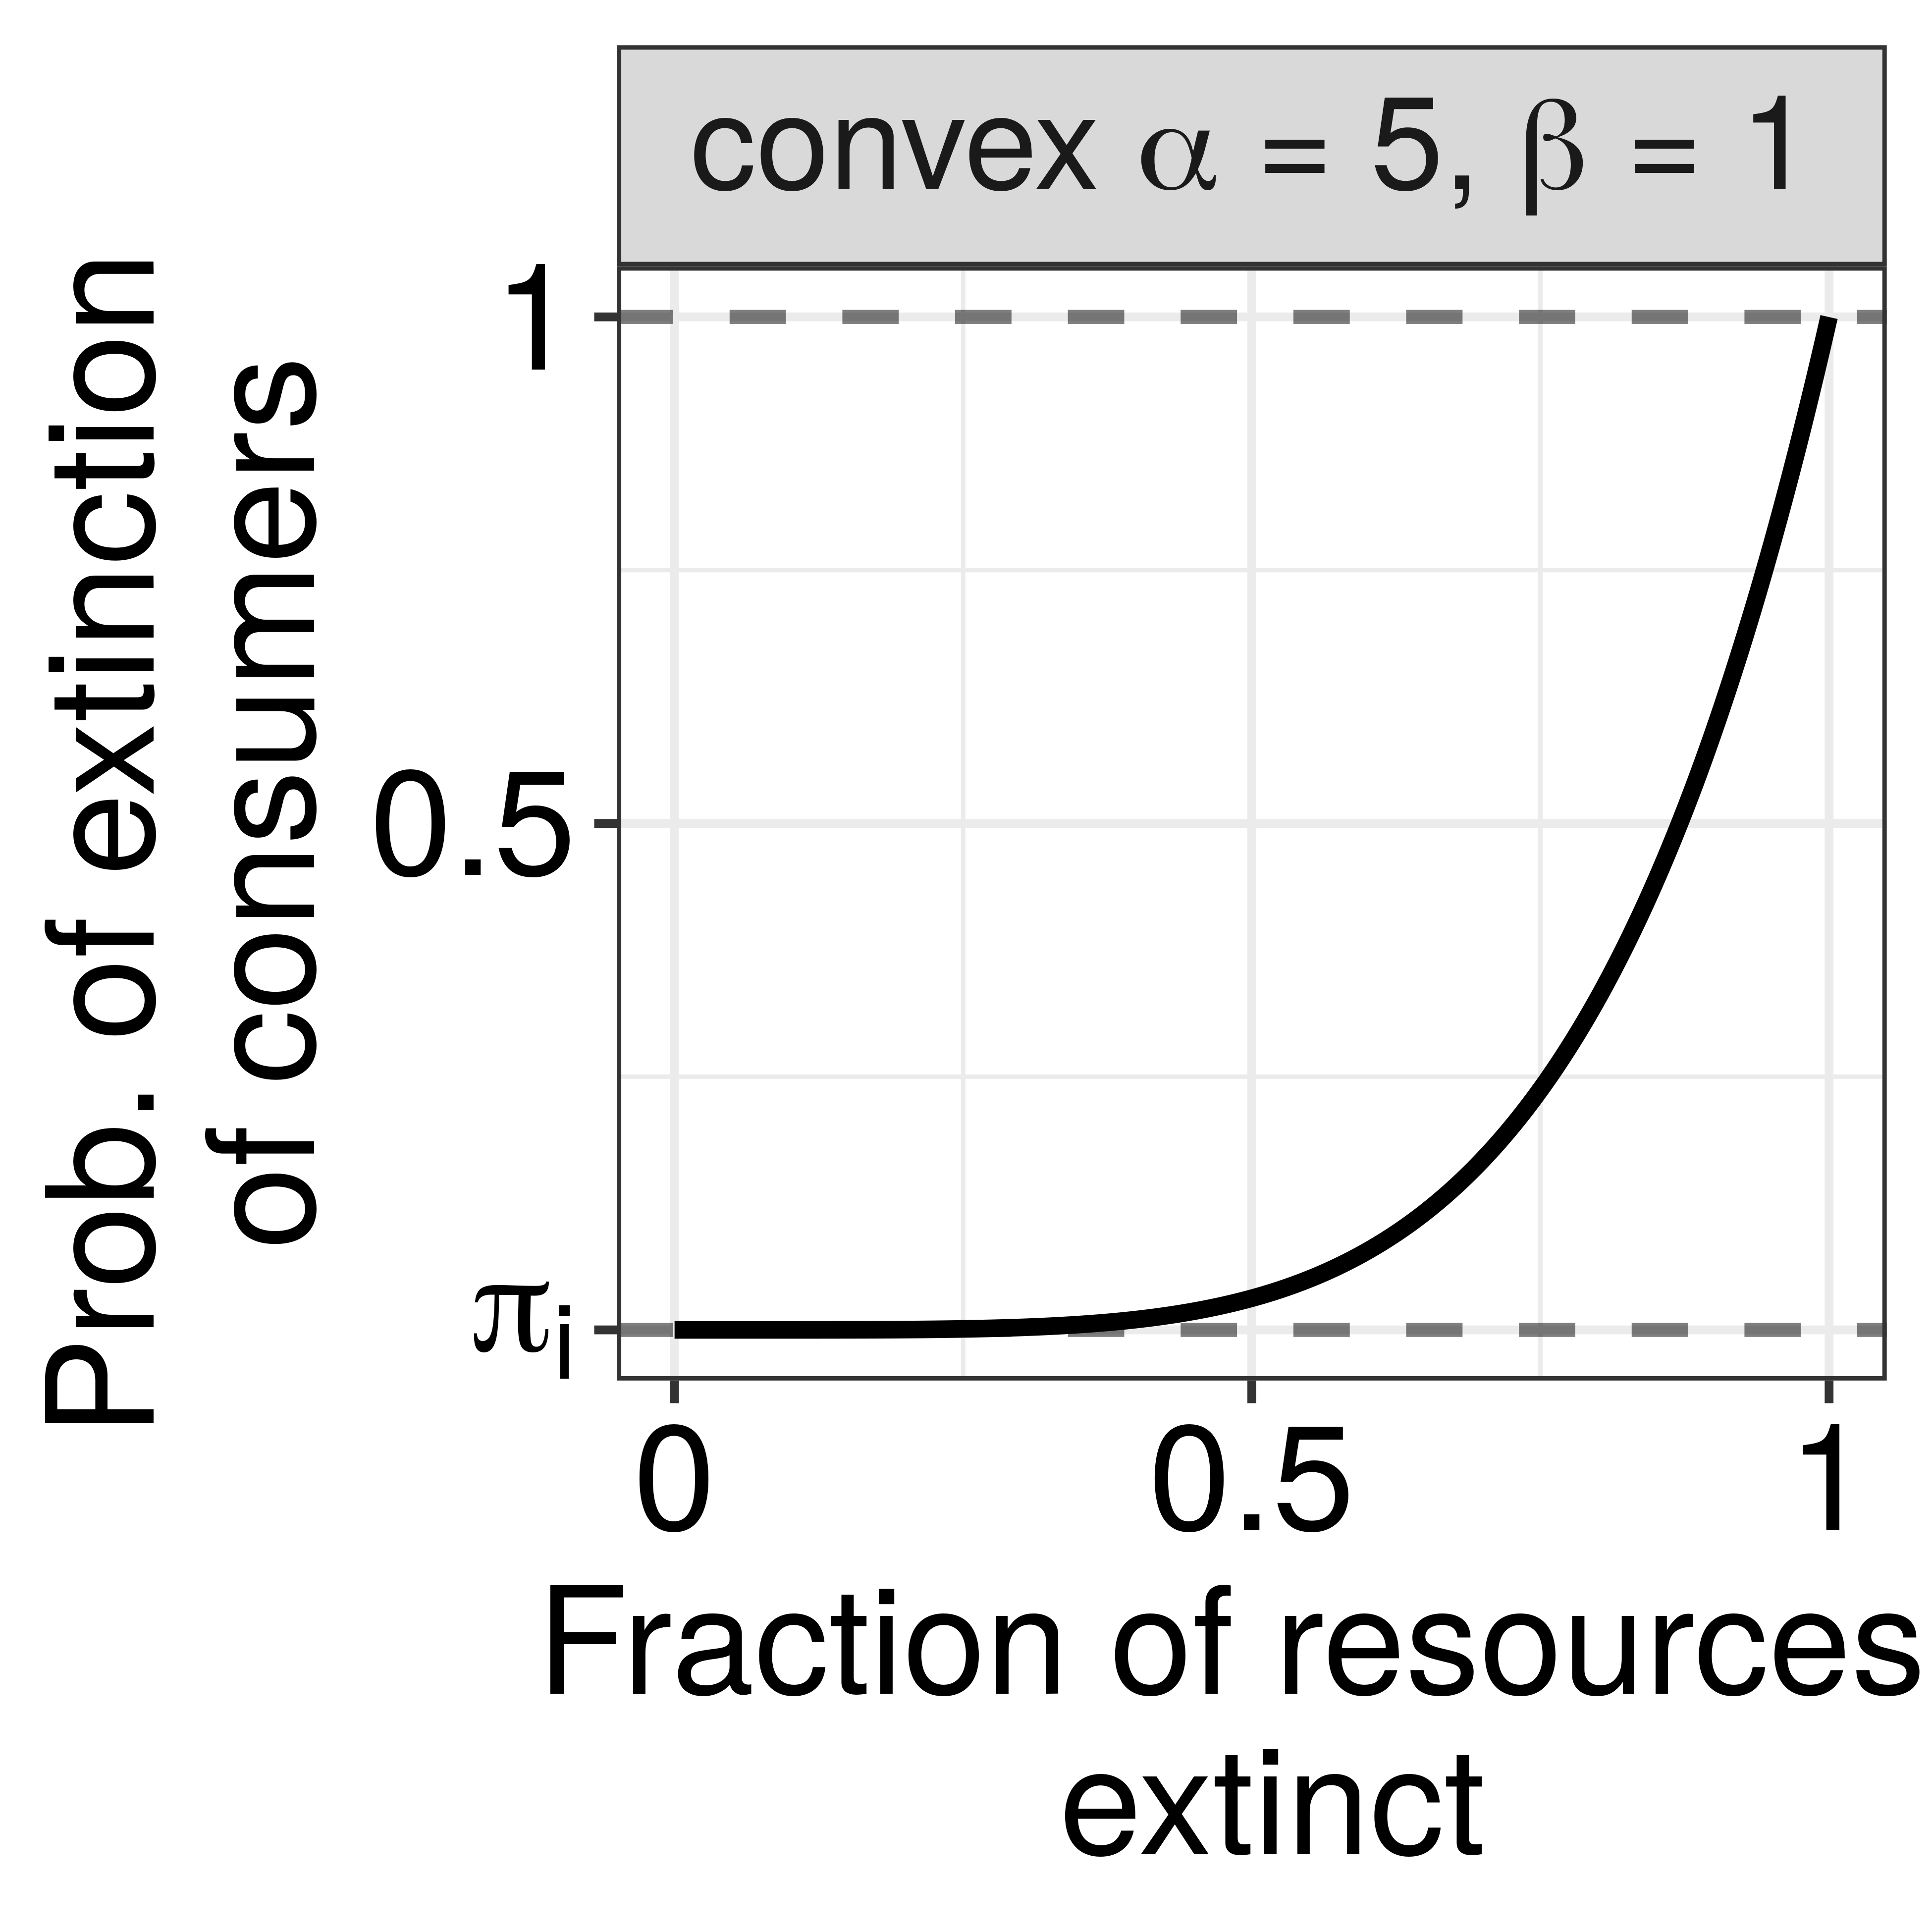
\includegraphics[width=0.19\textwidth,valign=t]{fform_5_1.png}
  \caption{Figure continued.}
  \label{fig:patchloss_web5_51}
\end{figure}

\begin{figure}\ContinuedFloat
  \includegraphics[width=0.8\textwidth,valign=t]{lambda_Model_food_web_with_350_consumer_and_50_basal_species_(5)_Weighted_basal_1_5.pdf}
  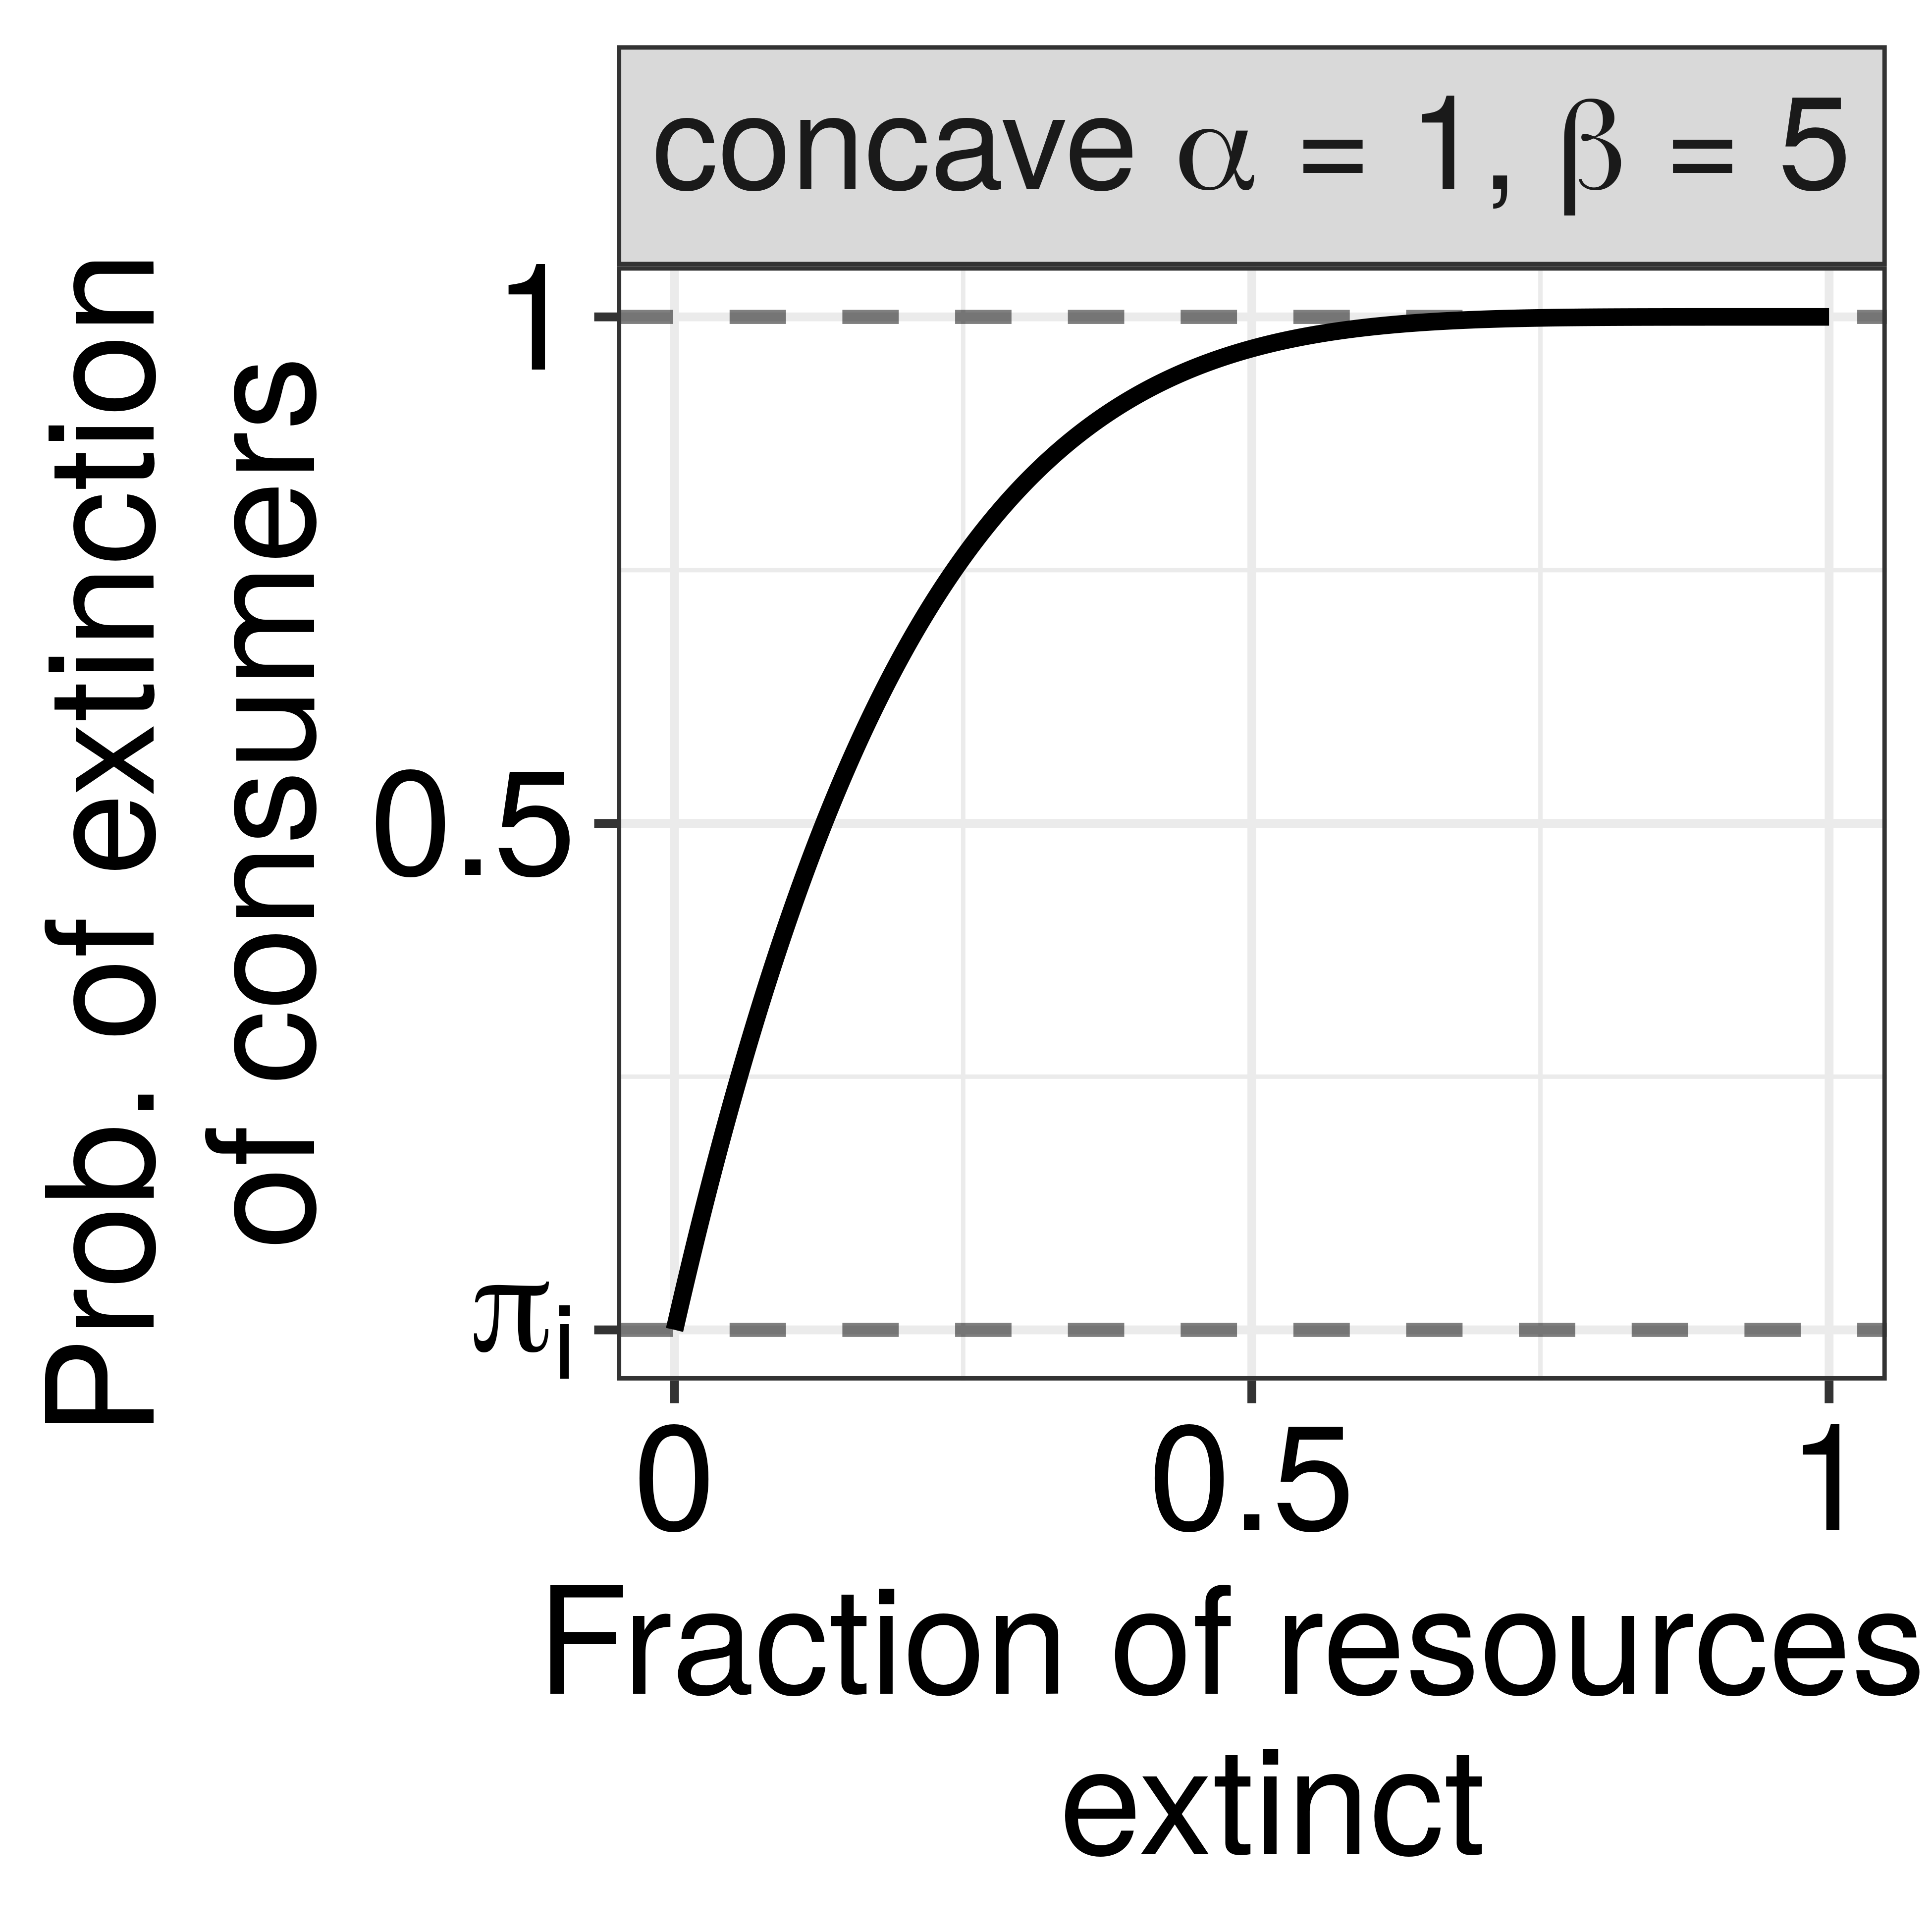
\includegraphics[width=0.19\textwidth,valign=t]{fform_1_5.png}
  \includegraphics[width=0.8\textwidth,valign=t]{lambda_Model_food_web_with_350_consumer_and_50_basal_species_(5)_Not_weighted_basal_1_5.pdf}
  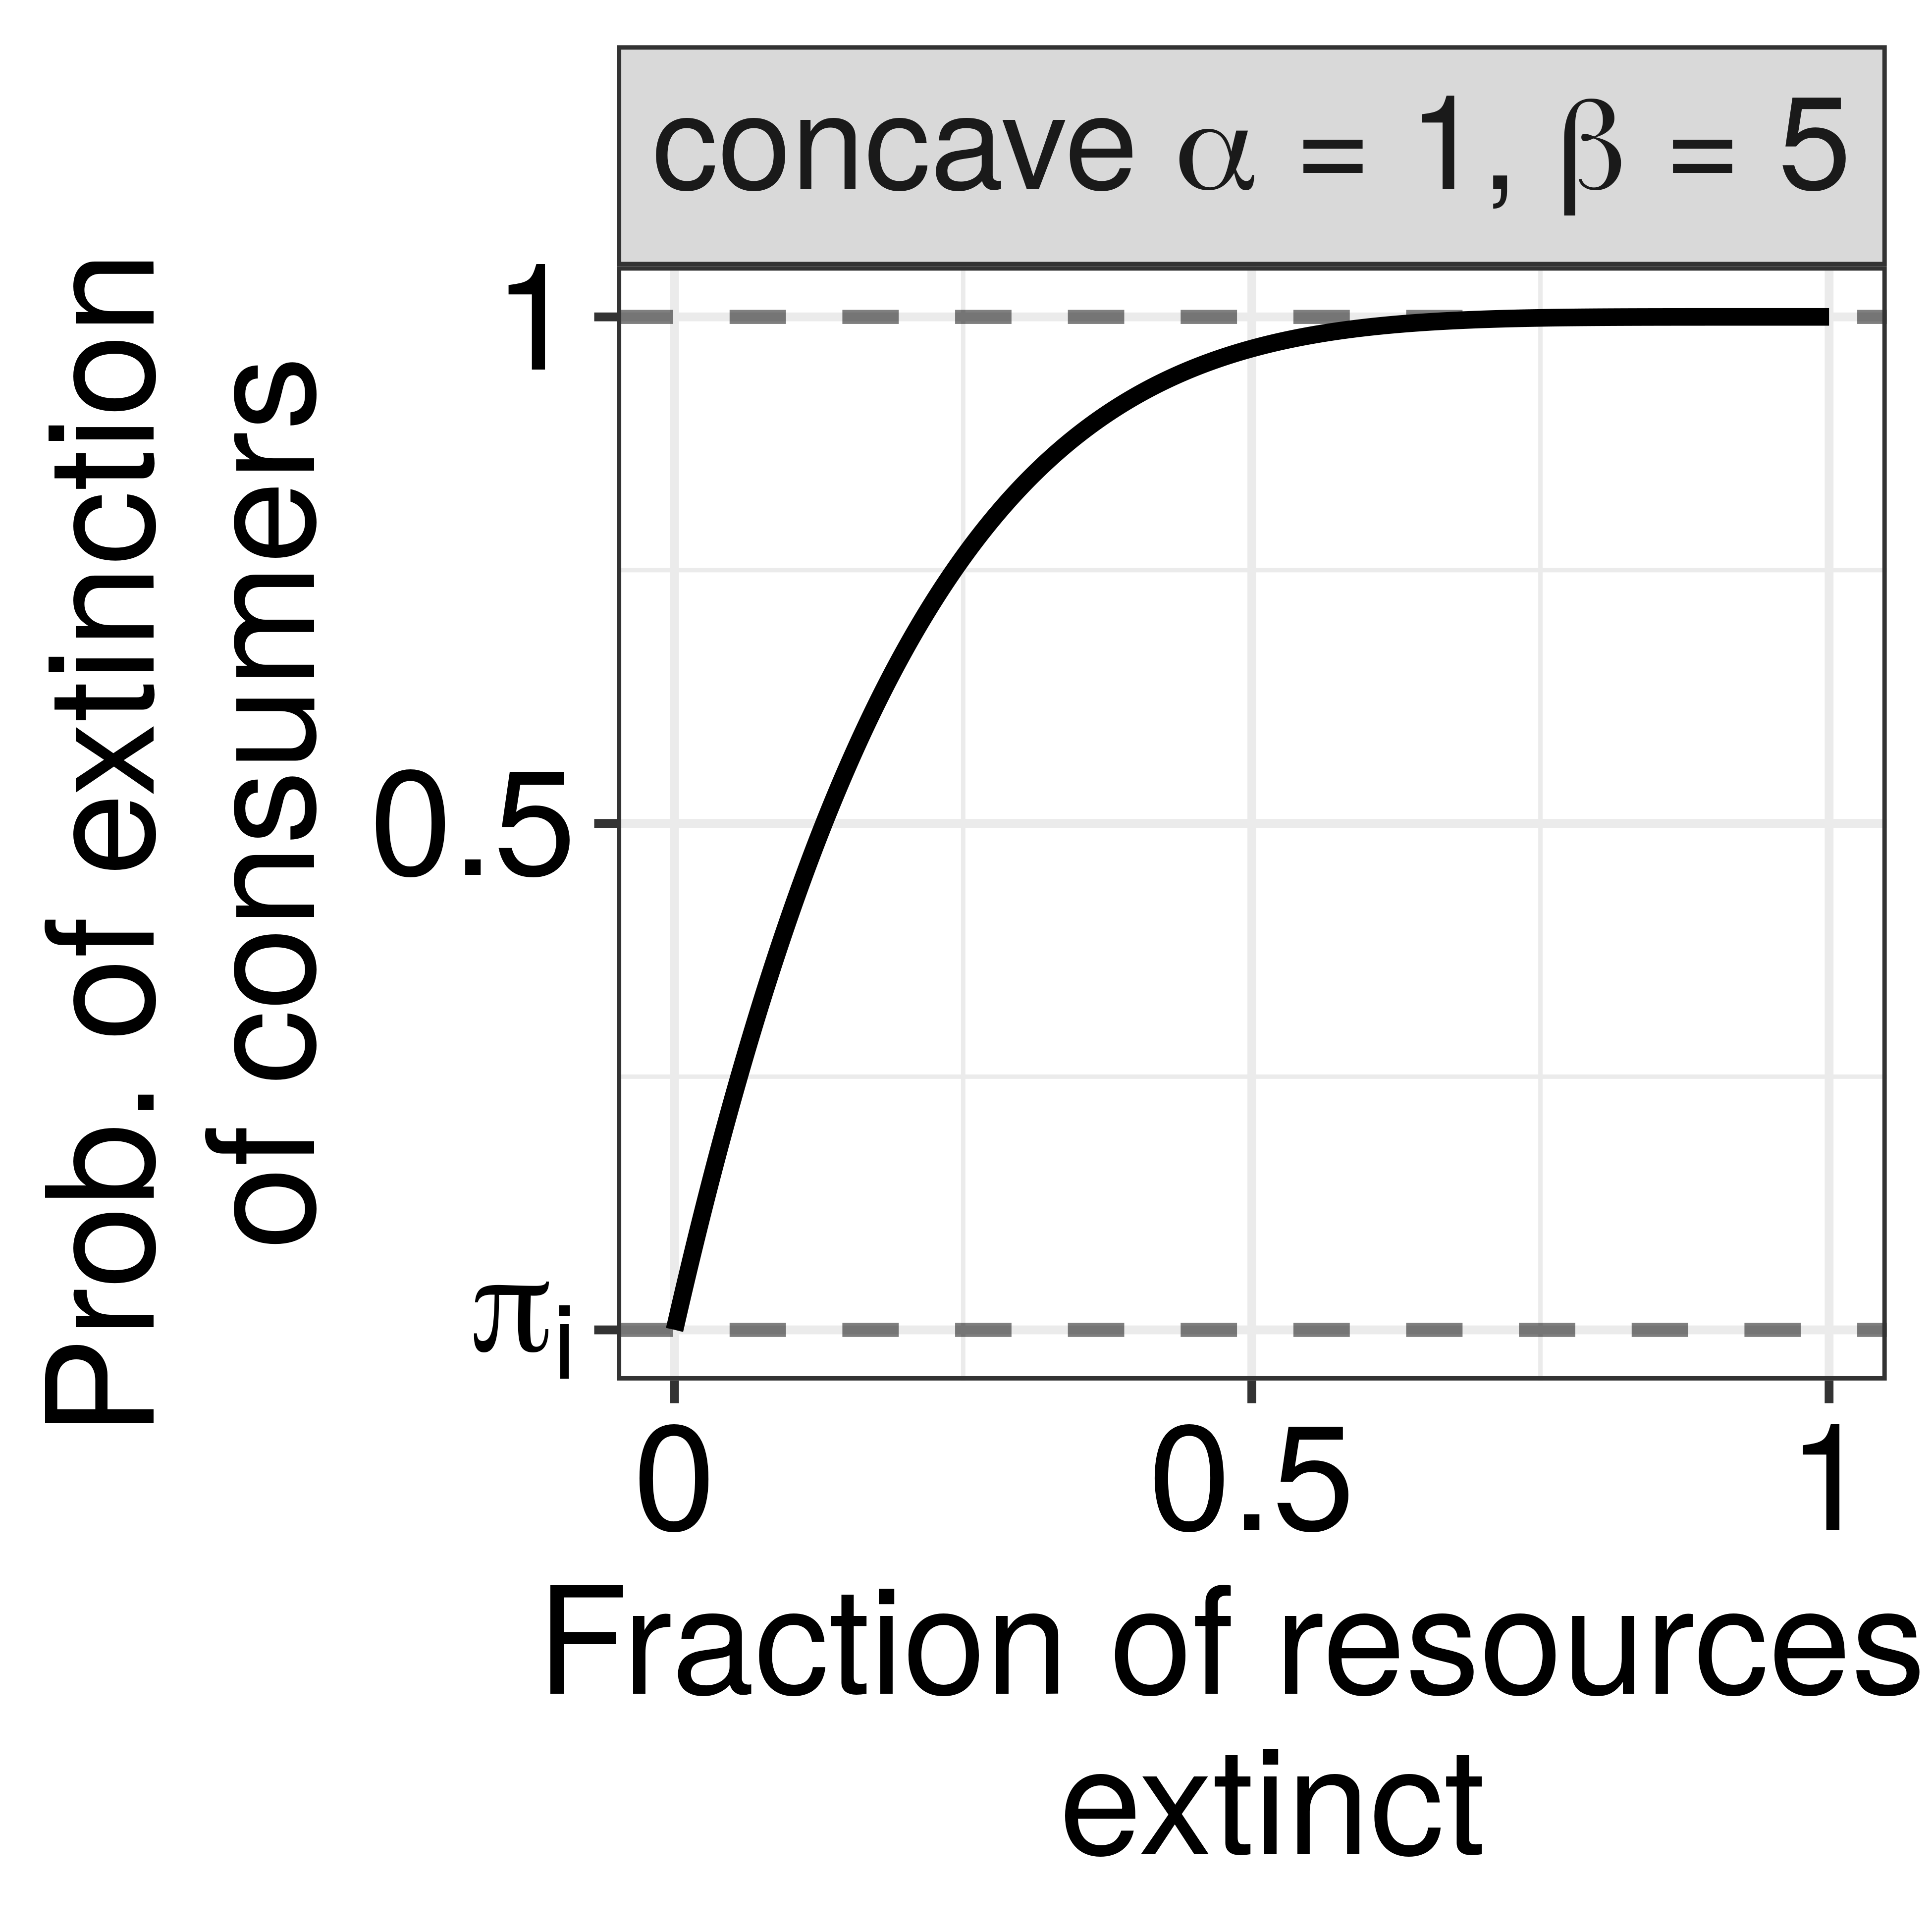
\includegraphics[width=0.19\textwidth,valign=t]{fform_1_5.png}
  \caption{Figure continued.}
  \label{fig:patchloss_web5_15}
\end{figure}

\begin{figure}\ContinuedFloat
  \includegraphics[width=0.8\textwidth,valign=t]{lambda_Model_food_web_with_350_consumer_and_50_basal_species_(5)_Weighted_basal_5_5.pdf}
  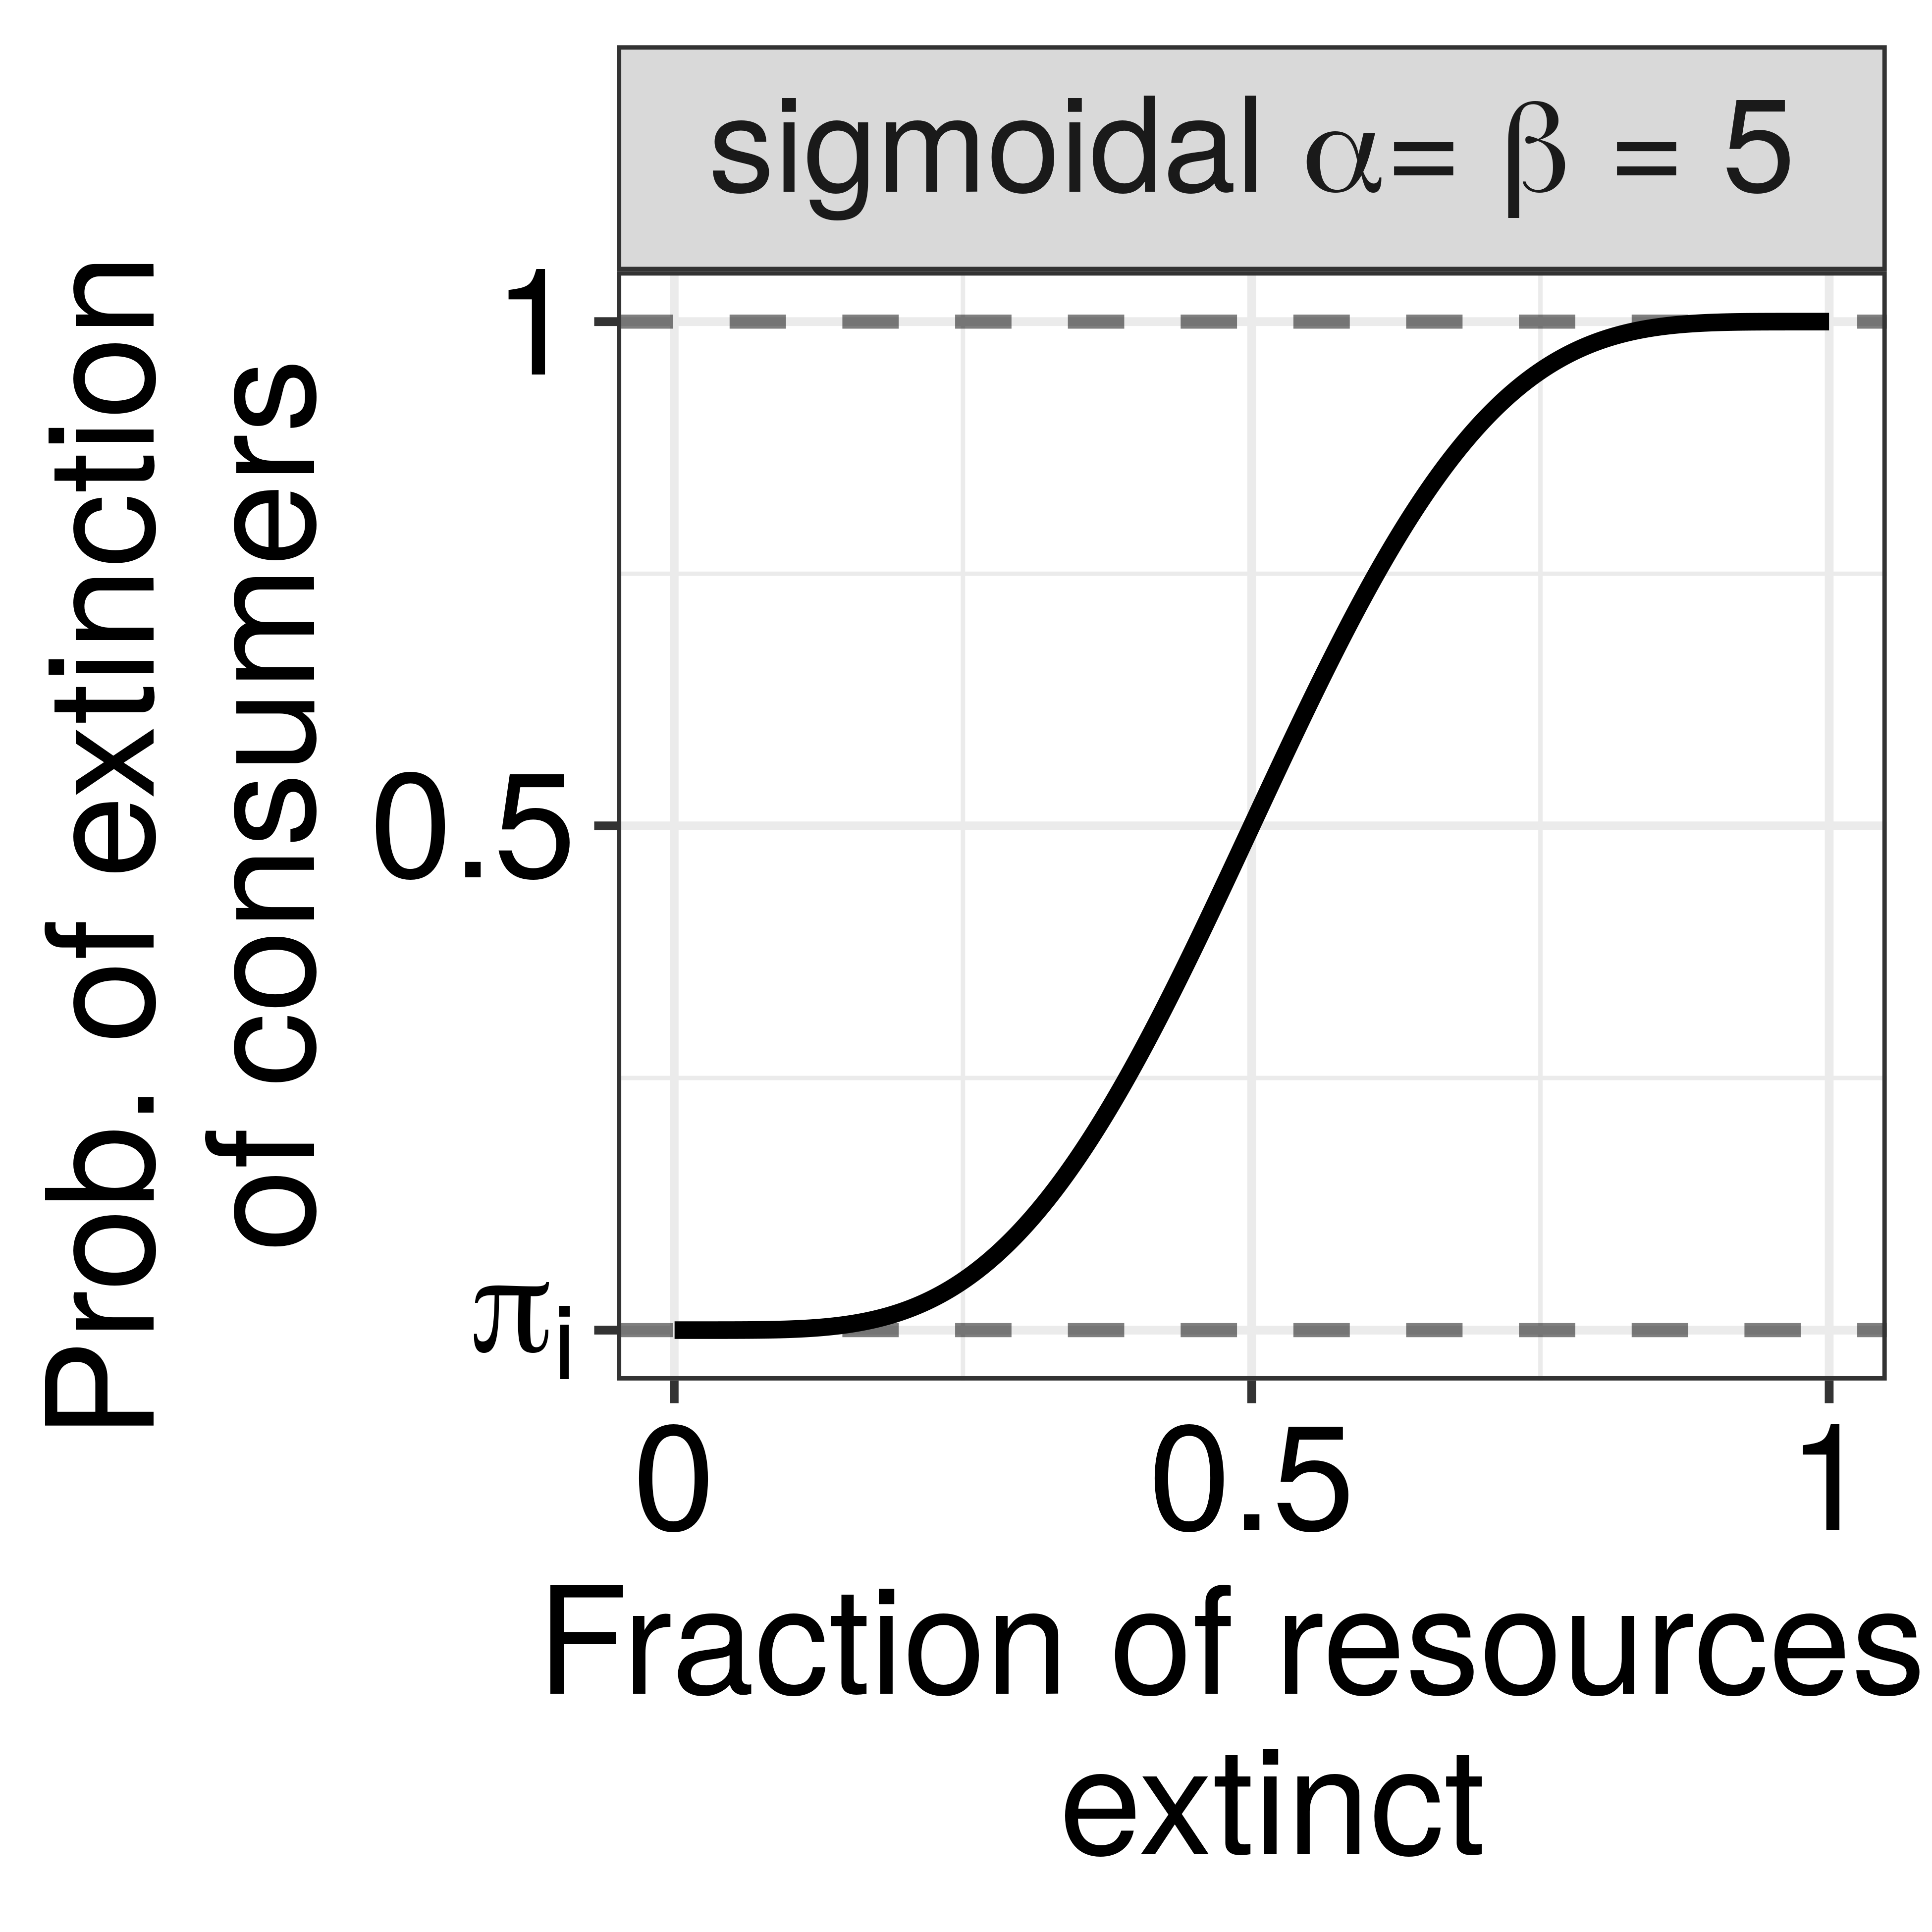
\includegraphics[width=0.19\textwidth,valign=t]{fform_5_5.png}
  \includegraphics[width=0.8\textwidth,valign=t]{lambda_Model_food_web_with_350_consumer_and_50_basal_species_(5)_Not_weighted_basal_5_5.pdf}
  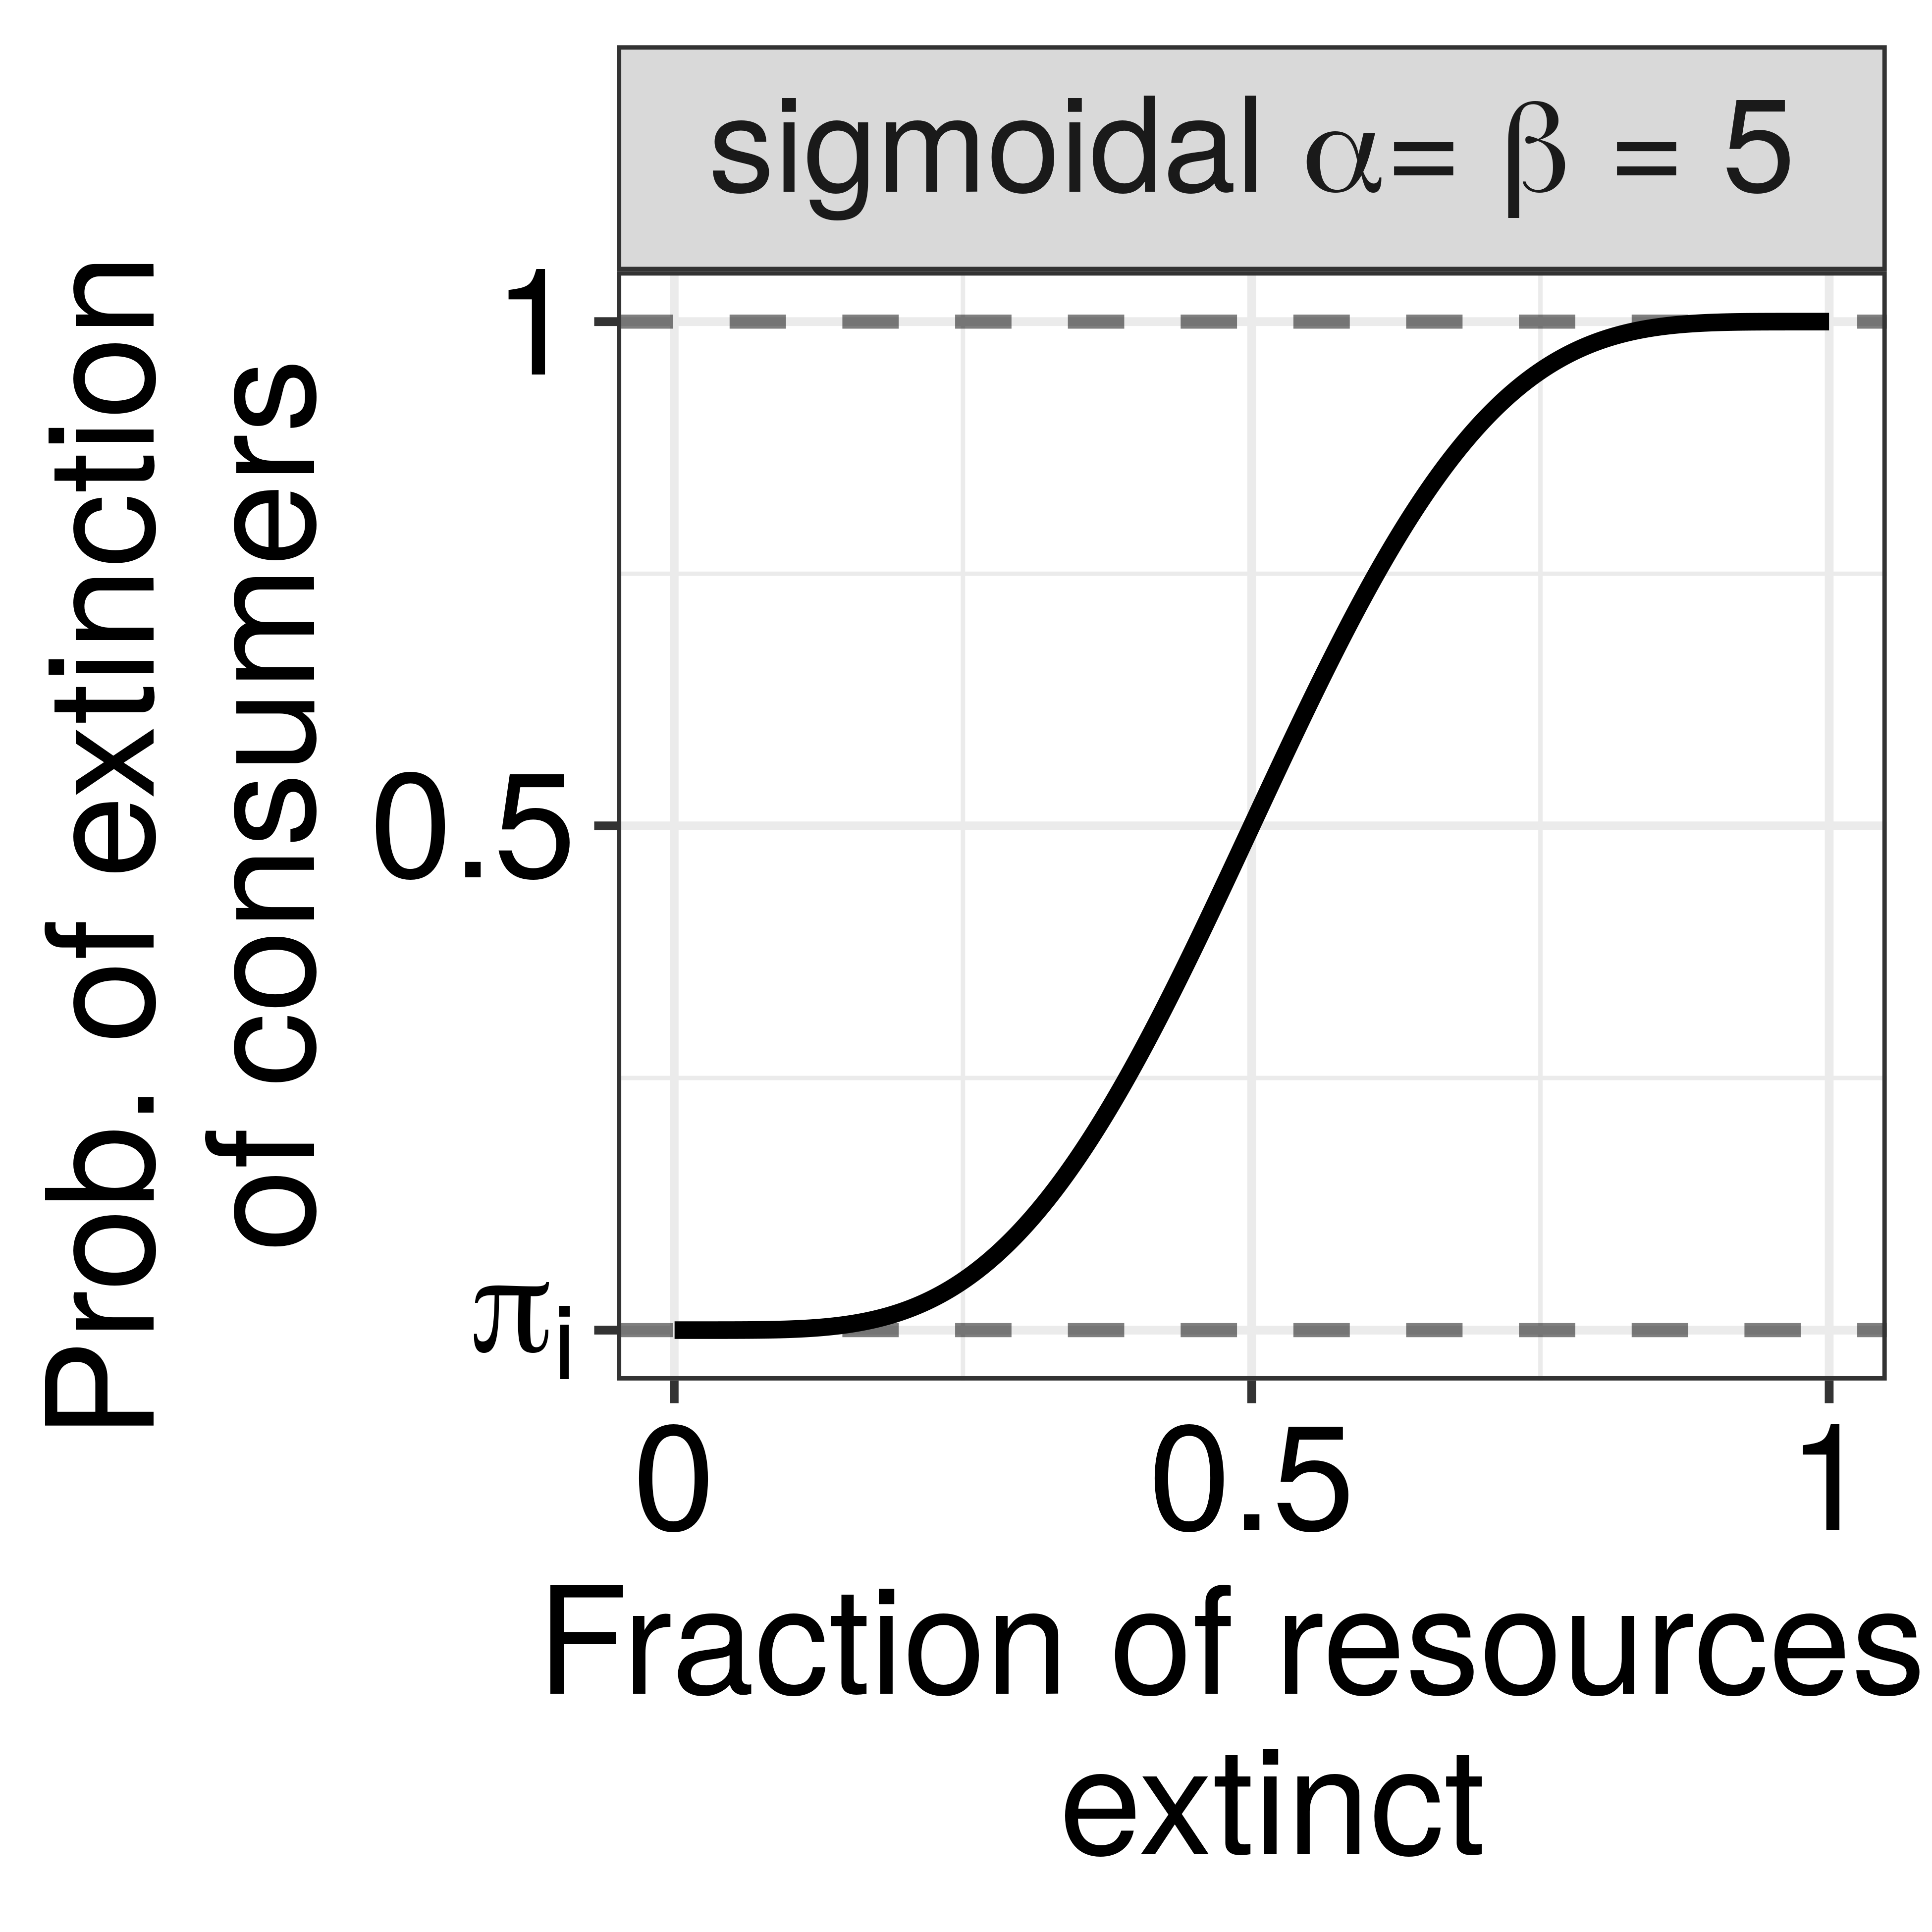
\includegraphics[width=0.19\textwidth,valign=t]{fform_5_5.png}
  \caption{Figure continued.}
  \label{fig:patchloss_web5_55}
  
\end{figure}
\end{document}

